\documentclass[12pt,a4paper,openany]{book}

\usepackage{cmap}
\usepackage[left=1.3cm, right=1.3cm, top=1.4cm, bottom=1.3cm]{geometry}
\usepackage[utf8]{inputenc}
\usepackage[english, russian]{babel}
\usepackage{indentfirst}
\usepackage{amsmath}
\usepackage{amssymb}
\usepackage{amsthm}
\usepackage{gensymb}
\usepackage{mathrsfs}
\usepackage{bm}
\usepackage{perpage}
\usepackage{enumitem}
\usepackage[unicode, colorlinks=true%,%
%linkcolor=black, pagecolor=black%
]{hyperref}
\hypersetup{pdftitle={Лекции по ВИ и УМФ.}, pdfauthor={Г. М. Жислин}}
\usepackage{tikz}
\usepackage{tabularx}
\usepackage{graphicx}
\usepackage{xfrac}
\usepackage{tocloft}    
\usepackage{titlesec} \titlelabel{\thetitle.\quad}

\setcounter{tocdepth}{1}

%\setlength{\mathindent}{0em}

\addto{\captionsrussian}{\renewcommand{\contentsname}{Содержание}}
\addto{\captionsrussian}{\renewcommand{\chaptername}{Лекция}}

\newcommand {\defeq}{\stackrel{\hspace{0.09 cm}de\!f}{=}}
\newcommand {\eqdef}{\defeq}
\newcommand{\iffdef}{\stackrel{\hspace{0.09 cm}de\!f}{\iff}}
\newcommand{\R}{\ensuremath{\mathbb{R}}}
\newcommand{\Cf}{\ensuremath{\mathcal{C}}}
\newcommand{\J}{\ensuremath{\mathcal{J}}}
\newcommand{\mc}[1]{\ensuremath{\mathcal{#1}}}
\newcommand{\ms}[1]{\ensuremath{\mathscr{#1}}}
\newcommand{\Cfn}[2][]{\ensuremath{\Cf{\mathstrut}^{#2}_{#1}}}
\newcommand{\der}[2]{\ensuremath{\frac{d#1}{d#2}}}
\newcommand{\dder}[2]{\ensuremath{\frac{d^2#1}{d#2^2}}}
\newcommand{\pder}[2]{\ensuremath{\frac{\partial#1}{\partial#2}}}
\newcommand{\pdder}[2]{\ensuremath{\frac{\partial^2#1}{\partial#2^2}}}
\newcommand{\eps}{\varepsilon}
\newcommand{\K}{\mc{K}}
\newcommand{\LL}{\ensuremath{L}}
\newcommand{\fL}[1][{[a,b]}]{\ensuremath{\mathscr{L}\hspace*{-0.11 cm}{\mathstrut}_{2}{\scriptstyle#1}}}
\newcommand{\norm}[1]{\ensuremath{\left\|#1\right\|}}
\newcommand{\Ul}[1][\lambda]{\ensuremath{\mc{U}\!{\mathstrut}_{#1}}}
\newcommand{\fLr}[1][{[a,b];\rho}]{\ensuremath{\mathscr{L}\hspace*{-0.11 cm}{\mathstrut}_{2}{\scriptstyle\left(\vphantom{A^b}#1\right)}}}
\newcommand{\dd}{\ensuremath{d}}
\newcommand{\fLone}[1][]{\ensuremath{\mathscr{L}\hspace*{-0.11 cm}{\mathstrut}_{1}{\scriptstyle#1}}}
\newcommand{\psihat}{\ensuremath{\widehat{\vphantom{\phi}\smash{\!\psi}}}}

\DeclareMathOperator{\Tang}{tg}
\DeclareMathOperator{\Div}{div}
\DeclareMathOperator{\grad}{grad}



\pagestyle{headings}

\theoremstyle{definition}
\newtheorem{_def}{Определение}[section]
\newtheorem*{_definition}{Определение}
\newtheorem{_lemm}{Лемма}[section]
\newtheorem{_teor}{Теорема}[section]
\newtheorem*{_rem}{Замечание}
\newtheorem*{_con}{Следствие}
\MakePerPage{footnote}

\setlist[enumerate,1]{label=\alph*), ref=\alph*)}

\newlist{enumerate1}{enumerate}{1}
\setlist[enumerate1,1]{label=\arabic*), ref=\arabic*)}
\newlist{enumerateA}{enumerate}{1}
\setlist[enumerateA,1]{label=\Alph*), ref=\Alph*)}

\newlist{enumerateD}{enumerate}{2}
\setlist[enumerateD,1]{label=\arabic*., ref=\arabic*.}
\setlist[enumerateD,2]{{label=\alph*., ref=\alph*.}}

\newlist{enumerateBr}{enumerate}{1}
\setlist[enumerateBr,1]{label=\underline{(\arabic*)}, ref=\underline{(\arabic*)}}

\newlist{enumerateP1}{enumerate}{1}
\setlist[enumerateP1,1]{label=п.\,\arabic*.,ref=п.\,\arabic*.}

\newlist{enumeraterm}{enumerate}{1}
\setlist[enumeraterm,1]{label=\roman*),ref=\roman*)}

\newlist{enumerateAi}{enumerate}{1}
\setlist[enumerateAi,1]{label=(\Alph*$_{i}$), ref=(\Alph*$_i$)}

\nofiles

\def\?#1{#1\nobreak\discretionary{}{\hbox{$\mathsurround=0pt #1$}}{}}

\begin{document}
	

	
	
	\author{Г.\,М.~Жислин}
	\title{Лекции по вариационному исчислению и уравнениям математической физики}
	\date{Конспектировал А.\,Г.~Чубаров}
	
	
	
	\maketitle
	\tableofcontents
	
	\renewcommand{\thepart}{\Asbuk{part}}
	\renewcommand{\thechapter}{\arabic{chapter}}
	\renewcommand{\thesection}{\arabic{section}}
	\renewcommand{\thesubsection}{\Roman{subsection}}
	\renewcommand{\thefootnote}{\roman{footnote}}
	\renewcommand{\phi}{\varphi}
	\renewcommand{\Re}{\ensuremath{\mc{R}e\,}}
	\renewcommand{\Im}{\ensuremath{\mc{I}m\,}}
	\numberwithin{equation}{section}
	
	\part{Вариационное исчисление.}
	\label{part1}
	\chapter{}
\label{lecture1}
Мы начинаем первую часть нашего курса. Эта часть --- <<Вариационное исчисление>>.
\section{Определение функционала. Примеры вариационных задач.}
\label{lecture1section1}
До сих пор вам в основном встречалось два типа зависимостей:
\begin{enumerate}
	\item Функция: каждому числу или совокупности чисел (в случае функции многих переменных) ставится в соответствие число или совокупность чисел (в случае вектор-функции).
	
	\item Оператор: каждой функции или набору функций ставится в соответствии функция или набор функций. Например, если рассматривать оператор дифференцирования на функциях имеющих производную, то $f(x)\to f'(x)$, или $f(x_1,\ldots,x_n)\?\to f(\phi_1(x_1),\ldots,\phi_n(x_n))$, где $\phi_i(x_i)$ --- некоторые функции.
	
\end{enumerate}

Вариационное исчисление изучает другие зависимости --- когда каждой функции или набору функций из определённого класса ставится в соответствие число.\\
Примеры:
\begin{enumerate1}
	\item $S[f]=\int\limits_a^b f(x)\,\dd{x}$ --- площадь заштрихованной фигуры, $f(x)\in \Cfn[{[a,b]}]{}$.
	\begin{figure}[H]\centering
	\tikzset{every picture/.style={line width=0.75pt}} %set default line width to 0.75pt        
	
	\begin{tikzpicture}[x=0.75pt,y=0.75pt,yscale=-1,xscale=1]
		%uncomment if require: \path (0,142); %set diagram left start at 0, and has height of 142
		
		%Shape: Axis 2D [id:dp819600743870198] 
		\draw  (57,105) -- (208,105)(72.1,15) -- (72.1,115) (201,100) -- (208,105) -- (201,110) (67.1,22) -- (72.1,15) -- (77.1,22)  ;
		%Curve Lines [id:da06782546481569751] 
		\draw    (91,51) .. controls (131,21) and (151,81) .. (191,51) ;
		%Straight Lines [id:da30279113153735726] 
		\draw  [dash pattern={on 4.5pt off 4.5pt}]  (91,51) -- (91,105.5) ;
		%Straight Lines [id:da6946884097796024] 
		\draw  [dash pattern={on 4.5pt off 4.5pt}]  (191,51) -- (191,105.5) ;
		%Straight Lines [id:da08980597198305262] 
		\draw [color={rgb, 255:red, 155; green, 155; blue, 155 }  ,draw opacity=1 ]   (191,77.25) -- (163,105.25) ;
		%Straight Lines [id:da18207740263127015] 
		\draw [color={rgb, 255:red, 155; green, 155; blue, 155 }  ,draw opacity=1 ]   (191,51) -- (136.5,105.5) ;
		%Straight Lines [id:da7156119647134078] 
		\draw [color={rgb, 255:red, 155; green, 155; blue, 155 }  ,draw opacity=1 ]   (157,59) -- (110.5,105.5) ;
		%Straight Lines [id:da5864249578728782] 
		\draw [color={rgb, 255:red, 155; green, 155; blue, 155 }  ,draw opacity=1 ]   (138,50.5) -- (91.5,97) ;
		%Straight Lines [id:da25902283366089773] 
		\draw [color={rgb, 255:red, 155; green, 155; blue, 155 }  ,draw opacity=1 ]   (119,42.5) -- (91,70.5) ;
		
		% Text Node
		\draw (91,111.9) node [anchor=north west][inner sep=0.75pt]    {$a$};
		% Text Node
		\draw (191,108.9) node [anchor=north west][inner sep=0.75pt]    {$b$};
		
		
	\end{tikzpicture}
	\caption{~}
	\label{l1:fig:1}
	\end{figure}
	\item $l[f]=\int\limits_a^b\sqrt{1+f^{\prime 2}(x)}\,\dd{x}$ --- длина кривой, $f\in \Cfn[{[a,b]}]{1}$ --- класс непрерывно дифференцируемых на ${[a,b]}$ функций.
\end{enumerate1}

\noindent Дадим общее определение для подобного рода зависимостей.
\begin{Def}
	Пусть $\mc{K}=\{f(x_1,\ldots,x_n)\}$ --- класс каких-то функций $f(x_1,\ldots,x_n)$, определённых в области $\mc{D}$ $n$-мерного пространства. Будем говорить, что \textbf{задан функционал $\pmb{\J[f]}$}, если задан закон, по которому каждой функции $f\in\mc{K}$ ставится в соответствие число $\J[f]$. Это число обозначается $\J[f]$ и называется значением функционала на функции $f$.
\end{Def}

\noindent В приведённых выше примерах \\
\indent$S[f]$ задан на $\mc{K}=\big\{f(x)\big|f\in \Cfn[{[a,b]}]{}\big\}$,\\
\indent $l[f]$ задан на $\mc{K}=\big\{f(x)\big|f\in \Cfn[{[a,b]}]{1}\big\}$.\\
Разумеется, могут быть и другие классы для функционалов $S[f]$ и $l[f]$ в зависимости от рассматриваемых задач.

Исследуя свойства функций в курсе математики, вы решали задачи о нахождении экстремумов функций, однако целый ряд задач требует отыскания экстремумов не функций, а функционалов. Именно этим и занимается <<Вариационное исчисление>>.
\vspace{0.25cm}

Приведём примеры задач, решаемых в вариационном исчислении.
\newlist{enumerate2}{enumerate}{1}
\setlist[enumerate2,1]{label=\arabic*., ref=\arabic*.} 

\begin{enumerate2}
	\item \textbf{Задача о кривой наискорейшего спуска (задача о брахистохроне)}.\\
	Пусть на вертикальной плоскости $x,y$ заданы две точки $A(a, y_0)$ и $B(b, y_1)$, $y_1<y_0$.
	
	\begin{figure}[H]\centering
	\tikzset{every picture/.style={line width=0.75pt}} %set default line width to 0.75pt        
	
	\begin{tikzpicture}[x=0.75pt,y=0.75pt,yscale=-1,xscale=1]
		%uncomment if require: \path (0,142); %set diagram left start at 0, and has height of 142
		
		%Shape: Axis 2D [id:dp5296256236644323] 
		\draw  (57,105) -- (208,105)(72.1,15) -- (72.1,115) (201,100) -- (208,105) -- (201,110) (67.1,22) -- (72.1,15) -- (77.1,22)  ;
		%Curve Lines [id:da5139961929878707] 
		\draw    (91,23.5) .. controls (116,64.5) and (150,65.5) .. (191,61.5) ;
		%Straight Lines [id:da7749819981896289] 
		\draw  [dash pattern={on 4.5pt off 4.5pt}]  (91,23.5) -- (91,105.5) ;
		%Straight Lines [id:da17627525123267485] 
		\draw  [dash pattern={on 4.5pt off 4.5pt}]  (191,61.5) -- (191,105.5) ;
		
		% Text Node
		\draw (93,108.9) node [anchor=north west][inner sep=0.75pt]    {$a$};
		% Text Node
		\draw (193,108.9) node [anchor=north west][inner sep=0.75pt]    {$b$};
		% Text Node
		\draw (92,8.4) node [anchor=north west][inner sep=0.75pt]    {$A( a,y_{0})$};
		% Text Node
		\draw (191,45.4) node [anchor=north west][inner sep=0.75pt]    {$B( b,y_{1})$};
		% Text Node
		\draw (119,66.4) node [anchor=north west][inner sep=0.75pt]    {$y( x)$};
		
		
	\end{tikzpicture}
	\caption{~}
	\label{l1:fig:2}
	\end{figure}
	Задача: найти кривую, соединяющую точки $A$ и $B$, по которой материальная точка скатится из $A$ в $B$ за минимальное время.
	
	Пусть $y(x)$ --- произвольная допустимая кривая. Найдём время скатывания по этой кривой. Разобъём отрезок ${[a,b]}$ на $n$ частей 
	\begin{equation*}
		\Delta x\eqdef\dfrac{b-a}{n}
	\end{equation*} 
	и определим время скатывания по элементарному отрезку кривой над $\Delta x$.
	\begin{figure}[H]\centering
	\tikzset{every picture/.style={line width=0.75pt}} %set default line width to 0.75pt        
	
	\begin{tikzpicture}[x=0.75pt,y=0.75pt,yscale=-1,xscale=1]
		%uncomment if require: \path (0,142); %set diagram left start at 0, and has height of 142
		
		%Shape: Axis 2D [id:dp3120006234200525] 
		\draw  (57,105) -- (208,105)(72.1,15) -- (72.1,115) (201,100) -- (208,105) -- (201,110) (67.1,22) -- (72.1,15) -- (77.1,22)  ;
		%Curve Lines [id:da5633806752426602] 
		\draw    (91,23.5) .. controls (116,64.5) and (150,65.5) .. (191,61.5) ;
		%Straight Lines [id:da19712351894158475] 
		\draw  [dash pattern={on 4.5pt off 4.5pt}]  (91,23.5) -- (91,105.5) ;
		%Straight Lines [id:da4773530776083561] 
		\draw  [dash pattern={on 4.5pt off 4.5pt}]  (191,61.5) -- (191,105.5) ;
		%Straight Lines [id:da5754475621627722] 
		\draw    (71.1,105) -- (205,105) (91.1,101) -- (91.1,109)(111.1,101) -- (111.1,109)(131.1,101) -- (131.1,109)(151.1,101) -- (151.1,109)(171.1,101) -- (171.1,109)(191.1,101) -- (191.1,109) ;
		%Straight Lines [id:da416850289861296] 
		\draw    (113,59) -- (132.05,59) ;
		%Straight Lines [id:da9627818333382503] 
		\draw    (113,48.5) -- (113,59) ;
		%Flowchart: Connector [id:dp8284141548912727] 
		\draw  [fill={rgb, 255:red, 0; green, 0; blue, 0 }  ,fill opacity=1 ] (119,105) .. controls (119,103.9) and (119.9,103) .. (121,103) .. controls (122.1,103) and (123,103.9) .. (123,105) .. controls (123,106.1) and (122.1,107) .. (121,107) .. controls (119.9,107) and (119,106.1) .. (119,105) -- cycle ;
		%Flowchart: Connector [id:dp5793213628332867] 
		\draw  [fill={rgb, 255:red, 0; green, 0; blue, 0 }  ,fill opacity=1 ] (119,54) .. controls (119,52.9) and (119.9,52) .. (121,52) .. controls (122.1,52) and (123,52.9) .. (123,54) .. controls (123,55.1) and (122.1,56) .. (121,56) .. controls (119.9,56) and (119,55.1) .. (119,54) -- cycle ;
		
		% Text Node
		\draw (93,108.9) node [anchor=north west][inner sep=0.75pt]    {$a$};
		% Text Node
		\draw (193,108.9) node [anchor=north west][inner sep=0.75pt]    {$b$};
		% Text Node
		\draw (93,3.4) node [anchor=north west][inner sep=0.75pt]    {$A( a,y_{0})$};
		% Text Node
		\draw (191,41.4) node [anchor=north west][inner sep=0.75pt]    {$B( b,y_{1})$};
		% Text Node
		\draw (152,65.4) node [anchor=north west][inner sep=0.75pt]    {$y( x)$};
		% Text Node
		\draw (115,62.4) node [anchor=north west][inner sep=0.75pt]  [font=\scriptsize]  {$\Delta x$};
		% Text Node
		\draw (96,47.4) node [anchor=north west][inner sep=0.75pt]  [font=\scriptsize]  {$\Delta y$};
		% Text Node
		\draw (121,108.4) node [anchor=north west][inner sep=0.75pt]  [font=\scriptsize]  {$x_{i}$};
		% Text Node
		\draw (122,38.4) node [anchor=north west][inner sep=0.75pt]  [font=\scriptsize]  {$y( x_{i})$};
		
		
	\end{tikzpicture}
	\caption{~}
	\label{l1:fig:3}
	\end{figure}
	Длина этого участка
	\begin{equation*}
		\sqrt{(\Delta x)^2+(\Delta y)^2}=\sqrt{1+\left(\frac{\Delta y}{\Delta x}\right)^2}\cdot \Delta x.
	\end{equation*}
	Пусть $v(x_i, y_i)$ --- скорость на участке $\Delta x$. Тогда элементарное время скатывания
	\begin{equation*}
		\Delta t= \displaystyle \frac{\sqrt{1+\left(\frac{\Delta y}{\Delta x}\right)^2}\cdot \Delta x}{v(x_i, y_i)}. 
	\end{equation*}
	Суммируя по всем элементарным участкам $\Delta x$ и переходя к пределу при $n\to\infty$, получим время скатывания по кривой $y(x)$.
	\begin{equation*}
		 T[y]=\int\limits_a^b\frac{\sqrt{1+y^{\prime 2}}}{v(x,y)}\,\dd{x}.
	\end{equation*}
	Величину скорости находим из закона сохранения энергии. Пусть $m$ --- масса материальной точки, начальная скорость скатывания равна 0; тогда при $x=a$ потенциальная энергия равна $m\cdot g\cdot y_0$, кинетическая равна нулю. В точке $x$ потенциальная энергия равна $m\cdot g\cdot y$, а кинетическая --- $\frac{m\cdot v^2}{2}$. Таким образом
	\begin{equation*}
		m\cdot g\cdot y_0=m\cdot g\cdot y+\frac{m\cdot v^2}{2}\quad\Rightarrow \quad v=\sqrt{2\cdot g\cdot(y_0-y)}.
	\end{equation*}
	Таким образом  
	\begin{equation*}
		 T[y]=\int\limits_a^b\frac{\sqrt{1+y^{\prime 2}}}{\sqrt{2\cdot g\cdot(y_0-y)}}\,\dd{x}.
	\end{equation*}
	
	Класс $\mc{K}$ допустимых кривых $y=y(x)$ в этой задаче описывается равенством 	
	\begin{equation*}
		\mc{K}=\big\{y(x)\big|y\in\Cfn[{[a,b]}]{1}, y(a)=y_0, y(b)=y_1\big\}.
	\end{equation*}
	Таким образом надо найти $\min\limits_{y\in\mc{K}}\,T[y]$. Функция, дающая минимум (или максимум) функционала, называется \emph{минимайзером} (или \emph{максимайзером}). Минимайзер рассматриваемой задачи --- кривая наискорейшего спуска. Она называется брахистохрона.
	
	\item \textbf{Задача о геодезических.}\\
	Пусть в пространстве $\mathbb{R}^3$ задана поверхность $\phi(x,y,z)=0$ и $A(a_0,b_0,c_0)$, $B(a_1,b_1,c_1)$ --- произвольные точки на поверхности.
	
	\begin{figure}[H]\centering
	\tikzset{every picture/.style={line width=0.75pt}} %set default line width to 0.75pt        
	
	\begin{tikzpicture}[x=0.75pt,y=0.75pt,yscale=-1,xscale=1]
		%uncomment if require: \path (0,124); %set diagram left start at 0, and has height of 124
		
		%Shape: Polygon Curved [id:ds7004080197938745] 
		\draw   (92,35) .. controls (119,1) and (189,-5) .. (204,24) .. controls (219,53) and (187,80) .. (218,96) .. controls (249,112) and (84,132) .. (92,95) .. controls (100,58) and (65,69) .. (92,35) -- cycle ;
		%Flowchart: Connector [id:dp6316722605629903] 
		\draw  [fill={rgb, 255:red, 0; green, 0; blue, 0 }  ,fill opacity=1 ] (114,93) .. controls (114,91.34) and (115.34,90) .. (117,90) .. controls (118.66,90) and (120,91.34) .. (120,93) .. controls (120,94.66) and (118.66,96) .. (117,96) .. controls (115.34,96) and (114,94.66) .. (114,93) -- cycle ;
		%Flowchart: Connector [id:dp17981276820818448] 
		\draw  [fill={rgb, 255:red, 0; green, 0; blue, 0 }  ,fill opacity=1 ] (168,22) .. controls (168,20.34) and (169.34,19) .. (171,19) .. controls (172.66,19) and (174,20.34) .. (174,22) .. controls (174,23.66) and (172.66,25) .. (171,25) .. controls (169.34,25) and (168,23.66) .. (168,22) -- cycle ;
		%Curve Lines [id:da15915648969896234] 
		\draw    (117,93) .. controls (157,63) and (131,52) .. (171,22) ;
		%Curve Lines [id:da7096853264238667] 
		\draw  [dash pattern={on 0.84pt off 2.51pt}]  (117,93) .. controls (176,67) and (113,41) .. (171,22) ;
		%Curve Lines [id:da6619831022453118] 
		\draw  [dash pattern={on 0.84pt off 2.51pt}]  (117,93) .. controls (131,63) and (178,56) .. (171,22) ;
		
		% Text Node
		\draw (122,96.4) node [anchor=north west][inner sep=0.75pt]    {$A$};
		% Text Node
		\draw (176,25.4) node [anchor=north west][inner sep=0.75pt]    {$B$};
		
		
	\end{tikzpicture}
	\caption{~}
	\label{l1:fig:4}
	\end{figure}

	Задача: проложить по поверхности кратчайший путь, соединяющий точки $A$ и $B$, то есть найти кривую минимальной длины, лежащую на поверхности и проходящую через $A$ и $B$. Кривые мы будем задавать параметрически: 
	\begin{equation*}
		\Gamma=\big\{x(t), y(t), z(t); t_0\leqslant t\leqslant t_1\big\}.
	\end{equation*}
	Класс допустимых к рассмотрению кривых определяется, во-первых, условием принадлежности к поверхности
	\begin{equation*}
		\phi(x(t),y(t),z(t))\equiv0\quad t_0\leqslant t\leqslant t_1;
	\end{equation*}
	во-вторых, условием прохождения через точки $A,\ B$: 
	\begin{equation*}
		x(t_i)=a_i, y(t_i)=b_i, z(t_i)=c_i,\quad i=0,1;
	\end{equation*}
	в-третьих: $\Gamma\in\Cfn[{[t_0,t_1]}]{1}$. 
	
	Длина кривой 
	\begin{equation*}
		 l[\Gamma]=\int\limits_{t_0}^{t_1}\sqrt{x^{\prime 2}+y^{\prime 2}+z^{\prime 2}}\,dt.
	\end{equation*}

	Мы должны минимизировать функционал $l[\Gamma]$ в классе допустимых функций, описанных выше. Кривые, дающие решение задачи на $\min\,l[\Gamma]$, называются геодезическими, и сама задача --- задача о геодезических.
	
	\item \textbf{Изопериметрическая задача}.\\
	Словесная формулировка: имеется проволока заданной длины; надо на плоскости огородить наибольшую площадь. Определим класс $\mc{K}$ допустимых кривых.
	\label{l1:eq:Isoperimetr} 
	\begin{multline*}
		\mc{K}=\left\{\Gamma\middle|\Gamma=(x(t),y(t))\in\Cfn[{[t_0,t_1]}]{1}, x(t_0)=x(t_1), y(t_0)=y(t_1)\footnotemark{},\vphantom{\int\limits_{t_0}^{t_1}}\right. \\\left.(*)\int\limits_{t_0}^{t_1}\sqrt{x^{\prime 2}(t)+y^{\prime 2}(t)}\,dt=l_0\footnotemark{}\right\}.
	\end{multline*}%
	\addtocounter{footnote}{-1}\footnotetext{Условие замкнутости кривой.}\addtocounter{footnote}{1}\footnotetext{Задана длина.}
	\begin{multline*}
		S[\Gamma]=\frac12\left|\int\limits_{t_0}^{t_1}\left(x'\cdot y-y'\cdot x\right)\,dt\right|\text{ --- площадь,}\\\text{ограниченная кривой }\Gamma.
	\end{multline*}
	
	Задача: найти $\max\limits_{\Gamma\in\mc{K}}\,S[\Gamma].$
	
	Задачи, подобные этой, получили название изопериметрических (<<изо>> $\equiv$ равный,  <<периметр>> $\equiv$ длина), хотя интегральное условие связи типа $(\hyperref[l1:eq:Isoperimetr]{*})$ может иметь совершенно другой смысл.
\end{enumerate2}

Исторически так сложилось, что именно три перечисленные задачи сыграли решающую роль в развитии вариационного исчисления как науки об отыскании максимумов или минимумов, то есть экстремумов функционалов. Хотя первые вариационные задачи решались ещё древними греками, вариационное исчисление стало наукой только после трудов Леонарда Эйлера в XVIII веке. Швейцарец по национальности он долго работал в России, где и опубликовал главные труды по вариационному исчислению (на немецком; Эйлер так и не выучил русский язык). 
\vfill
\section[Задачи с неподвижными концами.]{Вариационные задачи для функционалов, зависящих от одной функции одной переменной с неподвижными концами.}
\label{lecture1section2}
Пусть $y(x)$ --- некоторая функция $x\in{[a,b]}$, и
\begin{equation*}
	\J[y]=\int\limits_a^b F(x,y,y')\,dx.
\end{equation*}
Предполагается, что функция $F$ определена и дважды непрерывно дифференцируема, когда $x\?\in[a,b]$, $y<M$, $\forall y'$. Здесь $M$ --- некоторая большая константа. Условимся далее писать, что если какая-то функция $\psi$ непрерывна вместе со всеми производными до порядка $n$ включительно, то пишем $\psi\in\Cfn[]{n}$, для непрерывных функций $\psi\in\Cfn[]{}$. Часто пишут, например, $y\in\Cfn[{[a,b]}]{1}$, то есть указывают область (в данном случае --- отрезок ${[a,b]}$), где функция обладает заданной гладкостью. Итак, $F\?\in\Cfn[]{2}$. Класс функций $\mc{K}$, в котором ищется экстремум функционала $\J[y]$, определён так:
\begin{equation*}
	\mc{K}=\left\{y(x)\middle|y\in\Cfn[{[a,b]}]{1}, y(a)=y_0, y(b)=y_1, |y|<M\right\}.
\end{equation*} 
Геометрический смысл функций из $\mc{K}$ --- это гладкие кривые, соединяющие точки $(a,y_0)$ и $(b, y_1)$, где $y_0, y_1$ --- произвольные, но фиксированные для данного класса числа.

\begin{figure}[H]\centering
\tikzset{every picture/.style={line width=0.75pt}} %set default line width to 0.75pt        

\begin{tikzpicture}[x=0.75pt,y=0.75pt,yscale=-1,xscale=1]
	%uncomment if require: \path (0,142); %set diagram left start at 0, and has height of 142
	
	%Shape: Axis 2D [id:dp7441205188432398] 
	\draw  (57,105) -- (208,105)(72.1,15) -- (72.1,115) (201,100) -- (208,105) -- (201,110) (67.1,22) -- (72.1,15) -- (77.1,22)  ;
	%Curve Lines [id:da4479575500871209] 
	\draw    (91,23.5) .. controls (116,64.5) and (153,22.5) .. (191,39.5) ;
	%Straight Lines [id:da11310098327476159] 
	\draw  [dash pattern={on 4.5pt off 4.5pt}]  (91,23.5) -- (91,105.5) ;
	%Straight Lines [id:da8704962360235944] 
	\draw  [dash pattern={on 4.5pt off 4.5pt}]  (191,39.5) -- (191,105.5) ;
	%Curve Lines [id:da2779818963464613] 
	\draw  [dash pattern={on 0.84pt off 2.51pt}]  (91,23.5) .. controls (127,94.5) and (156,-4.5) .. (191,39.5) ;
	%Curve Lines [id:da6487211891878786] 
	\draw  [dash pattern={on 4.5pt off 4.5pt}]  (91,23.5) .. controls (130,16) and (155,61.5) .. (191,39.5) ;
	%Straight Lines [id:da0805005833486323] 
	\draw    (228,15.5) -- (131.97,31.67) ;
	\draw [shift={(130,32)}, rotate = 350.44] [color={rgb, 255:red, 0; green, 0; blue, 0 }  ][line width=0.75]    (7.65,-2.3) .. controls (4.86,-0.97) and (2.31,-0.21) .. (0,0) .. controls (2.31,0.21) and (4.86,0.98) .. (7.65,2.3)   ;
	%Straight Lines [id:da975657284025724] 
	\draw    (228,15.5) -- (175.95,27.55) ;
	\draw [shift={(174,28)}, rotate = 346.97] [color={rgb, 255:red, 0; green, 0; blue, 0 }  ][line width=0.75]    (7.65,-2.3) .. controls (4.86,-0.97) and (2.31,-0.21) .. (0,0) .. controls (2.31,0.21) and (4.86,0.98) .. (7.65,2.3)   ;
	%Straight Lines [id:da05012712043091039] 
	\draw    (228,15.5) -- (174.87,35.3) ;
	\draw [shift={(173,36)}, rotate = 339.56] [color={rgb, 255:red, 0; green, 0; blue, 0 }  ][line width=0.75]    (7.65,-2.3) .. controls (4.86,-0.97) and (2.31,-0.21) .. (0,0) .. controls (2.31,0.21) and (4.86,0.98) .. (7.65,2.3)   ;
	
	% Text Node
	\draw (93,108.9) node [anchor=north west][inner sep=0.75pt]    {$a$};
	% Text Node
	\draw (193,108.9) node [anchor=north west][inner sep=0.75pt]    {$b$};
	% Text Node
	\draw (93,3.4) node [anchor=north west][inner sep=0.75pt]    {$( a,y_{0})$};
	% Text Node
	\draw (191,41.4) node [anchor=north west][inner sep=0.75pt]    {$( b,y_{1})$};
	% Text Node
	\draw (119,66.4) node [anchor=north west][inner sep=0.75pt]    {$y( x)$};
	% Text Node
	\draw (230,18.5) node [anchor=north west][inner sep=0.75pt]   [align=left] {Допустимые кривые};
	
	
\end{tikzpicture}
	\caption{~}
\label{l1:fig:5}
\end{figure}

Так как методы нахождения максимума и минимума --- одинаковы, то далее будем ставить задачу на $\min\limits_{y\in\mc{K}}\,\J[y]$ (тем более, что максимайзер для функционала $\J[y]$ является минимайзером для функционала $-\J[y]$). 

Что значит найти минимайзер? Это значит найти такую функцию $y\in\mc{K}$, что $\J[y]\leqslant\J[\tilde{y}]$ при $\forall\tilde{y}\in\mc{K}$. Мы сейчас не обсуждаем существование минимайзера --- он может и не существовать (позже будет дано достаточное условие существование минимайзера). Итак, пусть минимайзер $y(x)$ существует. \emph{Как его найти?}
\begin{Def}
	Будем называть функцию $\eta(x)$ \textbf{допустимым изменением}, если
	\begin{equation*}
		\tilde{y}(x)\eqdef y(x)+t\cdot\eta(x)\in\mc{K}\quad\text{при }|t|\ll1.
	\end{equation*}
\end{Def}
Так как $y(x),\tilde{y}(x)\in\mc{K}$, то 
\begin{gather*}
	\eta(x)=\frac{\tilde{y}(x)-y(x)}t\in\Cfn[{[a,b]}]{1}
	\intertext{и}
	\eta(a)=\eta(b)=0.
	\intertext{Кроме того, если}
	M_1\eqdef\max\limits_{x\in{[a,b]}}\,|\eta(x)|,\quad M_2\eqdef\max\limits_{x\in{[a,b]}}\,|y(x)|<M
	\intertext{то}
	\max\limits_{x\in{[a,b]}}\,|y(x)+t\cdot\eta(x)|\leqslant M_2+|t|\cdot M_1\stackrel{?}{<}M.
\end{gather*} 
Последний переход верен, если
\begin{equation*}
	|t|<\frac{M-M_2}{M_1}.
\end{equation*} 
Таким образом мы описали все требуемые свойства допустимого изменения $\eta(x)$, при которых $\tilde{y}(x)\in\mc{K}$.

Так как $y(x)$ --- минимайзер, то 
\begin{equation}
	\label{l1:eq:1}
	\J[y+t\cdot\eta]\geqslant\J[y],\quad |t|\ll1.
\end{equation}
Положим 
\begin{equation}
	\label{l1:eq:2}
	\phi(t)\eqdef\J[y+t\cdot\eta]=\int\limits_a^b F(x,y+t\cdot\eta,y'+t\cdot\eta')\,\dd{x}.
\end{equation}
В силу \eqref{l1:eq:1} $\phi(t)\geqslant\phi(0), |t|\ll1$. Следовательно, функция $\phi(t)$ имеет минимум при $t=0$. Так как $F\in\Cfn[]{2}$, то $\phi(t)\in\Cfn[]{2}$, и, следовательно, выполняется необходимое условие экстремума --- $\phi'(0)=0$, то есть
\begin{equation}
	\label{l1:eq:3}
	\phi'(0)=\left.\der{}{t}\int\limits_a^b F(x,y+t\cdot\eta,y'+t\cdot\eta')\,\dd{x}\right|_{t=0}=0.
\end{equation}
Выясним смысл данного условия. По формуле Тейлора разложим $\phi(t)$ в окрестности $t=0$
\begin{equation}
	\label{l1:eq:4}
	\phi(t)=\phi(0)+t\cdot\phi'(0)+o(t).
\end{equation}
Таким образом
\begin{equation}
	\label{l1:eq:5}
	\phi(t)-\phi(0)=t\cdot\phi'(0)+o(t).
\end{equation}
То есть $t\cdot\phi'(0)$ --- это главная часть приращения функции $\phi(t)$ в окрестности $t=0$. В силу \eqref{l1:eq:2}, \eqref{l1:eq:5} -- это 
\begin{equation}
	\label{l1:eq:6}
	\J[y+t\cdot\eta]-\J[y]=t\cdot\left.\der{}{t}\int\limits_a^b F(x,y+t\cdot\eta,y'+t\cdot\eta')\,\dd{x}\right|_{t=0}+o(t).
\end{equation}
\begin{Def}
	Величина 
	\begin{equation*}
		t\cdot\left.\der{}{t}\int\limits_a^b F(x,y+t\cdot\eta,y'+t\cdot\eta')\,\dd{x}\right|_{t=0}
	\end{equation*} 
	называется \textbf{первой вариацией} и обозначается через $\delta\J$.
\end{Def}

Таким образом, первая вариация $\delta\J$ --- это главная часть приращения функционала в окрестности функции $y$, а если $y$ --- минимайзер, то в силу \eqref{l1:eq:3} должно выполняться условие
\begin{equation}
	\label{l1:eq:7}
	\delta\J=0.
\end{equation}
Именно его мы будем использовать для вывода уравнения для минимайзера.

Имеем, полагая $\widetilde{F}\eqdef F(x,y+t\cdot\eta,y'+t\cdot\eta')=F(x,\tilde{y},\tilde{y}')$,
\begin{multline}
	\label{l1:eq:8}
	\delta\J=t\cdot\left.\der{}{t}\int\limits_a^b F(x,\underbrace{y+t\cdot\eta}_{\tilde{y}},\underbrace{y'+t\cdot\eta'}_{\tilde{y}'})\,\dd{x}\right|_{t=0}=\\=t\cdot\left.\int\limits_a^b \left(\widetilde{F}_{\tilde{y}}\cdot\eta+\widetilde{F}_{\tilde{y}'}\cdot\eta'\right)\,\dd{x}\right|_{t=0}
	=t\cdot\int\limits_a^b \left({F}_{{y}}\cdot\eta+{F}_{{y}'}\cdot\eta'\right)\,\dd{x}=0.
\end{multline}

Всегда, когда в выражении первой вариации под знаком интеграла содержится производная от допустимого изменения, надо пытаться избавится от неё путём интегрирования по частям (для функций многих переменных --- с помощью формулы Остроградского--Гаусса). Мы будем интегрировать по частям слагаемое $F_{y'}\cdot\eta'$, но для этого нужна гладкость $F_{y'}\in\Cfn[]{1}$ как функции от $x$, а для этого надо, чтобы аргумент $y'$ в $F_{y'}(x,y(x),y'(x))$ принадлежал \Cfn[]{1}, в то время как класс допустимых функций не требует $y'\in\Cfn[]{1}$ (то есть не требует $y\in\Cfn[]{2}$). Однако можно доказать, что минимайзер обладает повышенной гладкостью --- \Cfn[]{2}, а значит $y'\in\Cfn[{[a,b]}]{1}$ и мы можем интегрировать по частям
\begin{equation}
	\label{l1:eq:9}
	\int\limits_a^b \underbrace{F_{y'}}_{v}\cdot\underbrace{\eta'\,\dd{x}}_{du}=F_{y'}\cdot\eta\mathop{\Big|}\limits_a^b-\int\limits_a^b \der{}{x}F_{y'}\cdot\eta\,\dd{x}.\footnotemark{}
\end{equation}\footnotetext{Иногда допустимые функции с самого начала берут из класса \Cfn[]{2}.  Тогда минимайзер автоматически будет иметь  нужную гладкость. Однако такой подход выглядит искусственным, ибо связан не с постановкой задачи, а только с используемой техникой.}
Подставляя это выражение в \eqref{l1:eq:8} мы получим выражение первой вариации при $y\in\Cfn[{[a,b]}]{2}$, $\eta\in\Cfn[{[a,b]}]{1}$, независимо от граничных условий,
\begin{equation}
	\label{l1:eq:A}
	 \delta\J=t\left\{\int\limits_a^b\left(F_y-\der{}{x}F_{y'}\right)\cdot\eta\,\dd{x}+F_{y'}\cdot\eta\mathop{\Big|}\limits_a^b\right\}.\tag{A}
\end{equation}

Если $y$ --- минимайзер и $\eta$ --- допустимое изменение, то $\eta(a)=\eta(b)\?=0$, и в силу \eqref{l1:eq:7} для минимайзера $y$ и $\forall\eta$ допустимого
\begin{equation}
	\label{l1:eq:10}
	 t\int\limits_a^b\left(F_y-\der{}{x}F_{y'}\right)\cdot\eta\,\dd{x}=0.
\end{equation}
В силу произвольности допустимого изменения замечаем, что 
\begin{equation}
	\label{l1:eq:11}
	 F_y-\der{}{x}F_{y'}\equiv0.
\end{equation}
Этот вывод основан на основной лемме вариационного исчисления --- лемме Лагранжа, которую мы сейчас докажем.
\begin{Lemm}[Лагранжа]
	Пусть для некоторой непрерывной функции $\Phi(x)$ и любой функции $\eta$, являющейся допустимым изменением выполняется
	\begin{equation}
		\label{l1:eq:12}
		\int\limits_a^b \Phi(x)\cdot\eta(x)\,\dd{x}=0,
	\end{equation}
	тогда $\Phi(x)\equiv0$.
\end{Lemm}
\noindent Применив эту лемму к \eqref{l1:eq:10} c $\Phi\equiv F_y-\der{}{x}F_{y'}$, получаем \eqref{l1:eq:11}.
\begin{proof}[Доказательство леммы Лагранжа]
	
	Предположим, что \eqref{l1:eq:12} верно при $\forall\eta$ и при некоторой функции $\Phi(x)\not\equiv0$. Тогда $\exists x_0$ такое, что $\Phi(x_0)\neq0$. Не ограничивая общности считаем, что $a<x_0<b$ и что $\Phi(x_0)>0$. Так как $\Phi(x)\in\Cfn[{[a,b]}]{}$, то $\exists\delta>0$ так, что $\Phi(x)>0$ при $x\in {[x_0-\delta,x_0+\delta]}$. Положим
	\begin{equation*}
		\eta\eqdef\begin{cases}0,&x\not\in[x_0-\delta,x_0+\delta];\\\big(x-(x_0-\delta)\big)^2\big(x-(x_0+\delta)\big)^2,&x\in[x_0-\delta,x_0+\delta].\end{cases}
	\end{equation*}
	
	\begin{figure}[H]\centering
	\tikzset{every picture/.style={line width=0.75pt}} %set default line width to 0.75pt        
	
	\begin{tikzpicture}[x=0.75pt,y=0.75pt,yscale=-1,xscale=1]
		%uncomment if require: \path (0,142); %set diagram left start at 0, and has height of 142
		
		%Shape: Axis 2D [id:dp3130799933389703] 
		\draw  (57,105) -- (208,105)(72.1,15) -- (72.1,115) (201,100) -- (208,105) -- (201,110) (67.1,22) -- (72.1,15) -- (77.1,22)  ;
		%Curve Lines [id:da7888339580314685] 
		\draw    (112,42.5) .. controls (149,18) and (127,60.5) .. (166,38.5) ;
		%Straight Lines [id:da10959352772350273] 
		\draw    (92,105) -- (180,105) (115,101) -- (115,109)(138,101) -- (138,109)(161,101) -- (161,109) ;
		%Curve Lines [id:da8826440966757665] 
		\draw    (115,104.5) .. controls (134,105.5) and (121,81.5) .. (140,81.5) .. controls (159,81.5) and (145,105.5) .. (161,104.5) ;
		
		% Text Node
		\draw (209,108.4) node [anchor=north west][inner sep=0.75pt]    {$x$};
		% Text Node
		\draw (52,16.4) node [anchor=north west][inner sep=0.75pt]    {$y$};
		% Text Node
		\draw (126,18.4) node [anchor=north west][inner sep=0.75pt]  [font=\footnotesize]  {$\Phi ( x)$};
		% Text Node
		\draw (87,112.4) node [anchor=north west][inner sep=0.75pt]  [font=\scriptsize]  {$x_{0} -\delta $};
		% Text Node
		\draw (157,112.4) node [anchor=north west][inner sep=0.75pt]  [font=\scriptsize]  {$x_{0} +\delta $};
		% Text Node
		\draw (132,112.4) node [anchor=north west][inner sep=0.75pt]  [font=\scriptsize]  {$x_{0}$};
		% Text Node
		\draw (125,66.4) node [anchor=north west][inner sep=0.75pt]  [font=\footnotesize]  {$\eta ( x)$};
		
		
	\end{tikzpicture}
	\caption{~}
	\label{l1:fig:6}
\end{figure}
Тогда
	\begin{equation}
		\label{l1:eq:13}
		\int\limits_a^b \Phi(x)\cdot\eta(x)\,\dd{x}=\int\limits_{x_0-\delta}^{x_0+\delta} \Phi(x)\cdot\eta(x)\,\dd{x}>0,
	\end{equation}
	ибо на интервале $(x_0-\delta,x_0+\delta)$ функции $\Phi(x)$ и $\eta(x)$ положительные. В то же время, так как $\eta(x)$ --- допустимое изменение, то по условию леммы выполняется \eqref{l1:eq:12}. Значит, \eqref{l1:eq:13} неверно и причина этого --- предположение о том, что $\exists x_0$ такой, что $\Phi(x_0)\neq0$. Таким образом $\Phi(x)\equiv0$.
\end{proof}

Уравнение
\begin{equation}
	\label{l1:eq:14}
	 F_y-\der{}{x}F_{y'}=0
\end{equation} 
называется уравнением Эйлера--Лагранжа (\eqref{l1:eq:11} было тождеством, так как туда был подставлен минимайзер). Мы должны искать решение уравнения \eqref{l1:eq:14} с условиями $y(x)\in\Cfn[{[a,b]}]{2}, y(a)=y_0, y(b)=y_1$. Такие решения называются экстремалями.

Проведя в \eqref{l1:eq:14} дифференцирование, мы получим обыкновенное дифференциальное уравнение второго порядка 
\begin{equation}
	\label{l1:eq:15}
	 F_y-F_{y'x}-F_{y'y}\cdot y'-F_{y'y'}\cdot y''=0.
\end{equation}
Решение \eqref{l1:eq:15} ищется при условиях $y(a)=y_0,\ y(b)=y_1$, то есть это не задача Коши, когда при $x=a$ задаётся $y(a),\ y'(a)$, а так называемая \emph{краевая задача}, когда заданы условия на искомую функцию на обоих концах отрезка.
\vspace{0.2cm}

{\noindent\centering\begin{tabular}{p{0.47\textwidth}|p{0.47\textwidth}}
	
	Задача Коши.
	{\centering
	\tikzset{every picture/.style={line width=0.75pt}} %set default line width to 0.75pt        
	
	\begin{tikzpicture}[x=0.75pt,y=0.75pt,yscale=-1,xscale=1]
		%uncomment if require: \path (0,142); %set diagram left start at 0, and has height of 142
		
		%Shape: Axis 2D [id:dp5128034111407609] 
		\draw  (57,105) -- (208,105)(72.1,15) -- (72.1,115) (201,100) -- (208,105) -- (201,110) (67.1,22) -- (72.1,15) -- (77.1,22)  ;
		%Curve Lines [id:da7425946058288988] 
		\draw    (91,51) .. controls (100,28.5) and (111,23.5) .. (125,23.5) ;
		%Straight Lines [id:da11481327035855826] 
		\draw  [dash pattern={on 4.5pt off 4.5pt}]  (91,51) -- (91,105.5) ;
		%Straight Lines [id:da16826668588087235] 
		\draw    (91,51) -- (103,22.5) ;
		
		% Text Node
		\draw (93,108.9) node [anchor=north west][inner sep=0.75pt]    {$a$};
		% Text Node
		\draw (193,108.9) node [anchor=north west][inner sep=0.75pt]    {$b$};
		% Text Node
		\draw (210,107.4) node [anchor=north west][inner sep=0.75pt]    {$x$};
		% Text Node
		\draw (54,9.4) node [anchor=north west][inner sep=0.75pt]    {$y$};
		% Text Node
		\draw (93,54.4) node [anchor=north west][inner sep=0.75pt]  [font=\normalsize]  {$y_{0} ,\ y_{0} '$};
		
		
	\end{tikzpicture}

	}
	Задано $y(a)=y_0$, $y'(a)=y_0'$. Другими словами задано значение $y(a)$ и наклон касательной $y'(a)$
	
	& 
	Краевая задача.
	{\centering
	\tikzset{every picture/.style={line width=0.75pt}} %set default line width to 0.75pt        
	
	\begin{tikzpicture}[x=0.75pt,y=0.75pt,yscale=-1,xscale=1]
		%uncomment if require: \path (0,142); %set diagram left start at 0, and has height of 142
		
		%Shape: Axis 2D [id:dp6428921470689455] 
		\draw  (57,105) -- (208,105)(72.1,15) -- (72.1,115) (201,100) -- (208,105) -- (201,110) (67.1,22) -- (72.1,15) -- (77.1,22)  ;
		%Curve Lines [id:da5061599430903245] 
		\draw    (91,51) .. controls (131,21) and (151,81) .. (191,51) ;
		%Straight Lines [id:da6222407493262312] 
		\draw  [dash pattern={on 4.5pt off 4.5pt}]  (91,51) -- (91,105.5) ;
		%Straight Lines [id:da8061704415480986] 
		\draw  [dash pattern={on 4.5pt off 4.5pt}]  (191,51) -- (191,105.5) ;
		
		% Text Node
		\draw (93,108.9) node [anchor=north west][inner sep=0.75pt]    {$a$};
		% Text Node
		\draw (193,108.9) node [anchor=north west][inner sep=0.75pt]    {$b$};
		% Text Node
		\draw (210,107.4) node [anchor=north west][inner sep=0.75pt]    {$x$};
		% Text Node
		\draw (54,9.4) node [anchor=north west][inner sep=0.75pt]    {$y$};
		% Text Node
		\draw (93,54.4) node [anchor=north west][inner sep=0.75pt]    {$y_{0}$};
		% Text Node
		\draw (193,54.4) node [anchor=north west][inner sep=0.75pt]    {$y_{1}$};
		
		
	\end{tikzpicture}

	}
	Задано $y(a)=y_0$, $y(b)=y_1$. $y'(a)$~--- не задано, но должно быть таким, чтобы решение \eqref{l1:eq:15} в точке $b$ имело значение $y_1$. 
	\\
	
\end{tabular}
\vspace{0.2cm}

}
Мы уже говорили, что когда минимайзер существует, то, решая \eqref{l1:eq:15}, мы его найдём. Если решений у \eqref{l1:eq:15} нет, то минимайзер --- отсутствует. А теперь главный вопрос: нашли экстремаль (решение \eqref{l1:eq:15}) с заданными граничными условиями: это минимайзер? А может быть это максимайзер (ведь для максимайзера уравнение такое же)? Начнём с того, что найденная экстремаль не обязана быть ни минимайзером, ни максимайзером. Это связанно с тем, что 
\begin{enumerate1}
	\item \label{l1:enum1} Мы сравнивали значение функционала на минимайзере $\J[y]$ не со значением на любой другой функции из $\mc{K}$, а только со значением $\J[y+t\cdot\eta]$ на функциях $y+t\cdot\eta$. Поэтому даже если $y$ --- минимайзер среди этих функций, он может не быть минимайзером во всём классе $\mc{K}$.
	\item \label{l1:enum2} Мы используем \emph{необходимое условие экстремума} --- равенство нулю первой производной, а не достаточное.
\end{enumerate1}

\noindent Обсудим \ref{l1:enum2}. Достаточное условие минимума (среди функций $y+t\?\cdot\eta$\,!)~--- неравенство
\begin{equation*}
	\left.\dder{}{t}\J[y+t\cdot\eta]\right|_{t=0}>0,\quad\forall\eta.
\end{equation*}  
Если оно выполнено, то экстремаль $y(x)$ не может быть максимайзером в $\mc{K}$, иначе она была бы максимайзером среди функций $y+t\cdot\eta$ и тогда
\begin{equation*}
	\left.\dder{}{t}\J[y+t\cdot\eta]\right|_{t=0}<0,
\end{equation*}
а у нас противоположное неравенство. Таким образом, неравенство 
\begin{equation*}
	\left.\dder{}{t}\J[y+t\cdot\eta]\right|_{t=0}>0,\quad\forall\eta
\end{equation*}
говорит, что $y$ не может быть максимайзером (противоположное неравенство запрещает экстремали быть минимайзером).

Из тех же соображений, если знак $\left.\dder{}{t}\J[y+t\cdot\eta]\right|_{t=0}$ зависит от $\eta$,  $y$ не может быть ни минимайзером, ни максимайзером. Это соответствует точке перегиба.   

Что касается \ref{l1:enum1}, то достаточное условие для того, чтобы экстремаль $y(x)$ была минимайзером \{максимайзером\} есть выполнение для всех $\eta$ неравенства
\begin{equation*}
	\left.\dder{}{t}\J[y+t\cdot\eta]\right|_{t=0}\geqslant c_0\int\limits_a^b\left(\eta^2+\eta^{\prime 2}\right)\,\dd{x}, c_0>0,
\end{equation*}
\begin{equation*}
	\left\{\left.\dder{}{t}\J[y+t\cdot\eta]\right|_{t=0}\leqslant -c_0\int\limits_a^b\left(\eta^2+\eta^{\prime 2}\right)\,\dd{x}, c_0>0\right\}.
\end{equation*} 
Причём минимайзер или максимайзер  не во всём классе $\mc{K}$, а среди функций близких к $y$ в метрике
\begin{equation*}
	\sup\limits_{x\in{[a,b]}}\{|y(x)-\hat{y}(x)|+|y'(x)-\hat{y}'(x)|\}<\varepsilon,
\end{equation*} 
где $\varepsilon>0$ --- малое фиксированное число.

Прежде чем переходить к примерам решения уравнения Эйлера, остановимся на важном случае, когда интегрант $F(x,y,y')$ может иметь особенности. Например, в задаче о брахистохроне в знаменателе интегранта содержится $\sqrt{y_0-y(x)}$, и при $x=a$ мы имеем в знаменателе $\sqrt{y_0-y_0}=0$. Выясним, как быть в подобной ситуации. Пусть $[\alpha,\beta]\subset[a,b]$, и на отрезке $[\alpha,\beta]$ функция $F(x,y,y')$ не имеет особенностей. Возьмём допустимое изменение $\eta(x)\equiv0$ вне $[\alpha,\beta]$. Тогда 
\begin{multline*}
	\J[y+t\cdot\eta]=\int\limits_a^b F(x,y+t\cdot\eta,y'+t\cdot\eta')\,\dd{x}=\\=\int\limits_a^\alpha F(x,y,y')\,\dd{x}+\int\limits_{\beta}^b F(x,y,y')\,\dd{x}+\int\limits_{\alpha}^{\beta} F(x,y+t\cdot\eta,y'+t\cdot\eta')\,\dd{x}.
\end{multline*} 
Два первых слагаемых не зависят от $t$. Поэтому
\begin{equation*}
	\der{\J}{t}[y+t\cdot\eta]=\der{}{t}\int\limits_{\alpha}^{\beta} F(x,y+t\cdot\eta,y'+t\cdot\eta')\,\dd{x},
\end{equation*} 
и так как на отрезке $[\alpha,\beta]$ $F\in\Cfn[]{2}$, то мы можем провести все те же рассуждения, что проводили раньше для отрезка $[a,b]$ и получить, что на отрезке $[\alpha,\beta]$
\begin{equation*}
	F_y-\der{}{x}F_{y'}=0.
\end{equation*} 
Отсюда следует, что уравнение Эйлера выполняется в любой точке, где нет особенностей $F$. 

Ещё одно замечание. Мы в классе $\mc{K}$ требуем, чтобы $y\in\Cfn[{[a,b]}]{1}$. Можно заменить его на требование кусочно--непрерывной дифференцируемости, но разрывы производных должны быть типа <<конечного скачка>>. 

В заключение пример задачи, где минимайзер не существует. Пусть
\begin{equation*}
	\J[y]=\int\limits_0^1 x^2\cdot y^{\prime 2}\,\dd{x},\quad \mc{K}=\left\{y(x)\middle|y\in\Cfn[{[0,1]}]{1}, y(0)=1, y(1)=0\right\}.
\end{equation*}
Ясно, что $\J[y]>0, y\in\mc{K}$. Покажем, что $\inf\limits_{y\in\mc{K}}\,\J[y]=0$. Рассмотрим функции 
\begin{equation*}
	y_{\alpha}(x)=
	\begin{cases}
		(x-\alpha)^2 \cdot \frac{1}{\alpha^2}, & 0\leqslant x \leqslant \alpha;\\
		0, & \alpha \leqslant x \leqslant 1;
	\end{cases}
\end{equation*}
где $\alpha>0$ --- малое число.
\begin{figure}[H]\centering
\tikzset{every picture/.style={line width=0.75pt}} %set default line width to 0.75pt        

\begin{tikzpicture}[x=0.75pt,y=0.75pt,yscale=-1,xscale=1]
	%uncomment if require: \path (0,142); %set diagram left start at 0, and has height of 142
	
	%Shape: Axis 2D [id:dp09074124062706446] 
	\draw  (57,105) -- (208,105)(72.1,15) -- (72.1,115) (201,100) -- (208,105) -- (201,110) (67.1,22) -- (72.1,15) -- (77.1,22)  ;
	%Curve Lines [id:da6265352586438313] 
	\draw [line width=1.5]    (73,45.5) .. controls (78,86) and (97,103) .. (124,105) ;
	%Straight Lines [id:da7731691289679754] 
	\draw    (71,105) -- (181,105) (122,101) -- (122,109)(173,101) -- (173,109) ;
	%Straight Lines [id:da9057637604000548] 
	\draw [line width=1.5]    (124,105) -- (172,105) ;
	
	% Text Node
	\draw (126,108.4) node [anchor=north west][inner sep=0.75pt]    {$\alpha $};
	% Text Node
	\draw (175,108.4) node [anchor=north west][inner sep=0.75pt]    {$1$};
	% Text Node
	\draw (205,105.4) node [anchor=north west][inner sep=0.75pt]    {$x$};
	% Text Node
	\draw (59,19.4) node [anchor=north west][inner sep=0.75pt]    {$y$};
	
	
\end{tikzpicture}
\caption{~}
\label{l1:fig:7}
\end{figure}
\begin{multline*}
	\J[y_{\alpha}]=4\int\limits_0^{\alpha} x^2\cdot\frac{(x-\alpha)^2}{\alpha^4}\,\dd{x}\leqslant\frac4{\alpha^2}\int\limits_0^{\alpha} (x-\alpha)^2\,\dd{x}=\\=\frac4{3\cdot\alpha^2}(x-\alpha)^3\mathop{\Big|}\limits_0^{\alpha}\to0\text{ при }\alpha\to0.
\end{multline*}  
Значит $\inf\limits_{y\in\mc{K}}\,\J[y]=0$, и поэтому минимайзер не существует.
\vspace{0.2cm}

\noindent\textbf{Задание.} Докажите, что максимайзер тоже не существует.
		\chapter{}
\label{lecture2}

\noindent На прошлой лекции мы установили, что минимайзер в задаче на $\min\limits_{y\in\K}\,\J[y]$, где  $\J[y]=\int\limits_a^b F(x,y,y')\,dx$ $\K=\left\{y(x)|y\in\Cfn[{[a,b]}]{1}, y(a)=y_0, y(b)=y_1, |y|<M\right\}$ удовлетворяет уравнению Эйлера--Лагранжа:
\begin{equation}
	\label{l2:eq:1}
	\hfill F_y-\der{}{x}F_{y'}=0,\hfill
\end{equation} 
которое надо решать при условиях 
\begin{equation}
	\label{l2:eq:2}
	\hfill y(a)=y_0,\ y(b)=y_1\hfill
\end{equation}

\section{Примеры решения уравнения Эйлера--Лагранжа.}
\label{lecture2section1}
Рассмотрим следующие частные случаи.
\begin{enumerate1}
	\item \label{l2:1:enum1} $F=F(x,y)$ --- нет зависимости от $y'$. Уравнение \eqref{l2:eq:1} принимает вид $F_y=0$, откуда при $F_{yy}\neq0$ можно по теореме о неявной функции найти $y=y(x)$. Так как функция $y(x)$ не содержит свободных констант, то в общем случае\footnote[1]{Здесь важно, что именно в \emph{общем случае}. Поскольку задача могла быть придумана хитрыми составителями задачников таким образом, чтобы решение удовлетворяло условиям $y(a)=y_0,\  y(b)=y_1$.} $y(a)\neq y_0$, $y(b)\neq y_1$, то есть решения нет. 
	
	\item  $F=\alpha(x,y)\cdot y'+\beta(x,y)$ --- функция линейна по $y'$. Уравнение Эйлера в этом случае
	\begin{equation}
		\label{l2:eq:3}
		\alpha_y\cdot y'+\beta_y-\der{}{x}\alpha(x,y)=\underline{\alpha_y\cdot y'}+\beta_y-\alpha_x-\underline{\alpha_y\cdot y'}=\beta_y-\alpha_x=0
	\end{equation}
	Далее возможны два варианта. Первый $\beta_y-\alpha_x=0$ не тождественно, то есть \eqref{l2:eq:3} можно рассматривать как уравнение относительно $y$ и мы приходим к \ref{l2:1:enum1}: в общем случае решения нет. 
	\noindent Второй вариант: $\beta_y-\alpha_x\equiv0$, то есть уравнения нет и, значит, любая кривая из \K --- экстремаль. Но при $\beta_y=\alpha_x$ можно указать такую функцию $\widetilde{\phi}(x,y)$ так, что $\alpha(x,y)=\widetilde{\phi}_y$, $\beta(x,y)=\widetilde{\phi}_x$ и интегрант $\alpha(x,y)\cdot y'+\beta(x,y)=\displaystyle\der{\widetilde{\phi}}{x}$. Поэтому 
	\begin{equation*}
		\int\limits_a^b(\alpha\cdot y'+\beta)\,dx=\int\limits_a^b\der{\widetilde{\phi}}{x}(x,y)\,dx=\widetilde{\phi}(b,y(b))-\widetilde{\phi}(a,y(a))=\widetilde{\phi}(b,y_1)-\widetilde{\phi}(a,y_0).
	\end{equation*}
	Таким образом значение интеграла не зависит от функций $y(x)\in\K$ и задача на $\min\limits_{y\in\K}\,\J[y]$ и $\max\limits_{y\in\K}\,\J[y]$ не имеет смысла.
	
	\item $F=F(y')$. Уравнение $\der{}{x}F_{y'}=0\rightarrow F_{y'}=const$ и при $F_{y'y'}\neq0$ мы получаем, что $y(x)=c_1\cdot x+c_2$, где константы $c_1$ и $c_2$ находятся из граничных условий.
	
	\item $F=F(y,y')$ --- нет явной зависимости от аргумента $x$, только через $y(x)$, $y'(x)$. Это наиболее часто встречающийся частный случай. Покажем, что в этом случае уравнение Эйлера имеет первый интеграл
	\begin{equation}
		\label{l2:eq:4}
		\hfill F-y'\cdot F_{y'}=const.\hfill
	\end{equation}
	То есть убедимся, что на любом решении $y=y(x)$ уравнения \eqref{l2:eq:1} выполняется \eqref{l2:eq:4}. Проверим \eqref{l2:eq:4}, подставив туда произвольную функцию $y(x)$, удовлетворяющую \eqref{l2:eq:1}, и взяв полную производную по $x$ от левой части \eqref{l2:eq:4}. Получим
	\begin{equation*}
		F_y\cdot y'+\underline{F_{y'}\cdot y''}-\underline{y''\cdot F_{y'}}-y'\cdot\der{}{x}F_{y'}=y'\underbrace{\left(F_y-\der{}{x}F_{y'}\right)}_{\text{левая часть \eqref{l2:eq:1}}}\equiv0. 
	\end{equation*} 
	Значит левая часть \eqref{l2:eq:4} --- действительно константа при $y$ из \eqref{l2:eq:1}.
	\vspace{0.2cm}
	
	\noindent\textbf{Задание. }Пусть \eqref{l2:eq:4} выполняется. Могут ли у уравнения \eqref{l2:eq:4} быть решения, не удовлетворяющие \eqref{l2:eq:1}?  
\end{enumerate1}

\section[Задачи для функционалов, зависящих от вектор-функций.]{Вариационные задачи для функционалов, зависящих от {\itshape n} функций одной переменной.}
\label{lecture2section2}
%\makeatletter
%\renewcommand{\@oddhead}{\hfill\thepage}
%\makeatother
Сейчас мы будем рассматривать функционалы вида 
\begin{equation*}
	\hfill\J[y_1,\ldots,y_n]=\int\limits_a^b F(x,y_1,\ldots,y_n,y'_1,\ldots,y'_n)\,dx\hfill
\end{equation*}

Приведём пример задачи, в которой возникает необходимость найти минимум функционала подобного рода. Пусть $A(a_0,b_0,c_0)$ и $B(a_1,b_1,c_1)$ --- произвольные точки и в точке $A$ помещён источник света.

\tikzset{every picture/.style={line width=0.75pt}} %set default line width to 0.75pt        

\begin{tikzpicture}[x=0.75pt,y=0.75pt,yscale=-1,xscale=1]
	%uncomment if require: \path (0,80); %set diagram left start at 0, and has height of 80
	
	%Shape: Star [id:dp7216217040010413] 
	\draw  [color={rgb, 255:red, 0; green, 0; blue, 0 }  ,draw opacity=1 ][fill={rgb, 255:red, 208; green, 2; blue, 27 }  ,fill opacity=1 ] (50,18) -- (50.03,26.5) -- (52.15,18.25) -- (50.09,26.52) -- (54.18,19) -- (50.15,26.54) -- (55.97,20.2) -- (50.19,26.58) -- (57.41,21.78) -- (50.23,26.63) -- (58.42,23.65) -- (50.25,26.69) -- (58.93,25.7) -- (50.26,26.75) -- (58.93,27.8) -- (50.25,26.81) -- (58.42,29.85) -- (50.23,26.87) -- (57.41,31.72) -- (50.19,26.92) -- (55.97,33.3) -- (50.15,26.96) -- (54.18,34.5) -- (50.09,26.98) -- (52.15,35.25) -- (50.03,27) -- (50,35.5) -- (49.97,27) -- (47.85,35.25) -- (49.91,26.98) -- (45.82,34.5) -- (49.85,26.96) -- (44.03,33.3) -- (49.81,26.92) -- (42.59,31.72) -- (49.77,26.87) -- (41.58,29.85) -- (49.75,26.81) -- (41.07,27.8) -- (49.74,26.75) -- (41.07,25.7) -- (49.75,26.69) -- (41.58,23.65) -- (49.77,26.63) -- (42.59,21.78) -- (49.81,26.58) -- (44.03,20.2) -- (49.85,26.54) -- (45.82,19) -- (49.91,26.52) -- (47.85,18.25) -- (49.97,26.5) -- cycle ;
	%Curve Lines [id:da67657481940421] 
	\draw  [dash pattern={on 0.84pt off 2.51pt}]  (50,26.75) .. controls (90,-3.25) and (135,17.5) .. (150,26.75) .. controls (165,36) and (174,52.5) .. (200,36.75) ;
	%Shape: Circle [id:dp7965230360360749] 
	\draw  [fill={rgb, 255:red, 0; green, 0; blue, 0 }  ,fill opacity=1 ] (196.5,36.75) .. controls (196.5,34.82) and (198.07,33.25) .. (200,33.25) .. controls (201.93,33.25) and (203.5,34.82) .. (203.5,36.75) .. controls (203.5,38.68) and (201.93,40.25) .. (200,40.25) .. controls (198.07,40.25) and (196.5,38.68) .. (196.5,36.75) -- cycle ;
	%Curve Lines [id:da7368235583824736] 
	\draw    (50.26,26.75) .. controls (90.26,-3.25) and (110.26,56.75) .. (150.26,26.75) .. controls (190.26,-3.25) and (175.26,61.75) .. (200.26,36.75) ;
	%Curve Lines [id:da9133689246774286] 
	\draw  [dash pattern={on 0.84pt off 2.51pt}]  (50.03,27) .. controls (80,51.5) and (113,28.5) .. (134,26.5) .. controls (155,24.5) and (176,19.5) .. (200.03,37) ;
	
	% Text Node
	\draw (29,37.4) node [anchor=north west][inner sep=0.75pt]    {$A$};
	% Text Node
	\draw (202,40.15) node [anchor=north west][inner sep=0.75pt]    {$B$};
	
	
\end{tikzpicture}

\noindent Надо определить траекторию луча от $A$ к $B$. Согласно принципу Ферма, свет распространяется по кривой, по которой время его прохождения от $A$ к $B$ меньше (или равно) времени распространения по близким кривым. Пусть $\Gamma=\{x(s),y(s),z(s)\}$ --- произвольная кривая, соединяющая точки $A$~(при $s=s_0$) и $B$ (при $s=s_1$). Мы будем параметризовать все подобные кривые так, что $x(s_j)=a_j$, $y(s_j)=b_j$, $z(s_j)=c_j$, $j=0,1$, где $s_0$ и $s_1$ --- фиксированные числа, одни и те же для всех таких кривых. Тогда время прохождения луча по кривой $\Gamma$
\begin{equation*}
	\hfill T[\Gamma]=\int\limits_{s_0}^{s_1}\frac{\sqrt{x^{\prime 2}(s)+y^{\prime 2}(s)+z^{\prime 2}(s)}}{v(x(s),y(s),z(s))}\,ds,\hfill
\end{equation*} 
где $v(x,y,z)$ --- скорость света в точке $x, y, z$ в изотропной среде; в не изотропной $v=v(x,y,z,x',y',z')$. 

Для нахождения траектории света от $A$ к $B$ надо найти $\min\limits_{\Gamma}\,T[\Gamma]$ по гладким кривым $\Gamma$, соединяющим $A$ и $B$.
\vspace{0.2cm}

Рассмотрим теперь общий случай. Пусть $\bm{y}(x)=\{y_1,\ldots,y_n\}$ --- вектор--функция в $(n+1)$--мерном пространстве, $a\leqslant x\leqslant b$. Или по-другому $\Gamma=\{y_1,\ldots,y_n\}$ --- кривая в $(n+1)$--мерном пространстве. Пусть 
\begin{equation*}
	\hfill\J[\Gamma]=\J[\bm{y}]=\int\limits_a^b F(x,y_1,\ldots y_n,y'_1,\ldots,y'_n)\,dx\text{ --- функционал на вектор--функциях } \bm{y}(x),\hfill
\end{equation*}
$F\in\Cfn{2}$, $x\in[a,b]$; $|y_j|<M$, $j=\overline{1,n}$, $y'_j$ --- любое. Будем говорить, что $\bm{y}(x)\in\Cfn[{[a,b]}]{k}$, если $y_j(x)\in\Cfn[{[a,b]}]{k},\ j=\overline{1,n}$. Пусть $A=(a,y_1^0,\ldots,y_n^0)$, $B=(b,y_1^1,\ldots,y_n^1)$ --- произвольные точки в $\mathbb{R}^{n+1}$. Будем говорить, что кривая $\Gamma=\bm{y}(x)$ проходит через точку $A\{B\}$, если $y_i(a)=y_i^0,\ i=\overline{1,n}$ $\left\{y_i(b)=y_i^1,\ i=\overline{1,n}\right\}$. Пусть
\begin{equation*}
	\K=\left\{\bm{y}(x)|\bm{y}=(y_1,\ldots,y_n),\bm{y}\in\Cfn[{[a,b]}]{1},\ A=(a,\bm{y}(a)),\,B=(b,\bm{y}(b));\ |y_j(x)|<M,\ j=\overline{1,n},\ x\in[a,b]\right\}_{\displaystyle.}
\end{equation*}
Мы будем рассматривать задачу на $\displaystyle\min\limits_{\bm{y}\in\K}\,\J[\bm{y}]$, вектор $\bm{\eta}=(\eta_1(x),\ldots,\eta_n(x))$ назовём допустимым изменением, если вектор $\bm{\tilde{y}}\eqdef\bm{y}+t\cdot\bm{\eta}\in\K$\footnote{То есть кривая $\widetilde{\Gamma}$, определяется вектором $\bm{\tilde{y}}(x)=(\tilde{y}_1(x),\ldots,\tilde{y}_n(x))$.} при $|t|\ll1$. Как и в случае простейшей задачи, рассмотренной на прошлой лекции. Можно убедиться, что $\bm{\eta}(x)$ допустимое изменение, если $\bm{\eta}(x)\in\Cfn[{[a,b]}]{1}$ и $\eta_j(a)=\eta_j(b)=0,\ j=\overline{1,n}$.

\begin{_rem}
	Иногда вместо требования $|y_j|<M,\ j=\overline{1,n}$, для $\bm{y}\in\K$ накладывается требование: кривые $\Gamma$ из \K\ должны лежать в некоторой \emph{открытой} области $\Omega\subset\mathbb{R}^{n+1}$. В определении допустимого изменения в этом случае появляется требование: кривая $\widetilde{\Gamma}$, определяемая функциями $y_1+t\cdot\eta_1,\ldots,y_n+t\cdot\eta_n$, лежит в $\Omega$. Ограничения на $\bm{\eta}$ --- те же, что при условии $|y_j|<M$, но малость $|t|$ зависит от расстояния между кривой $\Gamma$ и границей области $\Omega$.
\end{_rem}

\noindent Пусть $\bm{y}=(y_1,\ldots,y_n)$ --- минимайзер в задаче на $\displaystyle\min\limits_{\bm{y}\in\K}\,\J[\bm{y}]$.
\begin{equation}
	\label{l2:eq:5}
	\text{Тогда }\J[\bm{y}+t\cdot\bm{\eta}]\geqslant\J[\bm{y}]\quad\Rightarrow\quad \phi(t)\eqdef\J[\bm{y}+t\cdot\bm{\eta}]\geqslant\J[\bm{y}]=\phi(0).
\end{equation}
Значит функция $\phi(t)$ в точке $t=0$ имеет минимальное значение и так как она дифференцируема, то должно выполняться необходимое условие экстремума
\begin{equation}
	\label{l2:eq:6}
	\left.\der{}{t}\J[\bm{y}+t\cdot\bm{\eta}]\right|_{t=0}=\left.\der{\phi}{t}\right|_{t=0}=0.
\end{equation}
Мы чуть позже используем это равенство для вывода уравнений для компонент минимайзера $\bm{y}(x)=(y_1,\ldots,y_n)$, а пока выясним его смысл. Имеем
\begin{gather*}
	\phi(t)-\phi(0)=t\cdot\phi'(0)+o(t)
	\intertext{или}
	\J[\bm{y}+t\cdot\bm{\eta}]-\J[\bm{y}]=t\cdot	\left.\der{}{t}\J[\bm{y}+t\cdot\bm{\eta}]\right|_{t=0}+o(t).
\end{gather*}
Таким образом $t\cdot\phi'(0)$ --- главная часть приращения функции в окрестности $t=0$, а $\displaystyle t\cdot\left.\der{}{t}\J[\bm{y}+t\cdot\bm{\eta}]\right|_{t=0}$ --- главная часть приращения значений функционала $\J[\bm{y}]$ в окрестности $\bm{y}$ для приращений аргумента $t\cdot\bm{\eta}$. Отметим, что эти утверждения не зависят от того, какой $\bm{y}$ взят из \K. Положим
\begin{equation*}
	\hfill\delta\J=t\cdot\left.\der{}{t}\J[\bm{y}+t\cdot\bm{\eta}]\right|_{t=0\displaystyle.}\hfill
\end{equation*} 
Величина $\delta\J$ называется \emph{первой вариацией} функционала $\J[\bm{y}]$. Если $\bm{y}$ --- минимайзер, то в силу \eqref{l2:eq:6} 
\begin{equation}
	\label{l2:eq:7}
	\hfill\delta\J=0.\hfill
\end{equation} 
Таким образом, необходимое условие экстремума --- равенство нулю первой вариации. \eqref{l2:eq:7} означает, что полагая $\bm{\tilde{y}}\eqdef\bm{y}+t\cdot\bm{\eta}=(\underbrace{y_1+t\cdot\eta_1}_{\tilde{y}_1}\ldots,\underbrace{y_i+t\cdot\eta_i}_{\tilde{y}_i}\ldots,\underbrace{y_n+t\cdot\eta_n}_{\tilde{y}_n})$ получим:
\setlength{\abovedisplayskip}{5pt}
\begin{multline}
	\label{l2:eq:8}
	t\cdot\left.\der{}{t}\J[\bm{y}+t\cdot\bm{\eta}]\right|_{t=0}= t\left.\der{}{t}\int\limits_a^b \underbrace{F(x,y_1+t\cdot\eta_1,\ldots,y_n+t\cdot\eta_n,y'_1+t\cdot\eta'_1,\ldots,y'_n+t\cdot\eta'_n)}_{\widetilde{F}}\,dx\right|_{t=0}=\\
	=t \left.\int\limits_a^b\left(\sum\limits_{i=1}^{n}\widetilde{F}_{\tilde{y}_i}\cdot\eta_i+\sum\limits_{i=1}^{n}\widetilde{F}_{\tilde{y}'_i}\cdot\eta'_i\right)\,dx\right|_{t=0}=\int\limits_a^b\left(\sum\limits_{i=1}^{n}{F}_{{y}_i}\cdot\eta_i+\sum\limits_{i=1}^{n}{F}_{{y}'_i}\cdot\eta'_i\right)\,dx=0.
\end{multline}
Как было сказано на первой лекции, если под интегралом стоят производные от допустимого изменения, надо их истребить. Имеем 
\begin{equation}
	\label{l2:eq:9}
	\int\limits_a^b \underbrace{F_{y'_i}}_{v}\cdot\underbrace{\eta'_i\,dx}_{du}=\underbrace{F_{y'_i}\cdot\eta_i\mathop{\Big|}\limits_a^b}_{\lefteqn{\substack{\scriptstyle
				=0, \text{ ибо }\\
				\eta_i(a)=\eta_i(b)=0}}}-\int\limits_a^b\der{}{x}F_{y'_i}\cdot\eta_i\,dx=-\int\limits_a^b\der{}{x}F_{y'_i}\cdot\eta_i\,dx,\quad i=\overline{1,n}. 
\end{equation}
Подставляя \eqref{l2:eq:9} в \eqref{l2:eq:8} получим
\begin{equation}
	\label{l2:eq:10}
	\hfill\delta\J=t\int\limits_a^b\sum\limits_{i=1}^{n}\left(F_{y_i}-\der{}{x}F_{y'_i}\right)\cdot\eta_i\,dx=0.\hfill
\end{equation}
Пусть теперь $j\in[1,2,\ldots,n]$. Выберем допустимое изменение $\bm{\eta}(x)$ так, что $\eta_i\equiv0$, $i=\overline{1,j-1},\overline{j+1,n}$, а $\eta_j$ --- произвольно. Тогда в силу \eqref{l2:eq:10}
\begin{equation}
	\label{l2:eq:11}
	\hfill\int\limits_a^b\left(F_{y_j}-\der{}{x}F_{y'_j}\right)\cdot\eta_j\,dx=0,\quad\forall\eta_j.\hfill
\end{equation}
Отсюда, применяя лемму Лагранжа, получим
\begin{equation}
	\label{l2:eq:12}
	\hfill F_{y_j}-\der{}{x}F_{y'_j}\equiv0,\quad j=\overline{1,n}.\hfill
\end{equation}
То есть для нахождения минимайзера $\bm{y}=(y_1,\ldots,y_n)$ мы должны решить систему $n$ обыкновенных дифференциальных уравнений второго порядка
\begin{equation}
	\label{l2:eq:13}
	\hfill F_{y_j}-\der{}{x}F_{y'_j}=0,\quad j=\overline{1,n}.\hfill
\end{equation}
Решение этой системы --- функции $y_i=y_i(x,c_1,\ldots,c_{2n})$, где константы $c_1,\ldots,c_{2n}$ находятся из $2n$ граничных условий
\begin{equation}
	\label{l2:eq:14}
	\hfill y_i(a)=y_i^0,\ y_i(b)=y_i^1,\quad i=\overline{1,n}.\hfill
\end{equation}
Таким образом, если минимайзер существует, то мы его найдём, но в общем случае кривая $\Gamma$, определяемая решениями \eqref{l2:eq:13}, \eqref{l2:eq:14} --- лишь подозрительная на экстремум. Система \eqref{l2:eq:13} называется системой Эйлера--Лагранжа. При её выводе в \eqref{l2:eq:9} мы использовали повышенную гладкость минимайзера.

\section{Примеры решения системы Эйлера--Лагранжа.}
\label{lecture2section3}
\begin{enumerate1}
	\item $F=F(x,y(x),z(x))$. Уравнения \eqref{l2:eq:13} примут вид $F_y=0,\ F_z=0$. Если $\displaystyle\pder{(F_y,F_z)}{(y,z)}\neq0$, то отсюда находим $y=y(x)$, $z=z(x)$ и решения, удовлетворяющего граничным условиям в общем случае нет, так как нет зависимости $y(x)$, $z(x)$ от свободных констант.
	\vspace{0.2cm}
	
	\noindent\textbf{Задание.} Привести примеры, когда $\displaystyle\pder{(F_y,F_z)}{(y,z)}\equiv0$
	
	\item $F=F(y',z')$. Система уравнений \eqref{l2:eq:13}: $\displaystyle\der{}{x}F_{y'}=0,\ \der{}{x}F_{z'}=0$. Откуда  
	\begin{equation}
		\label{l2:eq:15}
		\hfill F_{y'}=c_1,\ F_{z'}=c_2.\hfill
	\end{equation}
	Если 
	\begin{equation}
		\label{l2:eq:16}
		\hfill\pder{(F_{y'},F_{z'})}{(y',z')}\neq0,\hfill
	\end{equation} 
	то из системы \eqref{l2:eq:15} мы находим $y'=d_1$, $z'=d_2$. Но если якобиан для $y$ и $z$ в \eqref{l2:eq:16} равен нулю $x\in[a,b]$, то экстремали не только прямые. Например, пусть $F=(y'+z')^2$. Тогда решаемая система уравнений выглядит так
	\begin{equation*}
		\hfill\der{}{x}(y'+z')=0,\hfill	
	\end{equation*}  
	то есть $y'+z'=c_1\quad\Rightarrow\quad y+z=c_1\cdot x+c_2$. Следовательно можно взять любую функцию $z(x)$, удовлетворяющую граничным условиям $z(a)=z^0$, $z(b)=z^1$ и далее положить $y=c_1\cdot x+c_2-z$, а константы найдём из условий $y(a)+z(a)=c_1\cdot a+c_2$ и $y(b)+z(b)=c_1\cdot b+c_2$
	
	\item $F=F(x,y',z')$ --- разобрать самостоятельно.
	
	\item $F=F(y_1,\ldots,y_n, y'_1,\ldots,y'_n)$ --- нет зависимости от аргумента $x$. Докажем, что в этом случае система уравнений Эйлера--Лагранжа \eqref{l2:eq:13} имеет первый интеграл 
	\begin{equation}
		\label{l2:eq:17}
		\hfill F-\sum\limits_{i=1}^{n}y'_i\cdot F_{y'_i}=C.\hfill
	\end{equation}
	Проверим это так же, как и в случае $n=1$. Подставим в \eqref{l2:eq:17} решения \eqref{l2:eq:13} и продифференцируем левую часть по $x$. Получим
	\begin{equation*}
		\sum\limits_{i=1}^{n}F_{y_i}\cdot y'_i+\underline{\sum\limits_{i=1}^{n}F_{y'_i}\cdot y''_i}-\underline{\sum\limits_{i=1}^{n}y''_i\cdot F_{y'_i}}-\sum\limits_{i=1}^{n}y'_i\cdot\der{}{x}F_{y'_i}=\sum\limits_{i=1}^{n}y'_i\cdot\underbrace{\left(F_{y_i}-\der{}{x}F_{y'_i}\right)}_{=0\text{ в силу \eqref{l2:eq:13}}}=0. 
	\end{equation*}
	Значит \eqref{l2:eq:17} верно.
\end{enumerate1}

\section{Принцип Гамильтона.}
\label{lecture2section4}
Рассмотрим механическую систему. Она может состоять из конечного числа материальных точек или быть распределённой (например, струна или мембрана). Предположим, что под действием потенциальных сил система из какого-то состояния в момент $t_0$ переходит в другое состояние в момент $t=t_1$. Для нас состояние --- это совокупность координат точек. Принцип Гамильтона даёт ответ на вопрос: по какой траектории система придёт (переместится) из начального состояния в конечное. Пусть $T(t)$ и $V(t)$ --- кинетическая и потенциальная энергия системы в момент $t$ и 
\begin{equation*}
	\hfill\J\eqdef\int\limits_{t_0}^{t_1}\left(T(t)-V(t)\right)\,dt.\hfill
\end{equation*}  
Интергал $\J$ называется интегралом действия. Принцип Гамильтона состоит в следующем:\\[7pt]
\hbox{\vrule width 0.7pt\hspace{0.5em}\parbox{\textwidth}{Переход системы из одного состояния в другое происходит по траектории, которая обращает в ноль вариацию $\delta\J$ от интеграла действия, то есть равенство $\delta\J=0$ должно быть соотношением, определяющим траекторию системы.}}\\[7pt]
Принцип Гамильтона не доказывается --- это обобщение опытных фактов. 

Применим принцип Гамильтона к системе $n$ материальных точке, находящихся под действием потенциальных сил. Пусть $m_i$ и $\bm{r_i}=(x_i,y_i,z_i)$ --- масса и радиус-вектор $i$--ой точки. Пусть в начальный момент $t_0$ координаты $i$-й частицы были $(x_i^0,y_i^0,z_i^0)$, а в конечный момент $t_1$ --- $(x_i^1,y_i^1,z_i^1)$, $i=\overline{1,n}$ и $\bm{F_i}=(X_i,Y_i,Z_i)$ --- сила, действующая на $i$--ю точку. Предположим, что силы $\bm{F_i}$ --- потенциальны, то есть $\exists U=U(t,\bm{r_1},\ldots,\bm{r_n})$ так, что 
\begin{equation*}
	\hfill\bm{F_i}=-\nabla_i\,U\quad\Rightarrow\quad X_i=-\pder{U}{x_i},\ Y_i=-\pder{U}{y_i}, Z_i=-\pder{U}{z_i}.\hfill
\end{equation*}
Мы считаем (и это видно из записи $U$), что потенциал $U$ не зависит от скоростей частиц. 
\begin{equation*}
	\text{Кинетическая энергия системы }T=\sum\limits_{i=1}^{n}\frac{m_i\cdot\left(\dot{x}_i^2+\dot{y}_i^2+\dot{z}_i^2\right)}{2}\text{, потенциальная }V=U
\end{equation*} 
Заметим, что потенциальная энергия системы совпадает с потенциалом сил, если эти силы действуют на систему и отличается знаком от потенциала, если сама система работает. Таким образом, 
\begin{equation*}
	\hfill\J=\int\limits_{t_0}^{t_1}\left(\sum\limits_{i=1}^{n}\frac{m_i\cdot\left(\dot{x}_i^2+\dot{y}_i^2+\dot{z}_i^2\right)}{2}-U\right)\,dt.\hfill
\end{equation*}
Из равенства $\delta\J=0$ следуют уравнения Эйлера--Лагранжа, которые мы уже выводили. Имеем
\begin{equation*}
	\hfill	F_{x_i}-\der{}{t}F_{\dot{x}_i}=0,\quad F_{y_i}-\der{}{t}F_{\dot{y}_i}=0,\quad F_{z_i}-\der{}{t}F_{\dot{z}_i}=0,\quad i=\overline{1,n}.\hfill
\end{equation*}
То есть
\begin{equation}
	\label{l2:eq:18}
	\hfill X_i-m_i\cdot\ddot{x}_i=0,\quad Y_i-m_i\cdot\ddot{y}_i=0,\quad Z_i-m_i\cdot\ddot{z}_i=0,\quad i=\overline{1,n}.\hfill
\end{equation}
Таким образом мы получили уравнения, выражающие второй закон Ньютона.
\vspace{0.2cm}

Докажем теперь закон сохранения энергии в рассматриваемой ситуации при условии, что потенциал $U$ не зависит явно от времени.

Как мы установили сегодня, в рассматриваемом случае, когда $F=T-V$ не зависит явно от переменной $t$, у системы Эйлера--Лагранжа есть первый интеграл
\begin{equation*}
	\hfill F-\sum\limits_{i=1}^{n}\left(\dot{x}_i\cdot F_{\dot{x}_i}+\dot{y}_i\cdot F_{\dot{y}_i}+\dot{z}_i\cdot F_{\dot{z}_i}\right)=const,\hfill
\end{equation*}
то есть
\begin{equation*}
	T-U-\sum\limits_{i=1}^{n}m_i\cdot\left(\dot{x}_i^2+\dot{y}_i^2+\dot{z}_i^2\right)=T-U-2\cdot T=-T-U=const.
\end{equation*} 
Но $U=V$ и поэтому $T+V=const$, то есть суммарная энергия системы не зависит от времени.

\section[Задачи для функционалов, зависящих от старших производных.]{Вариационные задачи для функционалов, зависящих от старших производных.}
\label{lecture2section5}
Сразу скажем, что в деталях мы будем изучать вариационные задачи для функционалов, зависящих от второй производной, ибо присутствие производных более высокого порядка не приводит ни к каким принципиальным отличиям. Но сначала как всегда пример реальной задачи, в которой необходимо будет минимизировать функционал, зависящий от второй производной.
\vfill
\pagebreak

\noindent\emph{Задача о равновесии балки с жёстко закреплёнными концами.}\\
Не прогнувшаяся балка занимала бы отрезок $[-l,l]$ оси $x$. Но балка прогнулась и её возможный профиль $y=y(x)$ дан на картинке.

\tikzset{every picture/.style={line width=0.75pt}} %set default line width to 0.75pt        

\begin{tikzpicture}[x=0.75pt,y=0.75pt,yscale=-1,xscale=1]
	%uncomment if require: \path (0,97); %set diagram left start at 0, and has height of 97
	
	%Shape: Axis 2D [id:dp059611853304774254] 
	\draw  (31,52) -- (232,52)(131,12) -- (131,87) (225,47) -- (232,52) -- (225,57) (126,19) -- (131,12) -- (136,19)  ;
	%Straight Lines [id:da1076030918406512] 
	\draw    (71,47) -- (71,58) ;
	%Straight Lines [id:da7590176182038997] 
	\draw    (190,47) -- (190,58) ;
	%Straight Lines [id:da7463067837936377] 
	\draw [line width=1.5]    (71,52) -- (190,52) ;
	%Curve Lines [id:da25330777154519524] 
	\draw [line width=1.5]    (71,52) .. controls (98,52) and (106,62) .. (130,62) .. controls (154,62) and (159,52) .. (190,52) ;
	
	% Text Node
	\draw (53,31.4) node [anchor=north west][inner sep=0.75pt]    {$-l$};
	% Text Node
	\draw (190,31.4) node [anchor=north west][inner sep=0.75pt]    {$l$};
	% Text Node
	\draw (117,31.4) node [anchor=north west][inner sep=0.75pt]    {$0$};
	% Text Node
	\draw (132,65.4) node [anchor=north west][inner sep=0.75pt]    {$y( x)$};
	% Text Node
	\draw (233,51.4) node [anchor=north west][inner sep=0.75pt]    {$x$};
	% Text Node
	\draw (113,3.4) node [anchor=north west][inner sep=0.75pt]    {$y$};
	
	
\end{tikzpicture} 

Балка жёстко закреплена на концах, поэтому кроме условия обычного закрепления $y(-l)=y(l)=0$ должно выполняться условие $y'(-l)=y'(l)=0$. В положении равновесия у балки будет минимальное значение потенциальной энергии. Когда происходит прогиб балки, то потенциальная энергия за счёт силы тяжести уменьшается, так как уменьшается ордината центра тяжести и увеличивается за счёт появления изгибающего момента. Запишем полное выражение потенциальной энергии балки без вывода
\begin{equation}
	\label{l2:eq:19}
	\hfill E[y]=g\int\limits_{-l}^{+l}\rho\cdot\sqrt{1+y^{\prime2}}\cdot y\,dx+\frac12\int\limits_{-l}^{+l}\frac{\mu\cdot y''}{\left(1+y^{\prime2}\right)^{3/2}}\,dx.\hfill
\end{equation}
Здесь $g$ --- ускорение силы тяжести, $\rho$ --- плотность на единицу длины балки, $\mu$ --- коэффициент, описывающий упругие свойства балки. Так как её прогиб, очевидно, не большой, то $|y'|\ll1$. Поэтому в \eqref{l2:eq:19} можно пренебречь членом $y^{\prime2}$ и таким образом окончательно мы приходим к задаче:
\begin{multline*}
	\text{Найти }\min\limits_{y\in\K}\,E[y], \text{ где } E[y]=\int\limits_{-l}^{+l}\left(g\cdot\rho\cdot y+\frac{1}{2}\mu\cdot y^{\prime\prime}\right)\,dx,\\ \K=\left\{y(x)|y\in\Cfn[{[a,b]}]{2},\ y(l)=y'(l)=y(-l)=y'(-l)=0\right\}_{\displaystyle.}
\end{multline*} 
После построения общей теории мы вернёмся к этой задаче и решим её.  
	\chapter{}
\label{lecture3}
\section[Функционалы, зависящие от старших производных (продолжение)]{Вариационные задачи для функционалов, зависящих от старших производных (продолжение)}
\label{lecture3section1}
\markboth{Лекция~\thechapter}{\thesection\quad Функционалы, зависящие от старших производных}
Итак, мы рассматриваем функционал 
\begin{equation}
	\label{l3:eq:1}
	\J[y]=\int\limits_a^b F(x,y,y',y'')\,dx.
\end{equation}
Считаем, что $F\in\Cfn{3}$, $x\in[a,b]$, $|y|<M,\ \forall y',\ y''$. 
Будем искать минимум функционала \eqref{l3:eq:1} в классе функций
\begin{multline*}
	\K=\Big\{y(x)\Big|\,y\in\Cfn[{[a,b]}]{2},\ y(a)=y_0,\,y'(a)=y'_0,\\ y(b)=y_1,\,y'(b)=y'_1,\ |y|<M\Big\}.
\end{multline*}
Как обычно{\mb,} предполагаем, что минимайзер существует. Обозначим его через $y$ и введём понятие допустимого изменения $\eta(x)$ по аналогии с предыдущими случаями.
\begin{Def}
	$\eta(x)$ --- \textbf{допустимое изменение}, если 
	\begin{equation*}
		\tilde{y}\eqdef y+t\cdot\eta\in\K,\quad\text{при }|t|\ll1.
	\end{equation*}
\end{Def}
\noindent Отсюда 
\begin{gather*}
	\eta=\dfrac{\tilde{y}-y}t{\mb,}
	\intertext{и поэтому}
	\eta\in\Cfn[{[a,b]}]{2},\quad \eta(a)=\eta'(a)=\eta(b)=\eta'(b)=0.
\end{gather*}
Далее 
\begin{equation}
	\label{l3:eq:2}
	\J[y+t\cdot\eta]\geqslant\J[y],\quad|t|\ll1,
\end{equation}
и, полагая $\phi(t)=\J[y+t\cdot\eta]$, видим, что 
\begin{equation}
	\label{l3:eq:3}
	\phi(t)\geqslant\phi(0).
\end{equation}
Так как $t=0$ --- точка минимума для функции $\phi(t)$, то должно выполняться необходимое условие минимума{\mb,}
\begin{equation}\label{l3:eq:4}
	\phi'(0)=0,
\end{equation}
то есть
\begin{equation}\label{l3:eq:5}
	\left.\der{}{t}\J[y+t\cdot\eta]\right|_{t=0}=0.
\end{equation}
Дадим истолкование левым частям \eqref{l3:eq:4}, \eqref{l3:eq:5}, не предполагая, что $\eta$~--- допустимое изменение, а считая только $\eta\in\Cfn[{[a,b]}]{2}$. Тогда по формуле Тейлора
\begin{equation*}
	\phi(t)=\phi(0)+t\cdot\phi'(0)+o(t)
\end{equation*}
и
\begin{equation*}
	\phi(t)-\phi(0)=t\cdot\phi'(0)+o(t).
\end{equation*}
Соответственно,
\begin{equation*}
	\J[y+t\cdot\eta]=\J[y]+t\cdot\left.\der{}{t}\J[y+t\cdot\eta]\right|_{t=0}+o(t)
\end{equation*}
и
\begin{equation*}
	\J[y+t\cdot\eta]-\J[y]=t\cdot\left.\der{}{t}\J[y+t\cdot\eta]\right|_{t=0}+o(t).
\end{equation*}
Назовём величину $t\cdot\left.\displaystyle\der{}{t}\J[y+t\cdot\eta]\right|_{t=0}$ \emph{первой вариацией} и обозначим через $\delta\J$. Таким образом{\mb,} первая вариация --- это главная часть приращения функционала $\J[y]$ при замене $y$ на $y+t\cdot\eta$. Из~\eqref{l3:eq:5} следует, что если $y$ --- минимайзер (или максимайзер --- рассуждения не меняются), то 
\begin{equation}
	\label{l3:eq:6}
	\delta\J=0.
\end{equation}

Найдём выражение для первой вариации. Имеем
\begin{multline*}
	\delta\J=t\cdot\left.\der{}{t}\J[y+t\cdot\eta]\right|_{t=0}=\\=t\cdot\left.\der{}{t}\int\limits_a^b F(x,y+t\cdot\eta,y'+t\cdot\eta',y''+t\cdot\eta'')\,dx\right|_{t=0}.
\end{multline*}
Вводим обычные обозначения $\tilde{y}\eqdef y+t\cdot\eta$, $\widetilde{F}\eqdef F(x,\tilde{y},\tilde{y}',\tilde{y}'')$. Тогда 
\begin{multline*}
	\delta\J=t\cdot\left.\int\limits_a^b\left( \widetilde{F}_{\tilde{y}}\cdot\eta+\widetilde{F}_{\tilde{y}'}\cdot\eta'+\widetilde{F}_{\tilde{y}''}\cdot\eta''\right)\,dx\right|_{t=0}=\\=t\cdot\int\limits_a^b \left(F_{y}\cdot\eta+F_{y'}\cdot\eta'+F_{y''}\cdot\eta''\right)\,dx.
\end{multline*}
Как уже говорилось раньше, надо избавиться от $\eta'$, $\eta''$ под знаком интеграла. Сделаем это, проведя интегрирование по частям. При этом мы будем использовать повышенную гладкость минимайзера. Имеем
\begin{equation*}
	\int\limits_a^b \underbrace{F_{y'}}_{u}\cdot\underbrace{\eta'\,dx}_{dv}=F_{y'}\cdot\eta\mathop{\Big|}\limits_a^b-\int\limits_a^b\der{}{x}F_{y'}\cdot\eta\,dx,
\end{equation*}
\begin{multline*}
	\int\limits_a^b \underbrace{F_{y''}}_{u}\cdot\underbrace{\eta''\,dx}_{dv}=F_{y''}\cdot\eta'\mathop{\Big|}\limits_a^b-\int\limits_a^b\underbrace{\der{}{x}F_{y''}}_{u}\cdot\underbrace{\eta'\,dx}_{dv}=\\=\left(F_{y''}\cdot\eta'-\der{}{x}F_{y''}\cdot\eta\right)\mathop{\Big|}\limits_a^b+\int\limits_a^b\dder{}{x}F_{y''}\cdot\eta\,dx.
\end{multline*}
Подставляя эти результаты в выражение для $\delta\J$, получим 
\begin{multline}
	\label{l3:eq:B}
	\delta\J=t\cdot\left[\vphantom{\int\limits_a^b}\left(F_{y'}\cdot\eta+F_{y''}\cdot\eta'-\der{}{x}F_{y''}\cdot\eta\right)\mathop{\Big|}\limits_a^b+\right.\\\left.+\int\limits_a^b\left(F_{y}-\der{}{x}F_{y'}+\dder{}{x}F_{y''}\right)\cdot\eta\,dx\right].\tag{B}
\end{multline}
Это главная часть приращения функционала $\J[y]$ при замене $y$ на $y\?+t\cdot\eta$. Мы её вывели при $y\in\Cfn{4}$. Для этой формулы введено обозначение \eqref{l3:eq:B}, так как формула \eqref{l1:eq:A} была на \hyperref[lecture1]{первой лекции}, но для $F=F(x,y,y')$. 

Пусть $\eta$ --- допустимое изменение. Тогда в силу \eqref{l3:eq:6} приравнивая $\delta\J=0$, мы получаем уравнение, из которого с помощью леммы Лагранжа выведем уравнение для минимайзера. Так как $\eta$ --- допустимое изменение, то $\eta=\eta'=0$, при $x=a,b${\mb,} и поэтому внеинтегральных членов в $\delta\J$ не будет{\mb,} и равенство $\delta\J=0$ влечёт соотношение 
\begin{equation*}
	\int\limits_a^b\left(F_{y}-\der{}{x}F_{y'}+\dder{}{x}F_{y''}\right)\cdot\eta\,dx=0,\quad\forall\eta\text{ --- допустимое.}
\end{equation*}
Откуда с помощью леммы Лагранжа получим для минимайзера \emph{уравнение Эйлера--Пуассона}:
\begin{equation}
	\label{l3:eq:7}
	 F_{y}-\der{}{x}F_{y'}+\dder{}{x}F_{y''}=0.
\end{equation}
Это обыкновенное дифференциальное уравнение четвёртого порядка и его решение $y\?=y(x,c_1,c_2,c_3,c_4)$.

Из граничных условий в общем случае константы $c_1,\ldots,c_4$ можно найти:
\begin{multline*}
	 y_0=y(a,c_1,\ldots,c_4),\ y'_0=y'(a,c_1,\ldots,c_4),\\ y_1=y(b,c_1,\ldots,c_4),\ y'_1=y'(b,c_1,\ldots,c_4).
\end{multline*}

Для простоты мы ограничились случаем, когда интегрант зависит от производных только первого и второго порядка. Но на этом же пути можно рассмотреть случай, когда интегрант зависит от производных любого порядка. Приведём без доказательства полученные результаты.
\begin{multline*}
	\J[y]=\int\limits_a^b F(x,y,y',\ldots,y^{(n)})\,dx,\\ F\in\Cfn{n+1},\ x\in[a,b],\ |y|<M,\ y',\ldots,y^{(n)}\text{ --- любые},\\
	\K=\left\{y(x)|y\in\Cfn[{[a,b]}]{n},\ y^{(j)}(a)=y_0^{(j)},\ y^{(j)}(b)=y_1^{(j)},\ j=\overline{0,n-1}\right\},
\end{multline*}
здесь $y^{(0)}(x)\equiv y(x)$, $y_0^{(j)}$ и $y_1^{(j)}$ --- произвольные фиксированные константы. Тогда минимайзер в задаче на $\min\limits_{y\in\K}\J[y]$ удовлетворяет уравнению 
\begin{equation}
	\label{l3:eq:8}
	 F_y-\der{}{x}F_{y'}+\dder{}{x}F_{y''}-\ldots+(-1)^{n}\der{^n}{x^n}F_{y^{(n)}}=0,
\end{equation} 
решение которого ищется в классе
$y\in\Cfn[{[a,b]}]{2n}$, $y^{(j)}(a)=y_0^{(j)}$,  $y^{(j)}(b)=y_1^{(j)}$, $j=\overline{0,n-1}$.

Разумеется всё, что мы говорили о решениях уравнений Эйлера--Лагранжа, мы повторяем и здесь: если экстремайзер существует, то мы его ищем, решая \eqref{l3:eq:8}. Если о его существовании ничего не известно, то решение \eqref{l3:eq:8} --- кривая, подозрительная на экстремум. Если \eqref{l3:eq:8} не имеет решений, то экстремайзера нет. Исследование знака второй вариации подсказывает, чем может являться найденная экстремаль (точнее~--- чем не может{\mb\dots\!})

Возвратимся к задаче о равновесии балки. Мы получили там функционал 
\begin{equation*}
	 E[y]=\int\limits_{-l}^{+l}\left(g\cdot\rho\cdot y+\frac12\cdot\mu\cdot y^{\prime\prime2}\right)\,dx,
\end{equation*}
где $g$, $\rho$, $\mu$ --- постоянные.
Уравнение Эйлера--Пуассона 
\begin{equation*}
	 g\cdot\rho+\mu\cdot y^{IV}=0,
\end{equation*}
откуда
\begin{equation*}
	 y(x)=-\frac{g\cdot\rho}{4!\cdot\mu}\cdot x^4+c_1\cdot x^3+c_2\cdot x^2+c_3\cdot x+c_4.
\end{equation*}
Используя граничные условия $y(-l)=y(+l)=y'(-l)=y'(+l)=0${\mb,} получим
\begin{equation*}
	 y=-\frac{g\cdot\rho}{24\cdot\mu}(x-l)^2\cdot(x+l)^2.
\end{equation*} 

\section[Задачи со свободными концами]{Вариационные задачи со свободной границей для функционалов, зависящих от функций одной переменной}
\label{lecture3section2}
До сих пор мы рассматривали вариационные задачи, в которых допустимые функции принимали заданные значения на границах отрезка. Но это вовсе не обязательно. Вернёмся к задаче о брахистохроне. Мы установили, что время скатывания материальной точки с высоты $y_0$ по кривой $y(x)$ до правой стенки 
\begin{equation*}
	 T[y]=\int\limits_a^b\frac{\sqrt{1+y^{\prime2}}}{\sqrt{2\cdot g\cdot(y_0-y)}}\,dx.
\end{equation*}
\begin{figure}[H]\centering
\tikzset{every picture/.style={line width=0.75pt}} %set default line width to 0.75pt        

\begin{tikzpicture}[x=0.75pt,y=0.75pt,yscale=-0.88,xscale=0.88]
	%uncomment if require: \path (0,142); %set diagram left start at 0, and has height of 142
	
	%Shape: Axis 2D [id:dp5296256236644323] 
	\draw  (57,105) -- (208,105)(72.1,15) -- (72.1,115) (201,100) -- (208,105) -- (201,110) (67.1,22) -- (72.1,15) -- (77.1,22)  ;
	%Curve Lines [id:da5139961929878707] 
	\draw    (91,23.5) .. controls (116,64.5) and (150,65.5) .. (191,61.5) ;
	%Straight Lines [id:da7749819981896289] 
	\draw  [dash pattern={on 4.5pt off 4.5pt}]  (91,23.5) -- (91,105.5) ;
	%Straight Lines [id:da17627525123267485] 
	\draw  [dash pattern={on 4.5pt off 4.5pt}]  (191,61.5) -- (191,105.5) ;
	
	% Text Node
	\draw (93,108.9) node [anchor=north west][inner sep=0.75pt]    {$a$};
	% Text Node
	\draw (193,108.9) node [anchor=north west][inner sep=0.75pt]    {$b$};
	% Text Node
	\draw (93,8.4) node [anchor=north west][inner sep=0.75pt]    {$A( a,y_{0})$};
	% Text Node
	\draw (191,44.4) node [anchor=north west][inner sep=0.75pt]    {$B( b,y_{1})$};
	% Text Node
	\draw (119,66.4) node [anchor=north west][inner sep=0.75pt]    {$y( x)$};
	
	
\end{tikzpicture}
\caption{}
\label{l3:fig:1}
\end{figure}
Мы искали минимум функционала по траекториям, для которых были заданы начальная и конечная точки. Но можно поставить задачу по-другому: не задавать конечную точку! И тогда класс $\K$ допустимых кривых будет выглядеть так:
\begin{equation*}
	\K=\left\{y(x)\middle|y\in\Cfn[{[a,b]}]{1},\ y(a)=y_0,\ |y|<M\right\}.
\end{equation*}
Найти $\displaystyle\min\limits_{y\in\K}\,T[y]$.

Переходим к общему случаю. Пусть функционал $\J[y]$ тот же, что в \hyperref[lecture1]{первой лекции}{\mb:}
\begin{multline*}
	\J[y]=\int\limits_a^b F(x,y,y')\,dx,\quad
	F\in\Cfn{2},\ x\in[a,b],\ |y|<M,\ \forall y';\\ \K=\left\{y(x)\middle|y\in\Cfn[{[a,b]}]{1},\ |y|<M\right\}.
\end{multline*}
Допустимы любые кривые класса $\Cfn[{[a,b]}]{1}$, $|y|<M$.
\begin{figure}[H]\centering
\tikzset{every picture/.style={line width=0.75pt}} %set default line width to 0.75pt        

\begin{tikzpicture}[x=0.75pt,y=0.75pt,yscale=-1,xscale=1]
	%uncomment if require: \path (0,142); %set diagram left start at 0, and has height of 142
	
	%Shape: Axis 2D [id:dp686169032500981] 
	\draw  (57,105) -- (208,105)(72.1,15) -- (72.1,115) (201,100) -- (208,105) -- (201,110) (67.1,22) -- (72.1,15) -- (77.1,22)  ;
	%Curve Lines [id:da9286352692192188] 
	\draw [line width=1.5]  [dash pattern={on 1.69pt off 2.76pt}]  (91,51) .. controls (133,26.5) and (151,81) .. (191,51) ;
	%Straight Lines [id:da14648037004429826] 
	\draw    (91,34) -- (91,105.5) ;
	%Straight Lines [id:da6289208427845525] 
	\draw    (191,34) -- (191,105.5) ;
	%Curve Lines [id:da63694563394428] 
	\draw [line width=1.5]  [dash pattern={on 5.63pt off 4.5pt}]  (91,69.75) .. controls (135,62.5) and (141,22.5) .. (191,69.75) ;
	%Curve Lines [id:da6807862818346342] 
	\draw [line width=1.5]    (91,84.75) .. controls (135,77.5) and (151,32.5) .. (190,42.5) ;
	
	% Text Node
	\draw (93,108.9) node [anchor=north west][inner sep=0.75pt]    {$a$};
	% Text Node
	\draw (193,108.9) node [anchor=north west][inner sep=0.75pt]    {$b$};
	% Text Node
	\draw (210,107.4) node [anchor=north west][inner sep=0.75pt]    {$x$};
	% Text Node
	\draw (54,9.4) node [anchor=north west][inner sep=0.75pt]    {$y$};
	
	
\end{tikzpicture}
\caption{}
\label{l3:fig:2}
\end{figure}
Пусть $y$ --- минимайзер в задаче на $\min\limits_{y\in\K}\,\J[y]$. Функция $\eta$ --- допустимое изменение, если
\begin{equation*}
	\tilde{y}\eqdef y+t\cdot\eta\in\K,\quad |t|\ll1.
\end{equation*}
Отсюда следует, что единственное ограничение на $\eta$ --- требование гладкости: $\eta(x)\in\Cfn[{[a,b]}]{1}$. Рассуждая стандартным образом, мы получим, что необходимое условие экстремума --- это обращение в ноль первой вариации. Выражение для первой вариации даётся равенством \eqref{l1:eq:A} \hyperref[lecture1]{первой лекции}. Перепишем его{\mb:} 
\begin{equation}
	\label{l3:eq:9}
	 \delta\J=t\left\{\int\limits_a^b\left(F_y-\der{}{x}F_{y'}\right)\cdot\eta\,dx+F_{y'}\cdot\eta\mathop{\Big|}\limits_a^b\right\}.
\end{equation}
Так как $y$ --- экстремайзер, то $\delta\J=0$, при $\forall\eta$ --- допустимом. Возьмём $\eta(a)=\eta(b)=0$. Тогда из равенства $\delta\J=0$ получим 
\begin{equation*}
	\int\limits_a^b\left(F_y-\der{}{x}F_{y'}\right)\cdot\eta\,dx=0,\quad \forall\eta\in\Cfn[{[a,b]}]{1},\ \eta(a)=\eta(b)=0.
\end{equation*}
Отсюда в силу леммы Лагранжа получаем уравнение Эйлера
\begin{equation}
	\label{l3:eq:10}
	 F_{y}-\der{}{x}F_{y'}=0.
\end{equation}
Уравнение \eqref{l3:eq:10} не зависит от выбора $\eta$ ($\eta$  туда не входит). Поэтому в силу \eqref{l3:eq:9} для любых $\eta$
\begin{equation*}
	\delta\J=t\cdot F_{y'}\cdot\eta\mathop{\Big|}\limits_a^b=0.
\end{equation*}
Взяв сначала $\eta(b)=1$, $\eta(a)=0${\mb,} получим $F_{y'}\big|_{x=b}=0$; при $\eta(b)=0$, $\eta(a)=1$ получим $F_{y'}\big|_{x=a}=0$. Таким образом{\mb,} несмотря на отсутствие граничных условий в классе допустимых функций \K, экстремайзер должен удовлетворять так называемым \emph{естественным граничным условиям} (ЕГУ)
\begin{equation}
	\label{l3:eq:11}
	 F_{y'}(a,y(a),y'(a))=0;\ F_{y'}(b,y(b),y'(b))=0.
\end{equation}  
Разумеется, если на каком-то конце отрезка граничные условия заданы, то на этом конце ЕГУ отсутствует.

Рассмотрим важный частный случай
\begin{equation*}
	F=\frac{A(x,y)}{\sqrt{1+y^{\prime 2}}},\quad A(x,y)>0.
\end{equation*}
В этом случае на свободном конце ЕГУ
\begin{equation*}
	-\frac12\cdot\frac{A(x,y)\cdot2\cdot y'}{(1+y^{\prime2})^{3/2}}=0\quad\Rightarrow\quad y'=0.
\end{equation*} 
То есть траектория ортогональна к границе.

Варианты с неполным заданием граничных условий могут быть и в случае функционалов, зависящих от старших производных. Рассмотрим
\begin{equation*}
	\J[y]=\int\limits_a^b F(x,y,y',y'')\,dx.
\end{equation*}
Мы решали задачу на 
\begin{gather*}
\min\limits_{y\in\K}\,\J[y],\intertext{где}\K=\left\{y(x)\middle|y\in\Cfn[{[a,b]}]{2},\ y(a),\,y'(a),\,y(b),\,y'(b)\text{ --- заданы},\ |y|<M\right\}.
\end{gather*}

Давайте рассмотрим теперь класс допустимых функций 
\begin{equation*}
	\K=\left\{y(x)\middle|y\in\Cfn[{[a,b]}]{2},\ y(a)=y_0,\,y'(b)=y_1^{(1)},\ |y|<M\right\}.
\end{equation*}
Таким образом{\mb,} в отличие от рассмотренного ранее случая{\mb,} свободны $y'(a)$ и $y(b)$. Пусть $\eta(x)\in\Cfn[{[a,b]}]{2}$. Мы находим главную часть приращения 
\begin{equation*}
	\J[y+t\cdot\eta]-\J[y]=\delta\J+o(t),
\end{equation*}
где $\delta\J$ даётся равенством \eqref{l3:eq:B} \hyperref[lecture3]{текущей лекции} (на стр.~\pageref{l3:eq:B}). 

Функция $\eta(x)$ --- допустимое изменение для задачи $\min\limits_{y\in\K}\,\J[y]$, если
\begin{equation*}
	\tilde{y}\eqdef y+t\cdot\eta\in\K,\quad t\ll1.
\end{equation*}
Так как
\begin{gather*}
	\eta=\dfrac{\tilde{y}-y}{t},
	\intertext{то}
	\eta(a)=0,\ \eta'(b)=0.
\end{gather*}
Значения $\eta'(a)$ и $\eta(b)$ --- свободны. Разумеется, $\eta\in\Cfn[{[a,b]}]{2}$. Условие экстремума: $\delta\J=0$ при допустимых $\eta$. Так как не запрещено взять $\eta(a)=\eta'(a)=\eta(b)=\eta'(b)=0$, то{\mb,} как и раньше{\mb,} в силу \eqref{l3:eq:B}\footnote{\begin{multline*}
		\delta\J=t\cdot\left[\vphantom{\int\limits_a^b}\left(F_{y'}\cdot\eta+F_{y''}\cdot\eta'-\der{}{x}F_{y''}\cdot\eta\right)\mathop{\Big|}\limits_a^b+\right.\\\left.\int\limits_a^b\left(F_{y}-\der{}{x}F_{y'}+\dder{}{x}F_{y''}\right)\cdot\eta\,dx\right].\tag{B}
\end{multline*}}{\mb,} получим для минимайзера $y(x)$ уравнение
\begin{equation*}
	 F_y-\der{}{x}F_{y'}+\dder{}{x}F_{y''}=0.
\end{equation*}
Поэтому в формуле первой вариации в случае минимайзера останутся только внеинтегральные члены, которые должны равняться нулю. Имеем
\begin{equation}
	\label{l3:eq:12}
	\left(F_{y'}-\der{}{x}F_{y''}\right)\cdot\eta\mathop{\Big|}\limits_a^b+F_{y''}\cdot\eta'\mathop{\Big|}\limits_a^b=0.
\end{equation}
Так как $\eta(a)=0$ и $\eta'(b)=0$, то из \eqref{l3:eq:12} получим
\begin{equation}
	\label{l3:eq:13}
	\left(F_{y'}-\der{}{x}F_{y''}\right)\Big|_{x=b}\cdot\eta(b)-F_{y''}\Big|_{x=a}\cdot\eta'(a)=0.
\end{equation}
Отсюда{\mb,} полагая сначала $\eta'(a)=0$, $\eta(b)=1${\mb,} имеем
\begin{equation}
	\label{l3:eq:14}
	\left(F_{y'}-\der{}{x}F_{y''}\right)\Big|_{x=b}=0,
\end{equation}
a потом при $\eta'(a)=1$, $\eta(b)=0$ получим 
\begin{equation}
	\label{l3:eq:15}
	 F_{y''}\Big|_{x=a}=0.
\end{equation}
\eqref{l3:eq:14} и \eqref{l3:eq:15} --- это ЕГУ в данном случае.

Прежде чем переходить к другому типу задач, вернёмся к стандартной задаче со свободной границей, но вместо функционала
\begin{equation*}
	\J[y]=\int\limits_a^b F(x,y,y')\,dx
\end{equation*}
рассмотрим функционал
\begin{equation}
	\label{l3:eq:16}
	\widehat{\J}[y]=\int\limits_a^b F(x,y,y')\,dx+d_1\cdot y^2(a)+d_2\cdot y^2(b),
\end{equation}
где $d_1\geqslant0$, $d_2\geqslant0$ --- фиксированные константы. Раньше мы не могли рассматривать подобные функционалы, поскольку $y(a)$ и $y(b)$ были заданы и добавка $d_1\cdot y^2(a)+d_2\cdot y^2(b)$ являлась бы фиксированным числом, не зависящим от $y(x)$. Но теперь у нас $y(a)$ и $y(b)$ не заданы и значение $\widehat{\J}[y]$ зависит от них. Пусть
\begin{equation*}
	\K=\left\{y(x)\middle|y\in\Cfn[{[a,b]}]{1},\ |y|<M\right\},\ \eta\in\Cfn[{[a,b]}]{1}.
\end{equation*}
Тогда{\mb,} как и раньше{\mb,} $\tilde{y}=y+t\cdot\eta\in\K$, при $y\in\K,\ t\ll1$. Если $y$ --- минимайзер, то 
\begin{equation*}
	\left.\der{}{t}\widehat{\J}[y+t\cdot\eta]\right|_{t=0}=0,
\end{equation*}
то есть в силу \eqref{l3:eq:9}
\begin{equation}
	\label{l3:eq:17}
	\int\limits_a^b\left(F_y-\der{}{x}F_{y'}\right)\cdot\eta\,dx+F_{y'}\cdot\eta\mathop{\Big|}\limits_a^b+2\cdot d_1\cdot y(a)\cdot\eta(a)+2\cdot d_2\cdot y(b)\cdot\eta(b)=0.
\end{equation}
Отсюда при $\eta(a)=\eta(b)=0$ получаем{\mb,} как и раньше{\mb,} уравнение Эйлера
\begin{equation*}
	 F_y-\der{}{y}F_{y'}=0{\mb,}
\end{equation*}
и поэтому \eqref{l3:eq:17} запишется в виде 
\begin{equation}
	\label{l3:eq:18}
	\left(F_{y'}+2\cdot d_2\cdot y\right)\cdot\eta\Big|_{x=b}+\left(-F_{y'}+2\cdot d_1\cdot y\right)\cdot\eta\Big|_{x=a}=0.
\end{equation}
Из~\eqref{l3:eq:18} сначала при $\eta(a)=1$, $\eta(b)=0$, а потом при $\eta(a)=0$, $\eta(b)=1$ получим ЕГУ для данного случая
\begin{equation}
	\label{l3:eq:19}
	 F_{y'}(b,y(b),y'(b))=-2\cdot y(b)\cdot d_2,\ F_{y'}(a,y(a),y'(a))=2\cdot y(a)\cdot d_1.
\end{equation}
Пример, когда возникают функционалы вида \eqref{l3:eq:16}, будет приведён позже.

\section{Задачи с <<подвижными концами>>}
\label{lecture3section3}
В рассмотренных нами случаях появления естественных граничных условий интервал, на котором были заданы допустимые функции, {\mb --} это $[a,b]$. Однако есть целый ряд задач, в которых интервал не задан, ибо он может быть разным для разных допустимых функций. Такая ситуация возникает, когда концы кривых, отвечающих допустимым функциям $y(x)$, лежат на некоторых заданных фиксированных кривых. Рассмотрим пример. 

Пусть в плоской среде со скоростью распространения света $v(x,y)$ заданы две кривые $y_1=f_1(x)$, $y_2=f_2(x)$.
\begin{figure}[H]\centering
\tikzset{every picture/.style={line width=0.75pt}} %set default line width to 0.75pt        

\begin{tikzpicture}[x=0.75pt,y=0.75pt,yscale=-1,xscale=1]
	%uncomment if require: \path (0,142); %set diagram left start at 0, and has height of 142
	
	%Shape: Axis 2D [id:dp6276133102920212] 
	\draw  (57,105) -- (208,105)(72.1,15) -- (72.1,115) (201,100) -- (208,105) -- (201,110) (67.1,22) -- (72.1,15) -- (77.1,22)  ;
	%Curve Lines [id:da72925318150536] 
	\draw [line width=0.75]    (88,90) .. controls (128,72) and (92,32) .. (130,19) ;
	%Straight Lines [id:da5118863835432821] 
	\draw  [dash pattern={on 4.5pt off 4.5pt}]  (108,67) -- (108,105) ;
	%Curve Lines [id:da7558847164287084] 
	\draw [line width=0.75]    (191,88) .. controls (168,74) and (189,32) .. (163,21) ;
	%Straight Lines [id:da6236180023236073] 
	\draw  [dash pattern={on 4.5pt off 4.5pt}]  (179,67) -- (179,105) ;
	%Curve Lines [id:da2748569708703843] 
	\draw [line width=1.5]    (108,67) .. controls (137,30.5) and (138,73.5) .. (179,67) ;
	
	% Text Node
	\draw (110,108.4) node [anchor=north west][inner sep=0.75pt]    {$x_{1}$};
	% Text Node
	\draw (210,107.4) node [anchor=north west][inner sep=0.75pt]    {$x$};
	% Text Node
	\draw (54,9.4) node [anchor=north west][inner sep=0.75pt]    {$y$};
	% Text Node
	\draw (181,108.4) node [anchor=north west][inner sep=0.75pt]    {$x_{2}$};
	% Text Node
	\draw (91,8.4) node [anchor=north west][inner sep=0.75pt]  [font=\footnotesize]  {$f_{1}( x)$};
	% Text Node
	\draw (172,8.4) node [anchor=north west][inner sep=0.75pt]  [font=\footnotesize]  {$f_{2}( x)$};
	% Text Node
	\draw (132,65.4) node [anchor=north west][inner sep=0.75pt]  [font=\footnotesize]  {$y( x)$};
	
	
\end{tikzpicture}
\caption{}
\label{l3:fig:3}
\end{figure}
\noindent Задача: найти точку на кривой $y_1=f_1(x)$ так, чтобы свет из неё до кривой $y_2=f_2(x)$ дошёл за минимальное время{\mb,} и найти траекторию светового луча.

Пусть $y(x)$ --- произвольная кривая из $\Cfn{1}$ и $y(x_1)=f_1(x_1)$, $y(x_2)\?=f_2(x_2)$. Тогда время прохождения света по кривой $y=y(x)$ есть
\begin{equation*}
	 T[y]=\int\limits_{x_1}^{x_2}\frac{\sqrt{1+y^{\prime2}}}{v(x,y(x))}\,dx,
\end{equation*} 
 где $v(x,y(x))$ --- скорость света в точке $x,\;y(x)$. Нужно найти $\min\,T[y]$ по всем гладким функциям $y(x)$, <<графики>> которых пересекают заданные кривые.

Дадим точную постановку задачи в общем случае. Пусть даны две кривые $y_1=f_1(x)$, $a_1\leqslant x\leqslant b_1$; $y_2=f_2(x)$, $a_2\leqslant x\leqslant b_2$, $a\eqdef\min\{a_1,a_2\}$, $b\eqdef\max\{b_1,b_2\}$. Определим класс функций 
\begin{multline*}
	\K=\left\{y(x)\middle|y\in\Cfn[{[a,b]}]{1},\ \exists x_1, x_2\ \text{такие, что } y(x_1)=f_1(x_1),\right.\\
	\left.\vphantom{\Cfn[{[a,b]}]{1}}y(x_2)=f_2(x_2),\ x_1\in(a_1,b_1),\ x_2\in(a_2, b_2),\ |y|<M\right\},
\end{multline*} 
где точки $x_1$, $x_2$, конечно, зависят от функции $y$. Пусть
\begin{equation*}
	\J[y]=\int\limits_{x_1}^{x_2} F(x,y,y')\,dx,
\end{equation*}
где $F\in\Cfn{2},\ x\in[a,b],\ |y|<M,\ \forall y'$.
Мы решаем задачу на $\min\limits_{y\in\K}\J[y]$. Пусть $y(x)$ --- минимайзер в этой задаче, пересекающий граничные кривые в некоторых точках $\alpha_{0}$ и $\beta_{0}$, не являющихся крайними, то есть
\begin{equation*}
	 y(\alpha_0)=f_1(\alpha_0),\quad y(\beta_0)=f_2(\beta_0),\quad a_1<\alpha_0<b_1,\quad a_2<\beta_0<b_2.
\end{equation*}
Кроме того, мы предполагаем, что в точках $\alpha_0$, $\beta_0$ нет касания граничных кривых, то есть
\begin{equation*}
	 y'(\alpha_0)\neq f'_1(\alpha_0),\quad y'(\beta_0)\neq f'_2(\beta_0).
\end{equation*}

Допустимое изменение $\eta(x)$ определяем{\mb,} как обычно{\mb,} условием $\tilde{y}\?\eqdef y+t\cdot\eta\in\K$, при $|t|\ll1$. Ясно, что единственное ограничение на $\eta$ --- требование $\eta(x)\in\Cfn[{[a,b]}]{1}$. Точки пересечения кривой $\tilde{y}=y+t\cdot\eta$ с граничными кривыми обозначим через $\alpha(t)$ и $\beta(t)$.

\begin{figure}[H]\centering
\tikzset{every picture/.style={line width=0.75pt}} %set default line width to 0.75pt        

\begin{tikzpicture}[x=0.75pt,y=0.75pt,yscale=-0.95,xscale=0.95]
	%uncomment if require: \path (0,142); %set diagram left start at 0, and has height of 142
	
	%Shape: Axis 2D [id:dp8759019092999467] 
	\draw  (57,105) -- (232,105)(74.5,15) -- (74.5,115) (225,100) -- (232,105) -- (225,110) (69.5,22) -- (74.5,15) -- (79.5,22)  ;
	%Curve Lines [id:da09356767721912829] 
	\draw [line width=0.75]    (84,98) .. controls (124,80) and (100,33) .. (138,20) ;
	%Straight Lines [id:da3643716175722038] 
	\draw  [dash pattern={on 4.5pt off 4.5pt}]  (109,66) -- (109,105) ;
	%Curve Lines [id:da8219577785795169] 
	\draw [line width=0.75]    (199,94) .. controls (176,80) and (180,32) .. (154,21) ;
	%Straight Lines [id:da6076505280254729] 
	\draw  [dash pattern={on 4.5pt off 4.5pt}]  (182,68) -- (182,105) ;
	%Curve Lines [id:da05152443276483076] 
	\draw [line width=1.5]    (102,71) .. controls (132,40) and (151,74.5) .. (192,68) ;
	%Curve Lines [id:da10892530519413457] 
	\draw [line width=1.5]  [dash pattern={on 5.63pt off 4.5pt}]  (101,45.5) .. controls (111,24.5) and (158,91.5) .. (204,86.5) ;
	%Straight Lines [id:da7457157759094812] 
	\draw [line width=1.5]  [dash pattern={on 1.69pt off 2.76pt}]  (115,44) -- (115,105) ;
	%Straight Lines [id:da2336236486608474] 
	\draw [line width=1.5]  [dash pattern={on 1.69pt off 2.76pt}]  (190.5,85.5) -- (190.5,105) ;
	
	% Text Node
	\draw (91,109.4) node [anchor=north west][inner sep=0.75pt]  [font=\footnotesize]  {$\alpha _{0}$};
	% Text Node
	\draw (230,108.4) node [anchor=north west][inner sep=0.75pt]    {$x$};
	% Text Node
	\draw (56,9.4) node [anchor=north west][inner sep=0.75pt]    {$y$};
	% Text Node
	\draw (170,108.4) node [anchor=north west][inner sep=0.75pt]  [font=\footnotesize]  {$\beta _{0}$};
	% Text Node
	\draw (94,12.4) node [anchor=north west][inner sep=0.75pt]  [font=\footnotesize]  {$f_{1}( x)$};
	% Text Node
	\draw (165,12.4) node [anchor=north west][inner sep=0.75pt]  [font=\footnotesize]  {$f_{2}( x)$};
	% Text Node
	\draw (150,48.6) node [anchor=north west][inner sep=0.75pt]  [font=\footnotesize]  {$y( x)$};
	% Text Node
	\draw (130,79.6) node [anchor=north west][inner sep=0.75pt]  [font=\footnotesize]  {$y+t\cdot \eta $};
	% Text Node
	\draw (113,105.4) node [anchor=north west][inner sep=0.75pt]  [font=\footnotesize]  {$\alpha ( t)$};
	% Text Node
	\draw (191,107.4) node [anchor=north west][inner sep=0.75pt]  [font=\footnotesize]  {$\beta ( t)$};
	
	
\end{tikzpicture}
\caption{}
\label{l3:fig:4}
\end{figure}
\noindent Таким образом{\mb,}
\begin{equation*}
	\J[y+t\cdot\eta]=\int\limits_{\alpha(t)}^{\beta(t)} F(x,y+t\cdot\eta,y'+t\cdot\eta')\,dx\geqslant\J[y]=\int\limits_{\alpha_0}^{\beta_0}F(x,y,y')\,dx.
\end{equation*}
Абсолютно так же, как раньше, получим, что главная часть $\delta\J$ приращения \begin{equation*}
	\J[y+t\cdot\eta]-\J[y]=\delta\J+\ldots,
\end{equation*}  
есть
\begin{gather*}
	\delta\J=t\cdot\left.\der{}{x}\J[y+t\cdot\eta]\right|_{t=0}\text{ --- первая вариация,}\\ \intertext{и что на минимайзере}
	\delta\J=0.
\end{gather*}
Положим{\mb,} как обычно{\mb,} $\tilde{y}=y+t\cdot\eta$, $\widetilde{F}=F(x,\tilde{y},\tilde{y}')$ и найдём  выражение для $\delta\J$. Имеем
\begin{multline}\label{l3:eq:20}
	\delta\J=t\cdot\left.\der{}{t}\int\limits_{\alpha(t)}^{\beta(t)}F(x,\tilde{y},\tilde{y}')\,dx\right|_{t=0}=t\cdot\Bigg\{\left.\int\limits_{\alpha(t)}^{\beta(t)}\left(\widetilde{F}_{\tilde{y}}\cdot\eta+\widetilde{F}_{\tilde{y}'}\cdot\eta'\right)\,dx\right|_{t=0}+\\+
	\Big[F\big(\beta(t),y(\beta(t))+t\cdot\eta(\beta(t)),y'(\beta(t))+t\cdot\eta'(\beta(t))\big)\cdot\beta'(t)-\\-F\big(\alpha(t),y(\alpha(t))+t\cdot\eta(\alpha(t)),y'(\alpha(t))+t\cdot\eta'(\alpha(t))\big)\cdot\alpha'(t)\Big]_{t=0}\Bigg\}=\\
	=t\cdot\Bigg\{\int\limits_{\alpha_0}^{\beta_0}\left(F_{y}\cdot\eta+F_{y'}\cdot\eta'\right)\,dx+F\big(\beta_0,y(\beta_0),y'(\beta_0)\big)\cdot\beta'(0)-\\
	-F\big(\alpha_0,y(\alpha_0),y'(\alpha_0)\big)\cdot\alpha'(0)\Bigg\}.
\end{multline} 
Производные $\beta'(0)$ и $\alpha'(0)$ находим из равенств
\begin{gather*}
	\tilde{y}(\alpha(t))=y(\alpha(t))+t\cdot\eta(\alpha(t))=f_1(\alpha(t));\\ \tilde{y}(\beta(t))=y(\beta(t))+t\cdot\eta(\beta(t))=f_2(\beta(t)).
\end{gather*}
Продифференцируем эти равенства по $t$ и положим $t=0$. Получим
\begin{gather*}
	 y'(\alpha_0)\cdot\alpha'(0)+\eta(\alpha_0)=f'_1(\alpha_0)\cdot\alpha'(0),\\ y'(\beta_0)\cdot\beta'(0)+\eta(\beta_0)=f'_2(\beta_0)\cdot\beta'(0).
\end{gather*}
Отсюда 
\begin{equation}
	\label{l3:eq:21}
	\alpha'(0)=\frac{\eta(\alpha_0)}{f'_1(\alpha_0)-y'(\alpha_0)},\quad \beta'(0)=\frac{\eta(\beta_0)}{f'_2(\beta_0)-y'(\beta_0)}.
\end{equation}
Именно здесь мы использовали тот факт, что график минимайзера не касается граничных кривых, а их пересекает (то есть производные $f'_1(\alpha_0)\neq y'(\alpha_0)$,\ $f'_2(\beta_0)\neq y'(\beta_0)$). Далее интегрируем по частям 
\begin{equation}
	\label{l3:eq:22}
	\int\limits_{\alpha_0}^{\beta_0}\underbrace{F_{y'}}_{u}\cdot\underbrace{\eta'\,dx}_{dv}=F_{y'}\cdot\eta\mathop{\Big|}\limits_{\alpha_0}^{\beta_0}-\int\limits_{\alpha_0}^{\beta_0}\der{}{x}F_{y'}\cdot\eta\,dx.
\end{equation}
Учтём формулы \eqref{l3:eq:21}, \eqref{l3:eq:22} в выражении \eqref{l3:eq:20} для $\delta\J$ и запишем, что $\delta\J=0$
\begin{multline}
	\label{l3:eq:23}
	t\cdot\Bigg\{\int\limits_{\alpha_0}^{\beta_0}\left(F_{y}-\der{}{x}F_{y'}\right)\cdot\eta\,dx+\left.\left(F\cdot\frac{\eta}{f'_2-y'}+F_{y'}\cdot\eta\right)\right|_{x=\beta_0}-\\-\left.\left(F\cdot\frac{\eta}{f'_1-y'}+F_{y'}\cdot\eta\right)\right|_{x=\alpha_0}\Bigg\}=0.
\end{multline}
Взяв здесь $\eta(\alpha_0)=\eta(\beta_0)=0$ и применяя лемму Лагранжа{\mb,} получим, что минимайзер удовлетворяет уравнению Эйлера 
\begin{equation}
	\label{l3:eq:24}
	 F_{y}-\der{}{x}F_{y'}=0.
\end{equation}
Учитывая это{\mb,} получаем согласно \eqref{l3:eq:23} 
\begin{equation*}
	\left.\left(\frac{F}{f'_2-y'}+F_{y'}\right)\cdot\eta\right|_{x=\beta_0}-\left.\left(\frac{F}{f'_1-y'}+F_{y'}\right)\cdot\eta\right|_{x=\alpha_0}=0.
\end{equation*}
Полагая здесь $\eta(\beta_0)=1$, $\eta(\alpha_0)=0$, а потом $\eta(\beta_0)=0$, $\eta(\alpha_0)=1${\mb,} получим условия
\begin{equation}
	\label{l3:eq:25}
	 \Big(F+(f'_2-y')\cdot F_{y'}\Big)\Big|_{x=\beta_0}=0,\quad \Big(F+(f'_1-y')\cdot F_{y'}\Big)\Big|_{x=\alpha_0}=0.
\end{equation}
Условия \eqref{l3:eq:25} называются \emph{условиями трансверсальности}. Они играют ту же роль, что ЕГУ.

При решении уравнения \eqref{l3:eq:24} мы получили $y=y(x,c_1,c_2)$. Для нахождения неизвестных $c_1,\ c_2,\ \alpha_0,\ \beta_0$ у нас есть четыре условия: два в \eqref{l3:eq:25} и два условия
\begin{equation*}
	 y(\alpha_0)=f_1(\alpha_0),\ y(\beta_0)=f_2(\beta_0).
\end{equation*}

\noindent\textbf{Задание. }Пусть $F(x,y,y')=A(x,y)\cdot\sqrt{1+y^{\prime2}}$ и $A(x,y)>0$. Докажите, что в этом случае условия трансверсальности переходят в условия ортогональности. 
	\chapter{}
\label{lecture4}
\section{Изопериметрические задачи}
\label{lecture4section1}
Переходим к изучению нового типа задач, в которых на допустимые функции накладывается требование типа
\begin{equation*}
	\int\limits_a^b G(x,y,y')\,dx=l,
\end{equation*}
где $l$ --- заданное число, а $G(x,y,y')$ --- некоторая известная функция. Рассмотрим пример.

\noindent\emph{Задача о равновесии тяжёлой нерастяжимой нити.}\\
Пусть тяжёлая нить плотности $\rho$ подвешена в точках $(a,y_0)$, $(b,y_1)$.
\begin{figure}[H]\centering
\tikzset{every picture/.style={line width=0.75pt}} %set default line width to 0.75pt        

\begin{tikzpicture}[x=0.75pt,y=0.75pt,yscale=-1,xscale=1]
	%uncomment if require: \path (0,142); %set diagram left start at 0, and has height of 142
	
	%Shape: Axis 2D [id:dp3826559288358311] 
	\draw  (57,105) -- (208,105)(72.1,15) -- (72.1,115) (201,100) -- (208,105) -- (201,110) (67.1,22) -- (72.1,15) -- (77.1,22)  ;
	%Curve Lines [id:da9287316532875318] 
	\draw    (91,39) .. controls (123,63) and (151,85) .. (191,55) ;
	%Straight Lines [id:da8746375236016641] 
	\draw  [dash pattern={on 4.5pt off 4.5pt}]  (91,39) -- (91,105.5) ;
	%Straight Lines [id:da625541993436806] 
	\draw  [dash pattern={on 4.5pt off 4.5pt}]  (191,55) -- (191,105.5) ;
	
	% Text Node
	\draw (93,110.9) node [anchor=north west][inner sep=0.75pt]    {$a$};
	% Text Node
	\draw (193,108.9) node [anchor=north west][inner sep=0.75pt]    {$b$};
	% Text Node
	\draw (210,107.4) node [anchor=north west][inner sep=0.75pt]    {$x$};
	% Text Node
	\draw (55,11.4) node [anchor=north west][inner sep=0.75pt]    {$y$};
	% Text Node
	\draw (77,24.4) node [anchor=north west][inner sep=0.75pt]    {$y_{0}$};
	% Text Node
	\draw (193,42.4) node [anchor=north west][inner sep=0.75pt]    {$y_{1}$};
	
	
\end{tikzpicture}
\caption{}
\label{l4:fig:1}
\end{figure}
Ясно, что её положение будет отвечать минимальному значению потенциальной энергии\footnote[1]{В этом смысле задача похожа на задачу о равновесии балки, только здесь нет изгибающего момента, но есть условие нерастяжимости.}
\begin{gather*}
	E[y]=\int\limits_a^b g\cdot\rho\cdot\sqrt{1+y^{\prime2}}\cdot y\,dx,\quad y(a)=y_0,\ y(b)=y_1,\intertext{при условии {\mb нерастяжимости}}
	\int\limits_a^b\sqrt{1+y^{\prime2}}\,dx=l,
\end{gather*}	
где $l$ --- длина нити. Надо найти $\min E[y]$ при описанных здесь условиях.

Сформулируем теперь общую постановку задачи. Пусть 
\begin{multline*}
	\J[y]=\int\limits_a^b F(x,y,y')\,dx,\ F\in\Cfn{2},\;x\in[a,b],\ |y| <M,\ y'\text{ --- любое},\\
	\K=\left\{y(x)\middle|y\in\Cfn[{[a,b]}]{1},\ y(a)=y_0,\;y(b)=y_1,\ |y|<M,\vphantom{\int\limits_a^b}\right.\\\left. \int\limits_a^b G(x,y,y')\,dx=l\right\}.
\end{multline*}
Надо найти $\min\limits_{y\in\K}\,\J[y]$.
Пусть 
\begin{equation*}
	\J_1[y]\eqdef\int\limits_a^b G(x,y,y')\,dx.
\end{equation*}
Будем предполагать, что ни одна из функций $y(x)\in\K$ не является экстремалью функционала $\J_1[y]$, то есть не удовлетворяет уравнению
\begin{equation}
	\label{l4:eq:1}
	 G_y-\der{}{x}G_{y'}\equiv0.
\end{equation}
Если это не так, то есть $\exists y\in\K$, для которого~\eqref{l4:eq:1} выполняется, то тогда, считая, что функционал $\J_1[y]$ принимает на экстремалях экстремальные значения, получаем, что $\J_1[y]=l$ --- экстремальное значение. Но это равенство должно выполняться на любой функции из $\K$. Значит, весь класс \K{} в этом случае состоит из экстремалей функционала $\J_1[y]$. Но экстремаль --- в общем случае --- одна. Поэтому при выполнении~\eqref{l4:eq:1} мы получаем, что {\mb ,} как правило, весь класс \K{} вырождается в одну функцию и задача на $\min\limits_{y\in\K}\,\J[y]$ теряет смысл.

Введём понятие допустимого изменения для рассматриваемой задачи. Оно в данном случае определяется не стандартно, что вызвано особенностями задачи. 
\begin{Def}
	Пусть $y(x)$ --- минимайзер рассматриваемой задачи. Функцию 
	\begin{equation*}
		\eta(x)\eqdef t\cdot\eta_1(x)+\alpha(t)\cdot\eta_2(x)
	\end{equation*}
	назовём \textbf{допустимым изменением}, если удаётся найти такую функцию $\alpha(t)$, $\alpha(0)=0$ и такую функцию $\eta_2(x)$, что $\tilde{y}\eqdef y+\eta(x)\in\K$, при $|t|\ll1$ и любых $\eta_1(x)$.
\end{Def}

Построим $\eta(x)$. Функции $\eta_1(x)$ и $\eta_2(x)$ берём из $\Cfn[{[a,b]}]{1}$, $\eta_i(a)=\eta_i(b)\?=0$, $i=1,2$. Попробуем обеспечить выполнение условия $\J_1[\tilde{y}]=l$. Положим
\begin{equation*}
	\Psi(t,\alpha)\eqdef\int\limits_a^b \overbrace{G\big(x,\underbrace{y+t\cdot\eta_1+\alpha(t)\cdot\eta_2}_{\tilde{y}},\underbrace{y'+t\cdot\eta'_1+\alpha(t)\cdot\eta'_2}_{\tilde{y}'}\big)}^{\widetilde{G}}\,dx.
\end{equation*}
Нам надо найти $\eta_2$ и функцию $\alpha(t)$ так, чтобы при $\forall\eta_1$ и $|t|\ll1$
\begin{equation}
	\label{l4:eq:2}
	\Psi(t,\alpha(t))\equiv l,\quad|t|\ll1.
\end{equation}
Попробуем из~\eqref{l4:eq:2} найти $\alpha(t)$ в окрестности $t=0$, $\alpha=0$, зная, что, очевидно, при $t=0$, ${\alpha(0)=0}$~\eqref{l4:eq:2} выполняется. По теореме о неявных функциях{\mb ,} для этого надо, чтобы $\Psi_{\alpha}(0,0)\neq0$. Имеем
\begin{multline}
	\label{l4:eq:3}
	\left.\pder{\Psi(t,\alpha)}{\alpha}\right|_{\substack{t=0\\\alpha=0}}=\left.\int\limits_a^b\left(\widetilde{G}_{\tilde{y}}\cdot\eta_2+\widetilde{G}_{\tilde{y}'}\cdot\eta'_2\right)\,dx\right|_{\substack{t=0\\\alpha=0}}=\\=\int\limits_a^b\left({G}_{{y}}\cdot\eta_2+{G}_{y'}\cdot\eta'_2\right)\,dx
	=\int\limits_a^b\left(G_y-\der{}{x}G_{y'}\right)\cdot\eta_2\,dx+G_{y'}\cdot\eta_2\mathop{\Big|}\limits_a^b=\\=\int\limits_a^b\left(G_y-\der{}{x}G_{y'}\right)\cdot\eta_2\,dx.
\end{multline}
Если бы правая часть~\eqref{l4:eq:3} равнялась нулю при $\forall\eta_2$, $\eta_2\in\Cfn[{[a,b]}]{1}$, $\eta_2(a)\?=\eta_2(b)=0$, то в силу леммы Лагранжа выполнялось бы~\eqref{l4:eq:1}. Но~\eqref{l4:eq:1}~--- не верно по предположению. Значит{\mb} мы можем найти $\eta_2$ так, что
\begin{equation}
	\label{l4:eq:4}
	\left.\pder{\Psi(t,\alpha)}{\alpha}\right|_{\substack{t=0\\\alpha=0}}\neq0.
\end{equation}
Выберем такую функцию $\eta_2(x)$ и зафиксируем её. После этого в силу~\eqref{l4:eq:4}{\mb,} по теореме о неявных функциях{\mb,} из равенства~\eqref{l4:eq:2}, \emph{верного при  $t=0$, $\alpha=0$}, мы находим $\alpha(t)$, $|t|\ll1$, обеспечивая тем самым выполнение изопериметрического условия. Таким образом, при выбранных $\alpha=\alpha(t)$ и $\eta_2$ функция $\eta=t\cdot\eta_1(x)+\alpha(t)\cdot\eta_2(x)$ --- допустимое изменение.

Для дальнейшего нам понадобится
\begin{equation*}
	\left.\pder{\Psi(t,\alpha)}{t}\right|_{\substack{t=0\\\alpha=0}}.
\end{equation*}
Чтобы найти эту величину{\mb,} достаточно в~\eqref{l4:eq:3} заменить $\eta_2$ на $\eta_1${\mb,} и мы получим 
\begin{equation}
	\label{l4:eq:5}
	\left.\pder{\Psi(t,\alpha)}{t}\right|_{\substack{t=0\\\alpha=0}}=\int\limits_a^b\left(G_y-\der{}{x}G_{y'}\right)\cdot\eta_1\,dx.
\end{equation}

Возвратимся теперь к нашему доказательству. Так как $\tilde{y}=y+\eta\in\K$, то{\mb,} поскольку $y$ --- минимайзер, то 
\begin{equation}
	\label{l4:eq:6}
	\J[y+\eta]\geqslant\J[y].
\end{equation} 
Если положить $\phi(t)\eqdef\J[y+t\cdot\eta_1+\alpha(t)\cdot\eta_2]$, то $\phi(0)=\J[y]${\mb,} и~\eqref{l4:eq:6} означает, что 
\begin{equation}
	\label{l4:eq:7}
	\phi(t)\geqslant\phi(0).
\end{equation} 
Значит, функция $\phi(t)$ принимает минимальное значение при $t=0$, и поэтому 
\begin{equation}
	\label{l4:eq:8}
	\left.\der{\phi}{t}\right|_{t=0}=0.
\end{equation} 
Вычислим
\begin{multline}
	\label{l4:eq:9}
	\left.\der{\phi}{t}\right|_{t=0}=\left.\der{\J[y+t\cdot\eta_1+\alpha(t)\cdot\eta_2]}{t}\right|_{t=0}=\\=\left.\der{}{t}\int\limits_a^b \overbrace{F\big(x,\underbrace{y+t\cdot\eta_1+\alpha(t)\cdot\eta_2}_{\tilde{y}},\underbrace{y'+t\cdot\eta'_1+\alpha(t)\cdot\eta'_2}_{\tilde{y}'}\big)}^{\widetilde{F}}\,dx\right|_{t=0}=\\
	=\left.\int\limits_a^b\left[\widetilde{F}_{\tilde{y}}\cdot\big(\eta_1+\alpha'(t)\cdot\eta_2\big)+\widetilde{F}_{\tilde{y}'}\cdot\big(\eta'_1+\alpha'(t)\cdot\eta'_2\big)\right]\,dx\right|_{t=0}=\\
	=\int\limits_a^b\left[{F}_{{y}}\cdot\big(\eta_1+\alpha'(0)\cdot\eta_2\big)+{F}_{y'}\cdot\big(\eta'_1+\alpha'(0)\cdot\eta'_2\big)\right]\,dx=0.
\end{multline}
Обычное интегрирование по частям показывает, что
\begin{equation}
	\label{l4:eq:10}
	\int\limits_a^b F_{y'}\cdot\big(\eta'_1+\alpha'(0)\cdot\eta'_2\big)\,dx=-\int\limits_a^b\der{}{x}F_{y'}\cdot\big(\eta_1+\alpha'(0)\cdot\eta_2\big)\,dx.
\end{equation}
Далее находим $\alpha'(0)$. Так как 
\begin{equation*}
	\Psi(t,\alpha(t))\equiv l,\quad|t|\ll1,
\end{equation*}
то, дифференцируя это тождество по $t$, получим
\begin{equation*}
	\left.\der{\Psi}{t}\right|_{t=0}=\Psi_t+\Psi_{\alpha}\cdot\alpha'(0)=0.
\end{equation*}
Откуда
\begin{equation}
	\label{l4:eq:11}
	\alpha'(0)=-\frac{\Psi_t(0,0)}{\Psi_{\alpha}(0,0)}=-\frac{\displaystyle\int\limits_a^b\left(G_y-\der{}{x}G_{y'}\right)\cdot\eta_1\,dx}{\displaystyle\int\limits_a^b\left(G_y-\der{}{x}G_{y'}\right)\cdot\eta_2\,dx},
\end{equation}
где в силу~\eqref{l4:eq:4} знаменатель не равен нулю.

Подставим выражения~\eqref{l4:eq:10} и~\eqref{l4:eq:11} в равенство~\eqref{l4:eq:9} и затем там сгруппируем слагаемые, содержащие $\eta_1$ и $\eta_2$. Получим
\begin{multline}
	\label{l4:eq:12}
	\left.\der{}{t}\J[y+t\cdot\eta_1+\alpha(t)\cdot\eta_2]\right|_{t=0}=\\=\int\limits_a^b\left[F_y\cdot\big(\eta_1+\alpha'(0)\cdot\eta_2\big)+F_{y'}\cdot\big(\eta'_1+\alpha'(0)\cdot\eta'_2\big)\right]\,dx=\\=
	\int\limits_a^b\left(F_y-\der{}{x}F_{y'}\right)\cdot\eta_1\,dx-\\-\frac{\displaystyle\int\limits_a^b\left(G_y-\der{}{x}G_{y'}\right)\cdot\eta_1\,dx}{\displaystyle\int\limits_a^b\left(G_y-\der{}{x}G_{y'}\right)\cdot\eta_2\,dx}\cdot\int\limits_a^b\left(F_y-\der{}{x}F_{y'}\right)\cdot\eta_2\,dx=0.
\end{multline} 
 Отношение
\begin{equation*}
	\frac{\displaystyle\int\limits_a^b\left(F_y-\der{}{x}F_{y'}\right)\cdot\eta_2\,dx}{\displaystyle\int\limits_a^b\left(G_y-\der{}{x}G_{y'}\right)\cdot\eta_2\,dx}
\end{equation*}
обозначим через $\lambda$.

Подставляя в~\eqref{l4:eq:12}, получим
\begin{equation*}
	\int\limits_a^b\left(F_y-\der{}{x}F_{y'}\right)\cdot\eta_1\,dx-\lambda\cdot\int\limits_a^b\left(G_y-\der{}{x}G_{y'}\right)\cdot\eta_1\,dx=0,
\end{equation*} 
откуда{\mb,} полагая
\begin{equation*}
	 F^{\ast}=F-\lambda\cdot G,
\end{equation*}
окончательно получим
\begin{equation}
	\label{l4:eq:13}
	\int\limits_a^b\left(F^{\ast}_y-\der{}{x}F^{\ast}_{y'}\right)\cdot\eta_1\,dx=0,\quad\forall\eta_1.
\end{equation} 
По лемме Лагранжа отсюда получаем (так как $\eta_1$ --- произвольное)
\begin{equation}
	\label{l4:eq:14}
	 F^{\ast}_y-\der{}{x}F^{\ast}_{y'}=0.
\end{equation}
Из~\eqref{l4:eq:14} находим $y=y(x,c_1,c_2,\lambda)$. 

Для нахождения неизвестных $c_1$, $c_2$, $\lambda$ у нас есть граничные условия 
\begin{equation*}
	 y(a,c_1,c_2,\lambda)=y_0,\quad y(b,c_1,c_2,\lambda)=y_1
\end{equation*}
и изопериметрическое условие
\begin{equation*}
	\int\limits_a^b G(x,y,y')\,dx=l.
\end{equation*} 

Рассмотрим (без доказательства) некоторые обобщения.
\begin{enumerateD}
	\item Рассмотрим ситуацию, когда изопериметрических условий --- несколько.
	\begin{multline*}
		\J[y]=\int\limits_a^b F(x,y,y')\,dx,\\ \K=\left\{y(x)\middle|y\in\Cfn[{[a,b]}]{1},\ y(a)=y_0,\,y(b)=y_1,\vphantom{\int\limits_a^b}\right.\\\left. \int\limits_a^b G_i(x,y,y')\,dx=l_i,\ i=\overline{1,m}\right\}.
	\end{multline*}
	В этом случае для нахождения минимайзера составляют 
	\begin{equation*}
		 F^{\ast}=F-\sum\limits_{i=1}^m\lambda_i\cdot G_i.
	\end{equation*}
	Далее для $F^{\ast}$ пишем уравнение Эйлера и оттуда находим $y\?=y(x,c_1,c_2,\lambda_1,\ldots,\lambda_m)$. Неизвестные $c_1,c_2,\lambda_1,\ldots,\lambda_m$ находятся из двух граничных и $m$ изопериметрических условий
	\begin{equation*}
		\int\limits_a^b G_i(x,y,y')\,dx=l_i,\ i=\overline{1,m}.
	\end{equation*}
	
	Заметим, что совершенно аналогичная ситуация имеет место, если $\bm{y}=(y_1,\ldots,y_n)$ --- вектор. Тогда мы получим не одно уравнение, а систему уравнений Эйлера--Лагранжа
	\begin{equation*}
		 F^{\ast}_{y_j}-\der{}{x}F^{\ast}_{y'_j}=0,\quad j=\overline{1,n}
	\end{equation*}
	и
	\begin{equation*}	
		y_j=y_j(x,c_1,\ldots,c_{2n},\lambda_1,\ldots,\lambda_m).
	\end{equation*}
	Неизвестные константы $c_1,\ldots,c_{2n}$ и числа $\lambda_1,\ldots,\lambda_m$ определяются из $2n$ граничных условий
	\begin{equation*}
		 y_j\Big|_{\lefteqn{\scriptstyle x=a}}=y_j^0,\quad y_j\Big|_{\lefteqn{\scriptstyle x=b}}=y_j^1,\quad j=\overline{1,n}
	\end{equation*}
	и $m$ изопериметрических условий
	\begin{equation*}
		 \int\limits_a^b G_i(x,y_1,\ldots,y_n,y'_1,\ldots,y'_n)\,dx=l_i,\quad i=\overline{1,m}.
	\end{equation*}
	\item Рассматриваем функционал 
	\begin{equation*}
		\J[y_1,\ldots,y_n]=\int\limits_a^b F(x,y_1,\ldots,y_n,y'_1,\ldots,y'_n)\,dx
	\end{equation*}
	в классе 
	\begin{multline*}
		\K=\Big\{y_1,\ldots,y_n\Big|y_i(a)=y_i^0,\,y_i(b)=y_i^1,\ y_i(x)\in\Cfn[{[a,b]}]{1},\\ |y_i|<M,\,i=\overline{1,n},\  G_j(x,y_1,\ldots,y_n)=0,\,j=\overline{1,m}\Big\}
	\end{multline*}
	или в классе
	\begin{multline*}
		\K'=\Big\{y_1,\ldots,y_n\Big|y_i(a)=y_i^0,\,y_i(b)=y_i^1,\ y_i(x)\in\Cfn[{[a,b]}]{1},\\ |y_i|<M,\,i=\overline{1,n},\  G_j(x,y_1,\ldots,y_n,y'_1,\ldots,y'_n)=0,\,j=\overline{1,m}\Big\}.
	\end{multline*}
	
	При решении задачи на $\min\limits_{y\in\K}\,\J[y_1,\ldots,y_n]$ или $\min\limits_{y\in\K'}\,\J[y_1,\ldots,y_n]$ условия связи выражаются некоторыми (не интегральными) соотношениями. В случае класса $\K$ связи называются \textbf{голономными}, в случае класса $\K'$~--- когда связи содержат производные~--- \textbf{неголономными}.
	
	Рассмотрим сначала голономные связи
	\begin{equation}
		\label{l4:eq:20}
		 G_j(x,y_1,\ldots,y_n)=0,\quad j=\overline{1,m}.
	\end{equation}
	Если $m=n$, то в общем случае (когда соответствующий якобиан не равен нулю) из~\eqref{l4:eq:20} функции $y_1,\ldots,y_n$ как функции от $x$ находятся однозначно и ни о какой экстремальной задачи речи нет. При $m>n$~\eqref{l4:eq:20} --- переопределённая система --- как правило --- и опять вариационная задача не имеет смысла. Поэтому далее считаем $m<n$. Решение задачи на $\min\,\J[y_1,\ldots,y_n]$ в классе $\K$ возможно двумя способами. 
	\begin{enumerateD}
		\item Из $m$ условий связи~\eqref{l4:eq:20} выражаем $m$ функций $y_j$ через $x$ и остальные. Например $y_1,\ldots,y_m$ через $x,y_{m+1},\ldots,y_n$. После этого мы забываем об условиях~\eqref{l4:eq:20} и подставляем $y_j=f_j(x,y_{m+1},\ldots,y_{n})$, $j=\overline{1,m}$ в функционал $\J[y_1,\ldots,y_n]$. Получим
		\begin{multline*}
			\J[f_1,f_2,\ldots,f_m,y_{m+1},\ldots,y_n]=\widehat{\J}[y_{m+1},\ldots,y_n]=\\=\int\limits_a^b \widehat{F}(x,y_{m+1},\ldots,y_n,y'_{m+1},\ldots,y'_n)\,dx,
		\end{multline*}  
		который минимизируется в классе $\K$, \emph{но без учёта} голономных связей. Мы получили обычную задачу, рассмотренную на \hyperref[lecture2]{$2^{\text{ой}}$  лекции}, и для экстремалей будем иметь уравнения
		\begin{equation*}
			 \widehat{F}_{y_j}-\der{}{x}\widehat{F}_{y'_j}=0,\quad j=\overline{m+1,n}.
		\end{equation*} 
		Чем плох этот способ? Он неоправданно выделяет из $n$ функций какие-то $m$, что приводит к минимизации по остальным $(n-m)${\mb ...}\  А может{\mb,} с физической точки{\mb,} надо было не первые $m$ выражать, а какие-то другие.\footnote{\textbf{{\mb Непедагогичное} замечание}: мне этот метод нравится.}
		\item Рекомендуемый в литературе метод. Составляют функцию
		\begin{equation}
			\label{l4:eq:ast}
			 F^{\ast}=F-\sum\limits_{i=1}^{m}\lambda_i(x)\cdot G_i.\tag{$\ast$}
		\end{equation} 
		Далее пишут систему уравнений
		\begin{equation}
			\label{l4:eq:21}
			 F^{\ast}_{y_j}-\der{}{x}F^{\ast}_{y'_j}=0,\quad j=\overline{1,n},
		\end{equation}
		то есть 
		\begin{equation*}
			 F_{y_j}-\sum\limits_{i=1}^m\lambda_i(x)\cdot\pder{G_i}{y_j}-\der{}{x}F_{y_j'}=0,\quad j=\overline{1,n}
		\end{equation*}
		и плюс $m$ уравнений~\eqref{l4:eq:20}.
		В случае {\mbнеголономных} связей рецептура та же, то есть аналогично~\eqref{l4:eq:ast} составляется $	F^{\ast}$ и затем рассматриваем~\eqref{l4:eq:20} вместе с~\eqref{l4:eq:21}.
	\end{enumerateD}
\end{enumerateD}

Приведём пример решения изопериметрической задачи. Среди кривых, соединяющих точки $A$ и $B$ и ограничивающих вместе с отрезками $aA$ и $bB$ заданную площадь $S$, найти кривую наименьшей длины.
\begin{figure}[H]\centering
\tikzset{every picture/.style={line width=0.75pt}} %set default line width to 0.75pt        

\begin{tikzpicture}[x=0.75pt,y=0.75pt,yscale=-1,xscale=1]
	%uncomment if require: \path (0,142); %set diagram left start at 0, and has height of 142
	
	%Shape: Axis 2D [id:dp8399462359464056] 
	\draw  (57,105) -- (208,105)(72.1,15) -- (72.1,115) (201,100) -- (208,105) -- (201,110) (67.1,22) -- (72.1,15) -- (77.1,22)  ;
	%Straight Lines [id:da20683963263238114] 
	\draw [line width=1.5]    (93,39) -- (93,105.5) ;
	%Straight Lines [id:da0899968561040092] 
	\draw [line width=1.5]    (191,55) -- (191,105.5) ;
	%Shape: Circle [id:dp7209568664487347] 
	\draw  [fill={rgb, 255:red, 0; green, 0; blue, 0 }  ,fill opacity=1 ] (89.25,39) .. controls (89.25,36.93) and (90.93,35.25) .. (93,35.25) .. controls (95.07,35.25) and (96.75,36.93) .. (96.75,39) .. controls (96.75,41.07) and (95.07,42.75) .. (93,42.75) .. controls (90.93,42.75) and (89.25,41.07) .. (89.25,39) -- cycle ;
	%Shape: Circle [id:dp9856565480799604] 
	\draw  [fill={rgb, 255:red, 0; green, 0; blue, 0 }  ,fill opacity=1 ] (187.25,55) .. controls (187.25,52.93) and (188.93,51.25) .. (191,51.25) .. controls (193.07,51.25) and (194.75,52.93) .. (194.75,55) .. controls (194.75,57.07) and (193.07,58.75) .. (191,58.75) .. controls (188.93,58.75) and (187.25,57.07) .. (187.25,55) -- cycle ;
	%Curve Lines [id:da8499791485244599] 
	\draw [line width=1.5]    (93,39) .. controls (139,35.5) and (150,79.5) .. (191,55) ;
	
	% Text Node
	\draw (94,108.9) node [anchor=north west][inner sep=0.75pt]    {$a$};
	% Text Node
	\draw (192,105.9) node [anchor=north west][inner sep=0.75pt]    {$b$};
	% Text Node
	\draw (210,107.4) node [anchor=north west][inner sep=0.75pt]    {$x$};
	% Text Node
	\draw (54,9.4) node [anchor=north west][inner sep=0.75pt]    {$y$};
	% Text Node
	\draw (91,14.4) node [anchor=north west][inner sep=0.75pt]    {$( a,y_{0})$};
	% Text Node
	\draw (190,30.4) node [anchor=north west][inner sep=0.75pt]    {$( b,y_{1})$};
	% Text Node
	\draw (77,46.15) node [anchor=north west][inner sep=0.75pt]    {$A$};
	% Text Node
	\draw (193,62.15) node [anchor=north west][inner sep=0.75pt]    {$B$};
	
	
\end{tikzpicture}
\caption{}
\label{l4:fig:2}
\end{figure}
Итак{\mb,} минимизируемый функционал
\begin{multline*}
	\J[y]=\int\limits_a^b\sqrt{1+y^{\prime2}}\,dx,\\
	\K=\left\{y(x)\middle|y\in\Cfn[{[a,b]}]{1}\ y(a)=y_0,\,y(b)=y_1,\ \int\limits_a^b y\,dx=S\right\}.
\end{multline*}
Ищем $\min\limits_{y\in\K}\,\J[y]$. Для функционала $\J_1[y]=\smallint\limits_a^b y\,dx$ значение $S$ --- не экстремальное, поэтому применима общая теория
\begin{equation*}
	 F^{\ast}\eqdef\sqrt{1+y^{\prime2}}-\lambda\cdot y\quad\Rightarrow\quad F^{\ast}_{y}-\der{}{x}F^{\ast}_{y'}=0.
\end{equation*}
Так как $F^{\ast}$ не содержит $x$, то уравнение Эйлера имеет первый интеграл $F^{\ast}-y'\cdot F^{\ast}_{y'}=c_1$, то есть
\begin{multline*}
	\sqrt{1+y^{\prime2}}-\lambda\cdot y-\frac{y^{\prime2}}{\sqrt{1+y^{\prime2}}}=c_1\quad\Rightarrow\quad
	\frac{1}{\sqrt{1+y^{\prime2}}}=c_1+\lambda\cdot y\quad\Rightarrow\quad\\\Rightarrow\quad\frac{1}{(c_1+\lambda\cdot y)^2}=1+y^{\prime2}\quad\Rightarrow\\\Rightarrow\quad y'=\pm\sqrt{\frac{1}{(c_1+\lambda\cdot y)^2}-1}=\pm\frac{\sqrt{1-(c_1+\lambda\cdot y)^2}}{c_1+\lambda\cdot y}\quad\Rightarrow\\\Rightarrow\quad\der{x}{y}=\pm\frac{c_1+\lambda\cdot y}{\sqrt{1-(c_1+\lambda\cdot y)^2}}\quad\Rightarrow\\\Rightarrow\quad x+c_2=\pm\sqrt{1-(c_1+\lambda\cdot y)^2}\bigm/\lambda\quad\Rightarrow\\\Rightarrow\quad (x+c_2)^2+(y+c_3)^2=1\bigm/\lambda^2.
\end{multline*}
остальное --- дело техники.
\section[Квадратичный функционал. Оператор Штурма]{Квадратичный функционал. Оператор Штурма--Лиувилля}
\label{lecture4section2}
Рассмотрим функционал
\begin{equation*}
	\J[y]=\int\limits_a^b\Big(Q\cdot y^{\prime2}+P\cdot y^2\Big)\,dx,
\end{equation*}
где $Q(x)\in\Cfn[{[a,b]}]{1},\ Q(x)>0,\,x\neq a,\ P(x)\in\Cfn[{[a,b]}]{}$, или $P(x)\geqslant0,\ P(x)\?\in\Cfn[{(a,b]}]{}$. Класс функций
\begin{equation*}
	\K=\left\{y(x)\middle|y\in\Cfn[{[a,b]}]{1},\ y(a)=y(b)=0,\ \int\limits_a^b y^2\,dx=1\right\}.
\end{equation*}
Покажем, что $\min\limits_{y\in\K}\,\J[y]>-\infty$, то есть задача отыскания $\min\limits_{y\in\K}\,\J[y]$ имеет смысл. Очевидно{\mb,}
\begin{equation*}
	\J[y]\geqslant\int\limits_a^b P\cdot y^2\,dx\geqslant P_0>-\infty,\text{ где }P_0=\inf\limits_{x\in[a,b]}\,P(x).
\end{equation*}
Далее, значение $\J_1[y]=\smallint\limits_a^b y^2\,dx=1$ --- не является экстремальным для функционала $\J_1[y]$, поэтому применима общая теория решения изопериметрических задач. Положим
\begin{equation*}
	F^{\ast}\eqdef F-\lambda\cdot G=Q\cdot y^{\prime2}+P\cdot y^2-\lambda\cdot y^2
\end{equation*}
и напишем для $F^{\ast}$ уравнение Эйлера
\begin{equation*}
	 2\cdot P\cdot y-2\cdot\lambda\cdot y-2\cdot\der{}{x}\Big(Q\cdot y'\Big)=0
\end{equation*}
или
\begin{equation}
	\label{l4:eq:22}
	-\der{}{x}\Big(Q\cdot y'\Big)+P\cdot y=\lambda\cdot y.
\end{equation}
Решение~\eqref{l4:eq:22} ищем в классе $y(x)\in\Cfn[{[a,b]}]{2}$, $y(a)=y(b)=0$.

\noindent Оператор в левой части~\eqref{l4:eq:22} называется оператором Штурма--Лиувилля и обозначается через $\LL$, то есть~\eqref{l4:eq:22} запишется в виде 
\begin{equation}
	\label{l4:eq:23}
	 \LL y=\lambda\cdot y.
\end{equation}
Оператор $\LL$ рассматривается в области 
\begin{equation*}
	\mc{D}_{\LL}=\left\{y(x)\middle|y\in\Cfn[{[a,b]}]{2},\ y(a)=y(b)=0\right\}.
\end{equation*}
Очевидно, что оператор \LL{} --- линейный, и решения~\eqref{l4:eq:23} --- это собственные функции, отвечающие собственному значению $\lambda$.

Далее мы займёмся изучением свойств собственных функций и собственных значений в~\eqref{l4:eq:23}. Для того, чтобы понять, что можно ожидать в общем случае, мы рассмотрим сначала случай постоянных коэффициентов: $Q=c_1$, $P=c_2$, причём $Q>0$, а в качестве отрезка $[a,b]$ возьмём отрезок $[0,l]$. Таким образом{\mb,} мы приходим к задаче
\begin{equation}
	\label{l4:eq:24}
	-c_1\cdot y''+c_2\cdot y=\lambda\cdot y\quad\Rightarrow\quad y''+\frac{\lambda-c_2}{c_1}\cdot y=0,
\end{equation}
при $y(0)=y(l)=0$. Обозначим $\omega^2\eqdef(\lambda-c_2)\bigm/c_1$ и покажем, что $\omega^2>0$\footnote{Мы пока не знаем, может быть{\mb,} $\omega^2$ --- отрицательно или не вещественно.}. Умножим~\eqref{l4:eq:24} на $\overline{y}$ и проинтегрируем по $[0,l]$. Тогда{\mb,} так как
\begin{gather*}
	\int\limits_0^l \underbrace{\overline{y}}_{u}\cdot \underbrace{y''\,dx}_{dv}=\underbrace{y'\cdot \overline{y}\mathop{\Big|}\limits_0^l}_{\lefteqn{\substack{\scriptstyle	=0, \text{ ибо }\\
				y(0)=y(l)=0}}}-\int\limits_0^l|y'|^2\,dx=-\int\limits_0^l|y'|^2\,dx{\mb,}\intertext{то получим}
	-\int\limits_0^l|y'|^2\,dx+\omega^2\cdot\int\limits_0^l|y|^2\,dx=0{\mb,} \intertext{то есть}\omega^2\geqslant0.
\end{gather*}
При $\omega=0$ получаем $y'\equiv0$, то есть $y=const$, но $y(0)=0$. Значит{\mb,} $y\equiv0$, что нас не устраивает, поэтому $\omega^2>0$.

Таким образом{\mb,}~\eqref{l4:eq:24} приобретает вид
\begin{equation*}
	 y''+\omega^2\cdot y=0{\mb,}
\end{equation*}  
и решение
\begin{equation*}
	 y(x)=d_1\cdot\sin\big(\omega\cdot x\big)+d_2\cdot\cos\big(\omega\cdot x\big),
\end{equation*}
где $d_1$, $d_2$ --- произвольные константы. Так как $y(0)=0$, то $d_2=0$. Так как $y(l)=0$, то
\begin{equation*}
	d_1\cdot\sin\big(\omega\cdot l\big)=0.
\end{equation*}
Поскольку $d_1\neq0$ (иначе $y(x)\equiv0$), то
\begin{equation*}
	\sin\big(\omega\cdot l\big)=0
\end{equation*}
и{\mb,} значит{\mb,}
\begin{equation*}
	\omega\cdot l=\pi\cdot k,\quad k=1,\ldots,
\end{equation*} 
откуда
\begin{equation*}
	\omega_k=\frac{\pi\cdot k}{l},\quad \frac{\lambda_k-c_2}{c_1}=\left(\frac{\pi\cdot k}{l}\right)^2,\quad\lambda_k=c_1\cdot\left(\frac{\pi\cdot k}{l}\right)^2+c_2,
\end{equation*}
а собственные функции 
\begin{equation*}
	y_k=d_{1k}\cdot\sin\left(\frac{\pi\cdot k}{l}\cdot x\right).
\end{equation*} 
Для выполнения изопериметрического условия считаем
\begin{multline*}
	\int\limits_0^l y_k^2\,dx=d_{1k}^2\cdot\int\limits_0^l\left(\sin\left(\frac{\pi\cdot k}{l}\cdot x\right)\right)^2\,dx=\\=d_{1k}^2\cdot\int\limits_0^l\frac{1-\cos\left(\frac{2\cdot\pi\cdot k}{l}\cdot x\right)}{2}\,dx=d_{1k}^2\cdot\frac{l}{2}=1,
\end{multline*}
откуда $d_{1k}=\pm\displaystyle\sqrt{\frac{2}{l}}$. Окончательно получаем, что
\begin{equation*}
	 y_k=\pm\sqrt{\frac{2}{l}}\cdot\sin\left(\frac{\pi\cdot k}{l}\cdot x\right),\quad\lambda_k=c_1\cdot\left(\frac{\pi\cdot k}{l}\right)^2+c_2.
\end{equation*}
Что мы узнали в нашем частном случае:
\begin{enumerateD}
	\item\label{l4:enum:1} Собственные значения --- вещественны.
	\item Собственные значения $\lambda_k$ стремятся к $\infty$ со скоростью $k^2$.
	\item Собственные пространства $\displaystyle \Ul[\lambda_k]$, отвечающие собственным значениям $\lambda_k$ --- одномерны (или по-другому: каждому собственному значению отвечает единственная --- с точностью до знака--- собственная функция, для которой выполнено изопериметрическое условие).
	\item Собственные функции $y_k$ и $y_m$, отвечающие различным собственным значениям $\lambda_k\neq\lambda_m${\mb,} удовлетворяют соотношению
	\begin{equation*}
		\int\limits_0^l y_k\cdot y_m\,dx=0,\quad k\neq m.
	\end{equation*}
	\item\label{l4:enum:5} Из теории рядов Фурье следует, что если $y(x)\in\Cfn[{[0,l]}]{2}$ и $y(0)\?=y(l)=0$, то 
	\begin{equation*}
		 y(x)=\sum\limits_{k=1}^{\infty} A_k\cdot\sin\left(\frac{\pi\cdot k}{l}\cdot x\right),
	\end{equation*}
	где $A_k$ --- коэффициенты Фурье{\mb,} и ряд по собственным функциям сходится равномерно. 
\end{enumerateD}

Мы выяснили, что можно ожидать от свойств собственных значений и собственных функций оператора Штурма. Далее мы установим, что и в случае переменных (а не постоянных!) коэффициентов $Q(x)$ и $P(x)$ выполняются утверждения~\ref{l4:enum:1}--\ref{l4:enum:5}

	\chapter{}
\label{lecture5}
\section[Квадратичный функционал. Оператор Штурма (Продолжение). ]{Квадратичный функционал. Оператор Штурма--Лиувилля (Продолжение).}
\label{lecture5section1}
\markboth{Лекция~\thechapter.}{\thesection\quad Квадратичный функционал. Оператор Штурма.}
Возвращаемся к оператору Штурма с переменными коэффициентами
\begin{equation}
	\label{l5:eq:1}
	 \LL{}y=-\der{}{x}\Big(Q\cdot y'\Big)+P\cdot y
\end{equation}
в области 
\begin{equation*}
	\mc{D}_{\LL}=\left\{y(x)\middle|y\in\Cfn[{[a,b]}]{2},\ y(a)=y(b)=0\right\}.
\end{equation*}
Оператор $\LL$ будем рассматривать в пространстве $\fL[{[a,b]}]$.
\begin{equation*}
	 \fL\eqdef\left\{y(x)\middle|\int\limits_a^b|y(x)|^2\,dx<+\infty\right\}.
\end{equation*}
Пространство \fL\ состоит из функций, которые интегрируемы с квадратом в смысле Лебега, мы же рассматриваем только функции интегрируемые по Риману, как вас учили.\footnote[1]{Заметим, что если функция интегрируема по Риману, то она интегрируема и по Лебегу и оба интеграла совпадают.}

В \fL\ введём скалярное произведение: при $y(x),\,z(x)\in\fL$
\begin{equation*}
	(y,z)\eqdef\int\limits_a^b y(x)\cdot \overline{z}(x)\,dx
\end{equation*}  
и норму
\begin{equation*}
	\norm{y}\eqdef\sqrt{\int\limits_a^b|y(x)|^2\,dx}.
\end{equation*}
\begin{Def}
	Под \textbf{сходимостью} $z_{m}\to z$ в \fL\ мы будем понимать сходимость по норме
	\begin{equation*}
		\norm{z_m-z}\to0,\quad m\to\infty.
	\end{equation*}
\end{Def}

Данная сходимость называется сходимостью в среднем или --- среднеквадратичном. Действительно, пусть $\Delta x=(b-a)/n$ и $x_i\in i^{\text{ому}}$ отрезку $\Delta x$
\begin{figure}[H]\centering
\tikzset{every picture/.style={line width=0.75pt}} %set default line width to 0.75pt        

\begin{tikzpicture}[x=0.75pt,y=0.75pt,yscale=-1,xscale=1]
	%uncomment if require: \path (0,50); %set diagram left start at 0, and has height of 50
	
	%Shape: Axis 2D [id:dp9913963713706713] 
	\draw  (57,22.03) -- (208,22.03)(71,3) -- (71,32.5) (201,17.03) -- (208,22.03) -- (201,27.03) (66,10) -- (71,3) -- (76,10)  ;
	%Straight Lines [id:da37737060961638846] 
	\draw    (71.1,22) -- (205,22) (89.1,18) -- (89.1,26)(107.1,18) -- (107.1,26)(125.1,18) -- (125.1,26)(143.1,18) -- (143.1,26)(161.1,18) -- (161.1,26)(179.1,18) -- (179.1,26)(197.1,18) -- (197.1,26) ;
	%Flowchart: Connector [id:dp30749866171285856] 
	\draw  [fill={rgb, 255:red, 0; green, 0; blue, 0 }  ,fill opacity=1 ] (115,22) .. controls (115,20.9) and (115.9,20) .. (117,20) .. controls (118.1,20) and (119,20.9) .. (119,22) .. controls (119,23.1) and (118.1,24) .. (117,24) .. controls (115.9,24) and (115,23.1) .. (115,22) -- cycle ;
	%Flowchart: Connector [id:dp0707282736294279] 
	\draw  [fill={rgb, 255:red, 0; green, 0; blue, 0 }  ,fill opacity=1 ] (95,22) .. controls (95,20.9) and (95.9,20) .. (97,20) .. controls (98.1,20) and (99,20.9) .. (99,22) .. controls (99,23.1) and (98.1,24) .. (97,24) .. controls (95.9,24) and (95,23.1) .. (95,22) -- cycle ;
	%Flowchart: Connector [id:dp7762000733956376] 
	\draw  [fill={rgb, 255:red, 0; green, 0; blue, 0 }  ,fill opacity=1 ] (150,22) .. controls (150,20.9) and (150.9,20) .. (152,20) .. controls (153.1,20) and (154,20.9) .. (154,22) .. controls (154,23.1) and (153.1,24) .. (152,24) .. controls (150.9,24) and (150,23.1) .. (150,22) -- cycle ;
	
	% Text Node
	\draw (77,25.9) node [anchor=north west][inner sep=0.75pt]    {$a$};
	% Text Node
	\draw (198,25.9) node [anchor=north west][inner sep=0.75pt]    {$b$};
	% Text Node
	\draw (119,25.4) node [anchor=north west][inner sep=0.75pt]  [font=\scriptsize]  {$x_{2}$};
	% Text Node
	\draw (96,25.4) node [anchor=north west][inner sep=0.75pt]  [font=\scriptsize]  {$x_{1}$};
	% Text Node
	\draw (151,25.4) node [anchor=north west][inner sep=0.75pt]  [font=\scriptsize]  {$x_{i}$};
	
	
\end{tikzpicture}
\caption{~}
\label{l5:fig:1}
\end{figure}
\begin{multline*}
	\norm{z_m-z}=\sqrt{\int\limits_a^b\big|z_m(x)-z(x)\big|^2\,dx}=\\=\sqrt{\lim\limits_{n\to\infty}\sum\limits_{i=1}^n\frac{\big|z_m(x_i)-z(x_i)\big|^2}{n}\cdot(b-a)},
\end{multline*}
а это и есть среднее с точностью до множителя $\sqrt{b-a}$.

Зачем нужно пространство \fL[(a,b)]? В курсе линейной алгебры \cite{linalg} мы изучали линейные операторы в пространствах со скалярным произведением и выделили некоторые классы операторов, обладающих важными свойствами. Для нас будут важны симметричные (эрмитовы) операторы $A$, для которых
\begin{equation*}
	 (Ay,z)=(y,Az)
\end{equation*} 
при $y,\,z\in\mc{D}_{\!A}$ --- область определения $A$. Мы покажем далее, что оператор Штурма --- эрмитов.

Есть ещё одно преимущество рассмотрения пространства \fL[(a,b)]{}: это сходимость. 
\begin{Def}
	Если $z_m(x)$ --- последовательность непрерывных функций, то говорят, что она \textbf{сходится равномерно} к функции $z(x)$ если
	\begin{equation*}
		\sup\limits_{x\in[a,b]}|z_m(x)-z(x)|\to0\quad\text{ при }m\to\infty.
	\end{equation*}
\end{Def}   
\begin{Def}
	\textbf{Расстояние между функциями }в равномерной метрике --- это
	\begin{equation*}
		\sup\limits_{x\in[a,b]}|z_m(x)-z(x)|.
	\end{equation*}
\end{Def}
\noindent Например, пусть $[a,b]=[0,1]$\ и

{\noindent\centering\parbox[t]{0.5\textwidth}{\centering
	$\begin{array}{ll}
		z=1&x\in[0,1]\\
		z_m=0&x\in[0,1]
	\end{array}$}

} 
\noindent тогда

{\noindent\centering\parbox{0.5\textwidth}{\centering\fbox{$\sup\limits_{x\in[0,1]}|z_m(x)-z(x)|=1$.}}
	
}
\begin{figure}[H]\centering
\tikzset{every picture/.style={line width=0.75pt}} %set default line width to 0.75pt        

\begin{tikzpicture}[x=0.75pt,y=0.75pt,yscale=-1,xscale=1]
	%uncomment if require: \path (0,142); %set diagram left start at 0, and has height of 142
	
	%Shape: Axis 2D [id:dp8517287319738365] 
	\draw  (57,105) -- (208,105)(72.1,15) -- (72.1,115) (201,100) -- (208,105) -- (201,110) (67.1,22) -- (72.1,15) -- (77.1,22)  ;
	%Straight Lines [id:da340068278357303] 
	\draw    (176,99.5) -- (176,109.5) ;
	%Straight Lines [id:da28165501951031624] 
	\draw  [dash pattern={on 4.5pt off 4.5pt}]  (176,41.5) -- (176,98.5) ;
	%Straight Lines [id:da5695980520276169] 
	\draw [line width=1.5]    (73,41.5) -- (176,41.5) ;
	%Straight Lines [id:da6011126376651919] 
	\draw [line width=1.5]    (72.1,105) -- (175.1,105) ;
	
	% Text Node
	\draw (210,107.4) node [anchor=north west][inner sep=0.75pt]    {$x$};
	% Text Node
	\draw (54,9.4) node [anchor=north west][inner sep=0.75pt]    {$z$};
	% Text Node
	\draw (74.1,108.4) node [anchor=north west][inner sep=0.75pt]    {$0$};
	% Text Node
	\draw (178,108.4) node [anchor=north west][inner sep=0.75pt]    {$1$};
	% Text Node
	\draw (112,20.4) node [anchor=north west][inner sep=0.75pt]    {$z( x)$};
	% Text Node
	\draw (112,84.4) node [anchor=north west][inner sep=0.75pt]    {$z_{m}( x)$};
	
	
\end{tikzpicture}
\caption{~}
\label{l5:fig:2}
\end{figure}
\noindent Пусть

{\noindent\centering\parbox{0.35\textwidth}{
	$\displaystyle \tilde{z}_m=\begin{cases}
		m\cdot x&0\leqslant x\leqslant \frac{1}{m}\\
		1&\!\frac{1}{m}\leqslant x\leqslant 1
	\end{cases}$} $\quad\Rightarrow\quad$ \parbox{0.45\textwidth}{
	$\displaystyle z-\tilde{z}_m=\begin{cases}
		1-m\cdot x&0\leqslant x\leqslant \frac{1}{m}\\
		0&\!\frac{1}{m}\leqslant x\leqslant 1
	\end{cases}$}

}
\noindent и

{\noindent\centering\parbox[c]{0.5\textwidth}{\centering\fbox{$\sup\limits_{x\in[0,1]}|\tilde{z}_m(x)-z(x)|=1$.}}

}
\begin{figure}[H]\centering
\tikzset{every picture/.style={line width=0.75pt}} %set default line width to 0.75pt        

\begin{tikzpicture}[x=0.75pt,y=0.75pt,yscale=-1,xscale=1]
	%uncomment if require: \path (0,142); %set diagram left start at 0, and has height of 142
	
	%Shape: Axis 2D [id:dp7975069141949729] 
	\draw  (57,105) -- (208,105)(72.1,15) -- (72.1,115) (201,100) -- (208,105) -- (201,110) (67.1,22) -- (72.1,15) -- (77.1,22)  ;
	%Straight Lines [id:da054186325683345915] 
	\draw    (176,99.5) -- (176,109.5) ;
	%Straight Lines [id:da006975025053542305] 
	\draw  [dash pattern={on 4.5pt off 4.5pt}]  (176,41.5) -- (176,98.5) ;
	%Straight Lines [id:da8077397061828984] 
	\draw [color={rgb, 255:red, 0; green, 0; blue, 0 }  ,draw opacity=1 ][line width=1.5]    (72,41.5) -- (176,41.5) ;
	%Straight Lines [id:da9931878510195675] 
	\draw [line width=1.5]    (108,44) -- (72.1,105) ;
	%Straight Lines [id:da8497979609998774] 
	\draw [line width=1.5]    (107,44.5) -- (176,44.5) ;
	%Straight Lines [id:da8990171803302427] 
	\draw    (107,99.5) -- (107,109.5) ;
	%Straight Lines [id:da9524229647340969] 
	\draw  [dash pattern={on 4.5pt off 4.5pt}]  (107,44.5) -- (107,101.5) ;
	
	% Text Node
	\draw (210,107.4) node [anchor=north west][inner sep=0.75pt]    {$x$};
	% Text Node
	\draw (54,9.4) node [anchor=north west][inner sep=0.75pt]    {$z$};
	% Text Node
	\draw (74.1,108.4) node [anchor=north west][inner sep=0.75pt]    {$0$};
	% Text Node
	\draw (178,108.4) node [anchor=north west][inner sep=0.75pt]    {$1$};
	% Text Node
	\draw (112,20.4) node [anchor=north west][inner sep=0.75pt]    {$z( x)$};
	% Text Node
	\draw (114,48.4) node [anchor=north west][inner sep=0.75pt]    {$z_{m}( x)$};
	% Text Node
	\draw (107,110.9) node [anchor=north west][inner sep=0.75pt]  [font=\scriptsize]  {$1/m$};
	
\end{tikzpicture}
\caption{~}
\label{l5:fig:3}
\end{figure}

\noindent Сравним две последовательности $z_m$ и $\tilde{z}_m$.

{\noindent\centering\parbox[с]{0.75\textwidth}{$z_m-z$=1 во всех точках\\
	$\tilde{z}_m-z$=1 только при $x=0$, а при $1\bigm/m\leqslant x\leqslant1$ $\tilde{z}=z$.}

}
\noindent Но метрика $\sup\limits_{x\in[0,1]}|\tilde{z}_m(x)-z(x)|$ этого не чувствует, хотя при $m\to\infty$ интервал совпадений функций $\tilde{z}_m$ и $z$ стремится ко всему интервалу! В тоже время $\norm{z_m-z}=1$, а 
\begin{equation*}
	{\norm{\tilde{z}_m-z}}^2=\int\limits_{0}^{1\bigm/m}(m\cdot x-1)^2\,dx\to0,
\end{equation*}					
то есть метрика в \fL\ <<чувствует>> ситуацию и описывает её более точно.

Вернёмся теперь к оператору $\LL$. Докажем, что оператор \LL\ --- эрмитов в $\mc{D}_{\LL}$. Пусть $y(x),\,z(x)\in\mc{D}_{\LL}$. Тогда
\begin{multline*}
	\big(\LL y,z\big)=\int\limits_a^b \underbrace{\overline{z}}_{v}\cdot\underbrace{\left(-\der{}{x}\Big(Q\cdot y'\Big)\right)\,dx}_{du}+\int\limits_a^b P\cdot y\cdot\overline{z}\,dx=\\=-Q\cdot y'\cdot\overline{z}\mathop{\Big|}\limits_a^b+\int\limits_a^b\left(Q\cdot y'\cdot\overline{z}'+P\cdot y\cdot\overline{z}\right)\,dx.
\end{multline*}
Так как $z(a)=z(b)=0$, то в итоге 
\begin{equation}
	\label{l5:eq:2}
	\big(\LL y,z\big)=\int\limits_a^b\left(Q\cdot y'\cdot\overline{z}'+P\cdot y\cdot\overline{z}\right)\,dx.
\end{equation}
Далее $\big(y,\LL z\big)=\overline{\big(\LL z,y\big)}$. Значит для получения $\big(y,\LL z\big)$ надо в~\eqref{l5:eq:2} $y\leftrightarrow z$ и взять комплексное сопряжение. Если это сделать, то окажется, что
\begin{equation*}
	\big(\LL y,z\big)=\big(y,\LL z\big),
\end{equation*} 
то есть оператор \LL\ --- эрмитов. Отсюда следует, что его собственные значения вещественны. Действительно, пусть $\LL y=\lambda\cdot y$. Умножим на $y$ скалярно обе части. Получим
\begin{equation*}
	\big(\LL y,y\big)=\lambda\cdot{\norm{y}}^2,
\end{equation*}
но $\big(\LL y,y\big)=\big(y,\LL y\big)$ --- в силу эрмитовости, а $\big(y,\LL y\big)=\overline{\big(\LL y,y\big)}$. Значит $\big(\LL y,y\big)$ --- вещественно, то есть $\lambda$ --- вещественно. Кстати, это можно было получить из~\eqref{l5:eq:2}, полагая там $z=y$:
\begin{equation}
	\label{l5:eq:3}
	 \big(\LL y,y\big)=\int\limits_a^b\left(Q\cdot|y'|^2+P\cdot|y|^2\right)\,dx=\J[y]\footnotemark{}.
\end{equation}\footnotetext{Конечно $\big(\LL y,y\big)=\J[y]$ --- для вещественных $y$.}%

Так как $\lambda$ --- вещественно, то собственные функции оператора \LL\ можно считать вещественными, ибо если $y=\Re y+i\cdot\Im y$, то 
\begin{equation*}
	\LL\left(\Re y+i\cdot\Im y\right)=\lambda\cdot\left(\Re y+i\cdot\Im y\right)
\end{equation*} 
и значит 
\begin{equation*}
	\LL\,\Im y=\lambda\cdot\Im y,\quad\LL\Re y=\lambda\cdot\Re y.
\end{equation*}

Далее, собственные функции оператора \LL, отвечающие его различным собственным значениям, взаимно ортогональны. Докажем это. Имеем
\begin{equation*}
	\LL y=\lambda\cdot y,\quad\LL z=\nu\cdot z,\quad y,\,z\in\mc{D}_{\LL},\quad \lambda\neq\nu.
\end{equation*}   
Тогда 
\begin{equation}
	\label{l5:eq:4}
	 \big(y,z\big)=0.
\end{equation}
Действительно, умножим равенство $\LL y=\lambda\cdot y$ на $z$ скалярно. Получим
\begin{equation*}
	\big(\LL y,z\big)=\lambda\cdot\big(y,z\big),
\end{equation*}
но
\begin{equation*}
	\quad\big(\LL y,z\big)=\big(y,\LL z\big)=\big(y,\nu\cdot z\big)=\nu\cdot\big(y,\,z\big)\footnotemark{}.
\end{equation*}\footnotetext{Напомним, что $\nu$ --- вещественно.}%
Таким образом
\begin{equation*}
	\big(\LL y,z\big)=\nu\cdot\big(y,z\big)=\lambda\cdot\big(y,z\big)\quad\Rightarrow\quad \big(\nu-\lambda\big)\cdot \big(y,z\big)=0\quad\Rightarrow\quad\big(y,z\big)=0.
\end{equation*}
То есть~\eqref{l5:eq:4} --- доказано.

Докажем теперь, что собственные подпространства оператора Штурма одномерны (эквивалентная формулировка: собственные значения не вырождены\footnote{Напомним, что мы называем собственное значение $\lambda$ \textbf{вырожденным}, если для собственного подпространства \Ul\ выполняется $\dim\Ul\geqslant2$}.)

\noindent Итак, пусть 
\begin{equation}
	\label{l5:eq:5}
	\LL y=\lambda\cdot y
\end{equation}
и
\begin{equation*}
	\Ul=\left\{y(x)\middle|y\in\mc{D}_{\LL},\ Ly=\lambda\cdot y\right\}.
\end{equation*}
Докажем, что $\dim\Ul=1$. Перепишем равенство~\eqref{l5:eq:5} в виде
\begin{multline}
	\label{l5:eq:5a}
	-\der{}{x}\big(Q\cdot y'\big)+P\cdot y=\lambda\cdot y\quad\Rightarrow\quad-Q\cdot y''-Q'\cdot y'+P\cdot y=\lambda\cdot y\quad\Rightarrow\\\Rightarrow\quad y''+\frac{Q'(x)}{Q(x)}\cdot y'+\frac{\lambda-P}{Q(x)}\cdot y=0,
\end{multline}
 так как $\Ul\subset\mc{D}_{L}$. Таким образом все собственные функции из собственного подпространства есть решения уравнения~\eqref{l5:eq:5a} с граничными условиями  $y(a)=y(b)=0$.

Пусть $y_1,\,y_2\in\Ul$. Так как оператор \LL\ --- линейный, то любая линейная комбинация
\begin{equation*}
	 y=c_1\cdot y_1+c_2\cdot y_2\in\Ul
\end{equation*} 
и значит, удовлетворяет~\eqref{l5:eq:5a}. Положим 
\begin{equation*}
	 y(x)\eqdef y_1(x)\cdot y'_2(a)-y_2(x)\cdot y_1'(a).
\end{equation*}
В силу граничных условий $y_1(a)=y_2(a)=0$ и поэтому $y(a)=0$. Далее
\begin{equation*}
	 y'(x)=y_1'(x)\cdot y'_2(a)-y'_2(x)\cdot y_1'(a).
\end{equation*}
Очевидно $y'(a)=0$. Таким образом решение $y(x)$ уравнения~\eqref{l5:eq:5a} удовлетворяет условию $y(a)=y'(a)=0$. При $Q(a)\neq0$ в силу теоремы единственности решение $y(x)$ совпадает с решением $y\equiv0$. Таким образом 
\begin{equation}
	\label{l5:eq:6}
	 y_1(x)\cdot y'_2(a)-y_2(x)\cdot y'_1(a)\equiv0.
\end{equation}
$y'_1(a)\neq0$, ибо иначе $y_1\equiv0$, поскольку $y_1(a)=0$, поэтому из~\eqref{l5:eq:6}
\begin{equation*}
	 y_2(x)=y_1(x)\cdot\frac{y'_2(a)}{y'_1(a)}.
\end{equation*}  
Следовательно, любые решения~\eqref{l5:eq:5a} (то есть любая функция из \Ul) получается умножением фиксированной функции на подходящую константу. Поэтому $\dim\Ul=1$, что и требовалось доказать.
\begin{_con}
	Нормированная собственная функция, отвечающая данному собственному значению, единственна с точностью до знака.
\end{_con}

\noindent\textbf{Задание. }Доказательство проведено в случае $Q(x)>0$, $x\in[a,b]$, но у нас будет случай: $Q(x)=x$, $[a,b]=[0,R]$. Здесь $Q(a)=0$. Как провести доказательство в этом случае?
\vfill
\newpage
\section[Cвойства собственных значений оператора Штурма.]{Экстремальные свойства собственных значений и собственных функций оператора Штурма.}
\label{lecture5section2}
Решая задачу на 
\begin{multline*}
	\min\limits_{y\in\K}\,\J[y],\quad\J[y]=\int\limits_a^b\left(Q\cdot y'^2+P\cdot y^2\right)\,dx\\
	\K=\left\{y(x)\middle|y\in\Cfn[{[a,b]}]{1},\ y(a)=y(b)=0,\ \int\limits_a^b y^2\,dx=1\right\},
\end{multline*}
мы пришли к тому, что минимайзер есть собственная функция оператора Штурма
\begin{equation}
	\label{l5:eq:7}
	 Ly=\lambda\cdot y,
\end{equation}
где 
\begin{equation*}
	 Ly=-\der{}{x}\big(Q\cdot y'\big)+P\cdot y,\quad\mc{D}_{L}=\left\{y(x)\middle|y\in\Cfn[{[a,b]}]{2},\ y(a)=y(b)=0\right\}.
\end{equation*}

Рассматривая случаи постоянных коэффициентов $Q(x)=c_1$, $P(x)\?=c_2$ мы нашли \emph{бесконечную серию} собственных значений $\lambda_k$ и соответствующих собственных функций $y_k$. Естественно возникает вопрос: какое отношение имеют эти собственные значения и собственные функции к функционалу $\J[y]$ и вообще к вариационным задачам? Ответ на этот вопрос дают теоремы~\ref{l5:s2:teor:1}--\ref{l5:s2:teor:3}, которые мы сейчас сформулируем и докажем для оператора Штурма с переменными коэффициентами. Нам удобно в дальнейшем переобозначить класс \K, положив $\K_1\equiv\K$.
\begin{Teor}
	\label{l5:s2:teor:1}
	Минимайзер задачи на $\displaystyle\min\limits_{y\in\K_1}\,\J[y]$ есть собственная функция $y_1(x)$ оператора Штурма, отвечающая его наименьшему собственному значению $\lambda_1$ и $\lambda_1=\J[y_1]$.
\end{Teor}
\begin{Teor}
	\label{l5:s2:teor:2}
	Пусть
	\begin{equation*}
		\K_2\eqdef\left\{y(x)\middle|y\in\K_1,\ \big(y,y_1\big)=0\right\}.
	\end{equation*} 
	Тогда минимайзер задачи на $\displaystyle\min\limits_{y\in\K_2}\,\J[y]$ есть собственная функция $y_2(x)$ оператора Штурма отвечающая его второму по величине собственному значению $\lambda_2$ и $\lambda_2=\J[y_2]$.
\end{Teor}
\begin{Teor}
	\label{l5:s2:teor:3}
	Пусть $y_1,y_2,\ldots,y_{p-1}$ --- нормированные собственные функции оператора Штурма, отвечающие его первым $p-1$ (по величине) собственным значениям $\lambda_1,\ldots,\lambda_{p-1}$ и 
	\begin{equation*}
		\displaystyle\K_p\eqdef\left\{y(x)\middle|y\in\K_1,\ \big(y,y_j\big)=0,\,j=\overline{1,p-1}\right\}.
	\end{equation*}
	Тогда минимайзер в задаче на $\displaystyle\min\limits_{y\in\K_p}\,\J[y]$ есть собственная функция, отвечающая $p$-ому (по величине) собственному значению $\lambda_p$ оператора Штурма и $\lambda_p=\J[y_p]$.  
\end{Teor}
Переходим к доказательству теорем~\ref{l5:s2:teor:1}--\ref{l5:s2:teor:3}. 	Всюду считаем, что минимайзеры в рассматриваемых задачах существуют (доказательство --- вне нашего курса). 
\begin{proof}[Доказательство теоремы~\ref{l5:s2:teor:1}.]
	
	Пусть $y_1(x)$ --- минимайзер в задаче на $\min\limits_{y\in\K_1}\,\J[y]$. Как мы знаем, тогда 
	\begin{equation*}
		 Ly_1=\lambda\cdot y_1
	\end{equation*} 
	и $\lambda=\big(Ly_1,y_1\big)=\J[y_1]$. Покажем, что $\lambda$ --- наименьшее собственное значение $\lambda_1$ оператора $L$. Пусть $\nu$ --- произвольное собственное значение оператора $L$ и $z=z(x)$ --- соответствующая собственная функция: $Lz\?=\nu\cdot z$. Считаем, что $\norm{z}=1$ и тогда $\nu=\big(Lz,z\big)=\J[z]$. Но $z\in\mc{D}_{L}$ и $\norm{z}=1$, поэтому $z\in\K_1$ и значит $\J[z]\geqslant\min\limits_{y\in\K_1}\,\J[y]=\J[y_1]$. Но $\J[y_1]=\lambda$ и значит $\nu\geqslant\lambda$. Таким образом $\lambda$ действительно наименьшее собственное значение $\lambda_1$ оператора Штурма, а $y_1$ --- соответствующая собственная функция.
\end{proof}

\begin{proof}[Доказательство теоремы~\ref{l5:s2:teor:2}.] Пусть 
	\begin{multline*}
		\K_2=\left\{y(x)\middle|y\in\K_1,\ \big(y,y_1\big)=0\right\},\\\Big[\K_1=\left\{y(x)\middle|y\in\Cfn[{[a,b]}]{1},\ y(a)=y(b)=0,\ \norm{y}=1\right\}\Big].
	\end{multline*} 
	и $y_2$ --- минимайзер в задаче на $\min\limits_{y\in\K_2}\,\J[y]$. Найдём уравнение для $y_2$. Согласно общей теории изопериметрических задач, составляем 
	\begin{equation*}
		 F^{\ast}=F-\lambda\cdot y^2-\mu\cdot y\cdot y_1
	\end{equation*}
	и пишем уравнение Эйлера 
	\begin{equation*}
		 F^{\ast}_y-\der{}{x}F^{\ast}_{y'}=0\quad\Rightarrow\quad 2\cdot P\cdot y_2-2\cdot\lambda\cdot y_2-\mu\cdot y_1-2\cdot\der{}{x}\big(Q\cdot y'_2\big)=0,
	\end{equation*}
	где $\lambda$ и $\mu$ --- неизвестные константы. 
	
	Перепишем это уравнение в виде
	\begin{equation}
		\label{l5:eq:8}
		 Ly_2=\lambda\cdot y_2+\frac{\mu}2\cdot y_1.
	\end{equation}
	Докажем, что $\mu=0$. Умножим обе части~\eqref{l5:eq:8} на $y_1$ скалярно. Получим
	\begin{equation}
		\label{l5:eq:9}
		\big(Ly_2,y_1\big)=\lambda\cdot\big(y_2,y_1\big)+\frac{\mu}{2}\cdot \norm{y_1}^2,
	\end{equation} 
	но $\big(Ly_2,y_1\big)=\big(y_2,Ly_1\big)=\lambda_1\cdot\big(y_2,y_1\big)$. Поскольку $y_2\in\K_2$, то $\big(y_2,y_1\big)=0$ поэтому в~\eqref{l5:eq:9}
	\begin{equation*}
		 0,5\cdot\mu\cdot\norm{y_1}^2=0\quad\Rightarrow\quad\mu=0.
	\end{equation*}
	Следовательно~\eqref{l5:eq:8} переходит в 
	\begin{equation*}
		 Ly_2=\lambda\cdot y_2,
	\end{equation*}
	где $\lambda=\big(Ly_2,y_2\big)=\J[y_2]$. Остаётся доказать, что $\lambda$ --- второе по величине собственное значение оператора Штурма. Пусть $\nu$ --- произвольное собственное значение оператора Штурма $\nu>\lambda_1$, и $z(x)$ --- соответствующая нормированная собственная функция. Имеем 
	\begin{equation*}
		 Lz=\nu\cdot z.
	\end{equation*}
	Откуда $\big(Lz,z\big)=\J[z]=\nu$. Так как $z\in\mc{D}_{L}$, то $z\in\Cfn[{[a,b]}]{2}$, $z(a)=z(b)=0$. Кроме того, поскольку $\nu\neq\lambda_1$, то в силу взаимной ортогональности собственных функций отвечающих, \emph{различным} собственным значениям оператора $L$, выполняется $\big(z,y_1\big)=0$. Из вышесказанного вытекает, что $z\in\K_2$ и, следовательно,
	\begin{equation*}
		\nu=\J[z]\geqslant\J[y_2]=\lambda.
	\end{equation*} 
	Следовательно $\lambda$ является вторым по величине собственным значением $\lambda_2$ оператора Штурма. \emph{Теорема~\ref{l5:s2:teor:2} доказана}. 
\end{proof}
\begin{proof}[Доказательство теоремы~\ref{l5:s2:teor:3}.]
	Пусть $\lambda_1<\lambda_2<\ldots<\lambda_{p-1}$ --- первые $(p-1)$ собственные значения оператора Штурма и $y_1,\ y_2,\ldots,y_{p-1}$ --- соответствующие нормированные собственные функции,
	\begin{equation*}
		\K_{p}=\left\{y(x)\middle|y\in\K_1,\  \big(y,y_j\big)=0,\,j=\overline{1,p-1}\right\}.
	\end{equation*}
	Докажем, что минимайзер $y_p$ задачи на $\min\limits_{y\in\K_p}\,\J[y]$ есть собственная функция оператора $L$, отвечающая его $p$-ому по величине собственному значению $\lambda_p$. Для доказательства запишем уравнение для $y_p$. Согласно теории изопериметрических задач составляем
	\begin{gather*}
		F^{\ast}=Q\cdot y^{\prime2}+P\cdot y^2-\lambda\cdot y^2-\sum\limits_{j=1}^{p-1}\mu_j\cdot y_j\cdot y\intertext{и пишем уравнение для $y_p$}
		2\cdot P\cdot y_p-2\cdot\lambda\cdot y_p-\sum\limits_{j=1}^{p-1}\mu_j\cdot y_j-2\cdot\der{}{x}\big(Q\cdot y'_p\big)=0,
	\end{gather*}  
	откуда
	\begin{equation}
		\label{l5:eq:10}
		 Ly_p=-\der{}{x}\big(Q\cdot y'_p\big)+P\cdot y_p=\lambda\cdot y_p+\sum\limits_{j=1}^{p-1}\frac{\mu_j\cdot y_j}{2}.
	\end{equation}
	Как и в теореме~\ref{l5:s2:teor:2} покажем, что $\mu_j=0,\,j=\overline{1,p-1}$. Для этого домножим обе части~\eqref{l5:eq:10} на $y_i$ скалярно. Тогда получим
	\begin{equation}
		\label{l5:eq:11}
		\big(Ly_p,y_i\big)=\lambda\cdot\big(y_p,y_i\big)+\frac12\cdot\sum\limits_{j=1}^{p-1}\mu_j\cdot\big(y_j,y_i\big).
	\end{equation}
	Как мы знаем $\big(y_j,y_i\big)=\delta_{ij}$. Кроме того 
	\begin{equation*}
		\big(Ly_p,y_i\big)=\big(y_p,\lambda_i\cdot y_i\big)=\lambda_i\cdot\big(y_p,y_i\big)=0,
	\end{equation*}
	при $i\leqslant p-1$ по определению класса $\K_p$. Учитывая сказанное, получим в~\eqref{l5:eq:11}
	\begin{equation*}
		0=0+\frac12\cdot\sum\limits_{j=1}^{p-1}\mu_j\cdot\delta_{ij}=\frac{\mu_i}{2},\quad\forall i, 1\leqslant i\leqslant p-1.
	\end{equation*}
	Поэтому уравнение~\eqref{l5:eq:10} примет вид $Ly_p=\lambda\cdot y_p$ и нам остаётся доказать, что $\lambda=\lambda_p$. 
	
	Очевидно, $\J[y_p]=\lambda$ и $\lambda_j\neq\lambda,\,j=\overline{1,p-1}$, ибо иначе собственному значению $\lambda_j$ отвечали бы две взаимно ортогональные функции $y_j$ и $y_p$, это невозможно, ибо $\dim\Ul[\lambda_j]=1$, а $y_j$ и $y_p$ --- линейно не зависимы. Пусть $\nu$ --- любое собственное значение оператора $L$, не совпадающее с $\lambda_1,\,\lambda_2,\ldots,\lambda_{p-1}$. Покажем, что $\nu\geqslant\lambda$. Пусть $z(x)$ --- нормированная собственная функция, отвечающая $\nu$. Тогда 
	\begin{equation*}
		 Lz=\nu\cdot z\quad\Rightarrow\quad\big(Lz,z\big)=\J[z]=\nu.
	\end{equation*} 
	Так как $\nu\neq\lambda_1,\ldots,\lambda_{p-1}$, то $\big(z,y_j\big)=0,\,j=\overline{1,p-1}$, поэтому $z\in\K_p$ и, значит,
	\begin{equation*}
		\J[z]\geqslant\min\limits_{y\in\K_p}\,\J[y]=\J[y_p]=\lambda.
	\end{equation*} 
	Значит $\nu\geqslant\lambda$, то есть $\lambda$ --- действительно $p$-ое по величине собственное значение $\lambda_p$ оператора $L$. \emph{Теорема~\ref{l5:s2:teor:3} доказана}. 
\end{proof}

Наряду с этими теоремами существует ещё одна, которая позволяет описать $p$-ое собственное значение оператора Штурма с помощью решения некоторых вариационных задач без знания собственных функций, отвечающих первым $p-1$ собственным значениям.
\begin{Teor}[принцип минимакса]
	\label{l5:s2:teor:4}
	Пусть как и раньше $\lambda_1<\lambda_2\?<\ldots<\lambda_{p-1}$ первые $(p-1)$ собственные значения оператора Штурма и $y_1,\,y_2,\ldots,y_{p-1}$ --- соответствующие нормированные собственные функции, а $\phi_1,\ldots,\phi_{p-1}$ --- произвольные функции из $\fL$. Теорема утверждает, что
	\begin{equation}
		\label{l5:eq:12}
		\lambda_p=\max\limits_{\phi_1,\ldots,\phi_{p-1}}\quad\min\limits_{\substack{y\in\K,\\\lefteqn{\scriptstyle \hspace*{-0.8cm}y\perp\phi_1,\phi_2,\ldots,\phi_{p-1}}}}\,J[y].
	\end{equation}
\end{Teor}
\begin{proof}
	Для фиксированного набора $\phi_1,\ldots,\phi_{p-1}$ положим
	\begin{equation}
		\label{l5:eq:13}
		\nu(\phi_1,\ldots,\phi_{p-1})\eqdef\min\limits_{\substack{y\in\K,\\\lefteqn{\scriptstyle \hspace*{-0.8cm}y\perp\phi_1,\phi_2,\ldots,\phi_{p-1}}}}\,J[y],
	\end{equation}
	тогда~\eqref{l5:eq:12} означает, что
	\begin{equation}
		\label{l5:eq:14}
		\lambda_p=\max\limits_{\phi_1,\ldots,\phi_{p-1}}\nu(\phi_1,\ldots,\phi_{p-1}).
	\end{equation}
	Положим $\displaystyle\alpha\eqdef\max\limits_{\phi_1,\ldots,\phi_{p-1}}\nu(\phi_1,\ldots,\phi_{p-1})$. Нам надо установить, что $\alpha\?=\lambda_p$. В силу теоремы~\ref{l5:s2:teor:3} $\nu(y_1,\ldots,y_{p-1})=\lambda_p$ и значит $\alpha\geqslant\lambda_p$. Остаётся показать, что
	\begin{equation}
		\label{l5:eq:15}
		\alpha\leqslant\lambda_p.
	\end{equation} 
	Для доказательства~\eqref{l5:eq:15} мы покажем, что $\nu(\phi_1,\ldots,\phi_{p-1})\leqslant\lambda_p$ при $\forall\phi_1,\ldots,\phi_{p-1}$. А так как $\alpha=\max\limits_{\phi_1,\ldots,\phi_{p-1}}\nu(\phi_1,\ldots,\phi_{p-1})$, то тогда $\alpha\leqslant\lambda_p$.
	
	Итак, пусть $\phi_1,\ldots,\phi_{p-1}$ --- любой набор из $\fL$ и мы докажем, что
	\begin{equation}
		\label{l5:eq:16}
		\nu(\phi_1,\ldots,\phi_{p-1})\leqslant\lambda_p.
	\end{equation}  
	Рассмотрим 
	\begin{equation*}
		 \tilde{y}_0=\sum\limits_{j=1}^{p}\tilde{c}_j\cdot y_j
	\end{equation*}
	и подберём коэффициенты $\tilde{c}_j$ так, чтобы $\big(\tilde{y}_0,\phi_i\big)=0,\,i=\overline{1,p-1}$. Чтобы эти равенства выполнялись, очевидно, числа $\tilde{c}_j$ должны удовлетворять условиям
	\begin{equation}
		\label{l5:eq:17}
		 \sum\limits_{j=1}^{p}\tilde{c}_j\cdot \big(y_j,\phi_i\big)=0,\quad i=\overline{1,p-1}.
	\end{equation} 
	\eqref{l5:eq:17} --- система $(p-1)$ однородных уравнений относительно $p$ неизвестных $\tilde{c}_1,\ldots,\tilde{c}_p$. Так как число неизвестных больше числа уравнений, то существует не нулевое решение $\tilde{c}_1,\ldots,\tilde{c}_p$. Так как решение~\eqref{l5:eq:17} определено с точностью до произвольного множителя, то числа 
	\begin{equation*}
		 c_j\eqdef\frac{\tilde{c}_j}{\sqrt{\sum\limits_{i=1}^p|\tilde{c}_i|^2}},\quad j=\overline{1,p}
	\end{equation*}
	тоже будут решением~\eqref{l5:eq:17} и поэтому функция $\displaystyle y_0=\sum\limits_{j=1}^{p}c_j\cdot y_j$ ортогональна к $\phi_1,\ldots,\phi_{p-1}$. Кроме того
	\begin{equation*}
		\big(y_0,y_0\big)=\left(\sum\limits_{j=1}^{p}c_j\cdot y_j,\sum\limits_{s=1}^{p}c_s\cdot y_s\right)=\sum\limits_{s=1}^p|c_s|^2=1.
	\end{equation*}
	Очевидно, что $y_0(x)\in\K$, поэтому
	\begin{equation}
		\label{l5:eq:18}
		\nu(\phi_1,\ldots,\phi_{p-1})=\min\limits_{\substack{y\in\K,\\\lefteqn{\scriptstyle \hspace*{-0.8cm}y\perp\phi_1,\phi_2,\ldots,\phi_{p-1}}}}\,J[y]\leqslant\J[y_0].
	\end{equation} 
	Вычислим правую часть~\eqref{l5:eq:18}. Имеем
	\begin{multline}
		\label{l5:eq:19}
		\J[y_0]=\big(Ly_0,y_0\big)=\left(\sum\limits_{j=1}^{p}c_j\cdot Ly_j,\sum\limits_{s=1}^{p}c_s\cdot y_s\right)=\\=\sum\limits_{j,s=1}^{p}c_j\cdot\lambda_j\cdot\overline{c}_s\cdot\big(y_j,y_s\big)=\sum\limits_{j,s=1}^{p}\lambda_j\cdot c_j\cdot\overline{c}_s\cdot\delta_{js}=\\
		=\sum\limits_{j=1}^{p}\lambda_j\cdot|c_j|^2\leqslant\lambda_p.
	\end{multline}
	Из~\eqref{l5:eq:18}, \eqref{l5:eq:19} следует, что при произвольном наборе $\phi_1,\ldots,\phi_{p-1}$
	\begin{equation*}
		\nu(\phi_1,\ldots,\phi_{p-1})\leqslant\lambda_p
	\end{equation*}
	и значит $\alpha=\sup\limits_{\phi_1,\ldots,\phi_{p-1}}\nu(\phi_1,\ldots,\phi_{p-1})\leqslant\lambda_p$. А противоположное неравенство $\alpha\geqslant\lambda_p$ было доказано раньше. Значит $\alpha=\lambda_p$ и \emph{теорема~\ref{l5:s2:teor:4} доказана}.
\end{proof}
	\chapter{}
\label{lecture6}
На прошлой лекции мы доказали принцип минимакса. Он редко используется на практике, но с его помощью мы сейчас получим результат, имеющий как теоретическое, так и практическое значение.
\section{Теорема сравнения.}
\label{lecture6section1}
Пусть
\begin{equation*}
	Ly=-\der{}{x}\Big(Q\cdot y'\Big)+P\cdot y\quad\text{и}\quad  \widetilde{L}y=-\der{}{x}\Big(\widetilde{Q}\cdot y'\Big)+\widetilde{P}\cdot y
\end{equation*}
--- операторы Штурма с областью определения 
\begin{equation*}
	\hfill\mc{D}_L=\mc{D}_{\widetilde{L}}=\left\{y(x)|y\in\Cfn[{[a,b]}]{2},\ y(a)=y(b)=0\right\}.\hfill
\end{equation*}
Обозначим через $\lambda_k$ и $\widetilde{\lambda}_k$ их собственные значения, $k=1,2,\ldots$
\begin{_teor}[теорема сравнения]
	Если $Q\geqslant\widetilde{Q}$ и $P\geqslant\widetilde{P}$, то $\lambda_k\geqslant\widetilde{\lambda}_k$, то есть б\'{о}льшим коэффициентам отвечают б\'{о}льшие собственные значения
\end{_teor}
\begin{proof}
	Пусть $\phi_1,\ldots,\phi_k$ --- произвольный набор функций из \fL, $y\in\K$, $y\perp\phi_1,\ldots,\phi_k$. В силу неравенств для коэффициентов 
	\begin{equation}
		\label{l6:eq:1}
		\hfill \mathop{\J[y]}\limits_{\substack{y\in\K,\\\lefteqn{\scriptstyle \hspace*{-0.8cm}y\perp\phi_1,\ldots,\phi_{k}}}}=\int\limits_a^b\big(Q\cdot y'^2+P\cdot y^2\big)\,dx\geqslant\int\limits_a^b\big(\widetilde{Q}\cdot y'^2+\widetilde{P}\cdot y^2\big)\,dx=\mathop{\widetilde{\J}[y]}\limits_{\substack{y\in\K,\\\lefteqn{\scriptstyle \hspace*{-0.8cm}y\perp\phi_1,\ldots,\phi_{k}}}}.\hfill
	\end{equation}
	Фиксируем слева $y$, а справа возьмём минимум по всем $\tilde{y}$, $\tilde{y}\in\K$, $\tilde{y}\perp \phi_1,\ldots,\phi_k$
	\begin{equation}
		\label{l6:eq:2}
		\hfill\mathop{\J[y]}\limits_{\substack{y\in\K,\\\lefteqn{\scriptstyle \hspace*{-0.8cm}y\perp\phi_1,\ldots,\phi_{k}}}}\quad\geqslant\quad\min\limits_{\substack{\tilde{y}\in\K,\\\lefteqn{\scriptstyle \hspace*{-0.8cm}\tilde{y}\perp\phi_1,\ldots,\phi_{k}}}}\,\widetilde{\J}[\tilde{y}].\hfill
	\end{equation}
	Так как правая часть не зависит от $y$, то неравенство сохранится при взятии слева минимума по $y$:
	\begin{equation}
		\label{l6:eq:3}
		\hfill\min\limits_{\substack{y\in\K,\\\lefteqn{\scriptstyle \hspace*{-0.8cm}y\perp\phi_1,\ldots,\phi_{k}}}}\,\J[y]\geqslant\min\limits_{\substack{\tilde{y}\in\K,\\\lefteqn{\scriptstyle \hspace*{-0.8cm}\tilde{y}\perp\phi_1,\ldots,\phi_{k}}}}\,\widetilde{\J}[\tilde{y}].\hfill
	\end{equation}
	Фиксируем набор $\phi_1,\ldots,\phi_k$ справа в~\eqref{l6:eq:3}, а слева возьмём максимум по всем наборам
	\begin{equation}
		\label{l6:eq:4}
		\hfill\max\limits_{\widetilde{\phi}_1,\ldots,\widetilde{\phi}_k}\quad\min\limits_{\substack{y\in\K,\\\lefteqn{\scriptstyle \hspace*{-0.8cm}y\perp\widetilde{\phi}_1,\ldots,\widetilde{\phi}_{k}}}}\,\J[y]\geqslant\min\limits_{\substack{\tilde{y}\in\K,\\\lefteqn{\scriptstyle \hspace*{-0.8cm}\tilde{y}\perp\phi_1,\ldots,\phi_{k}}}}\,\widetilde{\J}[\tilde{y}].\hfill
	\end{equation}
	Так как левая часть не зависит от $\phi_1,\ldots,\phi_k$ (то есть~\eqref{l6:eq:4} верно при $\forall\phi_1,\ldots,\phi_k$) возьмём в~\eqref{l6:eq:4} справа максимум по $\phi_1,\ldots,\phi_k$
	\begin{equation}
		\label{l6:eq:5}
		\hfill\max\limits_{\widetilde{\phi}_1,\ldots,\widetilde{\phi}_k}\quad\min\limits_{\substack{y\in\K,\\\lefteqn{\scriptstyle \hspace*{-0.8cm}y\perp\widetilde{\phi}_1,\ldots,\widetilde{\phi}_k}}}\,\J[y]\geqslant\max\limits_{{\phi}_1,\ldots,{\phi}_k}\quad\min\limits_{\substack{\tilde{y}\in\K,\\\lefteqn{\scriptstyle \hspace*{-0.8cm}\tilde{y}\perp\phi_1,\ldots,\phi_{k}}}}\,\widetilde{\J}[\tilde{y}].\hfill
	\end{equation}
	В силу принципа минимакса слева в~\eqref{l6:eq:5} $\lambda_{k+1}$, справа $\widetilde{\lambda}_{k+1}$, то есть~\eqref{l6:eq:5} это 
	\begin{equation}
		\label{l6:eq:6}
		\hfill\lambda_{k+1}\geqslant\widetilde{\lambda}_{k+1}.\hfill
	\end{equation}
	\emph{Теорема доказана.}
\end{proof}

Данная теорема позволяет получить двусторонние оценки для собственных значений оператора Штурма с переменными коэффициентами. Пусть $\widetilde{C}_1\eqdef\min\limits_{x\in[a,b]}Q(x)$, $\widetilde{C}_2\eqdef\min\limits_{x\in[a,b]}P(x)$. Собственные значения оператора Штурма $\widetilde{L}y=-\der{}{x}\Big(\widetilde{Q}\cdot y'\Big)+\widetilde{P}\cdot y\quad$с$\quad\widetilde{Q}=\widetilde{C}_1$, $\widetilde{P}=\widetilde{C}_2$ известны 
\begin{equation*}
	\hfill\widetilde{\lambda}_k=\widetilde{C}_1\cdot\frac{(\pi\cdot k)^2}{(b-a)^2}+\widetilde{C}_2.\hfill
\end{equation*}
В силу теоремы сравнения
\begin{equation}
	\label{l6:eq:7}
	\hfill\lambda_k\geqslant\widetilde{C}_1\cdot\left(\frac{\pi\cdot k}{b-a}\right)^2+\widetilde{C}_2.\hfill
\end{equation}
С другой стороны, если положить $\widehat{C}_1\eqdef\max\limits_{x\in[a,b]}Q(x)$, $\widehat{C}_2\eqdef\max\limits_{x\in[a,b]}P(x)$ и рассмотреть оператор Штурма $\widehat{L}y=-\der{}{x}\Big(\widehat{Q}\cdot y'\Big)+\widehat{P}\cdot y\quad$с$\quad\widehat{Q}=\widehat{C}_1$, $\widehat{P}=\widehat{C}_2$, то поскольку $\widehat{Q}\geqslant Q$, $\widehat{P}\geqslant P$, то для собственных значений $\widehat{\lambda}_k$ оператора $\widehat{L}$ будет верно неравенство
\begin{equation}
	\label{l6:eq:8}
	\hfill \widehat{\lambda}_k\geqslant\lambda_k,\hfill
\end{equation}
но 
\begin{equation*}
	\hfill\widehat{\lambda}_k=\widehat{C}_1\cdot \left(\frac{\pi\cdot k}{b-a}\right)^2+\widehat{C}_2,\hfill
\end{equation*}
поэтому в силу~\eqref{l6:eq:7},~\eqref{l6:eq:8} мы получаем
\begin{equation}
	\label{l6:eq:9}
	\hfill\widehat{C}_1\cdot\left(\frac{\pi\cdot k}{b-a}\right)^2+\widehat{C}_2\geqslant\lambda_k\geqslant\widetilde{C}_1\cdot\left(\frac{\pi\cdot k}{b-a}\right)^2+\widetilde{C}_2.\hfill
\end{equation}
Разумеется, здесь мы рассматриваем случай, когда $\widetilde{C}_1>0$, $\widetilde{C}_2$ и $\widehat{C}_2$ --- конечны. 

Из~\eqref{l6:eq:9} следует, что для $k\gg1$ и некоторой константы $d>0$ и $d_1>0$  
\begin{equation}
	\label{l6:eq:10}
	d_1\cdot k^2\geqslant\lambda_k\geqslant d\cdot k^2.
\end{equation} 
\section[Разложение по собственным функциям оператора Штурма.]{Разложение по собственным функциям оператора Штурма. Неравенство Бесселя, равенство Парсеваля. Теорема Стеклова.}
\label{lecture6section2}
Пусть $y_1,y_2,\ldots,y_n,\ldots$ --- бесконечная ортонормированная система из $\fL$, то есть $\big(y_i,y_j\big)=\delta_{ij}$ и $y\in\fL$. Составим так называемые обобщённые коэффициенты Фурье 
\begin{equation}
	\label{l6:eq:11}
	\hfill C_k=\big(y,y_k\big)=\int\limits_a^b y\cdot\overline{y}_k\,dx\hfill
\end{equation}
и обобщённый ряд Фурье, отвечающий функции $y(x)$:
\begin{equation}
	\label{l6:eq:12}
	\hfill y(x)\sim\sum\limits_{k=1}^{\infty}C_k\cdot y_k.\hfill
\end{equation}
Естественные вопросы о ряде~\eqref{l6:eq:12}
\begin{enumerate1}
	\item сходится ли?
	\item если да --- в каком смысле?
	\item к какой функции сходится?
\end{enumerate1}

Как и при исследовании обычных рядов для ответа на эти вопросы надо исследовать поведение частичной суммы ряда
\begin{equation*}
	\hfill S_n(x)=\sum\limits_{k=1}^n C_k\cdot y_k,\quad\text{при}\quad n\to \infty.\hfill
\end{equation*}
Возможны следующие варианты 
\begin{enumerate1}
	\item $\exists\tilde{y}(x)$ такая, что $|\tilde{y}(x)-S_n(x)|\to0$ при $n\to\infty$, $\forall x\in[a,b]$. Этот случай означает поточечную сходимость обобщённого ряда Фурье к $\tilde{y}(x)$.
	\item$\exists\tilde{\tilde{y}}$ такая, что $\sup\limits_{x\in[a,b]}\left|\tilde{\tilde{y}}-S_n(x)\right|\to0$ при $n\to\infty$. Этот случай означает равномерную сходимость обобщённого ряда Фурье к функции $\tilde{\tilde{y}}$.
	\item $\exists\hat{y}(x)$ такая, что $\norm{\hat{y}-S_n(x)}\to0$ при $n\to\infty$. В этом случае говорят, что обобщённый ряд Фурье сходится к функции $\hat{y}$ в среднем.
\end{enumerate1} 

А к какой функции ряд $\sum\limits_{k=1}^{\infty}C_k\cdot y_k$ может сходиться? Хотя коэффициенты $C_k$ мы считали для функции $y(x)$, сам ряд не обязан к ней сходиться. Пример такой ситуации легко привести. Допустим $\norm{y-S_n}\to0$ при $n\to\infty$ и $C_1\neq0$. Положим
\begin{equation*}
	\hfill \tilde{y}_1=y_2,\ \tilde{y}_2=y_3,\ldots,\tilde{y}_k=y_{k+1},\ \widehat{C}_k=\big(y,\tilde{y}_k\big)=C_{k+1}.\hfill
\end{equation*}
\begin{equation*}
	\text{Тогда}\quad\widetilde{S}_n=\sum\limits_{k=1}^n \widetilde{C}_k\cdot \tilde{y}_k=\sum\limits_{k=2}^{n+1}C_k\cdot y_k=S_{n+1}-C_1\cdot y_1\quad\text{и}\quad\norm{y-S_{n+1}}=\norm{(y-C_1\cdot y_1)-\widetilde{S}_n}\to0,
\end{equation*}
то есть нет сходимости к $y(x)$ для системы $\tilde{y}_1,\ldots,\tilde{y}_k\ldots$

\begin{_def}
	Пусть задан некоторый класс функций $\mathscr{K}\subseteq\fL$. Будем говорить, что ортонормированная система $y_1,\ldots,y_n,\ldots$ \textbf{полна} в $\mathscr{K}$ в среднем \{в смысле равномерной сходимости\}, если для $\forall y\in\mathscr{K}$ её обобщённый ряд Фурье $\sum\limits_{k=1}^{\infty}C_k\cdot y_k$ сходится к ней в среднем \{равномерно\}. Полная система играет роль базиса в $\mathscr{K}$.
\end{_def}

К вопросу о полноте мы ещё вернёмся, а пока исследуем некоторые свойства $S_n(x)=\sum\limits_{k=1}^n C_k\cdot y_k$. Пусть $R_n\eqdef y-S_n$. Свойства $R_n$:
\begin{enumerateBr}
	\item\label{l6:s2:enum:1} $\big(R_n,y_j\big)=0$, $j=\overline{1,n}$. Действительно,
	\begin{equation*}
		\big(R_n,y_j\big)=\big(y-\sum\limits_{k=1}^n C_k\cdot y_k,y_j\big)=\big(y,y_j\big)-\sum\limits_{k=1}^n C_k\cdot\big(y_k,y_j\big)=C_j-\sum\limits_{k=1}^n C_k\cdot\delta_{kj}=C_j-C_j=0.
	\end{equation*} 
	\item\label{l6:s2:enum:2} $\big(R_n,S_n\big)=0$. Это следует из~\ref{l6:s2:enum:1}, ибо $\big(R_n,S_n\big)=\sum\limits_{j=1}^n\big(R_n,C_j\cdot y_j\big)=0$.
	\item\label{l6:s2:enum:3} ${\norm{y}}^2={\norm{R_n}}^2+{\norm{S_n}}^2$. Следует из~\ref{l6:s2:enum:2}, ибо 
	\begin{equation*}
		\hfill\big(y,y\big)=\big(R_n+S_n,R_n+S_n\big)={\norm{R_n}}^2+{\norm{S_n}}^2+\underbrace{\big(R_n,S_n\big)}_{=0\text{ из}~\ref{l6:s2:enum:2}}+\underbrace{\big(S_n,R_n\big)}_{=0\text{ из}~\ref{l6:s2:enum:2}}={\norm{R_n}}^2+{\norm{S_n}}^2.
	\end{equation*} 
	\item\label{l6:s2:enum:4}${\norm{S_n}}^2=\sum\limits_{k=1}^n|C_k|^2$, так как 
	\begin{equation*}
		\hfill\big(S_n,S_n\big)=\big(\sum\limits_{i=1}^n C_i\cdot y_i,\sum\limits_{k=1}^n C_k\cdot y_k\big)=\sum\limits_{k,i=1}^n C_i\cdot \overline{C}_k\cdot\underbrace{\big(y_i,y_k\big)}_{=\delta_{ik}}=\sum\limits_{k=1}^n|C_k|^2.\hfill
	\end{equation*} 
\end{enumerateBr}
Из свойств~\ref{l6:s2:enum:3}~и~\ref{l6:s2:enum:4} следует неравенство Бесселя
\begin{equation}
	\label{l6:eq:13}
	\hfill\sum\limits_{k=1}^{\infty}|C_k|^2\leqslant{\norm{y}}^2.\hfill
\end{equation}
Действительно, в силу~\ref{l6:s2:enum:3},~\ref{l6:s2:enum:4} ${\norm{y}}^2\geqslant\sum\limits_{k=1}^{n}|C_k|^2$. В пределе при $n\to\infty$ получаем~\eqref{l6:eq:13}. Если в~\eqref{l6:eq:13} имеет место равенство 
\begin{equation}
	\label{l6:eq:14}
	\hfill\sum\limits_{k=1}^{\infty}|C_k|^2={\norm{y}}^2,\hfill
\end{equation}  
то~\eqref{l6:eq:14} называется равенством Парсеваля. \emph{Оно является необходимым и достаточным условием сходимости в среднем обобщённого ряда Фурье к раскладываемой функции.}
\begin{proof}
	\underline{Достаточность.} Пусть~\eqref{l6:eq:14} выполняется. Докажем, что $\norm{R_n}\to0$. В силу свойства~\ref{l6:s2:enum:3} 
	\begin{equation}
		\label{l6:eq:15}
		\hfill{\norm{R_n}}^2={\norm{y}}^2-{\norm{S_n}}^2={\norm{y}}^2-\sum\limits_{k=1}^n|C_k|^2\to0,\quad\text{при}\quad n\to\infty\hfill
	\end{equation} 
	если равенство Парсеваля верно. \emph{Достаточность доказана.}
	\vspace{0,2cm}
	
	\underline{Необходимость.} Если $\norm{R_n}\to0$ то в силу~\eqref{l6:eq:15} 
	\begin{equation*}
		\hfill\lim\limits_{n\to\infty}\sum\limits_{k=1}^n|C_k|^2-{\norm{y}}^2=0,\hfill
	\end{equation*}
	то есть~\eqref{l6:eq:14} верно. 
	
	Таким образом, если для рассматриваемой ортонормированной системы $y_1,y_2,\ldots,y_n,\ldots$ и $\forall y\in\mathscr{K}\subseteq\fL$ выполняется~\eqref{l6:eq:14}, то система $y_1,\ldots,y_n,\ldots$ полна в $\mathscr{K}$ в среднем.
\end{proof}

В заключение отметим, что обобщённый ряд Фурье всегда сходится в среднем. Действительно, мы без доказательства говорили, что пространство \fL\ --- полное, то есть любая фундаментальная последовательность из \fL[]\ сходится в среднем к какой-то функции из \fL. Покажем, что последовательность $S_n(x)$ --- фундаментальна. Имеем (пусть $n>m$) 
\begin{equation*}
	\hfill{\norm{S_n-S_m}}^2={\norm{\sum\limits_{k=m+1}^n C_k\cdot y_k}}^2=\sum\limits_{k=m+1}^n |C_k|^2\to0,\quad\text{при}\quad m,\,n\to\infty,\hfill
\end{equation*}
так как ряд $\sum\limits_{k=1}^{\infty} |C_k|^2$ сходится в силу неравенства Бесселя~\eqref{l6:eq:13}. Значит $\exists\hat{y}\in\fL$ так, что $\norm{\hat{y}-S_n}\to0$ при $n\to\infty$\footnote{Разумеется в общем случае $\hat{y}$ может не совпадать с $y$.}.


\noindent\parbox{\textwidth}{\begin{_teor}[Стеклова]
		Ортонормированная система собственных функций $y_1,\ldots,y_n,\ldots$ отвечающая всем собственным значениям $\lambda_1<\lambda_2<\ldots<\lambda_n<\ldots$ оператора Штурма,  является \emph{полной}
		\begin{enumerate1}
			\item в $\mc{D}_{L}$ --- в смысле равномерной сходимости;
			\item в $\fL$ --- в смысле сходимости в среднем.
		\end{enumerate1}
\end{_teor}}
\begin{proof}
	Оно сложное, поэтому проведём его поэтапно.
	
	Рассмотрим сначала $y\in\mc{D}_{L}$. Пусть $C_k\eqdef\big(y,y_k\big)$, $S_n(x)\eqdef\sum\limits_{k=1}^n C_k\cdot y_k$. Идея доказательства состоит в следующем. Сначала докажем, что 
	\begin{equation}
		\label{l6:eq:16}
		\hfill\norm{y-S_n(x)}\to0\quad\text{при}\quad n\to\infty.\hfill
	\end{equation}
	Потом покажем, что ряд $\sum\limits_{k=1}^{\infty}C_k\cdot y_k$ равномерно сходится к некоторой (пока неизвестно какой!) непрерывной функции $\hat{y}$, то есть
	\begin{equation}
		\label{l6:eq:17}
		\hfill\lim\limits_{n\to\infty}\max\limits_{x\in[a,b]}\big|\hat{y}-S_n(x)\big|=0.\hfill
	\end{equation}
	Но из равномерной сходимости следует сходимость в среднем, так как 
	\begin{equation*}
		\hfill{\norm{\hat{y}-S_n}}^2=\int\limits_{a}^b|\hat{y}-S_n(x)|^2\,dx\leqslant\max\limits_{x\in[a,b]}|\hat{y}-S_n(x)|^2\cdot(b-a)\to0\quad\text{в силу~\eqref{l6:eq:17}}.\hfill
	\end{equation*}
	Таким образом, мы получаем, что последовательность $S_n(x)$ сходится в среднем к $y(x)$ --- в силу~\eqref{l6:eq:16} и к $\hat{y}$ --- только что показано. Поэтому 
	\begin{equation*}
		\hfill \norm{y-\hat{y}}=\norm{y-S_n+S_n-\hat{y}}\leqslant\norm{y-S_n}+\norm{S_n-\hat{y}}\to0,\quad\text{при}\quad n\to\infty.\hfill
	\end{equation*}
	Значит $\hat{y}=y$ и~\eqref{l6:eq:17} даёт первое утверждение теоремы Стеклова.
	
	Переходим к выполнению программы. Пусть $y\in\mc{D}_{L}$, $R_n=y-S_n$. Доказываем, что
	\begin{equation}
		\label{l6:eq:18}
		\hfill\norm{R_n}=\norm{y-S_n}\to0\quad\text{при}\quad n\to\infty.\hfill
	\end{equation}
	Рассмотрим функцию $\widetilde{R}_n\eqdef R_n\bigm/\norm{R_n}$, $\norm{\widetilde{R}_n}=1$\footnote{Если $\norm{R_n}=0$, то~\eqref{l6:eq:18} --- очевидно и тогда вводить $\widetilde{R}_n$ не надо, поэтому мы считаем $\norm{R_n}\neq0$.}, кроме того в силу свойств $R_n$ выполняются равенства $\big(\widetilde{R}_n,y_j\big)=0$, $j=\overline{1,n}$. Наконец $\widetilde{R}_n(a)\?=\widetilde{R}_n(b)=0$, так как $y_j(a)=y_j(b)=0$. Из этих рассуждений следует, что $\widetilde{R}_n(x)\in\K_{n+1}$ и значит 
	\begin{equation*}
		\hfill\J[\widetilde{R}_n]\equiv\frac{\J[R_n]}{{\norm{R_n}}^2}\geqslant\lambda_{n+1},\hfill
	\end{equation*} 
	то есть
	\begin{equation}
		\label{l6:eq:19}
		\hfill\frac{\J[R_n]}{\lambda_{n+1}}\geq{\norm{R_n}}^2\quad n\gg1\hfill
	\end{equation}
	Здесь мы берём столь большое $n$, что $\lambda_{n+1}>0$ (при $\lambda_{n+1}<0$ надо было бы изменить знак неравенства на противоположный). Покажем, что
	\begin{equation}
		\label{l6:eq:20}
		\hfill\sup\limits_{n}\J[R_n]<+\infty.\hfill
	\end{equation}
	Тогда поскольку $\lambda_{n+1}\to+\infty$ при $n\to\infty$ мы получим из~\eqref{l6:eq:19}, что 
	\begin{equation}
		\label{l6:eq:21}
		\hfill\lim\limits_{n\to\infty}{\norm{R_n}}^2=0,\hfill
	\end{equation}
	то есть доказано равенство~\eqref{l6:eq:18}. Оценим $\J[R_n]$. Имеем 
	\begin{equation}
		\label{l6:eq:22}
		\J[R_n]=\J[y-S_n]=\big(L(y-S_n),y-S_n\big)=\big(Ly,y\big)-\big(LS_n,y\big)-\big(Ly,S_n\big)+\big(LS_n,S_n\big).
	\end{equation}
	Очевидно
	\begin{gather*}
		\big(LS_n,y\big)=\sum\limits_{k=1}^n C_k\cdot\big(Ly_k,y\big)=\sum\limits_{k=1}^n C_k\cdot\lambda_k\cdot\big(y_k,y\big)=\underline{\underline{\sum\limits_{k=1}^n |C_k|^2\cdot\lambda_k}},\\			\big(Ly,S_n\big)=\big(y,LS_n\big)=\underline{\underline{\sum\limits_{k=1}^n |C_k|^2\cdot\lambda_k}},\\
		\big(LS_n,S_n\big)=\left(\sum\limits_{k=1}^n C_k\cdot\lambda_k\cdot y_k,\sum\limits_{j=1}^n C_j\cdot y_j\right)=\sum\limits_{k,j=1}^n C_k\cdot \overline{C}_j\cdot\lambda_k\cdot\underbrace{\big(y_k,y_j\big)}_{\delta_{kj}}=\underline{\underline{\sum\limits_{k=1}^n |C_k|^2\cdot\lambda_k}}.
	\end{gather*}
	Подставляя эти выражения  в~\eqref{l6:eq:22}, получим 
	\begin{equation*}
		\hfill\J[R_n]=\J[y]-\sum\limits_{k=1}^n|C_k|^2\cdot\lambda_k.\hfill
	\end{equation*}
	
	\noindent Пусть $N$ таково, что $\lambda_n>0$ при $n>N$. Тогда при $n>N$ видим, что 
	\begin{equation*}
		\hfill\J[R_n]=\J[y]-\sum\limits_{k=1}^{N}|C_k|^2\cdot\lambda_k-\sum\limits_{k=N+1}^{n}|C_k|^2\cdot\lambda_k\leqslant\J[y]-\sum\limits_{k=1}^{N}|C_k|^2\cdot\lambda_k\equiv\J[R_N]\hfill
	\end{equation*} 
	Значит при $n>N$ $\J[R_n]\leqslant\J[R_N]$, то есть~\eqref{l6:eq:20} доказано.
	
	Нам осталось провести самую сложную часть доказательства. Заметим, что мы нигде не будем использовать тот факт, что функции из $\mc{D}_L$ равны нулю на концах отрезка. Это делается специально для того, чтобы приведённое ниже доказательство можно было использовать для оператора Штурма с другими граничными условиями. 
	
	Итак, $y\in\mc{D}_L$, $C_k=\big(y,y_k\big)$. Мы хотим доказать равномерную сходимость ряда $\sum\limits_{k=1}^{\infty}C_k\cdot y_k$. Для этого построим сходящийся числовой ряд	с членами, мажорирующими по модулю члены $C_k\cdot y_k$ рассматриваемого функционального ряда. Имеем
	\begin{equation}
		\label{l6:eq:23}
		\hfill\big|C_k\cdot y_k\big|\leqslant\big|\big(y,y_k\big)\big|\cdot\big|y_k\big|\leqslant\left|\left(y,\frac{Ly_k}{\lambda_k}\right)\right|\cdot|y_k|=\frac{\big|\big(Ly,y_k\big)\big|}{|\lambda_k|}\cdot|y_k|=\frac{|d_k|}{|\lambda_k|}\cdot|y_k|,\hfill
	\end{equation}
	где $d_k=\big(Ly,y_k\big)$ --- обобщённые коэффициенты Фурье функции $Ly$ и поэтому в силу неравенства Бесселя $\left(\scriptstyle\sum\limits_{k=1}^{\infty}\textstyle|d_k|^2\leqslant{\norm{Ly}}^2\right)$ $d_k\to0$ при $k\to \infty$. Переходим к оценке $|y_k(x)|$. Пусть $x,\,x'\in[a,b]$. Имеем
	\begin{equation}
		\label{l6:eq:24}
		\big|\big(y_k^2(x)-y_k^2(x')\big)\big|=\left|\int\limits_{x'}^{x}\der{}{s}y_k^2(s)\,ds\right|\leqslant2\cdot\int\limits_a^b|y_k(s)|\cdot|y'_k(s)|\,ds\leqslant2\cdot\sqrt{\int\limits_a^b y_k^2(s)\,ds}\cdot\sqrt{\int\limits_a^b |y'_k(s)|^2\,ds},
	\end{equation} 
	где $\int\limits_a^b y_k^2\,ds=1$. Оценим $\int\limits_a^b y_k^{\prime2}(s)\,ds$. Имеем 
	\begin{equation}
		\label{l6:eq:25}
		\big(Ly_k,y_k\big)=\lambda_k=\J[y_k]=\int\limits_a^b\left(P\cdot y_k^2+Q\cdot y_k^{\prime2}\right)\,ds\geqslant P_0+Q_0\cdot\int\limits_a^b y_k^{\prime2}(s)\,ds,
	\end{equation}
	где $P_0=\min\limits_{s\in[a,b]}P(s)$, $Q_0=\min\limits_{s\in[a,b]}Q(s)>0$. Отметим, что при \emph{$Q_0=0$ наше доказательство не проходит}. Из~\eqref{l6:eq:25} следует, что 
	\begin{equation}
		\label{l6:eq:26}
		\hfill\int\limits_a^b y_k^{\prime2}\,ds\geqslant(\lambda_k-P_0)\bigm/Q_0\leqslant\beta_1\cdot\lambda_k,\quad k\gg1\hfill
	\end{equation}  
	для некоторой константы $\beta_1>0$. Подставляя~\eqref{l6:eq:26} в~\eqref{l6:eq:24} мы получим 
	\begin{equation}
		\label{l6:eq:26a}
		\hfill y_k^2(x)\leqslant\beta_2\cdot\sqrt{\lambda_k}+y_k^2(x').\tag{\theequation a}\hfill
	\end{equation}
	Интегрируя здесь по $x'$ от $a$ до $b$ получим 
	\begin{equation*}
		\hfill(b-a)\cdot y_k^2(x)\leqslant\beta_2\cdot\sqrt{\lambda_k}\cdot(b-a)+1.\hfill
	\end{equation*}
	Откуда 
	\begin{equation*}
		\hfill y_k^2(x)\leqslant\beta_3\cdot\sqrt{\lambda_k},\hfill
	\end{equation*}
	где $\beta_3>0$ --- некоторое число. Следовательно
	\begin{equation}
		\label{l6:eq:27}
		\hfill|y_k(x)|\leqslant\beta_4\cdot\lambda_k^{1/4},\quad k\gg1,\hfill
	\end{equation}
	где $\beta_4>0$ --- фиксированное число.
	
	\noindent Подставим в~\eqref{l6:eq:23} оценку~\eqref{l6:eq:27}. Имеем 
	\begin{equation}
		\label{l6:eq:28}
		\hfill\big|C_k\cdot y_k\big|\leqslant\frac{|d_k|}{|\lambda_k|}\cdot|y_k|\leqslant\frac{\beta_5}{|\lambda_k|^{3/4}},\quad\beta_5>0.\hfill
	\end{equation}
	
	С помощью теоремы сравнения мы ранее установили, что скорость роста собственных значений $\lambda_k$ есть $k^2$, или точнее, $\lambda_k\geqslant\beta_6\cdot k^2$ для некоторого $\beta_6>0$. Подставляя эту оценку в~\eqref{l6:eq:28} окончательно получаем 
	\begin{equation}
		\hfill\big|C_k\cdot y_k\big|\leqslant\frac{\beta_5}{\beta_6\cdot k^{3/2}}\leqslant\beta_7\cdot\frac{1}{k^{3/2}}.\hfill
	\end{equation}
	
	Числовой ряд $\sum\limits_{k=1}^{\infty}\frac{\textstyle1}{\textstyle k^{3/2}}$ сходится, значит ряд $\sum\limits_{k=1}^{\infty}C_k\cdot y_k$ сходится равномерно к некоторой непрерывной функции $\hat{y}(x)$. А как мы доказали ранее, $\hat{y}(x)\equiv y(x)$ и тем самым мы доказали первое утверждение теоремы Стеклова --- о равномерной сходимости обобщённого ряда Фурье для функции из $\mc{D}_L$.
	\vspace{0,2cm}
	
	Пусть теперь $y(x)\in\fL$, $C_k=\big(y,y_k\big)$. Составляем обобщённый ряд Фурье $\sum\limits_{k=1}^{\infty}C_k\cdot y_k$. Мы уже говорили, что поскольку последовательность частных сумм фундаментальна, то есть
	\begin{equation*}
		\hfill{\norm{S_n-S_m}}^2=\sum\limits_{k=m+1}^n|C_k|^2\to0,\quad m,\,n\to\infty,\ n>m,\hfill
	\end{equation*}
	то ряд $\sum\limits_{k=1}^{\infty}C_k\cdot y_k$ сходится в среднем к некоторой функции $\tilde{y}\in\fL[(a,b)]$, то есть
	\begin{equation}
		\label{l6:eq:30}
		\hfill \tilde{y}(x)=\sum\limits_{k=1}^{\infty}C_k\cdot y_k,\hfill
	\end{equation}
	где $C_j=\big(\tilde{y},y_j\big)$, ибо $\big(\tilde{y},y_j\big)=\sum\limits_{k=1}^{\infty}C_k\cdot\underbrace{\big(y_k,y_j\big)}_{\delta_{kj}}=C_j$.
	
	\noindent Следовательно, обобщённые коэффициенты Фурье одинаковы у функций $\tilde{y}$ и $y$
	\begin{equation}
		\label{l6:eq:31}
		\hfill\big(\tilde{y},y_j\big)=\big(y,y_j\big)\quad\Rightarrow\quad\big(\tilde{y}-y,y_j\big)=0.\hfill
	\end{equation}
	Таким образом функция $z\eqdef\tilde{y}-y$ ортогональна к любой собственной функции оператора Штурма и, значит, $z\perp S_n$. Отсюда следует, что $z(x)$ ортогональна к $\forall f(x)\in\mc{D}_L$. Докажем это. Пусть $\eps>0$; так как обобщённый ряд Фурье для функции $f(x)$ сходится к ней равномерно --- согласно первой части теоремы Стеклова --- то 
	\begin{equation*}
		\hfill\text{по }\eps>0\ \exists n,\text{ что }\left|f(x)-\sum\limits_{k=1}^n\alpha_k\cdot y_k(x)\right|<\eps,\text{ где }\alpha_k=\big(f,y_k\big).\hfill
	\end{equation*} 
	Имеем, полагая $S_n=\sum\limits_{k=1}^n\alpha_k\cdot y_k$
	\begin{equation}
		\label{l6:eq:32}
		\hfill\left|\big(z,f\big)\right|=\left|\big(z,f-S_n\big)\right|\leqslant\norm{z}\cdot\norm{f-S_n}\leqslant\eps\cdot\sqrt{b-a}\cdot\norm{z}\hfill
	\end{equation}
	ибо $\norm{f-S_n}=\sqrt{\smallint\limits_a^b|f-S_n|^2\,dx}\leqslant\eps\cdot\sqrt{b-a}$. Так как $\eps>0$ --- любое число, то из~\eqref{l6:eq:32} следует, что
	\begin{equation}
		\label{l6:eq:33}
		\hfill\big(z,f\big)=0,\quad\forall f\in\mc{D}_L.\hfill
	\end{equation}  
	Можно доказать, что любую функцию из $\fL$ можно аппроксимировать с заданной точностью $\eps>0$ по норме \fL[] функцией из $\mc{D}_L$\footnote{Этот факт --- без доказательства.}. Пусть $f_{\eps}(x)\in\mc{D}_L$ и 
	\begin{equation}
		\label{l6:eq:34}
		\hfill{\norm{z-f_{\eps}}}^2<\eps\quad\Rightarrow\quad\big(z-f_{\eps},z-f_{\eps}\big)={\norm{z}}^2-\big(f_{\eps},z\big)-\big(z,f_{\eps}\big)+{\norm{f_{\eps}}}^2<\eps.\hfill
	\end{equation}
	Но в силу~\eqref{l6:eq:33} $\big(f_{\eps},z\big)=\big(z,f_{\eps}\big)=0$, так как $f_{\eps}\in\mc{D}_L$. Поэтому из~\eqref{l6:eq:34} следует, что ${\norm{z}}^2<\eps$, то есть
	\begin{equation*}
		\hfill\norm{z}=0\quad\Rightarrow\quad\norm{y-\tilde{y}}=0.\hfill
	\end{equation*}
	Значит, сумма $\tilde{y}$ обобщённого ряда Фурье, написанного для функции $y(x)$, есть $y(x)$. Таким образом второе утверждение теоремы Стеклова доказано.
\end{proof}

		\chapter{}
\label{lecture7}
\section{Оператор Штурма с другими граничными условиями.}
\label{lecture7section1}
В физических задачах, которые приводят к нахождению собственных значений оператора Штурма кроме граничных условий $y(a)=y(b)=0$ встречаются и другие типы граничных условий\footnote[1]{Мы увидим это в части <<Уравнения математической физики>>.}. Поэтому возникает необходимость в изучении подобных задач.

Общий вид граничных условий:
\begin{equation*}
	\begin{cases}
		\alpha_1\cdot y'(a)+\alpha_2\cdot y(a)=0,\\
		\beta_1\cdot y'(b)+\beta_2\cdot y(b)=0,
	\end{cases}
\end{equation*} 
где $\alpha_j,\,\beta_j$ --- фиксированные числа. Если $\alpha_1=0$ (или $\beta_1=0$), то тогда граничные условия переходят соответственно в
\begin{equation*}
	\hfill\alpha_2\cdot y(a)=0\quad\Rightarrow\quad y(a)=0\qquad(\text{или в }\beta_2\cdot y(b)=0\quad\Rightarrow\quad y(b)=0).\hfill
\end{equation*}  
Поэтому мы будем считать $\alpha_1\neq0$, $\beta_1\neq0$. Тогда поделив на $\alpha_1$ и $\beta_1$ мы получим
\begin{equation*}
	\hfill y'(a)=-\frac{\alpha_2}{\alpha_1}\cdot y(a),\quad y'(b)=-\frac{\beta_2}{\beta_1}\cdot y(b).\hfill
\end{equation*}
Положим $\gamma_1\eqdef-\alpha_2/\alpha_1$, $\gamma_2\eqdef\beta_2/\beta_1$. В физических задачах $\gamma_1\,\gamma_2\geqslant0$. Таким образом мы будем рассматривать граничные условия 
\begin{equation}
	\label{l6:eq:1}
	\hfill y'(a)=\gamma_1\cdot y(a),\  y'(b)=-\gamma_2\cdot y(b),\quad\gamma_1,\,\gamma_2\geqslant0.\hfill
\end{equation} 
Таким образом в качестве области определения оператора Штурма 
\begin{equation*}
	\hfill Ly=-\der{}{x}\Big(Q\cdot y'\Big)+P\cdot y\hfill
\end{equation*}
мы возьмём область
\begin{equation*}
	\hfill\mc{D}_{L}^0\eqdef\left\{y(x)|y\in\Cfn[{[a,b]}]{2},\ y'(a)=\gamma_1\cdot y(a),\ y'(b)=-\gamma_2\cdot y(b),\ \gamma_1,\,\gamma_2\geqslant0\right\}_{\displaystyle.}\hfill
\end{equation*}
Как и при изучении оператора $L$ в $\mc{D}_L$\footnote{\vspace*{-0,4cm}\begin{equation*}
		\qquad\mc{D}_L=\left\{y(x)|y\in\Cfn[{[a,b]}]{2},\ y(a)=y(b)=0\right\}_{\displaystyle.}
\end{equation*}}, мы в первую очередь рассмотрим оператор $L$ в $\mc{D}_{L}^0$ с постоянными коэффициентами $Q(x)=C_1$, $P(x)=C_2$, $[a,b]=[0,l]$. Как и раньше считаем $C_1>0$, что касается отрезка $[0,l]$, то мы можем перейти к нему от произвольного отрезка $[a,b]$ заменой переменной: $x'=x-a$. Тогда $x'\in[0,l]$, где $l=b-a$. Чтобы не загромождать изложение мы штрих писать не будем.

Итак, рассматриваем задачу на нахождение собственных значений и собственных функций оператора 
\begin{equation}
	\label{l7:eq:2}
	\hfill L y=-C_1\cdot y''+C_2\cdot y=\lambda\cdot y,\quad y\in\mc{D}_L^0.\hfill
\end{equation}
Переносим $\lambda\cdot y$ в левую часть~\eqref{l7:eq:2} и делим на $-C_1$. Получаем
\begin{equation}
	\label{l7:eq:3}
	\hfill y''+\frac{\lambda-C_2}{C_1}\cdot y=0.\hfill
\end{equation} 
Положим $\omega^2\eqdef\displaystyle\frac{\lambda-C_2}{C_1}$ и попытаемся доказать, что $\omega^2$ --- вещественно и определить знак $\omega^2$ (мы пока не знаем, что $\omega^2$ --- вещественно). Умножим обе части~\eqref{l7:eq:3} на $y$ скалярно. Получим
\begin{equation}
	\label{l7:eq:4}
	\hfill\int\limits_0^l y''\cdot\overline{y}\,dx+\omega^2\cdot\int\limits_0^l|y|^2\,dx=0.\hfill
\end{equation}
Далее
\begin{multline*}
	\int\limits_0^l\underbrace{\overline{y}}_{v}\cdot \underbrace{y''\,dx}_{du}=y'\cdot\overline{y}\mathop{\Big|}\limits_0^l-\int\limits_0^l|y'|^2\,dx=y'(l)\cdot \overline{y}(l)-y'(0)\cdot\overline{y}(0)-\int\limits_0^l|y'|^2\,dx=\left|\parbox{0.14\textwidth}{\centering в силу граничных условий}\right|=\\
	=-\gamma_2\cdot|y(l)|^2-\gamma_1\cdot|y(0)|^2-\int\limits_0^l|y'(x)|^2\,dx.
\end{multline*}
Подставляя в~\eqref{l7:eq:4}, имеем 
\begin{equation}
	\label{l7:eq:5}
	\hfill-\gamma_2\cdot|y(l)|^2-\gamma_1\cdot|y(0)|^2-\int\limits_0^l|y'(x)|^2\,dx+\omega^2\cdot\int\limits_0^l|y|^2\,dx=0.\hfill
\end{equation}
Отсюда следует, что $\omega^2$ --- вещественно и $\omega^2\geqslant0$. Посмотрим, возможно ли равенство $\omega^2=0$. При $\omega^2=0$ из~\eqref{l7:eq:5} следует, что 
\begin{equation*}
	\hfill\int\limits_0^l|y'(x)|^2\,dx=0\quad\Rightarrow\quad y(x)=const.\hfill
\end{equation*}  
В этом случае $y(0)\neq0$, $y(l)\neq0$ (иначе $y(x)\equiv0$). Поэтому из~\eqref{l7:eq:5} видим, что $\omega^2=0$ может быть при $\gamma_1=0$, $\gamma_2=0$. Функция $y(x)=const$ в этом случае удовлетворяет уравнению~\eqref{l7:eq:3} с $\omega^2=0$ и граничным условиям $y'(0)=y'(l)=0$. Если мы нормируем $y(x)$, то получим $y=1\!\!\bigm/\!\!\sqrt{l}$. Далее будем считать $\omega^2>0$. Итак, решаем уравнение~\eqref{l7:eq:3}
\begin{equation}
	\label{l7:eq:6}
	\hfill y''+\omega^2\cdot y=0.\hfill
\end{equation}
Общее решение
\begin{equation*}
	\hfill y=d_1\cdot\sin(\omega\cdot x)+d_2\cdot\cos(\omega\cdot x).\hfill
\end{equation*}
Находим $y'(0)$, $y'(l)$ и записываем граничные условия 
\begin{equation*}
	\hfill y'(0)=\gamma_1\cdot y(0),\quad y'(l)=-\gamma_2\cdot y(l).\hfill
\end{equation*}
$y'(x)=\omega\cdot d_1\cdot\cos(\omega\cdot x)-\omega\cdot d_2\cdot\sin(\omega\cdot x)$, поэтому
\begin{equation}
	\label{l7:eq:7}
	\begin{cases}
		\omega\cdot d_1=\gamma_1\cdot d_2,\\
		d_1\cdot\omega\cdot\cos(\omega\cdot l)-d_2\cdot\omega\cdot\sin(\omega\cdot l)=-d_1\cdot\gamma_2\cdot\sin(\omega\cdot l)-d_2\cdot\gamma_2\cdot\cos(\omega\cdot l).
	\end{cases}
\end{equation}
Получили систему двух однородных линейных уравнений с двумя неизвестными: $d_1,\,d_2$. Для существования не нулевого решения определитель системы должен равняться нулю.\footnote{Конечно, можно из первого уравнения выразить $d_1$ через $d_2$, или $d_2$ через $d_1$ и подставить во второе уравнение. Ошибки не будет. Однако стандартный способ решения (приравнивание определителя к нулю) лучше и надо приучаться к нему.} Выпишем определитель системы~\eqref{l7:eq:7}
\begin{gather}
	\begin{vmatrix}
		\omega&-\gamma_1\\
		\omega\cdot\cos(\omega\cdot l)+\gamma_2\cdot\sin(\omega\cdot l)&\gamma_2\cdot\cos(\omega\cdot l)-\omega\cdot\sin(\omega\cdot l)
	\end{vmatrix}=0,\notag
	\intertext{то есть}\omega\cdot\gamma_2\cdot\cos(\omega\cdot l)-\omega^2\cdot\sin(\omega\cdot l)+\gamma_1\cdot\omega\cdot\cos(\omega\cdot l)+\gamma_1\cdot\gamma_2\cdot\sin(\omega\cdot l)=0.
	\label{l7:eq:8}
\end{gather}
Если $\cos(\omega\cdot l)=0$, то $\sin(\omega\cdot l)\neq0$ и сокращая в~\eqref{l7:eq:8} на $sin(\omega\cdot l)$ (после зануления $\cos(\omega\cdot l)$) мы получим 
\begin{equation*}
	\hfill-\omega^2+\gamma_1\cdot\gamma_2,\quad\omega=\sqrt{\gamma_1\cdot\gamma_2},\hfill
\end{equation*}
но так как $\cos(\omega\cdot l)=0$, то $l\cdot\omega_k=\displaystyle\frac{\pi}{2}+\pi\cdot k$. Таким образом этот случай имеет место, если для какого-то $k$ ($k=0,1,2,\ldots$)
\begin{equation}
	\label{l7:eq:9}
	\hfill\frac{\pi}{2}+\pi\cdot k=\sqrt{\gamma_1\cdot\gamma_2}\cdot l,\hfill
\end{equation} 
то есть число $(l\cdot\sqrt{\gamma_1\cdot\gamma_2}-\pi/2)\bigm/\pi$ --- целое, то мы получаем из равенства $\omega=\sqrt{\gamma_1\cdot\gamma_2}$ собственное значение 
\begin{equation*}
	\hfill\frac{\lambda-C_2}{C_1}=\gamma_1\cdot\gamma_2\quad\Rightarrow\quad\lambda_0=C_1\cdot\gamma_1\cdot\gamma_2+C_2\hfill
\end{equation*}
и затем из первого уравнения системы~\eqref{l7:eq:7} найдём $d_2=d_1\cdot\sqrt{\gamma_2\bigm/\gamma_1}$, подставляем в решение уравнения~\eqref{l7:eq:6} и получаем 
\begin{equation*}
	\hfill y_0=d_1\cdot\left(\sin(\omega\cdot x)+\sqrt{\frac{\gamma_2}{\gamma_1}}\cdot\cos(\omega\cdot x)\right)\hfill
\end{equation*}
Это и есть собственная функция, отвечающая собственному значению $\lambda_0$ при выполнении~\eqref{l7:eq:9} для какого-то целого $k$. 

Далее считаем $\cos(\omega\cdot l)\neq0$. Перенесём в выражении определителя~\eqref{l7:eq:8} члены с $\sin(\omega\cdot l)$ в правую часть равенства, получим
\addtocounter{equation}{1}
\begin{equation}
	\label{l7:eq:10c}
	\omega\cdot\cos(\omega\cdot l)\cdot(\gamma_1+\gamma_2)=\omega^2\cdot\sin(\omega\cdot l)-\gamma_1\cdot\gamma_2\cdot\sin(\omega\cdot l)=(\omega^2-\gamma_1\cdot\gamma_2)\cdot\sin(\omega\cdot l),\tag{\theequation c}
\end{equation}
где $\cos(\omega\cdot l)\neq0$ и $\omega^2-\gamma_1\cdot\gamma_2\neq0$\footnote{Если бы $\omega^2-\gamma_1\cdot\gamma_2=0$, то в силу~\eqref{l7:eq:10c} $\cos(\omega\cdot l)\cdot(\gamma_1+\gamma_2)=0$, но $\cos(\omega\cdot l)\neq0$, значит $\gamma_1=\gamma_2=0$. Но тогда $\omega=0$, а этот случай нами уже рассмотрен. Следовательно мы можем считать $\omega\neq0$ и значит $\omega^2-\gamma_1\cdot\gamma_2\neq0$.}. После деления~\eqref{l7:eq:10c} на $\cos(\omega\cdot l)$ имеем 
\begin{equation}
	\label{l7:eq:10a}
	\hfill\omega\cdot(\gamma_1+\gamma_2)=(\omega^2-\gamma_1\cdot\gamma_2)\Tg(\omega\cdot l),\tag{\theequation a}\hfill
\end{equation} 
откуда 
\begin{equation}
	\label{l7:eq:10b}
	\hfill\Tg(\omega\cdot l)=\frac{\omega\cdot(\gamma_1+\gamma_2)}{\omega^2-\gamma_1\cdot\gamma_2}\quad\text{или}\quad\Tg(\omega\cdot l)=\cfrac{\gamma_1+\gamma_2}{\omega-\cfrac{\gamma_1\cdot\gamma_2}{\omega}}.\hfill\tag{\theequation b}
\end{equation}
Удобно положить $z=l\cdot\omega$, тогда уравнение~\eqref{l7:eq:10b} запишется в виде
\begin{equation}
	\label{l7:eq:11}
	\hfill\Tg(z)=\cfrac{(\gamma_1+\gamma_2)\cdot l}{z-\cfrac{\gamma_1\cdot\gamma_2\cdot l^2}{z}}.\hfill
\end{equation}
Это и есть уравнение для нахождения $z$, а значит $\omega$ и $\lambda$.

Рассмотрим в уравнении~\eqref{l7:eq:11} сначала частный случай, когда~\eqref{l7:eq:11} можно решить в явном виде. Пусть $\gamma_1=\gamma_2=0$, то есть граничные условия $y'(0)=0$, $y'(l)=0$. В этом случае решения уравнения~\eqref{l7:eq:11} получаем из условия
\begin{equation*}
	\hfill\Tg(z)=0\quad\Rightarrow\quad\sin(z)=0\quad\Rightarrow\quad z=\omega\cdot l=\pi\cdot k,\ k=1,2,\ldots\footnotemark{}\hfill
\end{equation*} \footnotetext{$k=0$ --- рассматриввали раньше.}Откуда
\begin{equation*}
	\hfill\omega_k=\frac{\pi\cdot k}{l}\quad\Rightarrow\quad\frac{\lambda_k-C_2}{C_1}=\left(\frac{\pi\cdot k}{l}\right)^2\quad\Rightarrow\quad\lambda_k=C_1\cdot\left(\frac{\pi\cdot k}{l}\right)^2+C_2.\hfill
\end{equation*}
Собственная функция $y_k$ есть
\begin{equation*}
	\hfill y_k=d_{1k}\cdot\sin(\omega_k\cdot x)+d_{2k}\cdot\cos(\omega_k\cdot x),\hfill
\end{equation*}
где связь между $d_{1k}$ и $d_{2k}$ даётся первым уравнением системы~\eqref{l7:eq:6}
\begin{equation*}
	\hfill\omega_k\cdot d_{1k}=\gamma_1\cdot d_{2k}\quad\Rightarrow\quad d_{1k}=0,\text{а }d_{2k}\text{ --- произвольное число.}\hfill
\end{equation*}
Таким образом 
\begin{equation*}
	\hfill y_k=d_{2k}\cdot\cos\left(\frac{\pi\cdot k}{l}\right),\hfill
\end{equation*}
где $d_{2k}$ выбирается из условия $\norm{y_k}=1$.

Возвращаемся к решаемому уравнению~\eqref{l7:eq:11} и обозначим его правую часть через $\Psi(z)$:
\begin{equation}
	\label{l7:eq:11a}
	\hfill\Tg(z)=\Psi(z),\hfill\tag{\theequation a}
\end{equation}	
где $\Psi(z)=\dfrac{(\gamma_1+\gamma_2)\cdot l}{z-\dfrac{\gamma_1\cdot\gamma_2\cdot l^2}{z}}$.

\noindent При $\gamma_1+\gamma_2>0$ (а мы рассматриваем именно этот случай) мы не можем найти аналитически решения уравнения~\eqref{l7:eq:11a} и вынуждены искать их графически. Для этого на плоскости $y,\,z$ построим графики функций $y_1=\Tg(z)$, $y_2=\Psi(z)$ и  <<абсциссы>> (то есть точки $z_k$) отвечающие точкам пересечения графиков и дадут решения~\eqref{l7:eq:11a}. Рассмотрим сначала случай, когда одно (только одно!) из чисел $\gamma_1,\,\gamma_2$ равно нулю. Пусть для определённости $\gamma_2=0$. Уравнение~\eqref{l7:eq:11a} примет вид
\begin{equation*}
	\hfill\Tg(z)=\dfrac{\gamma_1\cdot l}{z}.\hfill
\end{equation*}
\begin{center}
	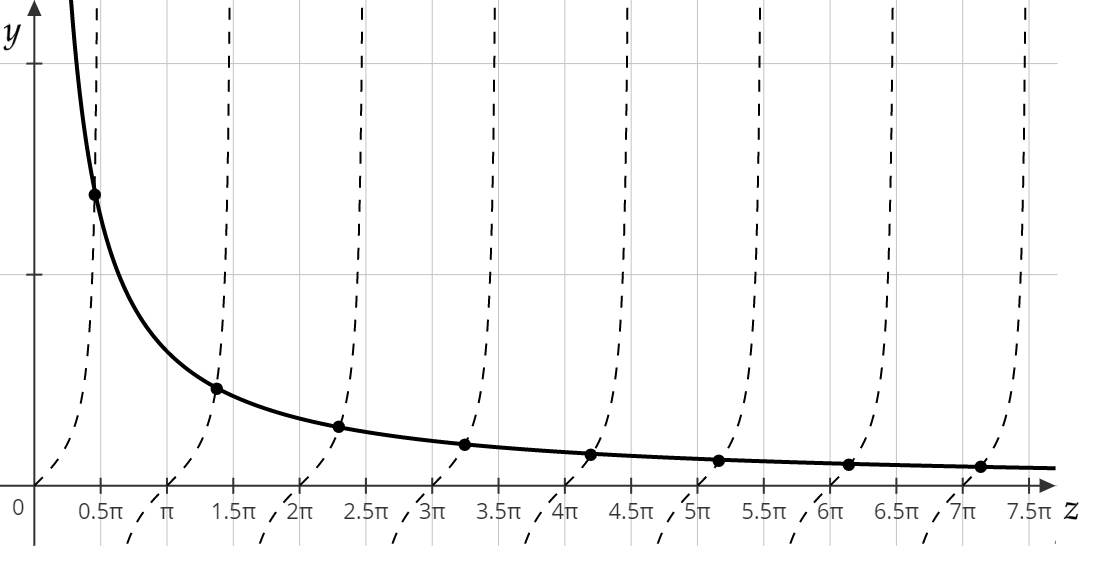
\includegraphics[width=0.7\linewidth]{picture1}
\end{center}
Рисуем графики мы видим, что точки пересечения графиков отвечают всё меньшим значениям $\Tg(z)$, то есть стремятся к $\pi\cdot k$, то есть очевидно, что $|z_k-\pi\cdot  k|\to0$, при $k\to\infty$. Откуда
\begin{equation*}
	\hfill z_k^2=l^2\cdot\omega_k^2=\dfrac{l^2\cdot(\lambda_k-C_2)}{C_1}\geqslant C_0\cdot k^2,\hfill
\end{equation*}	
где $C_0>0$ некоторая константа. Отсюда
\begin{equation*}
	\hfill\lambda_k\geqslant\frac{C_0\cdot C_1}{l^2}\cdot k^2+C_2.\hfill
\end{equation*}
Значит, собственные значения растут со скоростью $k^2$.

Рассмотрим наконец общий случай $\gamma_1\cdot\gamma_2>0$. В этом случае функция $\Psi(z)$ имеет разрыв при $z=z_0=l\cdot\sqrt{\gamma_1\cdot\gamma_2}$, и $\Psi(z_0+0)=+\infty$, $\Psi(z_0-0)=-\infty$.
\begin{center}
	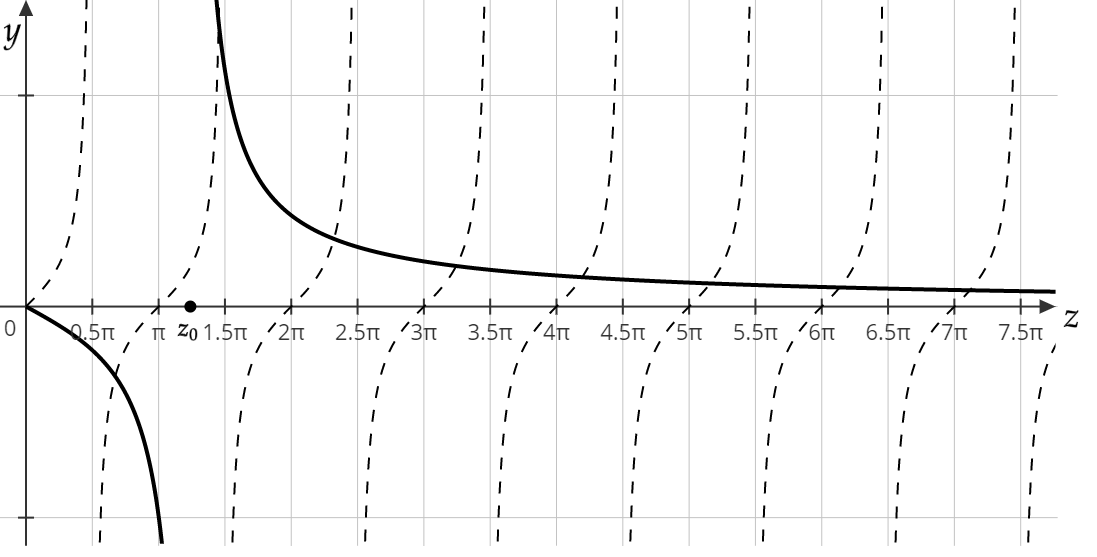
\includegraphics[width=0.7\linewidth]{picture2}
\end{center}
На чертеже $\pi<z_0<\frac{3}{2}\cdot\pi$. Мы видим, что появилась новая точка пересечения на графике $\Psi(z)$ и $\Tg(z)$. В зависимости от положения $z_0$ таких точек или нет --- если $z_0\leqslant{\pi}/{2}$ --- или несколько при $z>{\pi}/{2}$. Пусть слева от $z_0$ имеется $m_0$ решений уравнения~\eqref{l7:eq:11a}, $m_0\geqslant0$ и число $m_1$ таково, что $\pi\cdot m_1\leqslant z_0\leqslant\pi\cdot(m_1+1)$, $m_1\geqslant0$ (связь $m_0$ и $m_1$ нам не интересна). Тогда из графиков $\Tg(z)$ и $\Psi(z)$ видно, что решения $z_{m_0+k}$ будут асимптотически стремиться к $(m_1+k)\cdot\pi$, то есть
\begin{equation*}
	\hfill\displaystyle z_{m_0+k}-\pi\cdot(m_1+k)\to0,\hfill
\end{equation*}
откуда полагая $s=m_0+k$ получаем 
\begin{equation*}
	\hfill z_s-\pi\cdot(m_1-m_0+s)\to0\quad\text{при}\quad s\to\infty\hfill
\end{equation*}
и, значит, 
\begin{equation*}
	\hfill z_s^2=\omega_s^2\cdot l^2=\dfrac{\lambda_s-C_2}{C_1}\geqslant\beta_0\cdot s^2,\quad s\gg1,\hfill
\end{equation*} 
для некоторых $\beta_0>0$, $\beta_0$ не зависит от $s$. Отсюда как и раньше получим
\begin{equation*}
	\hfill\lambda_s\geqslant\beta_1\cdot s^2,\quad s\gg1,\hfill
\end{equation*} 
$\beta_1$ --- некоторая константа. Это означает, что при произвольных $\gamma_1,\,\gamma_2$ собственные значения $\lambda_s$ оператора Штурма с новыми граничными условиями растут при $s\to\infty$ не медленнее (по порядку) чем $s^2$.

Рассмотрим теперь общий случай: оператор Штурма с переменными коэффициентами.
\begin{equation*}
	Ly=-\der{}{x}\Big(Q\cdot y'\Big)+P\cdot y,\quad\mc{D}_{L}^{0}=\left\{y(x)|y\in\Cfn[{[a,b]}]{2},\ y'(a)=\gamma_1\cdot y(a),\,y'(b)=-\gamma_2\cdot y(b),\ \gamma_1\cdot\gamma_2\geqslant0\right\}_{\displaystyle.}
\end{equation*}
Покажем, что оператор Штурма эрмитов в $\mc{D}_{L}^{0}$. Пусть $y(x),\,z(x)\in\mc{D}_{L}^{0}$. Имеем 
\begin{multline}
	\label{l7:eq:12}
	\big(Ly,z\big)=\int\limits_a^b\underbrace{\overline{z}}_{v}\underbrace{\left(-\der{}{x}\Big(Q\cdot y'\Big)\right)\,dx}_{du}+\int\limits_a^b P\cdot y\cdot\overline{z}\,dx=-Q\cdot y'\cdot z\mathop{\Big|}\limits_a^b+\int\limits_a^b\left(Q\cdot y'\cdot\overline{z}'+P\cdot y\cdot\overline{z}\right)\,dx=\\
	=Q(b)\cdot y(b)\cdot\overline{z}(b)\cdot\gamma_2+Q(a)\cdot y(a)\cdot\overline{z}(a)\cdot\gamma_1+\int\limits_a^b\left(Q\cdot y'\cdot\overline{z}'+P\cdot y\cdot\overline{z}\right)\,dx.
\end{multline}
$\big(y,Lz\big)=\overline{\big(Lz,y\big)}$; используем~\eqref{l7:eq:12}, меняя там местами $y$ и $z$ и взяв комплексное сопряжение. Тогда получим, что $\big(Ly,z\big)=\big(y,Lz\big)$. Значит, оператор $L$ в $\mc{D}_{L}^{0}$ эрмитов\footnote{Заметим, кстати, что положительность $\gamma_1$, $\gamma_2$ не используется, а вот вещественность --- нужна.}
\vspace{0.2cm}

\noindent\textbf{Задание.} Доказать, что если $\Im\,\gamma_1\neq0$ или $\Im\,\gamma_2\neq0$, то оператор $L$ --- не эрмитов.
\vspace{0.2cm}

Из эрмитовости оператора $L$ следует, что собственные значения его --- вещественные и что собственные функции, отвечающие различным собственным значениям взаимно ортогональны.

Докажем теперь, что собственные подпространства оператора $L$ --- одномерны. Пусть
\begin{equation*}
	\hfill\Ul=\left\{y(x)|y\in\mc{D}_L^0,\ Ly=\lambda\cdot y\right\}.\hfill
\end{equation*}    
Если $y_1,\,y_2\in\Ul$, то функция $y=C_1\cdot y_1+C_2\cdot y_2\in\Ul$, $\forall C_1,\,C_2\in\mathbb{R}$. Положим
\begin{equation*}
	\hfill y(x)=y_1(x)\cdot y_2(a)-y_2(x)\cdot y_1(a).\hfill
\end{equation*}
Очевидно,
\begin{equation*}
	y(a)=0,\quad y'(a)=y'_1(a)\cdot y_2(a)-y'_2(a)\cdot y_1(a)=\gamma_1\cdot\big(y_1(a)\cdot y_2(a)-y_2(a)\cdot y_1(a)\big)=0.
\end{equation*} 
Так как $Ly=\lambda\cdot y$, то при $Q(a)\neq0$ в силу теоремы единственности получаем $y\equiv0$, поскольку $y_2(a)\neq0$ (иначе $y_2'(a)=0$ и тогда $y_2(x)\equiv0$), то функции $y_1,\,y_2$ линейно зависимы. Значит $\dim\Ul=1$.

Теперь поговорим об экстремальных свойствах собственных значений и собственных функций оператора $L$ в $\mc{D}_L^0$. Вспомним, что при $y(a)=y(b)=0$, то есть в $\mc{D}_L$ 
\begin{equation*}
	\hfill\J[y]=\int\limits_a^b\left(Q\cdot y^{\prime2}+P\cdot y^2\right)\,dx=\big(Ly,y\big)\hfill
\end{equation*} 
и в этом случае экстремальные свойства были связаны с функционалом $\J[y]$. Найдём $\big(Ly,y\big)$ при $y\in\mc{D}_L^0$.

Имеем в силу~\eqref{l7:eq:12} при $z=y$
\begin{equation}
	\label{l7:eq:13}
	\hfill\J_0[y]\eqdef\big(Ly,y\big)=\int\limits_a^b\left(Q\cdot y^{\prime2}+P\cdot y^2\right)\,dx+\gamma_2\cdot y^2(b)\cdot Q(b)+\gamma_1\cdot y^2(a)\cdot Q(a).\hfill
\end{equation} 
Пусть
\begin{equation*}
	\hfill\K=\left\{y(x)|y\in\Cfn[{[a,b]}]{1},\ y'(a)=\gamma_1\cdot y(a),\ y'(b)=-\gamma_2\cdot y(b) \right\}_{\displaystyle.}\hfill
\end{equation*}
Рассмотрим задачу на $\displaystyle\min\limits_{y\in\K}\,\J_0[y]$. 

Функцию $\eta(x)$ назовём допустимым изменением, если $y+t\cdot\eta\in\K$ при $|t|\ll1$, откуда $\eta'(a)={\gamma_1\cdot\eta(a)}$, $\eta'(b)=-\gamma_2\cdot\eta(b)$. Можно взять $\eta'(a)=\eta'(b)=\eta(a)=\eta(b)=0$. Пусть $y$ --- минимайзер для $\J_0$ в $\K$. Тогда как и раньше убеждаемся, что$\displaystyle\left.\der{}{t}\J[y+t\cdot\eta]\right|_{\lefteqn{\scriptstyle t=0}}=0$. Проведём необходимые вычисления, считая что минимайзер обладает повышенной гладкостью, то есть $y\in\Cfn[{[a,b]}]{2}$, ${\eta(x)\in\Cfn[{[a,b]}]{1}}$ и $\eta$ --- не обязательно допустимое изменение. Имеем:
\begin{multline*}
	\left.\der{}{t}\J[y+t\cdot\eta]\right|_{t=0}=\der{}{t}\left\{\int\limits_a^b\Big( Q\cdot(y'+t\cdot\eta')^2+P\cdot(y+t\cdot\eta)^2\Big)\,dx+\gamma_2\cdot Q(b)\cdot\Big(y(b)+t\cdot\eta(b)\Big)^2\right.+\\\left.\left.\vphantom{\int\limits_a^b}+\gamma_1\cdot Q(a)\cdot\Big(y(a)+t\cdot\eta(a)\Big)^2\right\}\right|_{t=0}=2\cdot\int\limits_a^b\Big(Q\cdot y'\cdot\eta'+P\cdot y\cdot\eta\Big)\,dx+2\cdot\gamma_2\cdot Q(b)\cdot y(b)\cdot\eta(b)+\\
	+2\cdot\gamma_1\cdot Q(a)\cdot y(a)\cdot\eta(a)=2\cdot\int\limits_a^b\left(-\der{}{x}\Big(Q\cdot y\Big)+P\cdot y\right)\cdot\eta\,dx+2\cdot Q\cdot y'\cdot\eta\mathop{\Big|}\limits_a^b+\\
	+2\cdot\left[\left.\Big(\gamma_2\cdot Q\cdot y\cdot\eta\Big)\right|_{ x=b}+\left.\Big(\gamma_1\cdot Q\cdot y\cdot\eta\Big)\right|_{ x=a}\right]_{\displaystyle.}
\end{multline*} 
В силу граничных условий вне интегральные члены равны нулю так, что никаких дополнительных граничных условий не возникает, поэтому при допустимых $\eta(x)$
\begin{equation*}
	\hfill\left.\der{}{t}\J_0[y+t\cdot\eta]\right|_{t=0}=\int\limits_a^b\left(-\der{}{x}\Big(Q\cdot y\Big)+P\cdot y\right)\cdot\eta\,dx=0.\hfill
\end{equation*} 
Отсюда в силу леммы Лагранжа мы получаем обычное уравнение Эйлера $Ly=0$. Для нахождения экстремальных свойств собственных функций и собственных значений оператора Штурма в $\mc{D}_L^0$ мы будем рассматривать задачу на минимум $\J_0[y]$ в классе 
\begin{equation*}
	\hfill\K^0\eqdef\left\{y(x)|y\in\Cfn[{[a,b]}]{1},\ y'(a)=\gamma_1\cdot y(a),\;y'(b)=-\gamma_2\cdot y(b),\ \int\limits_a^b y^2\,dx=1\right\}_{\displaystyle.}\hfill
\end{equation*}
Так как задача на $\displaystyle\min\limits_{y\in\K^0}\,\J_0[y]$ --- изопериметрическая, то надо повторить вывод, который мы делали раньше. Если $y$ --- минимайзер, то мы получаем $\tilde{y}=y+\alpha\cdot\eta_1+\beta(\alpha)\cdot\eta_2$, где $\eta_i(a)=\eta_i'(a)=0$, $\eta_i'(b)=\eta_i(b)=0$. Тогда действуя так же, как в случае простейших граничных условий мы получим, что минимайзер в задаче на $\displaystyle\min\limits_{y\in\K^0}\,\J_0[y]$ удовлетворяет уравнению. Эйлера для интегранта $Q\cdot y^{\prime2}+P\cdot y^2-\lambda\cdot y^2$ ($F^{\ast}=F-\lambda\cdot G$) то есть уравнению $Ly=\lambda\cdot y$. После этого доказываем экстремальные свойства собственных значений и собственных функций оператора $L$, а также принцип минимакса, беря всюду $\J_0[y]$ вместо $\J[y]$. После этого доказываем теорему сравнения и с её помощью устанавливаем рост собственных значений $\lambda_k\geqslant C\cdot k^2$ для оператора с переменными $Q(x)$, $P(x)$, после чего доказываем теорему Стеклова, следуя использованной ранее схеме. Советую вам попытаться это сделать. Теперь о практике. Необходимо уметь находить собственные значения и собственные функции с любыми граничными условиями как на левом, так и на правом конце. Приведём эти условия в таблице.
\begin{center}
	\begin{tabular}{|c|c|}
		\hline
		$x=a$ & $x=b$ \\
		\hline
		$y(a)=0$ & $y(b)=0$ \\
		\hline
		$y'(a)=0$ & $y'(b)=0$ \\
		\hline
		$y'(a)=\gamma_1\cdot y(a)$, $\gamma_1>0$ & $y'(a)=-\gamma_2\cdot y(a)$, $\gamma_2>0$ \\
		\hline
	\end{tabular} 
\end{center}

		\chapter{}
\label{lecture8}
\section{Обобщённая задача Штурма.}
\label{lecture8section1}
Мы возвращаемся к простейшим граничным условиям для допустимых функций, но изопериметрическое условие $\smallint\limits_a^b y^2\,dx=1$ мы заменим более общим. Итак
\begin{equation*}
	\J[y]=\int\limits_a^b\Big(Q\cdot y^{\prime2}+P\cdot y^2\Big)\,dx,\quad\K=\left\{y(x)|y\in\Cfn[{[a,b]}]{1},\ y(a)=y(b)=0,\ \int\limits_a^b\rho\cdot y^2\,dx=1\right\},
\end{equation*}
где $\rho(x)>0$ при $x\in(a,b]$ ---  некоторая непрерывная на $[a,b]$ функция. При $\rho(a)=0$ мы всегда считаем, что $P(x)\geqslant 0$, $x\in[a,b]$, иначе был бы возможен случай, когда $\displaystyle\inf\limits_{y\in\mc{K}}\J[y]=-\infty$; попробуйте привести пример такой ситуации. Ищем $\displaystyle\min\limits_{y\in\K}\,\J[y]$. Составляем $F^{*}=F-\lambda\cdot G=Q\cdot y^{\prime2}+P\cdot y^2-\lambda\cdot\rho\cdot y^2$ и пишем для $F^{*}$ уравнение Эйлера. Получим	
\begin{equation}
	\label{l8:eq:1}
	\hfill P\cdot y-\der{}{x}\Big(Q\cdot y'\Big)-\lambda\cdot\rho\cdot y=0\quad\text{или}\quad Ly=\lambda\cdot\rho\cdot y\hfill
\end{equation}

Оператор $L$ рассматривается в $\mc{D}_L\eqdef\left\{y(x)|y\in\Cfn[{[a,b]}]{2},\ y(a)=y(b)=0\right\}$. Функция удовлетворяющая~\eqref{l8:eq:1}, называется собственной функцией обобщённой задачи Штурма, а $\lambda$ --- собственным значением этой задачи. Так как оператор $L$ --- эрмитов, то 
\begin{equation*}
	\hfill\big(Ly,y\big)=\big(y,Ly\big)=\overline{\big(Ly,y\big)}.\hfill
\end{equation*}
Значит, число $\big(Ly,y\big)$ --- вещественно и поэтому из~\eqref{l8:eq:1} следует вещественность собственного значения $\lambda$ обобщённой задачи Штурма:
\begin{equation}
	\label{l8:eq:2}
	\hfill\big(Ly,y\big)=\lambda\cdot\big(\rho\cdot y,y\big)\quad\Rightarrow\quad\lambda=\big(Ly,y\big)\!\Bigm/\!\big(\rho\cdot y,y\big)\text{ --- вещественно.}\hfill
\end{equation}

Далее, собственные функции обобщённой задачи Штурма, отвечающие различным собственным значениям, ортогональны с весом $\rho$. 
\begin{proof}
	Действительно, если $Ly_1=\lambda_1\cdot\rho\cdot y_1$, $Ly_2=\lambda_2\cdot\rho\cdot y_2$ и $\lambda_2\neq\lambda_1$, то, умножая первое соотношение на $y_2$ скалярно, получим $\big(Ly_1,y_2\big)=\lambda_1\cdot\big(\rho\cdot y_1,y_2\big)$ и одновременно
	\begin{equation}
		\label{l8:eq:3}
		\hfill\big(Ly_1,y_2\big)=\big(y_1,Ly_2\big)=\big(y_1,\lambda_2\cdot\rho\cdot y_2\big)=\lambda_2\cdot\big(y_1,\rho\cdot y_2\big).\hfill
	\end{equation}	
	Отсюда
	\begin{equation}
		\hfill(\lambda_2-\lambda_1)\cdot\big(y_1,\rho\cdot y_2\big)=0\quad\Rightarrow\quad\big(y_1,\rho\cdot y_2\big)=0.\hfill
	\end{equation}
\end{proof}

Пусть\  $\Ul=\left\{y(x)|y\in\mc{D}_L,\ Ly=\lambda\cdot\rho\cdot y\right\}$ --- собственное подпространство для обобщённой задачи Штурма. Точно так же как и в обычной задаче Штурма, доказывается, что $\dim\Ul=1$, то есть собственные значения обобщённой задачи Штурма --- не вырождены и, значит, каждому $\lambda$ отвечает одна (с точностью до знака) собственная функция обобщённой задачи Штурма, удовлетворяющая изопериметрическому условию $\smallint\limits_a^b\rho\cdot y^2\,dx=1$.

Далее введём пространство функций \fLr\ интегрируемых с весом $\rho$, $\rho(x)>0$ $x\in(a,b]$, $\rho(x)\in\Cfn[{[a,b]}]{}$:
\begin{equation*}
	\hfill\fLr\eqdef\left\{y(x)\middle| \int\limits_a^b\rho|y|^2\,dx<+\infty\right\}_{\displaystyle.}\hfill
\end{equation*}
Если $\rho(a)=0$, то $\fLr\supset\fL$ (приведите обоснование!), если $\displaystyle\inf\limits_{x\in[a,b]}\rho(x)>0$, то $\fLr\?=\fL$. В пространстве \fLr\ введём скалярное произведение и норму
\begin{equation*}
	\hfill\big(u(x),v(x)\big)_1\eqdef\int\limits_a^b\rho\cdot u\cdot\overline{v}\,dx=\big(u,\rho\cdot v\big),\quad{\norm{u}}_1^2\eqdef\big(u,u\big)_1.\hfill
\end{equation*}
Таким образом класс $\K$ запишется так:
\begin{equation*}
	\hfill\K=\left\{y(x)|y\in\Cfn[{[a,b]}]{1},\ y(a)=y(b)=0,\ \norm{y}_1=1\right\},\hfill
\end{equation*}
а условие ортогональности с весом $\left\{\big(u,\rho\cdot v\big)=0\right\}\sim\left\{\big(u,v\big)_1=0\right\}$. Таким образом, если $Ly_1\?=\lambda_1\cdot\rho\cdot y_1$, $Ly_2=\lambda_2\cdot\rho\cdot y_2$, $y_i\in\mc{D}_L$ и $\lambda_1\neq\lambda_2$, то $\big(y_1,y_2\big)_1=0$.

Далее устанавливаем экстремальные свойства собственных значений и собственных функций обобщённой задачи Штурма. При этом используем соотношения $\big(Ly,y\big)=\J[y]$ и $\big(Ly,y\big)=\lambda$, если $Ly=\lambda\cdot\rho\cdot y$ и $\norm{y}_1=1$. Тогда $\displaystyle\inf\limits_{y\in\K}\,\J[y]$ --- наименьшее собственное значение обобщённой задачи Штурма, а минимайзер $y_1$ этой задачи --- соответствующая собственная функция. Далее $\displaystyle\inf\limits_{\substack{y\in\K,\\ \scriptstyle{(y,y_1)}_1=0}}\,\J[y]$ --- второе по величине собственное значение обобщённой задачи Штурма и так далее. Доказательство практически полностью повторяет приведённое для стандартной задачи Штурма.

Далее для обобщённой задачи Штурма устанавливается принцип минимакса. Это делается так же, как раньше, только вместо $\norm{\phantom{x}}$ надо брать $\norm{\phantom{x}}_1$; вместо условия ортогональности $\big(\cdot\,,\cdot\big)=0$ надо брать $\big(\cdot\,,\cdot\big)_1=0$, и вместо $\phi_j\in\fL$ надо брать $\phi_j\in\fLr$. После этого устанавливаем теорему сравнения. Она устанавливается так же, как и раньше: если 
\begin{equation*}
	\hfill L_iy=-\der{}{x}\Big(Q_i\cdot y'\Big)+P_i\cdot y,\ i=1,2\text{ и }L_1y_k^{(1)}=\lambda_k^{(1)}\cdot\rho\cdot y_k^{(1)},\ L_2y_k^{(2)}=\lambda_k^{(2)}\cdot\rho\cdot y_k^{(2)},\hfill
\end{equation*} 
то при $Q_1\geqslant Q_2$, $P_1\geqslant P_2$ выполняется $\lambda_k^{(1)}\geqslant\lambda_k^{(2)}$. Обратите внимание, что для обоих операторов сравнения $\rho$ --- \emph{одно и то же}.

В случае обычной задачи Штурма мы брали $\displaystyle Q_2=\min\limits_{x\in[a,b]}Q_1(x)$, $\displaystyle P_2=\min\limits_{x\in[a,b]}P_1(x)$ и получали оператор $L_2$ с постоянными коэффициентами, для которого было известно, что собственные значения $\lambda_k^{(2)}$ растут со скоростью $k^2$ ($\rho=1$!).

В случае обобщённой задачи Штурма мы не можем найти собственные значения $\lambda_k^{(2)}$ даже при постоянных $P_2$ и $Q_2$, из-за наличия  функции $\rho(x)$. Поэтому нам понадобится ещё одна теорема сравнения.

Прежде чем её формулировать рассмотрим пример, подсказывающий какое поведение собственных значений обобщённой задачи Штурма можно ожидать при росте $\rho(x)$. Пусть $\lambda_k$ и $y_k$, $k=1,2,\ldots$ --- собственные значения и собственные функции оператора Штурма:
\begin{equation*}
	L y_k=\lambda_k\cdot y_k.
\end{equation*}
Для $\forall d_1>0$ очевидно
\begin{equation*}
	L y_k=\lambda_k(d_1)\cdot d_1\cdot y_k,
\end{equation*}
где $\lambda_k(d_1)=\lambda_k/d_1$. Поэтому $\lambda_k(d_1)$ можно рассматривать как $k$-ое собственное значение обобщённой задачи Штурма с $\rho(x)=d_1$. Аналогично при $d_2\geqslant d_1$ имеем 
\begin{equation*}
	L y_k=\lambda_k(d_2)\cdot d_2\cdot y_k,
\end{equation*}
где $\lambda_k(d_2)=\lambda_k/d_2$. Так как $d_2\geqslant d_1$, то при положительных $\lambda_k$
\begin{equation*}
	\lambda_k(d_2)\leqslant\lambda_k(d_1)\quad\text{при }d_2\geqslant d_1.
\end{equation*}
Это неравенство и есть подсказка возможного поведения собственных значений обобщённой задачи Штурма при росте $\rho(x)$.

\begin{_teor}[вторая теорема сравнения]\label{l8:teor:8.1}
	Пусть $\lambda_k^{(i)}$; $k=1,2,\ldots$; $i=1,2$ --- собственные значения двух обобщённых задач Штурма с одним и тем же оператором $L$  и с разными $\rho(x)$:
	\begin{equation*}
		Ly_k^{(i)}=\lambda_{k}^{(i)}\cdot\rho_i(x)\cdot y_k^{(i)};\quad k=1,2,\ldots;\ i=1,2
	\end{equation*}
	и пусть 
	\begin{equation*}
		\J[y]\eqdef\big(L y,y\big)\geqslant0,\ y\in\mc{D}_{L},\quad\sup\limits_{x\in[a,b]}\frac{\rho_2(x)}{\rho_1(x)}<+\infty.
	\end{equation*}
	Тогда если $\rho_2(x)\geqslant\rho_1(x)$, то
	\begin{equation}\label{l8:eq:1.5}
		\lambda_k^{(2)}\leqslant\lambda_k^{(1)},\quad k=1,2,\ldots
	\end{equation}
\end{_teor}
Для доказательства теоремы нам понадобится 
\begin{_lemm}\label{l8:lemm:8.1}
	Положим 
	\begin{equation*}
		M_{ij}=\frac{\rho_i(x)}{\rho_j(x)},\quad A_1=\left\{M_{12}\cdot\phi(x)|\forall\phi\in\fLr[{[a,b];\rho_1}]\right\},\quad A_2=\fLr[{[a,b];\rho_2}]
	\end{equation*}
	и пусть 
	\begin{equation*}
		\overline{M}_{ij}=\max\limits_{x\in[a,b]}M_{ij}(x)<+\infty,\quad i,j=1,2.
	\end{equation*}
	Тогда
	\begin{equation*}
		A_1=A_2.
	\end{equation*}
\end{_lemm}
\begin{proof}[Доказательство леммы~\ref{l8:lemm:8.1}.]
	Пусть $\psi\in A_2$ и $\phi=M_{21}\cdot\psi$. Очевидно, $M_{12}\cdot\phi=\psi$ и 
	\begin{equation*}
		\norm{\phi}_1^2=\int\limits_{a}^{b}M_{21}^2\cdot|\psi|^2\cdot\rho_1\,dx=\int\limits_{a}^{b}M_{21}\cdot|\psi|^2\cdot\rho_2\,dx\leqslant\overline{M}_{21}\cdot\norm{\psi}_2^2<+\infty.
	\end{equation*}
	Значит, $\phi\in\fLr[{[a,b];\rho_1}]$ и поэтому $\psi=M_{12}\cdot\phi\in A_1$. Следовательно
	\begin{equation*}
		A_2\subseteq A_1.
	\end{equation*}

	Рассмотрим теперь $\psi=M_{12}\cdot\phi\in A_1$ и покажем, что $\psi\in A_2$. Имеем
	\begin{equation*}
		\norm{\psi}_2^2=\int\limits_a^b M_{12}^2\cdot|\phi|^2\cdot\rho_2\,dx=\int\limits_a^b M_{12}\cdot|\phi|^2\cdot\rho_1\,dx\leqslant\overline{M}_{12}\cdot\norm{\phi}_1^2<+\infty.
	\end{equation*}
	Значит, $\psi\in A_2$ и поэтому 
	\begin{equation*}
		A_1\subseteq A_2.
	\end{equation*}
	Но раньше мы получили, что $A_2\subseteq A_1$, следовательно
	\begin{equation*}
		A_1=A_2
	\end{equation*}
	и \emph{лемма~\ref{l8:lemm:8.1} доказана.}
\end{proof}
\begin{_rem}
	Если $\rho_1>0$, $\rho_2(x)>0$, $x\in[a,b]$, то $\overline{M}_{ij}<+\infty$, $i,j=1,2$.
\end{_rem}
\begin{proof}[Доказательство теоремы~\ref{l8:teor:8.1}.]
	Пусть
	\begin{equation*}
		T=\left\{y(x)|y\in\Cfn[{[a,b]}]{1},\;y(a)=y(b)=0\right\}
	\end{equation*}
	и $y\in T$. Тогда так как $\norm{y}_2\geqslant\norm{y}_1$, то 
	\begin{equation}\label{l8:eq:1.6}
		\J[y]\cdot\norm{y}_2^{-2}\leqslant\J[y]\cdot\norm{y}_1^{-2}.
	\end{equation}
	Пусть далее $\phi_i(x)$, $i=\overline{1,n}$ --- произвольные фиксированные функции из $\fLr[{[a,b];\rho_1}]$ и $\big(y,\phi_i\big)_1=0$, $i=\overline{1,n}$. Положим $\psi_i=M_{12}\cdot\phi_i$. Так как
	\begin{equation*}
		\big(y,\phi_i\big)_1=\big(y,\rho_1\cdot\phi_i\big)=\big(y,M_{12}\cdot\rho_2\cdot\phi_i\big)=\big(y,\psi_i\big)_2,
	\end{equation*}
	то условие $\big(y,\phi_i\big)_1=0$ эквивалентно условию $\big(y,\psi_i\big)_2=0$ при $\psi_i=M_{12}\cdot\phi_i$. При фиксированных $y$ и $\phi_i$, $i=\overline{1,n}$ возьмём в левой части~\eqref{l8:eq:1.6} минимум по всем $\widetilde{y}\in T$, $\big(\widetilde{y},\psi_i\big)_2=0$, $i=\overline{1,n}$. Получим
	\begin{equation}\label{l8:eq:1.6a}
		\nu_2(\psi_1,\ldots,\psi_n)\eqdef\min\limits_{\substack{\widetilde{y}\in T,\\\lefteqn{\scriptstyle \hspace*{-0.8cm}(\widetilde{y},\psi_i)_2=0,\:i=\overline{1,n}}}}\J[\widetilde{y}]\leqslant\J[y]\cdot\norm{y}_1^{-2}. \tag{\theequation a}
	\end{equation}
	Теперь в правой части~\eqref{l8:eq:1.6a} возьмём минимум по всем $y\in T$, $\big(y,\phi_i\big)_1=0$, $i=\overline{1,n}$. Тогда в силу~\eqref{l8:eq:1.6a}
	\begin{equation*}
		\nu_2(\psi_1,\ldots,\psi_n)\leqslant\nu_1(\phi_1,\ldots,\phi_n)\eqdef\min\limits_{\substack{{y}\in T,\\\lefteqn{\scriptstyle \hspace*{-0.8cm}(y,\phi_i)_1=0,\:i=\overline{1,n}}}}\J[y]\cdot\norm{y}_1^{-2}.
	\end{equation*}
	Таким образом мы доказали неравенство
	\begin{equation}\label{l8:eq:1.6b}
		\nu_2(\psi_1,\ldots\psi_n)\leqslant\nu_1(\phi_1,\ldots,\phi_n)\tag{\theequation b}
	\end{equation}
	которое верно при $\forall\phi_i\in\fLr[{[a,b];\rho_1}]$ и $\psi_i=M_{12}\cdot\phi_i$, $i=\overline{1,n}$. Возьмём в правой части~\eqref{l8:eq:1.6b} максимум по всем $\widetilde{\phi}_i\in\fLr[{[a,b];\rho_1}]$ при фиксированных слева $\psi_i=M_{12}\cdot\phi_i$. Получим
	\begin{equation}\label{l8:eq:1.6c}
		\nu_2(\psi_1,\ldots,\psi_n)\leqslant\max\limits_{\lefteqn{\vphantom{\big(}\scriptstyle \widetilde{\phi}_1,\ldots,\widetilde{\phi}_n\in\fLr[{[a,b];\rho_1}]}}\nu_1(\widetilde{\phi}_1,\ldots,\widetilde{\phi}_n).\tag{\theequation c}
	\end{equation}
	Так как данное неравенство верно при $\forall\phi_i\in\fLr[{[a,b];\rho_1}]$ и так как $\psi_i=M_{12}\cdot\phi_i$, то мы можем слева в~\eqref{l8:eq:1.6c} взять максимум по всем $\phi_i$, но в силу леммы~\ref{l8:lemm:8.1} когда набор $\phi_1,\ldots,\phi_n$ будет пробегать все системы $n$ функций из $\fLr[{[a,b];\rho_1}]$, то набор $\psi_1,\ldots,\psi_n$ будет пробегать все системы $n$ функций из $\fLr[{[a,b];\rho_2}]$, поэтому слева в~\eqref{l8:eq:1.6c} мы можем взять максимум по всем системам $\widetilde{\psi}_1,\ldots,\widetilde{\psi}_n$ из $\fLr[{[a,b];\rho_2}]$. Получим
	\begin{equation}\label{l8:eq:1.6d}
		\max\limits_{\lefteqn{\vphantom{\big(}\scriptstyle \widetilde{\psi}_1,\ldots,\widetilde{\psi}_n\in\fLr[{[a,b];\rho_2}]}}\nu_2(\widetilde{\psi}_1,\ldots,\widetilde{\psi}_n)\leqslant\max\limits_{\lefteqn{\vphantom{\big(}\scriptstyle \widetilde{\phi}_1,\ldots,\widetilde{\phi}_n\in\fLr[{[a,b];\rho_1}]}}\nu_1(\widetilde{\phi}_1,\ldots,\widetilde{\phi}_n).\tag{\theequation d}
	\end{equation}
	В силу принципа минимакса~\eqref{l8:eq:1.6d} --- это и есть доказываемое неравенство~\eqref{l8:eq:1.5}.
\end{proof}

Применим теорему~\ref{l8:teor:8.1}, считая $\overline{M}_{21}<+\infty$ и взяв $\rho_2=\max\limits_{x\in[a,b]}\rho_1(x)$. Тогда обобщённая задача Штурма
\begin{equation*}
	L y_k^{(2)}=\lambda_{k}^{(2)}\cdot\rho_2\cdot y_k^{(2)}
\end{equation*}
превращается в обычную задачу Штурма для оператора $L/\rho_2$. А для этого оператора мы знаем, что $\exists c_0>0$ так, что 
\begin{equation*}
	\lambda_k^{(2)}\geqslant c_0\cdot k^2,\quad k\gg1.
\end{equation*}
В силу~\eqref{l8:eq:1.5} получаем
\begin{equation}\label{l8:eq:1.7}
	\lambda_k^{(1)}\geqslant c_0\cdot k^2,\quad k\gg1.
\end{equation}
Совершенно аналогично можно установить неравенство 
\begin{equation}\label{l8:eq:1.7a}
	\lambda_{k}^{(2)}<c_1\cdot k^2,\tag{\theequation a}
\end{equation}
если взять $\rho_1=\min\limits_{x\in[a,b]}\rho_2(x)$ при $\rho_1>0$.
%, которую я привожу без доказательства. Смысл её: увеличение $\rho(x)$ уменьшает собственные значения обобщённой задачи Штурма. Теперь точная формулировка.
%\begin{_teor}[вторая теорема сравнения]\label{l8:teor:1.1}
%	Пусть
%	\begin{equation}\label{l8:eq:5}
%		\hfill Q_3\leqslant Q_1,\quad P_3\leqslant P_1,\quad\rho_3\geqslant\rho_1\geqslant0\quad\text{и}\quad L_3y_k^{(3)}=-\der{}{x}\Big(Q_3\cdot {y_k^{(3)}}'\Big)+P_3\cdot y_k^{(3)}=\lambda_k^{(3)}\cdot\rho_3\cdot y_k^{(3)}.\hfill
%	\end{equation}
%	Тогда при $\lambda^{(3)}_k>0$ 
%	\begin{equation}\label{l8:eq:6}
%		\hfill\lambda_k^{(3)}\leqslant\lambda_k^{(1)}.\hfill
%	\end{equation}
%\end{_teor}
%
%Взяв $Q_3=\displaystyle\min\limits_{x\in[a,b]}Q_1(x)$, $P_3=\displaystyle\min\limits_{x\in[a,b]}P_1(x)$, $\rho_3=\displaystyle\max\limits_{x\in[a,b]}\rho(x)$ и поделив~\eqref{l8:eq:1.5} на $\rho_3$ мы получим, что числа $\lambda_k^{(3)}$ --- собственные значения оператора Штурма с постоянными коэффициентами --- $\sfrac{Q_3}{\rho_3}$, $\sfrac{P_3}{\rho_3}$. Значит для некоторой константы $C>0$ при $k\gg1$ выполняется  $\lambda_k^{(3)}\geqslant C\cdot k^2$ и в силу~\eqref{l8:eq:1.6} 
%\begin{equation}\label{l8:eq:7}
%	\hfill\lambda_k^{(1)}\geqslant C\cdot k^2\hfill
%\end{equation}

В силу~\eqref{l8:eq:1.7},~\eqref{l8:eq:1.7a} собственные значения обобщённой задачи Штурма растут со скоростью $k^2$ при росте $k$.

%\noindent\textbf{Замечание} к теореме сравнения собственных значений обобщённой задачи Штурма при росте веса $\rho$. Пусть $\rho\geqslant0$, $d>0$ --- любое число.
%\begin{equation*}
%	\hfill Ly_k=\lambda_k\cdot\rho\cdot y_k,\hfill
%\end{equation*}
%где $\lambda_k$ и $y_k$ соответственно $k$-ое собственное значение и отвечающая ему собственная функция обобщённой задачи Штурма. Предполагаем, что $\lambda_k>0$.
%
%Пусть $\rho_d\eqdef d\cdot\rho$, $\lambda_k(d)\eqdef\lambda_k/d$. Тогда 
%\begin{equation*}
%	\hfill Ly_k=\rho_d\cdot\lambda_k(d)\cdot y_k,\hfill
%\end{equation*}
%то есть для нового веса $\rho_d=d\cdot\rho$ оператор $L$ будет иметь те же собственные функции, что и раньше, но они будут отвечать другим собственным значениям $\lambda_k(d)=\lambda_k/d$. Мы видим, что при $d>1$, $\rho_d>\rho$, а $\lambda_k(d)<\lambda_k$. И вообще, если $d_2>d_1$, то $\rho_{d_2}>\rho_{d_1}$, а $\lambda_k(d_2)<\lambda_k(d_1)$.
%
%Разумеется, этот пример \emph{ничего не доказывает}, но он показывает, почему при росте веса $\rho$ собственные значения уменьшаются.

Все эти результаты получены при условии $\J[y]\geqslant0$ при $y\in\mc{D}_{L}$, то есть при неотрицательности всех собственных значений обобщённой (и обычной!) задачи Штурма. Рассмотрим теперь случай, когда 
\begin{equation*}
	\beta\eqdef\inf\limits_{i\in\K}\J[y]<0.
\end{equation*} 
Пусть $\alpha>-\beta$ и 
\begin{equation*}
	L(\alpha)y=Ly+\alpha\cdot\rho\cdot y.
\end{equation*}
Тогда 
\begin{equation*}
	\J^{(\alpha)}(y)\eqdef\big(L(\alpha)y,y\big)=\big(Ly,y\big)+\alpha\cdot\big(\rho\cdot y,y\big)=\J[y]+\alpha\cdot\norm{y}_1^2>0.
\end{equation*}
Следовательно, собственные значения $\lambda_k(\alpha)$ обобщённой задачи Штурма для оператора $L(\alpha)$ стремятся к $+\infty$ при $k\to\infty$ со скоростью $c_3\cdot k^2$, где $c_3>0$ --- некоторая константа. Так как для исходной задачи Штурма 
\begin{equation*}
	L y_k=\lambda_k\cdot\rho\cdot y_k,
\end{equation*}
то 
\begin{equation*}
	L(\alpha)y_k=L y_k+\alpha\cdot\rho\cdot y_k=\lambda_k\cdot\rho\cdot y_k+\alpha\cdot\rho\cdot y_k=(\lambda_k+\alpha)\cdot\rho\cdot y_k.
\end{equation*}
Значит,
\begin{equation*}
	\lambda_k(\alpha)=\lambda_k+\alpha
\end{equation*}
и, следовательно $\lambda_k\to+\infty$ со скоростью $c_3\cdot k^2$.

Если $\rho(x)>0$, $x\in[a,b]$ и $\rho(x)\in\Cfn[{[a,b]}]{2}$, то можно обойтись без теоремы сравнения~\ref{l8:teor:8.1} следующим образом. Пусть
\begin{equation}\label{l8:eq:8}
	\hfill L_1y_k\eqdef-\der{}{x}\Big(Q_1\cdot y'_k\Big)+P_1\cdot y_k=\lambda_k^{(1)}\cdot\rho_1\cdot y_k.\hfill
\end{equation}
Вводим фкнкцию $z_k\eqdef\sqrt{\rho_1}\cdot y_k$ и поделим обе части~\eqref{l8:eq:8} на $\sqrt{\rho_1}$. Тогда полученное уравнение можно записать в виде
\begin{equation}\label{l8:eq:9}
	\hfill L_0z_k\eqdef-\der{}{x}\Big(Q_0\cdot z'_k\Big)+P_0\cdot z_k=\lambda_k^{(1)}\cdot z_k,\hfill
\end{equation}
где $\displaystyle Q_0=\frac{Q_1}{\rho_1}$, $\displaystyle P_0=\frac{P_1}{\rho_1}+\frac1{\sqrt{\rho_1}}\cdot\der{}{x}\left(\frac12\cdot\frac{Q_1\cdot\rho'_1}{\rho_1^{\sfrac{3}{2}}}\right)$.

Таким образом, собственные значения $\lambda_k^{(1)}$ оператора $L_1$ обобщённой задачи Штурма совпадают с собственными значениями оператора $L_0$ обычной задачи Штурма. Отсюда следует рост собственных значений $\lambda_k^{(1)}$ со скоростью $k^2$ при $k\to\infty$. Далее можно сформулировать и доказать неравенство Бесселя и равенство Парсеваля, а также определить понятие полной системы. Разумеется при этом надо обобщённые коэффициенты Фурье считать с помощью скалярного произведения $\big(\cdot\,,\cdot\big)_1$ и вместо $\norm{\,\cdot\,}$ брать $\norm{\,\cdot\,}_1$.

Далее можно передоказать теорему Стеклова, но в предположении, что $\rho(x)>0$, $x\in[a,b]$. Наметим основные формулировки. Пусть $y\in\fLr$, $y_k$ --- собственные функции обобщённой задачи Штурма, $\norm{y_k}_1=1$, $k=1,2,\ldots$,
\begin{equation*}
	\hfill C_k=\big(y,y_k\big)_1,\quad S_n=\sum\limits_{k=1}^n C_k\cdot y_k,\quad R_n=y-S_n.\hfill
\end{equation*}
\begin{_teor}[Стеклова]\hfill
	\begin{enumerateP1}
		\item\label{l8:Steclov:p1} Для $\forall y\in\fLr$ выполняется $\norm{y-S_n}_1\to0$ при $n\to\infty$, то есть
		\begin{equation*}
			\hfill\int\limits_a^b\left|y-\sum\limits_{k=1}^n C_k\cdot y_k\right|^2\cdot\rho(x)\,dx\to0,\quad\text{при}\quad n\to\infty.\hfill
		\end{equation*}
		(Это сходимость в среднем с весом $\rho$.)
		
		\item\label{l8:Steclov:p2} Для $y\in\mc{D}_L$
		\begin{equation*}
			\hfill\sup\limits_{x\in[a,b]}\left|y(x)-\sum\limits_{k=1}^{n}C_k\cdot y_k\right|\to0,\quad\text{при}\quad n\to\infty.\hfill
		\end{equation*}
		(Это равномерная сходимость.)
	\end{enumerateP1}
\end{_teor}
\noindent Доказательство~\ref{l8:Steclov:p2} я приведу прямо сейчас,~\ref{l8:Steclov:p1} --- без доказательства.

В заключение отметим, что если $0<\underline{\rho}\leqslant\rho(x)\leqslant\overline{\rho}$ для $\forall x\in[a,b]$, где $\underline{\rho}$, $\overline{\rho}$ --- константы, то 
\begin{equation*}
	\hfill\underline{\rho}\cdot\norm{y-S_n}^2\leqslant\norm{y-S_n}_1^2\leqslant\overline{\rho}\cdot\norm{y-S_n}^2,\hfill
\end{equation*}
то есть из сходимости обобщённого ряда Фурье в метрике $\norm{\,\cdot\,}_1$ следует сходимость в метрике $\norm{\,\cdot\,}$ и наоборот. Разумеется здесь в сумме $S_n$ имеем $C_k=\big(y,y_k\big)_1$ не зависимо от того, берётся ли норма $\norm{\,\cdot\,}_1$ или $\norm{\,\cdot\,}$.
\begin{proof}[Теорема Стеклова для собственных функций обобщённой задачи Штурма.]\hfill\\
	Мы будем следовать схеме доказательства теоремы Стеклова, которую мы рассматривали раньше. Пусть
	\begin{gather*}
		y_k\in\mc{D}_L,\quad y_k:\,Ly_k=\lambda_k\cdot \rho\cdot y_k,\quad\big(Ly,y\big)=\lambda\cdot\norm{y}_1^2=\J[y].\\
		S_n=\sum\limits_{k=1}^n C_k\cdot y_k,\quad C_k=\big(y,y_k\big)_1,\quad R_n=y-S_n,\quad \widetilde{R}_n=\dfrac{R_n}{\norm{R_n}_1}.
	\end{gather*}
	Так как
	\begin{equation*}
		\big(\widetilde{R}_n,y_j\big)_1=0,\ j=\overline{1,n}\quad\Rightarrow\quad\widetilde{R}_n\in\K_{n+1}\quad\Rightarrow\quad\J[\widetilde{R}_n]\geqslant\lambda_{n+1}\quad\Rightarrow\quad\J[R_n]\geqslant\lambda_{n+1}\cdot\norm{R_n}^2_1.
	\end{equation*}
	Если $\sup\limits_{n}\,\J[R_n]<+\infty$, то из неравенства (верного при $n\gg1\ \Rightarrow\ \lambda_{n+1}>0$)
	\begin{equation*}
		\hfill\frac{\J[R_n]}{\lambda_{n+1}}\geqslant\norm{R_n}_1\quad\Rightarrow\quad\norm{R_n}_1\to0,\text{ при }n\to\infty.\hfill
	\end{equation*}
	Оценим 
	\begin{equation*}
		\J[R_n]=\big(LR_n,R_n\big)=\big(Ly-LS_n,y-S_n\big)=\big(Ly,y\big)+\big(LS_n,S_n\big)-\big(Ly,S_n\big)-\big(LS_n,y\big).
	\end{equation*}
	\begin{multline*}
		\underline{\big(LS_n,S_n\big)}=\left(\sum\limits_{k=1}^n C_k\cdot Ly_k,\sum\limits_{m=1}^n C_m\cdot y_m\right)=\sum\limits_{k,m=1}^n C_k\cdot\overline{C}_m\cdot\big(\rho\cdot\lambda_k\cdot y_k,y_m\big)=\\
		=\sum\limits_{k,m=1}^n C_k\cdot\overline{C}_m\cdot\lambda_k\cdot\underbrace{\big(\rho\cdot y_k,y_m\big)}_{\textstyle=\big(y_k,y_m\big)_1}=\sum\limits_{k,m=1}^n C_k\cdot\overline{C}_m\cdot\lambda_k\cdot\delta_{km}=\sum\limits_{k=1}^n\lambda_k\cdot|C_k|^2
	\end{multline*}
	Далее
	\begin{gather*}
		\underline{\big(LS_n,y\big)}=\left(\sum\limits_{k=1}^n C_k\cdot Ly_k,y\right)=\sum\limits_{k=1}^nC_k\cdot\big(\lambda_k\cdot\rho\cdot y_k,y\big)=\sum\limits_{k=1}^n C_k\cdot\lambda_k\underbrace{\big(\rho\cdot y_k,y\big)}_{\textstyle=\overline{C}_k}=\sum\limits_{k=1}^n\lambda_k\cdot|C_k|^2\\
		\underline{\big(Ly,S_n\big)}=\big(y,LS_n\big)=\overline{\big(LS_n,y\big)}=\sum\limits_{k=1}^n\lambda_k\cdot|C_k|^2
	\end{gather*}
	
	В силу этих равенств
	\begin{equation*}
		\hfill\J[R_n]=\big(Ly,y\big)-\sum\limits_{k=1}^n\lambda_k\cdot|C_k|^2.\hfill
	\end{equation*}
	Так как $\lambda_k\to\infty$, то $\exists n_0$, $\lambda_k>0$ при $k>n_0$. Тогда, взяв $n>n_0$, получим 
	\begin{equation*}
		\hfill\J[R_n]=\big(Ly,y\big)-\sum\limits_{k=1}^{n_0}\lambda_k\cdot|C_k|^2-\sum\limits_{k=n_0+1}^n\lambda_k\cdot|C_k|^2\leqslant\big(Ly,y\big)-\sum\limits_{k=1}^{n_0}\lambda_k\cdot|C_k|^2=\J[R_{n_0}],\hfill
	\end{equation*}
	и, значит, 
	\begin{equation*}
		\hfill\sup\limits_{n}\J[R_n]<+\infty,\hfill
	\end{equation*}
	и поэтому в силу вышесказанного 
	\begin{equation*}
		\hfill\norm{R_n}_1\to0.\hfill
	\end{equation*}
	
	Докажем теперь равномерную сходимость обобщённого ряда Фурье $\displaystyle\sum\limits_{k=1}^{\infty}C_k\cdot y_k$. Оценим $C_k$.
	\begin{equation*}
		|C_k|=\big|\big(y,\rho\cdot y_k\big)\big|=\left|\left(y,\frac{Ly_k}{\lambda_k}\right)\right|=\frac1{|\lambda_k|}\cdot\big|\big(Ly,y_k\big)\big|\leqslant\frac1{|\lambda_k|}\cdot\left|\left(\frac{Ly}{\rho},\rho\cdot y_k\right)\right|=\frac1{|\lambda_k|}\cdot d_k,
	\end{equation*} 
	где $d_k\to0$ при $k\to\infty$ в силу неравенства Бесселя для обобщённых коэффициентов Фурье функции $Ly/\rho$ по собственным функциям $y_k$ обобщённой задачи Штурма.
	
	Далее оцениваем $|y_k|$. Действуем так же, как в теореме Стеклова для обычной задачи Штурма, но учитываем, что
	\begin{equation*}
		\hfill\norm{y_k}^2=\int\limits_a^b\frac{y_k^2\cdot\rho}{\rho}\,ds\leqslant\norm{y_k}^2_1\cdot\frac{1}{\rho_0}\quad\big(\rho_0\eqdef\min\rho(x)\big).\hfill
	\end{equation*}
	Имеем
	\begin{equation}
		\label{l8:eq:9_1}
		y^2_k(x)-y^2_k(x')=\int\limits_{x'}^{x}\der{}{s}y_k^s(s)\,ds\leqslant2\cdot\int\limits_a^b\big|y_k(s)\big|\cdot\big|y'_k(s)\big|\,ds\leqslant2\cdot\sqrt{\int\limits_a^b y_k^{\prime2}\,ds}\cdot\frac{\norm{y_k}_1}{\sqrt{\rho_0}}=2\cdot\frac{\sqrt{\smallint\limits_a^b y_k^{\prime2}}}{\sqrt{\rho_0}},
	\end{equation}
	\begin{equation*}
		\J[y_k]=\lambda_k=\int\limits_a^b\Big(Q\cdot y_k^{\prime2}+P\cdot y_k^2\Big)\,dx\geqslant Q_0\cdot\int\limits_a^b y_k^{\prime2}\,dx+P_0\cdot\int\limits_a^b\frac{y_k^2\cdot\rho}{\rho}\,ds\geqslant Q_0\cdot\int\limits_a^b y_k^{\prime2}\,dx-\frac{|P_0|}{\rho_0},
	\end{equation*}
	где $P_0=\min\limits_{x\in[a,b]}P(x)$ и поэтому 
	\begin{equation*}
		\hfill\int\limits_a^b y_k^{\prime2}\,dx\leqslant\frac{\lambda_k}{Q_0}+\frac{|P_0|}{Q_0\cdot\rho_0}\leqslant\beta_1\cdot\lambda_k.\hfill
	\end{equation*}
	Подставляя эту оценку в~\eqref{l8:eq:9_1} получим 
	\begin{equation*}
		\hfill y_k^2(x)-y_k^2(x')\leqslant\beta_2\cdot\sqrt{\lambda_k}.\hfill
	\end{equation*}
	Интегрируем по $x'$ и получаем 
	\begin{equation*}
		\hfill(b-a)\cdot y_k^2(x)\leqslant\beta_2\cdot\sqrt{\lambda_k}\cdot(b-a)+\int\limits_a^b\frac{y_k^2(x')\cdot\rho(x')}{\rho(x')}\,dx\leqslant\beta_2\cdot\sqrt{\lambda_k}\cdot(b-a)+\frac{1}{\rho_0}\leqslant\beta_3\cdot\sqrt{\lambda_k}.\hfill
	\end{equation*}
	Откуда
	\begin{equation*}
		\hfill|y_k(x)|\leqslant\beta_4\cdot|\lambda_k|^{\sfrac{1}{4}}.\hfill
	\end{equation*}
	Подставим эту оценку и оценку $|C_k|\leqslant d_k\!\bigm/\!|\lambda_k|$ в оценку общего члена обобщённого ряда Фурье в силу~\eqref{l8:eq:1.7b}
	\begin{equation*}
		\hfill|C_k\cdot y_k|\leqslant\frac{d_k}{|\lambda_k|}\cdot\beta_4\cdot|\lambda_k|^{\sfrac{1}{4}}\leqslant\beta_5\cdot\frac{1}{|\lambda_k|^{\sfrac{3}{4}}}\leqslant\beta_6\cdot\frac{1}{k^{\sfrac{3}{2}}}\hfill
	\end{equation*}
	Эта оценка позволяет утверждать, что ряд $\displaystyle\sum\limits_{k=1}^{\infty}C_k\cdot y_k$ сходится равномерно к какой-то функции $\tilde{y}(x)$ на отрезке $[a,b]$. Но так как 
	\begin{equation*}
		\hfill\norm{y-\sum\limits_{k=1}^{\infty}C_k\cdot y_k}_1\to0\quad\text{при}\quad n\to\infty,\hfill
	\end{equation*}
	то $\tilde{y}(x)=y(x)$.
\end{proof}



\section[Функционал Бесселя. Уравнение Бесселя.]{Квадратичный функционал специального вида. Уравнение Бесселя.}	
\label{lecture8section2}

Рассмотрим важный особый случай задачи на отыскание минимума квадратичного функционала. Пусть
\begin{equation*}
	\hfill\J[y]=\int\limits_0^R\left(x\cdot y^{\prime2}+\frac{\nu^2}{x}\cdot y^2\right)\,dx,\hfill
\end{equation*}
где $\nu^2\geqslant0$, $Q(x)=x$, $P(x)=\nu^2\!\bigm/\!x$.

Будем искать минимум $\J[y]$ при условии $\smallint\limits_0^R x\cdot y^2\,dx=1$, то есть $\rho(x)=x$. В связи с тем, что $Q(0)=0$, $\rho(0)=0$, $P(0)=+\infty$ при $\nu>0$ класс допустимых функций определяется не стандартно
\begin{equation*}
	\hfill\K=\left\{y(x)|y(x)\in\Cfn[{[0,R]}]{},\ y(R)=0,\ \begin{array}{rcl}
		\nu>0&:&y(0)=0,\ y\in\Cfn[{(0,R]}]{1},\\
		\nu=0&:&y\in\Cfn[{[0,R]}]{1},
	\end{array}\ \int\limits_0^R x\cdot y^2\,dx=1\right\}_{\displaystyle.}\hfill
\end{equation*} 
Здесь требование $y(0)=0$ при $\nu>0$ вызвано тем, что при $|y(0)|>0$ значение функционала будет бесконечным из-за наличия члена $\nu^2/x$. Этот же член не позволяет требовать от $y(x)$ гладкость $\Cfn[]{1}$ при $x=0$. Так как в точке $x=0$ интегрант может иметь особенность, то при выводе уравнения Эйлера мы возьмём функции $\eta_i(x)\equiv0$, $x\in[0,\delta]$ для какого-то малого $\delta>0$. Тогда, действуя обычным образом, мы получим уравнение для минимайзера в задаче на $\displaystyle\min\limits_{y\in\K}\,\J[y]$
\begin{equation*}
	\hfill Ly=-\der{}{x}\big(x\cdot y'\big)+\frac{\nu^2}{x}\cdot y=\lambda\cdot x\cdot y,\hfill
\end{equation*}
при $x\in[\delta,R]\ \Rightarrow$ при $x\in(0,R]$, так как $\delta>0$ --- любое. В случае $\nu=0$ мы можем сразу сделать вывод для отрезка $[0,R]$ и так как в данном случае у нас нет граничного условия при $x=0$, то мы получаем ЕГУ: $F_{y'}\Big|_{\lefteqn{\scriptstyle x=0}}=0$, то есть $x\cdot y'\Big|_{\lefteqn{\scriptstyle x=0}}=0$, но это условие выполняется автоматически, ибо $y\in\Cfn[{[0,R]}]{1}$. Таким образом условие гладкости на левом конце является ЕГУ.

Введём теперь область определения для оператора $L$ учитывая, что решение уравнения $Ly=\lambda\cdot y\cdot x$ --- это минимайзер из $\K$.
\begin{equation*}
	\hfill\mc{D}_{L}=\left\{y(x)|y\in\Cfn[{[0,R]}]{},\  y(R)=0,\ \begin{array}{rcl}
		\text{при }\nu=0&:&y\in\Cfn[{[0,R]}]{2},\\
		\text{при }\nu>0&:&y(0)=0,\ y\in\Cfn[{(0,R]}]{2},
	\end{array}\ \norm{Ly}_1<+\infty,\ \J[y]<+\infty\right\}_{\displaystyle.}\hfill
\end{equation*}  
Требование $\norm{Ly}_1<+\infty$ означает, что действие оператора $L$ на функции из $\mc{D}_L$ не выводит нас из пространства $\fLr[{[0,R];x}]$, а условие $\J[y]<+\infty$ --- наследие класса $\K$, которому принадлежал минимайзер.

Докажем, что оператор $L$ в области $\mc{D}_L$ --- эрмитов, и что $\big(Ly,y\big)=\J[y]$. В случае $\nu=0$ это показывается так же, как для обычного квадратичного функционала
\begin{proof}[Доказательство при $\nu>0$]
	Оно не простое и требует внимания.
	
	Пусть $f,\,g\in\mc{D}_L$, $\eps>0$. Имеем, применяя неравенство Буняковского,
	\begin{equation}\label{l8:eq:10}
		\left|\int\limits_{\eps}^R Lf\cdot\overline{g}\,dx\right|\leqslant\int\limits_{\eps}^R\big|Lf\cdot\overline{g}\big|\,dx\leqslant\int\limits_{0}^R\big|\sqrt{x}\cdot Lf\big|\cdot\left|\frac{\overline{g}}{\sqrt{x}}\right|\,dx\leqslant\sqrt{\int\limits_{0}^R x\cdot\big|Lf\big|^2\,dx}\cdot\sqrt{\int\limits_{0}^R \frac{|g|^2}{x}\,dx}<+\infty
	\end{equation}
	ибо:
	\begin{enumeraterm}
		\item первый множитель справа в~\eqref{l8:eq:10} --- это $\norm{Lf}_1$, а эта норма конечна;
		\item второй множитель не превосходит $\sqrt{\dfrac{1}{\nu^2}\cdot\J[g]}<+\infty$.
	\end{enumeraterm}
	Далее
	\begin{equation}\label{l8:eq:11}
		\hfill\int\limits_{\eps}^R Lf\cdot\overline{g}\,dx=-\int\limits_{\eps}^R\der{}{x}\big(x\cdot f'\big)\cdot\overline{g}\,dx+\int\limits_{\eps}^R\frac{\nu^2\cdot f\cdot\overline{g}}{|x|}\,dx.\hfill
	\end{equation}
	Второй интеграл конечен при $\eps\to0$, ибо по неравенству Буняковского
	\begin{multline}\label{l8:eq:12}
		\left|\int\limits_{\eps}^R\frac{\nu^2\cdot f\cdot\overline{g}}{x}\,dx\right|\leqslant\int\limits_{\eps}^R\frac{\nu\cdot|f|}{\sqrt{x}}\cdot\frac{\nu\cdot|g|}{\sqrt{x}}\,dx\leqslant\left(\int\limits_{0}^R\frac{\nu^2\cdot|f|^2}{x}\,dx\right)^{\!\!\!\textstyle\frac{1}{2}}\cdot\left(\int\limits_{0}^R\frac{\nu^2\cdot|g|^2}{x}\,dx\right)^{\!\!\!\textstyle\frac{1}{2}}\leqslant\\
		\leqslant\sqrt{\J[f]\cdot\J[g]}<\infty.
	\end{multline}
	Поэтому нам надо оценить(вычислить) только первое слагаемое справа в~\eqref{l8:eq:11}. Интегрируя по частям, получаем
	\begin{equation}\label{l8:eq:13}
		-\int\limits_{\eps}^R\underbrace{\overline{g}}_{v}\cdot\underbrace{\der{}{x}\Big(x\cdot f'\Big)\,dx}_{du}=-x\cdot f'\cdot\overline{g}\mathop{\Big|}\limits_{\eps}^R+\int\limits_{\eps}^R x\cdot f'\cdot\overline{g}'\,dx=\eps\cdot f'(\eps)\cdot\overline{g}(\eps)+\int\limits_{\eps}^R x\cdot f'\cdot\overline{g}'\,dx.
	\end{equation}
	В силу~\eqref{l8:eq:10} и~\eqref{l8:eq:11} предел левой части~\eqref{l8:eq:13} при $\eps\to0$ существует; $\lim\limits_{\eps\to0}\smallint\limits_{\eps}^R x\cdot f'\cdot\overline{g}'\,dx$ тоже существует, так как 
	\begin{equation*}
		\hfill\int\limits_{\eps}^{R}|f'|\cdot|g'|\cdot x\,dx\leqslant\sqrt{\int\limits_{0}^{R}x\cdot|f'|^2\,dx}\cdot\sqrt{\int\limits_{0}^{R}x\cdot|g'|^2\,dx}\leqslant\sqrt{\J[f]\cdot\J[g]}<+\infty.\hfill
	\end{equation*}
	Следовательно в~\eqref{l8:eq:13} должен существовать $\lim\limits_{\eps\to0}\eps\cdot f'(\eps)\cdot\overline{g}(\eps)$. Обозначим этот предел через $\alpha$ и покажем, что $\alpha=0$.
	
	Действительно, так как $\lim\limits_{\eps\to0}\eps\cdot f'(\eps)\cdot\overline{g}(\eps)=\alpha$, то $\lim\limits_{\eps\to0}\eps\cdot |f'(\eps)\cdot\overline{g}(\eps)|=|\alpha|$, и поэтому при $|\alpha|>0$ для малых $\eps$ выполняется: $\eps\cdot|f'(\eps)|\cdot|\overline{g}(\eps)|\geqslant|\alpha|/2$, откуда 
	\begin{equation*}
		\hfill\sqrt{\eps}\cdot|f'(\eps)|\cdot\frac{|\overline{g}'(\eps)|}{\sqrt{\eps}}\geqslant\frac{|\alpha|}{2\cdot\eps}\quad\Rightarrow\quad\eps\cdot|f'(\eps)|^2+\frac{|\overline{g}'(\eps)|^2}{\eps}\geqslant\frac{|\alpha|}{2\cdot\eps}.\hfill
	\end{equation*}
	Интегрируя по $\eps$ от нуля до $\eps_0>0$ получим справа $+\infty$, а слева --- конечное число, так как $\J[f]<+\infty$, $\J[g]<+\infty$. Значит $\alpha=0$ и в силу~\eqref{l8:eq:13} 
	\begin{equation}\label{l8:eq:14}
		\hfill\lim\limits_{\eps\to0}\left(-\int\limits_{\eps}^R\der{}{x}\big(x\cdot f'\big)\cdot\overline{g}\,dx\right)=\int\limits_{0}^{R}x\cdot f'\cdot\overline{g}'\,dx.\hfill
	\end{equation}
	Поэтому переходя к пределу при $\eps\to0$ в~\eqref{l8:eq:11} в силу~\eqref{l8:eq:12},~\eqref{l8:eq:14} получим
	\begin{equation}\label{l8:eq:15}
		\hfill\big(Lf,g\big)=\int\limits_0^R x\cdot f'\cdot\overline{g}'\,dx+\int\limits_{0}^{R}\frac{\nu^2}{x}\cdot f\cdot\overline{g}\,dx.\hfill
	\end{equation}
	Чтобы доказать эрмитовость оператора $L$ вычислим $\big(f,Lg\big)$. Имеем
	\begin{equation*}
		\hfill\big(f,Lg\big)=\overline{\big(Lg,f\big)}=\int\limits_0^R x\cdot \overline{g}'\cdot\overline{\overline{f}}\vphantom{f}'\,dx+\int\limits_{0}^{R}\frac{\nu^2}{x}\cdot \overline{g}\cdot\overline{\overline{f}}\,dx=\big(Lf,g\big)\hfill
	\end{equation*}
	(<<двойная черта>> обозначает <<двойное сопряжение>>) и, значит, оператор $L$ --- эрмитов. Отметим в заключение, что в силу~\eqref{l8:eq:15} 
	\begin{equation*}
		\hfill\big(Lf,f\big)=\J[f],\quad f\in\mc{D}_L.\hfill
	\end{equation*} 
\end{proof}

Как обычно из эрмитовости оператора $L$ в $\mc{D}_L$ вытекают два следствия для обобщённой задачи Штурма (вес --- $x$) 
\begin{enumerateD}
	\item Собственные значения оператора $L$ --- вещественны.
	\item Собственные функции, отвечающие различным собственным значениям обобщённой задачи Штурма ортогональны с весом $x$, то есть если $Ly=\lambda_1\cdot x\cdot y$, $Lz=\lambda_2\cdot x\cdot z$ и $\lambda_1\neq\lambda_2$, то 
	\begin{equation*}
		\hfill\big(y,z\big)_1=\int\limits_0^R x\cdot y\cdot\overline{z}\,dx=0.\hfill
	\end{equation*}
\end{enumerateD} 
		\chapter{}
\label{lecture9}
\section[Функционал Бесселя. Уравнение Бесселя. (Продолжение.)]{Квадратичный функционал специального вида. Уравнение Бесселя. (Продолжение.)}
\label{lecture9section1}
Итак рассматривая задачу на
\begin{multline*}
	\min\limits_{y\in\K}\J[y],\quad\text{для}\quad\J[y]=\int\limits_0^R\left(x\cdot y^{\prime2}+\frac{\nu^2}{x}\cdot y^2\right)\,dx,\\
	\K=\left\{y(x)|y(x)\in\Cfn[{[0,R]}]{},\ y(R)=0,\ \begin{array}{rcl}
		\nu>0&:&y(0)=0,\ y\in\Cfn[{(0,R]}]{1},\\
		\nu=0&:&y\in\Cfn[{[0,R]}]{1},
	\end{array}\ \int\limits_0^R x\cdot y^2\,dx=1\right\}_{\displaystyle,}
\end{multline*} 
мы установили, что минимайзер должен удовлетворять уравнению
\begin{equation}\label{l9:eq:1}
	\hfill Ly\eqdef-\der{}{x}\Big(x\cdot y'\Big)+\frac{\nu^2}{x}\cdot y=\lambda\cdot x\cdot y,\hfill
\end{equation}
то есть быть собственной функцией обобщённой задачи Штурма. Оператор $L$ рассматривается в области
\begin{equation*}
	\hfill\mc{D}_{L}=\left\{y(x)|y\in\Cfn[{[0,R]}]{},\  y(R)=0,\ \begin{array}{rcl}
		\text{при }\nu=0&:&y\in\Cfn[{[0,R]}]{2},\\
		\text{при }\nu>0&:&y(0)=0,\ y\in\Cfn[{(0,R]}]{2},
	\end{array}\ \norm{Ly}_1<+\infty,\ \J[y]<+\infty\right\}_{\displaystyle.}\hfill
\end{equation*}
Было установлено, что в этой области оператор $L$ --- эрмитов и 
\begin{equation}\label{l9:eq:2}
	\hfill\big(Ly,y\big)=\J[y].\hfill
\end{equation}
Из~\eqref{l9:eq:1} следует, что в скалярном произведении $(u,v)_1=\smallint\limits_0^R x\cdot u(x)\cdot\overline{v}(x)\,dx$ собственные функции обобщённой задачи Штурма, отвечающие различным собственным значениям ортогональны, а собственные значения --- в силу~\eqref{l9:eq:2} --- неотрицательны, а при $\nu>0$ --- строго положительны, ибо в силу~\eqref{l9:eq:1},~\eqref{l9:eq:2}
\begin{equation}\label{l9:eq:3}
	\hfill\big(Ly,y\big)=\J[y]=\int\limits_0^R\left(x\cdot y^{\prime2}+\frac{\nu^2}{x}\cdot y^2\right)\,dx=\lambda\cdot\norm{y}_1^2.\hfill
\end{equation}   
Отметим, что при $\nu=0$ равенство $\lambda=0$ возможно лишь при $y'=0$, то есть при $y=const$, а так как $y(R)=0$, то $y\equiv0$. Значит всегда $\lambda>0$. Однако, если бы было другое граничное условие при $x=R$: $y'(R)=0$, то функция $y\equiv const$ и $\lambda=0$ были бы собственной функцией и собственным значением обобщённой задачи Штурма. Мы позже вернёмся к этому случаю, а пока считаем $y(R)=0$ и значит $\lambda>0$. Так как оператор $L$ зависит от параметра $\nu$, то в~\eqref{l9:eq:1} мы будем писать $L=L(\nu)$, а решения~\eqref{l9:eq:1} и числа $\lambda$ занумеруем как $y_{\nu k}$ и $\lambda_{\nu k}$, $k=1,2,\ldots$, где $\nu$ --- фиксировано, а $k$ нумерует собственные значения и собственные функции обобщённой задачи Штурма. Таким образом~\eqref{l9:eq:1} запишется в виде 
\begin{equation}\label{l9:eq:4}
	\hfill L(\nu)y_{\nu k}=\lambda_{\nu k}\cdot x\cdot y_{\nu k}.\hfill
\end{equation}
Введём в~\eqref{l9:eq:4} новую независимую переменную $\rho\eqdef\sqrt{\lambda_{\nu k}}\cdot x$ и положим $z(\rho)\equiv y_{\nu k}(x)$. Считаем $\nu$ и $k$ фиксированными и у функции $z_{\nu k}(\rho)=z(\rho)$ эти индексы писать не будем. Легко видеть, что для функции $z(\rho)$ мы получим следующее уравнение:
\begin{equation}\label{l9:eq:5}
	\hfill\rho^2\cdot z''+\rho\cdot z'+\left(\rho^2-\nu^2\right)\cdot z=0,\hfill
\end{equation}
где в силу граничных условий и условий гладкости для функций $y_{\nu k}(x)$ мы должны потребовать
\begin{equation*}
	\hfill z(\sqrt{\lambda}\cdot R)=0;\quad z(0)=0;\quad z\in\Cfn[{(0,R]}]{2}\ \text{при }\nu=0;\quad z(\rho)\in\Cfn[{[0,R]}]{2}\ \text{при }\nu>0.\hfill
\end{equation*}

Уравнение~\eqref{l9:eq:5} хорошо известно. Это уравнение Бесселя, его решения --- функции Бесселя $\nu$-ого порядка. Так как уравнение~\eqref{l9:eq:5} --- уравнение второго порядка --- то оно имеет два линейно независимых решения, называемые функциями Бесселя первого и второго рода. Но функция Бесселя второго рода имеет особенность при $\rho=0$. Остаётся функция Бесселя первого рода $\nu$-ого порядка, или просто функция Бесселя $\nu$-ого порядка $J_\nu(\rho)$. Решение уравнения~\eqref{l9:eq:5} можно искать в виде ряда
\begin{equation*}
	\hfill\rho^{\nu}\cdot\sum\limits_{k=0}^{\infty}C_k^{(\nu)}\cdot\rho^k.\hfill
\end{equation*}  
После подстановки в~\eqref{l9:eq:5} получим, что 
\begin{equation}\label{l9:eq:6}
	\hfill J_{\nu}(\rho)=\rho^{\nu}\cdot\sum\limits_{k=0}^{\infty}C_{2\cdot k}^{(\nu)}\cdot\rho^{2\cdot k},\hfill
\end{equation}
где $\displaystyle C_{2\cdot k}^{(\nu)}=-C_{2\cdot k-2}^{(\nu)}\cdot\frac{1}{4\cdot k\cdot(k+1)}$,$\quad k=1,2,\ldots$

\noindent Таким образом все коэффициенты выражаются через коэффициент $C_0^{(\nu)}$, который свободен\footnote{Решение определено с точностью до множителя}.

Итак, решение~\eqref{l9:eq:5} --- это $z(\rho)=J_{\nu}(\rho)$. Так как $y_{\nu k}(R)=0$, то $z(\sqrt{\lambda}\cdot R)=0=J_{\nu}\left(\sqrt{\lambda}\cdot R\right)$. Обозначим через $\mu_{\nu k}$, $k=1,2,\ldots$ нули функции $J_{\nu}(\rho):\,J_{\nu}\left(\mu_{\nu k}\right)=0$. Тогда $\sqrt{\lambda_{\nu k}}\cdot R=\mu_{\nu k}$ и 
\begin{equation}\label{l9:eq:7}
	\hfill\lambda_{\nu k}=\left(\frac{\mu_{\nu k}}{R}\right)^2.\hfill
\end{equation}
Таким образом (так как $\rho=\sqrt{\lambda}\cdot x$)
\begin{equation}\label{l9:eq:8}
	\hfill y_{\nu k}(x)=z(\rho)=J_{\nu}\left(\frac{\mu_{\nu k}}{R}\cdot x\right)\footnotemark{}.\hfill
\end{equation}\footnotetext{Теперь, когда $y_{\nu k}(x)=z$ найдены, надо проверить неравенства $\J[y_{\nu k}]<+\infty$, $\norm{Ly_{\nu k}}_1<+\infty$, которые должны выполняться в $\mc{D}_L$. Мы это сделаем позже.}

Мы получили явный вид собственных функций $y_{\nu k}$ и собственных значений $\lambda_{\nu k}$ обобщённой задачи Штурма. Так как в выражения~\eqref{l9:eq:7},~\eqref{l9:eq:8} входят нули функции Бесселя $J_{\nu}(\rho)$, то проведём небольшое исследование тех точек $\mu_{\nu k}$, в которых $J_{\nu}\left(\mu_{\nu k}\right)=0$, то есть изучим --- хотя бы поверхностно ---  свойствва нулей функции Бесселя. Для этого воспользуемся известной асимптотикой функции Бесселя при больших $\rho$
\begin{equation*}
	\hfill\sqrt{\rho}\cdot J_{\nu}(\rho)=a_{\nu}\cdot\cos(\rho-b_\nu)+O\left(\frac{1}{\rho}\right),\hfill
\end{equation*}
где $a_{\nu}>0$ --- некоторое число, $\displaystyle b_{\nu}=\frac{\pi}{4}+\frac{\pi\cdot\nu}{2}$. Отсюда видно, что при $\rho=\rho_k=\pi\cdot k+b_{\nu}$ выполняется
\begin{equation}\label{l9:eq:9}
	\hfill\sqrt{\rho_k}\cdot J_{\nu}(\rho_k)=(-1)^k\cdot a_{\nu}+O\left(\frac{1}{\rho_k}\right).\hfill
\end{equation}
Величины $J_{\nu}(\rho_k)$ и $J_{\nu}(\rho_{k+1})$ при больших $\rho$ имеют в силу~\eqref{l9:eq:9} разные знаки. И так как функция $J_{\nu}(\rho)$ непрерывна на отрезке $[\rho_k,\rho_{k+1}]$, на этом отрезке обязательно найдётся (и возможно не одна) точка, в которой $J_{\nu}(\rho)$ обращается в ноль. В тоже время, так как функция $J_{\nu}(\rho)$ --- аналитична на отрезке $[\rho_k,\rho_{k+1}]$ при $\rho_k>0$, то на этом отрезке \emph{не может быть бесконечного числа нулей}. Это относится вообще к любому отрезку $[\alpha,\beta]$ при $\alpha>0$. Что касается отрезка $[0,\alpha]$, то в силу~\eqref{l9:eq:6} при $0<\alpha<1$
\begin{equation*}
	\hfill J_{\nu}(\rho)=\rho^{\nu}\cdot\Big(C_0^{(\nu)}+O(\rho)\Big)\quad\text{при}\quad\rho\ll1.\hfill
\end{equation*}
Следовательно, нули $\mu_{\nu k}$ функции $J_{\nu}(\rho)$ могут накапливаться только на бесконечности. Поэтому при $k\to\infty$ собственные значения $\lambda_{\nu k}=\left(\mu_{\nu k}/R\right)^2\to\infty$. Таким образом мы получили бесконечную последовательность при $k\to\infty$ собственных функций обобщённой задачи Штурма
\begin{equation*}
	\hfill y_{\nu k}(x)=J_{\nu}\left(\frac{\mu_{\nu k}}{R}\cdot x\right),\hfill
\end{equation*}
отвечающих собственным значениям 
\begin{equation*}
	\hfill \lambda_{\nu k}=\left(\frac{\mu_{\nu k}}{R}\right)^2\to\infty,\quad\text{при}\quad k\to\infty.\hfill
\end{equation*}
В силу свойств решений обобщённой задачи Штурма 
\begin{equation*}
	\hfill\big(y_{\nu k},y_{\nu m}\big)_1=\left(J_{\nu}\left(\frac{\mu_{\nu k}}{R}\cdot x\right),J_{\nu}\left(\frac{\mu_{\nu m}}{R}\cdot x\right)\right)_1=0,\quad k\neq m.\hfill
\end{equation*}
\begin{_teor}[Стеклова]
	Пусть
	\begin{equation*}
		\hfill d_k^{(\nu)}\eqdef\left(y,J_{\nu}\left(\frac{\mu_{\nu k}}{R}\cdot x\right)\right)_1\Biggm/\norm{J_{\nu}\left(\frac{\mu_{\nu k}}{R}\cdot x\right)}_1^2.\hfill
	\end{equation*} 
	Тогда 
	\begin{enumerateP1}
		\item\label{l9:Steclov:L}при $y\in\fLr[{[0,R];x}]$\quad $\displaystyle\norm{y-\sum\limits_{k=1}^{n}d_k^{(\nu)}\cdot J_{\nu}\left(\frac{\mu_{\nu k}}{R}\cdot x\right)}_1\to0$ при $n\to\infty$,
		\item\label{l9:Steclov:D}при $y\in\mc{D}_L$\quad$\displaystyle\sup\limits_{x\in[a,b]}\left|y-\sum\limits_{k=1}^{n}d_k^{(\nu)}\cdot J_{\nu}\left(\frac{\mu_{\nu k}}{R}\cdot x\right)\right|\to0$ при $n\to\infty$. 
	\end{enumerateP1} 
\end{_teor}
\noindent\ref{l9:Steclov:D} --- без доказательства, а \ref{l9:Steclov:L} --- доказать самостоятельно при $y\in\mc{D}_L$. 

Рассмотрим теперь случай граничного условия $y'(R)=0$ вместо $y(R)=0$. Обозначим соответствующие собственные функции и собственные значения обобщённой задачи Штурма через $\tilde{y}_{\nu k}(x)$ и через $\tilde{\lambda}_{\nu k}$. Вводим функцию $\tilde{z}(\rho)=\tilde{y}_{\nu k}(x)$, где $\rho=\sqrt{\tilde{\lambda}_{\nu k}}\cdot x$. Для функции $\tilde{z}(\rho)$ мы как и раньше получим уравнение Бесселя, выберем нужное нам решение $J_{\nu}(\rho)$, но теперь граничное условие при $x=R$, то есть при $\rho=\sqrt{\tilde{\lambda}}\cdot R$ будет $J_{\nu}'\left(\sqrt{\tilde{\lambda}}\cdot R\right)=0$. Обозначим нули функции $J_{\nu}'(\rho)$ через $\tilde{\mu}_{\nu k}$ и тогда 
\begin{equation*}
	\hfill\tilde{\lambda}_{\nu k}=\left(\frac{\tilde{\mu}_{\nu k}}{R}\right)^2,\quad \tilde{y}_{\nu k}(x)=J_{\nu}\left(\frac{\tilde{\mu}_{\nu k}}{R}\cdot x\right).\hfill
\end{equation*}
Чтобы убедится в существовании бесконечного числа нулей $\tilde{\mu}_{\nu k}$ функции $J_{\nu}'(\rho)$ рассмотрим её асимптотику при $\rho\gg1$
\begin{equation*}
	\hfill\sqrt{\rho}\cdot J_{\nu}'(\rho)=a_{\nu-1}\cdot\sin(\rho-b_{\nu})+O\left(\frac{1}{\rho}\right)\hfill
\end{equation*}
и действуем аналогично предыдущему. Дальнейшее рассмотрение обобщённой задачи Штурма с изменённым граничным условием не отличается от рассмотрения задачи с граничным условием $y(R)=0$.

Теперь проверим, что функции $y_{\nu k}\in\mc{D}_L$. Нам осталось два утверждения $\J[y_{\nu k}]<+\infty$ и $\norm{Ly_{\nu k}}_1<+\infty$ ($\nu>0$). В силу~\eqref{l9:eq:6} и~\eqref{l9:eq:8} можно записать
\begin{equation*}
	\hfill y_{\nu k}(x)=x^{\nu}\cdot\Phi(x),\hfill 
\end{equation*}
где, конечно, $\Phi(x)=\Phi_{\nu k}(x)$, но у нас $\nu$ и $k$ --- фиксированы и мы опускаем эти индексы. $\Phi(x)$ --- бесконечно дифференцируема на $[0,+\infty)$. Найдём $y_{\nu k}'$ и $y_{\nu k}''$
\begin{equation*}
	\hfill y_{\nu k}'=\nu\cdot x^{\nu-1}\cdot\Phi(x)+x^{\nu}\cdot\Phi'(x),\quad y_{\nu k}''=\nu\cdot(\nu-1)\cdot\Phi(x)+2\cdot\nu\cdot x^{\nu-1}\cdot\Phi'(x)+x^{\nu}\cdot\Phi''(x).\hfill
\end{equation*}
Очевидно,
\begin{equation*}
	\hfill x\cdot y_{\nu k}^{\prime2}\leqslant const\cdot\left(x^{2\cdot\nu}\cdot\Phi^{\prime2}(x)\cdot x+x^{2\cdot\nu}\cdot|\Phi(x)|\cdot|\Phi'(x)|+x^{2\cdot\nu-1}\cdot\Phi^2(x)\right).\hfill
\end{equation*}
Так как $\nu>0$, то
\begin{equation*}
	\hfill\int\limits_0^R\left(x\cdot y_{\nu k}^{\prime2}+\frac{\nu^2}{x}\cdot y_{\nu k}\right)\,dx<+\infty\hfill
\end{equation*}
и 
\begin{equation*}
	\hfill\norm{Ly_k}_1^2=\int\limits_0^R x\cdot\left[\der{}{x}\left(x\cdot y_{\nu k}'\right)+\frac{\nu}{x}\cdot y_{\nu k}\right]^2\,dx<+\infty.\hfill
\end{equation*}
то есть $y_{\nu k}\in\mc{D}_L$. 

Но можно было проще: $Ly_{\nu k}=x\cdot\lambda_{\nu k}\cdot y_{\nu k}$ и значит
\begin{equation*}
	\hfill\norm{Ly_{\nu k}}_1^2=\lambda_{\nu k}^2\cdot\norm{x\cdot y_{\nu k}}_1^2=\lambda_{\nu k}^2\cdot\int\limits_0^R x^3 y_{\nu k}^2<+\infty.\hfill
\end{equation*} 
\section[Функционалы, зависящие от функций двух переменных.]{Вариационные задачи для функционалов, зависящих от функций двух переменных.}
\label{lecture9section2}
Рассмотрим следующую задачу. Пусть дана цилиндрическая ёмкость с образующими параллельными оси $z$. В плоскости $x,\ y$ <<дно>> этой ёмкости образует какую-то область $G$. Сверху ёмкость не закрыта, граница цилиндрической поверхности сверху --- функция $f(x,y)$, $x,y\in\partial G$ ($\partial G$ --- граница $G$).



\tikzset{every picture/.style={line width=0.75pt}} %set default line width to 0.75pt        

\begin{tikzpicture}[x=0.75pt,y=0.75pt,yscale=-1,xscale=1]
	%uncomment if require: \path (0,250); %set diagram left start at 0, and has height of 250
	
	%Straight Lines [id:da7533107082747501] 
	\draw    (216.72,146.22) -- (414.78,146.22) ;
	\draw [shift={(416.78,146.22)}, rotate = 180] [color={rgb, 255:red, 0; green, 0; blue, 0 }  ][line width=0.75]    (10.93,-4.9) .. controls (6.95,-2.3) and (3.31,-0.67) .. (0,0) .. controls (3.31,0.67) and (6.95,2.3) .. (10.93,4.9)   ;
	%Straight Lines [id:da9386510837032684] 
	\draw    (216.72,146.22) -- (147.07,229.32) ;
	\draw [shift={(145.78,230.85)}, rotate = 309.97] [color={rgb, 255:red, 0; green, 0; blue, 0 }  ][line width=0.75]    (10.93,-4.9) .. controls (6.95,-2.3) and (3.31,-0.67) .. (0,0) .. controls (3.31,0.67) and (6.95,2.3) .. (10.93,4.9)   ;
	%Straight Lines [id:da22581012210637597] 
	\draw    (216.72,146.22) -- (216.72,4.85) ;
	\draw [shift={(216.72,2.85)}, rotate = 450] [color={rgb, 255:red, 0; green, 0; blue, 0 }  ][line width=0.75]    (10.93,-4.9) .. controls (6.95,-2.3) and (3.31,-0.67) .. (0,0) .. controls (3.31,0.67) and (6.95,2.3) .. (10.93,4.9)   ;
	%Shape: Polygon Curved [id:ds441803632619425] 
	\draw   (251.78,167.85) .. controls (263.78,160.85) and (292.78,157.85) .. (302.78,164.85) .. controls (312.78,171.85) and (334.22,192.15) .. (326,210) .. controls (317.78,227.85) and (243.22,222.15) .. (236,210) .. controls (228.78,197.85) and (239.78,174.85) .. (251.78,167.85) -- cycle ;
	%Shape: Polygon Curved [id:ds2324963963699278] 
	\draw   (249.78,44.85) .. controls (261.78,37.85) and (291.78,34.85) .. (300.78,41.85) .. controls (309.78,48.85) and (332.22,69.15) .. (324,87) .. controls (315.78,104.85) and (241.22,99.15) .. (234,87) .. controls (226.78,74.85) and (237.78,51.85) .. (249.78,44.85) -- cycle ;
	%Straight Lines [id:da6083220832384053] 
	\draw  [dash pattern={on 4.5pt off 4.5pt}]  (232,80) -- (234,203) ;
	%Straight Lines [id:da7239634925795717] 
	\draw  [dash pattern={on 4.5pt off 4.5pt}]  (326,80) -- (328,203) ;
	
	% Text Node
	\draw (213.72,6.25) node [anchor=north east] [inner sep=0.75pt]    {$z$};
	% Text Node
	\draw (143.78,227.45) node [anchor=south east] [inner sep=0.75pt]    {$x$};
	% Text Node
	\draw (418.78,145.62) node [anchor=north west][inner sep=0.75pt]    {$y$};
	% Text Node
	\draw (275,182.4) node [anchor=north west][inner sep=0.75pt]    {$G$};
	
	
\end{tikzpicture}

\noindent\textbf{Задача: }закрыть цилиндр крышкой наименьшей площади. Если обозначить закрывающую поверхность через $z(x,y)$, то площадь крышки
\begin{equation*}
	\hfill S[z]=\iint\limits_{G}\sqrt{1+z_x^2+z_y^2}\,dxdy,\hfill
\end{equation*}
и мы должны минимизировать функционал $S[z]$ в классе функций $z(x,y)$, $z\Big|_{\partial G}=f(x,y)$, $z\in\Cfn[]{1}(G)$.

Перейдём теперь к общему случаю. Вводим обозначения $p\eqdef\displaystyle\pder{z}{x}$, $q\eqdef\displaystyle\pder{z}{y}$. Рассмотрим функционал
\begin{equation*}
	\hfill\J[z]=\iint\limits_{G}F(x,y,z,p,q)\,dxdy,\hfill
\end{equation*}
где $G$ --- некоторая область в плоскости $x,\ y$, $F\in\Cfn{2}$ при $(x,y)\in G$, $|z|<M$, $\forall p,\ q$; здесь $M$ --- какая-то большая константа. Пусть $P\eqdef(x,y)$. И пусть
\begin{equation*}
	\hfill\K\eqdef\left\{z(x,y)|z\in\Cfn{1}(\overline{G}),\ z\Big|_{\partial G}=f(P),\ |z|<M\right\}.\hfill
\end{equation*}
Мы будем рассматривать задачу на $\displaystyle\min\limits_{z\in\K}\,\J[z]$. Как обычно предполагаем, что минимайзер существует и обладает повышенной гладкостью. Пусть $z=z(x,y)$ --- минимайзер в рассматриваемой задаче.
\begin{_def}
	Функцию $\eta(x,y)$ назовём \textbf{допустимым изменением}, если $\tilde{z}\eqdef z+t\cdot\eta\in\K$ при $|t|\ll1$.
\end{_def}  
Легко видеть, что отсюда вытекают такие ограничения на $\eta$: $\eta\Big|_{\partial G}=0$, $\eta\in\Cfn{1}(\overline{G})$. Далее проводим стандартные рассуждения. Полагаем $\phi(t)=\J[z+t\cdot\eta]$. Тогда
\begin{equation*}
	\J[z+t\cdot\eta]\geqslant\J[z]\quad\Rightarrow\quad\phi(t)\geqslant\phi(0);
\end{equation*}
\begin{equation*}
	\J[z+t\cdot\eta]-\J[z]=\delta\J+\ldots,\qquad\phi(t)-\phi(0)=\phi'(0)\cdot t+\ldots;
\end{equation*}
\begin{equation*}
	\hfill\delta\J=t\cdot\phi'(0)=t\cdot\left.\der{}{t}\J[z+t\cdot\eta]\right|_{t=0}\quad\text{--- первая вариация.}\hfill
\end{equation*}
Так как $\phi(0)$ --- минимальное значение $\phi(t)$ при $|t|\ll1$, то $\phi'(0)=0$ (функция $\phi(t)\in\Cfn{1}$!), то есть $\delta\J=0$ --- необходимое условие минимума (для максимума --- тоже). Вычислим первую вариацию функционала 
\begin{equation*}
	\hfill\J[z+t\cdot\eta]=\iint\limits_{G}\overbrace{F(x,y,\underbrace{z+t\cdot\eta}_{\tilde{z}},\underbrace{p+t\cdot\eta_x}_{\tilde{z}_x},\underbrace{q+t\cdot\eta_y}_{\tilde{z}_y})}^{\widetilde{F}}\,dxdy.\hfill
\end{equation*}
Имеем (предполагая только $z\in\Cfn{2}$, $\eta\in\Cfn{1}$.)
\begin{multline*}
	\delta\J=\left.t\cdot\der{}{t}\iint\limits_{G}\widetilde{F}\,dxdy\right|_{t=0}=\left.t\cdot\iint\limits_{G}\left(\widetilde{F}_{\tilde{z}}\cdot\eta+\widetilde{F}_{\tilde{z}_x}\cdot\eta_x+\widetilde{F}_{\tilde{z}_y}\cdot\eta_y\right)\,dxdy\right|_{t=0}=\\=t\cdot\iint\limits_{G}\left({F}_{z}\cdot\eta+{F}_{z_x}\cdot\eta_x+{F}_{z_y}\cdot\eta_y\right)\,dxdy.
\end{multline*}
Преобразуем полученное выражение так, чтобы оно не содержало производных $\eta_x$, $\eta_y$. Имеем, выделяя дивергентную форму 
\begin{equation*}
	\iint\limits_{G}\left(F_p\cdot\eta_x+F_q\cdot\eta_y\right)\,dxdy=\iint\limits_{G}\left(\der{}{x}(F_p\cdot\eta)+\der{}{y}(F_q\cdot\eta)\right)\,dxdy-\iint\limits_{G}\left(\der{}{x}F_p+\der{}{y}F_q\right)\cdot\eta\,dxdy.
\end{equation*}
Таким образом, первая вариация
\begin{equation*}
	\hfill\delta\J=t\left[\iint\limits_{G}\left(F_z-\der{}{x}F_p-\der{}{y}F_q\right)\cdot\eta\,dxdy+\iint\limits_{G}\left(\der{}{x}(F_p\cdot\eta)+\der{}{y}(F_q\cdot\eta)\right)\,dxdy\right]_{\displaystyle.}\hfill
\end{equation*}
Введём в рассмотрение вектор $\bm{\Phi}=(F_p\cdot\eta,F_q\cdot\eta)$. Его компоненты обладают гладкостью $\Cfn{1}(G)$ и $\Cfn{}(\overline{G})$. Поэтому можно применить формулу Остроградского--Гаусса, согласно которой
\begin{center}
	\fbox{\parbox{0.32\textwidth}{$\displaystyle\iint\limits_{G}\Div\bm{\Phi}\,dxdy=\int\limits_{\partial G}\big(\bm{\Phi},\bm{n}\big)_{\R^2}\,dl,$}}
\end{center}
где $\bm{n}=(\cos\alpha,\cos\beta)$ --- единичная внешняя нормаль к границе $\partial G$.

\noindent Используя эту формулу получаем окончательное выражение для первой вариации
\begin{equation}\label{l9:eq:10}
	\hfill\delta\J=t\cdot\iint\limits_{G}\left(F_z-\der{}{x}F_p-\der{}{y}F_q\right)\cdot\eta\,dxdy+t\cdot\int\limits_{\partial G}(F_p\cdot\cos\alpha+F_q\cdot\cos\beta)\cdot\eta\,dl.\hfill
\end{equation}
Заметим, что это выражение даёт главную часто приращения $\J[z+t\cdot\eta]-\J[z]$ не зависимо ни от каких свойств $z$ и $\eta$ кроме гладкости. Мы этим будем пользоваться.

Теперь возвращаемся к нашей вариационной задаче. Если $z$ --- минимайзер и $\eta$ --- допустимое изменение, то $\eta\Big|_{\partial G}\equiv0$ и $\delta\J=0$, то есть
\begin{equation}\label{l9:eq:11}
	\hfill\iint\limits_{G}\left(F_z-\der{}{x}F_p-\der{}{y}F_q\right)\cdot\eta\,dxdy=0,\quad\forall\eta\text{ --- допустимое.}\hfill
\end{equation}
Пусть $\displaystyle\Psi\equiv F_z-\der{}{x}F_p-\der{}{y}F_q$. Тогда~\eqref{l9:eq:11} означает, что 
\begin{equation}\label{l9:eq:12}
	\hfill\iint\limits_{G}\Psi(x,y)\cdot\eta\,dxdy=0,\quad\forall\eta\text{ --- допустимое.}\hfill
\end{equation}
Из равенства~\eqref{l9:eq:12} вытекает, что $\Psi(x,y)\equiv0$, $x,y\in G$ (Обобщение леммы Лагранжа на плоскость). Действительно, пусть в некоторой точке $x_0,\ y_0$ $\Psi(x_0,y_0)>0$. Так как функция $\Psi(x,y)$ --- непрерывная, то можно указать такой квадрат $A$ со стороной $2\cdot\delta$: $|x-x_0|\leqslant\delta$, $|y-y_0|\leqslant\delta$, что $\Psi(x,y)>0$, $x,\ y\in A$.


\tikzset{every picture/.style={line width=0.75pt}} %set default line width to 0.75pt        

\begin{tikzpicture}[x=0.75pt,y=0.75pt,yscale=-1,xscale=1]
	%uncomment if require: \path (0,199); %set diagram left start at 0, and has height of 199
	
	%Shape: Polygon Curved [id:ds8647161812959627] 
	\draw   (71.59,37) .. controls (99.39,19.82) and (166.58,12.45) .. (189.74,29.64) .. controls (212.91,46.82) and (262.56,96.65) .. (243.53,140.48) .. controls (224.49,184.32) and (51.75,170.3) .. (35.03,140.48) .. controls (18.31,110.66) and (43.79,54.19) .. (71.59,37) -- cycle ;
	%Shape: Circle [id:dp30365118515163947] 
	\draw  [fill={rgb, 255:red, 0; green, 0; blue, 0 }  ,fill opacity=1 ] (146,104.93) .. controls (146,103.78) and (146.93,102.85) .. (148.07,102.85) .. controls (149.22,102.85) and (150.15,103.78) .. (150.15,104.93) .. controls (150.15,106.07) and (149.22,107) .. (148.07,107) .. controls (146.93,107) and (146,106.07) .. (146,104.93) -- cycle ;
	%Shape: Square [id:dp9936568887522785] 
	\draw   (125.52,82.38) -- (170.62,82.38) -- (170.62,127.48) -- (125.52,127.48) -- cycle ;
	%Straight Lines [id:da11258115446689132] 
	\draw    (40.78,34.85) -- (120.86,88.27) ;
	\draw [shift={(122.52,89.38)}, rotate = 213.7] [color={rgb, 255:red, 0; green, 0; blue, 0 }  ][line width=0.75]    (10.93,-3.29) .. controls (6.95,-1.4) and (3.31,-0.3) .. (0,0) .. controls (3.31,0.3) and (6.95,1.4) .. (10.93,3.29)   ;
	
	% Text Node
	\draw (242,153.4) node [anchor=north west][inner sep=0.75pt]    {$G$};
	% Text Node
	\draw (132,107.4) node [anchor=north west][inner sep=0.75pt]  [font=\scriptsize]  {$x_{0} ,\ y_{0}$};
	% Text Node
	\draw (38.78,31.45) node [anchor=south east] [inner sep=0.75pt]    {$A$};
	
	
\end{tikzpicture}

\noindent Определим функцию $\eta(x,y)$ равенствами 
\begin{equation*}
	\eta(x,y)=\begin{cases}
		\left[(x-x_0+\delta)^2\cdot(x-x_0-\delta)^2\cdot(y-y_0+\delta)^2\cdot(y-y_0-\delta)^2\right]& x,y\in A,\\
		0&x,y\notin A.
	\end{cases}
\end{equation*}
Ясно, что по определению $\eta\Big|_{\partial G}=0$ и $\displaystyle\pder{\eta}{x}=\pder{\eta}{y}=0$, $x, y\in\partial G$. Поэтому $\eta\in\Cfn{1}(\overline{G})$. Подставляя в~\eqref{l9:eq:11} получим
\begin{equation*}
	\hfill\iint\limits_{A}\Psi(x,y)\cdot\eta(x,y)\,dxdy=0,\hfill
\end{equation*}
что невозможно, ибо в области $A$ функции $\Psi(x,y)$ и $\eta(x,y)$ --- положительны (кроме границы). Значит, не может существовать такая точка $x_0,\ y_0$ в которой $\Psi(x_0, y_0)>0$. Аналогично убеждаемся, что не может быть точки $x_0,\ y_0$, в которой $\Psi(x_0,y_0)<0$. Значит $\Psi(x,y)\equiv0$, то есть
\begin{equation*}
	\hfill F_z-\der{}{x}F_p-\der{}{y}F_q\equiv0\hfill
\end{equation*} 
если в функцию $F(x,y,z,p,q)$ подставили минимайзер, то есть для нахождения минимайзера надо решить уравнение
\begin{equation}\label{l9:eq:13}
	\hfill F_z-\der{}{x}F_p-\der{}{y}F_q=0.\hfill
\end{equation}
Это --- \textbf{уравнение Остроградского}. Мы должны решать его в классе функций $z(x,y)\in\Cfn{2}(G)$, $z\Big|_{\partial G}=f(x,y)$.

Уравнение~\eqref{l9:eq:13} --- это уравнение в частных производных второго порядка. Проведём дифференцирование
\begin{equation*}
	F_z-F_{px}-F_{pz}\cdot\pder{z}{x}-F_{pp}\cdot\pdder{z}{x}-F_{pq}\cdot\pder{^2z}{x\partial y}-F_{qy}-F_{qz}\cdot\pder{z}{y}-F_{qp}\cdot\pder{^2z}{x\partial y}-F_{qq}\cdot\pdder{z}{y}=0,
\end{equation*}
то есть
\begin{equation}\label{l9:eq:14}
	\hfill-F_{pp}\cdot\pdder{z}{x}-2\cdot F_{pq}\cdot\pder{^2z}{x\partial y}-F_{qq}\cdot\pdder{z}{y}=W(x,y,z,p,q).\hfill
\end{equation}

Рассмотрим пример. Интеграл
\begin{equation*}
	\hfill\J[z]=\iint\limits_{G}\left[\left(\pder{z}{x}\right)^2+\left(\pder{z}{y}\right)^2\right]\,dxdy=\iint\limits_{G}\left(p^2+q^2\right)\,dxdy\hfill
\end{equation*}
называется интегралом Дирихле. Уравнение Остроградского для него 
\begin{equation*}
	\hfill-\der{}{x}(2\cdot z_x)-\der{}{y}(2\cdot z_y)=0,\hfill
\end{equation*}
то есть
\begin{equation*}
	\hfill\pdder{z}{x}+\pdder{z}{y}=0\text{ --- уравнение Лапласа},\hfill
\end{equation*}
Оператор $\displaystyle\Delta\eqdef\pdder{}{x}+\pdder{}{y}$ --- оператор Лапласа.

\noindent\underline{Обобщение}. Рассмотрим функционал $\J[z]$ для функции $z=z(x_1,\ldots,x_n)$, зависящей от $n$ переменных. Пусть $\displaystyle p_i\eqdef\pder{z}{x_i}$, $i=\overline{1,n}$, $\Omega=\{x_1,\ldots,x_n\}$ --- некоторая область.
\begin{equation*}
	\hfill\J[z]=\idotsint\limits_{\Omega}F(x_1,\ldots,x_n,z,p_1,\ldots,p_n)\,d\Omega.\hfill
\end{equation*}
$z\Big|_{\partial\Omega}=f(x_1,\ldots,x_n)$. Уравнение Остроградского для этого функционала выводится совершенно аналогично случаю $n=2$. В результате мы получим 
\begin{equation*}
	\hfill F_z-\der{}{x_1}F_{p_1}-\der{}{x_2}F_{p_2}-\ldots-\der{}{x_n}F_{p_n}=0.\hfill
\end{equation*}
\section{Вариационные задачи со свободной границей.}
\label{lecture9section3}
Возвращаемся к исходному функционалу
\begin{equation*}
	\hfill\J[z]=\iint\limits_{G}F(x,y,z,p,q)\,dxdy,\hfill
\end{equation*}
но класс допустимых функций в задаче на $\min\,\J[z]$ определим по-другому. Пусть кривая $\Gamma\eqdef\partial G$. Разобьём $\Gamma$ произвольным образом на две части $\Gamma=\Gamma_1\cup \Gamma_2$, причём 
\begin{enumerate}
	\item одна из частей может отсутствовать,
	\item кривые $\Gamma_1$ и $\Gamma_2$ могут состоять каждая из отдельных кусков (см.~картинку, например; $\Gamma_1$ выделена жирным).
\end{enumerate} 

\tikzset{every picture/.style={line width=0.75pt}} %set default line width to 0.75pt        

\begin{tikzpicture}[x=0.75pt,y=0.75pt,yscale=-1,xscale=1]
	%uncomment if require: \path (0,187); %set diagram left start at 0, and has height of 187
	
	%Shape: Polygon Curved [id:ds8076294015434553] 
	\draw   (63.89,42.58) .. controls (87.24,27.83) and (143.68,21.5) .. (163.14,36.26) .. controls (182.6,51.02) and (224.31,93.79) .. (208.32,131.42) .. controls (192.33,169.06) and (47.22,157.03) .. (33.18,131.42) .. controls (19.13,105.82) and (40.54,57.34) .. (63.89,42.58) -- cycle ;
	%Curve Lines [id:da5463349166005875] 
	\draw [line width=2.25]    (163.14,36.26) .. controls (181.89,49.86) and (220.89,91.86) .. (208.32,131.42) ;
	%Curve Lines [id:da42261145901201513] 
	\draw [line width=2.25]    (33.18,131.42) .. controls (20.89,101.86) and (39.89,62.86) .. (63.89,42.58) ;
	
	% Text Node
	\draw (111,85.4) node [anchor=north west][inner sep=0.75pt]    {$G$};
	% Text Node
	\draw (203,61.4) node [anchor=north west][inner sep=0.75pt]    {$\Gamma _{1}$};
	% Text Node
	\draw (25,43.4) node [anchor=north west][inner sep=0.75pt]    {$\Gamma _{1}$};
	% Text Node
	\draw (85,156.4) node [anchor=north west][inner sep=0.75pt]    {$\Gamma _{2}$};
	% Text Node
	\draw (90,7.4) node [anchor=north west][inner sep=0.75pt]    {$\Gamma _{2}$};
	
	
\end{tikzpicture}

Причина подобного разбиения --- необходимость описать ситуацию, когда часть границы --- скажем $\Gamma_2$ --- свободна, а на $\Gamma_1$ задано граничное условие (до сих пор $\Gamma_2=\varnothing$).

Итак, определим класс допустимых функций
\begin{equation*}
	\hfill\K=\left\{z(x,y)|z\in\Cfn{1}(\overline{G}),\ z\Big|_{\Gamma_1}=f(x,y),\ \Gamma_2\neq\varnothing,\ |z|<M\right\}.\hfill
\end{equation*}  
Тогда, чтобы $z+t\cdot\eta\in\K$ нам необходимо требовать, чтобы $\eta(x,y)\equiv0$ не на всей кривой $\Gamma=\partial G$, а только на $\Gamma_1$. Достаточно условия: $\eta\Big|_{\Gamma_1}\equiv0$, а $\eta\Big|_{\Gamma_2}$ --- произвольна. Разумеется, требование $\eta(x,y)\in\Cfn{1}(\overline{G})$ --- сохраняется. Если $z$ --- минимайзер, то $\delta\J=0$, а формула для $\delta\J$ --- это~\eqref{l9:eq:10}. Значит
\begin{equation*}
	\hfill\delta\J=t\left[\iint\limits_{G}\left(F_z-\der{}{x}F_p-\der{}{y}F_q\right)\cdot\eta\,dxdy+\int\limits_{\Gamma}\left(F_p\cdot\cos\alpha+F_q\cdot\cos\beta\right)\cdot\eta\,dl\right]=0.\hfill
\end{equation*}
Взяв $\eta\Big|_{\Gamma}\equiv0$ (это не запрещено) мы получаем, что
\begin{equation*}
	\hfill\iint\limits_{G}\left(F_z-\der{}{x}F_p-\der{}{y}F_q\right)\cdot\eta\,dxdy=0,\hfill
\end{equation*}
откуда как и раньше выводим уравнение Остроградского
\begin{equation*}
	\hfill F_z-\der{}{x}F_p-\der{}{y}F_q=0.\hfill
\end{equation*}
Поэтому равенство $\delta\J=0$ сводится к равенству
\begin{equation*}
	\hfill\int\limits_{\Gamma}(F_p\cdot\cos\alpha+F_q\cdot\cos\beta)\cdot\eta\,dl=0,\quad\forall\eta\text{ --- допустимое.}\hfill
\end{equation*}
Но так как $\eta\Big|_{\Gamma_1}\equiv0$, а $\Gamma=\Gamma_1\cup\Gamma_2$, то мы получаем, что
\begin{equation}\label{l9:eq:15}
	\hfill\int\limits_{\Gamma_2}(F_p\cdot\cos\alpha+F_q\cdot\cos\beta)\cdot\eta\,dl=0.\hfill
\end{equation}
В силу произвольности функции $\eta$ на $\Gamma_2$ мы, обобщая лемму Лагранжа на случай кривой, получим, что
\begin{equation}\label{l9:eq:16}
	\hfill F_p\cdot\cos\alpha+F_q\cdot\cos\beta=0,\quad(x,y)\in\Gamma_2.\hfill
\end{equation}
Это --- естественное граничное условие для свободной части границы. Если $\Gamma_1=\varnothing$, то условие~\eqref{l9:eq:16} должно выполняться на всей границе $\Gamma=\partial G$. Таким образом уравнение Остроградского надо решать с граничными условиями: на $\Gamma_2$ ---~\eqref{l9:eq:16}, $z\Big|_{\Gamma_1}=f(x,y)$.

Приведём пример. Пусть $F=z_x^2+z_y^2$, то есть мы рассматриваем интеграл Дирихле. Тогда \begin{equation*}
	F_p\cdot\cos\alpha+F_q\cdot\cos\beta=2\cdot(z_x\cdot\cos\alpha+z_y\cdot\cos\beta)=2\cdot\big(\nabla z,\bm{n}\big)_{\R^2}=2\cdot\pder{z}{n}
\end{equation*}
и естественное граничное условие на свободной части границы $\displaystyle\left.\pder{z}{n}\right|_{\Gamma_2}=0$. Например для прямоугольника (см. картинку) со свободными левой и правой сторонами естественные граничные условия суть



\tikzset{every picture/.style={line width=0.75pt}} %set default line width to 0.75pt        

\begin{tikzpicture}[x=0.75pt,y=0.75pt,yscale=-1,xscale=1]
	%uncomment if require: \path (0,222); %set diagram left start at 0, and has height of 222
	
	%Shape: Axis 2D [id:dp7578165526074085] 
	\draw  (33,173.57) -- (297.78,173.57)(59.48,27) -- (59.48,189.85) (290.78,168.57) -- (297.78,173.57) -- (290.78,178.57) (54.48,34) -- (59.48,27) -- (64.48,34)  ;
	%Shape: Rectangle [id:dp16296921235920236] 
	\draw   (83,78) -- (213.78,78) -- (213.78,139.85) -- (83,139.85) -- cycle ;
	%Straight Lines [id:da6454278529068038] 
	\draw  [dash pattern={on 4.5pt off 4.5pt}]  (83,139.85) -- (82.78,172.85) ;
	%Straight Lines [id:da14183687134341394] 
	\draw  [dash pattern={on 4.5pt off 4.5pt}]  (213.78,139.85) -- (213.57,172.85) ;
	
	% Text Node
	\draw (299,172.4) node [anchor=north west][inner sep=0.75pt]    {$x$};
	% Text Node
	\draw (84.78,181.25) node [anchor=north west][inner sep=0.75pt]    {$a$};
	% Text Node
	\draw (215.57,176.25) node [anchor=north west][inner sep=0.75pt]    {$b$};
	% Text Node
	\draw (42,31.4) node [anchor=north west][inner sep=0.75pt]    {$y$};
	% Text Node
	\draw (85,101.4) node [anchor=north west][inner sep=0.75pt]    {$\Gamma _{2}$};
	% Text Node
	\draw (194,101.4) node [anchor=north west][inner sep=0.75pt]    {$\Gamma _{2}$};
	% Text Node
	\draw (303,101.4) node [anchor=north west][inner sep=0.75pt]    {$\displaystyle\left. \frac{\partial z}{\partial x}\right| _{x=b} =0,$};
	% Text Node
	\draw (400,101.4) node [anchor=north west][inner sep=0.75pt]    {$\displaystyle\left. -\frac{\partial z}{\partial x}\right| _{x=a} =0.$};
	
\end{tikzpicture}
	\chapter{}
\label{lecture10}
\section[Квадратичный функционал. Оператор Шредингера.]{Квадратичный функционал в случае функций, зависящих от нескольких переменных. Оператор Шредингера.}
\label{lecture10section1}
Для функционалов, зависящих от функций нескольких переменных, можно ставить изопериметрические задачи аналогично ситуации с функционалом от функций одной переменной. Однако мы не будем это делать в общем случае, а ограничимся случаем \emph{квадратичных} функционалов для функций трёх переменных
\begin{equation}\label{l10:eq:0}
	 B[u]=\iiint\limits_{\Omega}\left(u_x^2+u_y^2+u_z^2+P(x,y,z)\cdot u^2\right)\,d\Omega,
\end{equation}
где $u=u(x,y,z)$, $P(x,y,z)\in\Cfn{}(\overline{\Omega})$, $\Omega$ --- ограниченная область в $\R^3$. Минимум $B[u]$ ищем в классе
\begin{equation*}
	\K=\left\{u(x,y,z)\middle|u\in\Cfn{1}(\overline{\Omega}),\ u\Big|_{\partial\Omega}=0,\ \iiint\limits_{\Omega}u^2\,d\Omega=1\right\}.
\end{equation*}

Повторяя рассуждения, проведённые для изопериметрических задач в случае $\J[y]$, $y=y(x)$, мы получим, что минимайзер в задаче на $\displaystyle\min\limits_{u\in\K}B[u]$ удовлетворяет уравнению Пуассона для интегранта
\begin{equation*}
	 F^{\ast}=F-\lambda\cdot u^2=u_x^2+u_y^2+u_z^2+P\cdot u^2-\lambda\cdot u^2,
\end{equation*}
и, значит,  уравнение Пуассона можно записать в виде
\begin{equation}\label{l10:eq:1}
	-\Delta u+P\cdot u=\lambda\cdot u\qquad\left(\Delta\eqdef\pdder{}{x}+\pdder{}{y}+\pdder{}{z}\right).
\end{equation}
Оператор $H=-\Delta+P$ называется оператором Шредингера, при $P\?=0$~--- оператором Лапласа. Мы рассматриваем функцию $3^{\text{ёх}}$ переменных, но можно рассматривать двух и вообще $n$. Решение~\eqref{l10:eq:1} ищется в классе функций $u\in\Cfn{2}(\Omega)\cap\Cfn{1}(\overline{\Omega})$, $u\Big|_{S}=0$ и $S=\partial\Omega$. Таким образом, минимайзер является собственной функцией оператора Шредингера, отвечающей собственному значению $\lambda$. Докажем эрмитовость оператора $H$ в $\Cfn{2}(\Omega)\cap\Cfn{1}(\overline{\Omega})$ при заданном условии $u\Big|_{S}=0$ и при других возможных граничных условиях (аналогичных тем, что были в одномерной ситуации.)
\begin{equation}\label{l10:eq:A}
	 u\Big|_{S}=0;\tag{A}
\end{equation}
\begin{equation}\label{l10:eq:B}
	 \left(\pder{u}{n}+\gamma\cdot u\middle)\right|_{S}=0,\quad\gamma\geqslant0;\tag{B}
\end{equation}
где $u\in\Cfn{2}(\Omega)\cap\Cfn{1}(\overline{\Omega})$.

Мы рассматриваем оператор Шредингера в пространстве 
\begin{equation*}
	\fL[(\Omega)]=\left\{u(x,y,z)\middle|\iiint\limits_{\Omega}|u|^2\,d\Omega<+\infty\right\}.
\end{equation*}
При $u,v\in\fL[(\Omega)]$ полагаем $\displaystyle\big(u,v\big)\eqdef\iiint\limits_{\Omega}u\cdot\overline{v}\,d\Omega$. Оператор $H$ определим на $\Cfn{2}(\Omega)\cap\Cfn{1}(\overline{\Omega})$ с граничным условием~\eqref{l10:eq:A} или~\eqref{l10:eq:B}. Нам надо доказать, что при $u,\ v\in\mc{D}_{H}$ (область определения)
\begin{equation}\label{l10:eq:2}
	\big(Hu,v\big)=\big(u,Hv\big).
\end{equation}
Так как в выражении $H$ (см.~\eqref{l10:eq:1}) функция $P$ --- вещественна, то для справедливости~\eqref{l10:eq:2} достаточно проверить равенство
\begin{equation}\label{l10:eq:3}
	\big(-\Delta u,v\big)=\big(u,-\Delta v\big).
\end{equation}
Имеем, выделяя дивергенцию вектора $\bm{\Phi}=(u_x\cdot\overline{v},u_y\cdot\overline{v},u_z\cdot\overline{v})$
\begin{multline}\label{l10:eq:4}
	\big(-\Delta u,v\big)=-\iiint\limits_{\Omega}(u_{xx}+u_{yy}+u_{zz})\cdot\overline{v}\,d\Omega=\\=-\iiint\limits_{\Omega}\underbrace{\left(\pder{}{x}\big(u_x\cdot\overline{v}\big)+\pder{}{y}\big(u_y\cdot\overline{v}\big)+\pder{}{z}\big(u_z\cdot\overline{v}\big)\right)}_{\Div\bm{\Phi}}\,d\Omega+\\
	+\iiint\limits_{\Omega}(u_x\cdot\overline{v}_x+u_y\cdot\overline{v}_y+u_z\cdot\overline{v}_z)\,d\Omega=\!\!\iiint\limits_{\Omega}\big(\nabla u,\nabla v\big)_{\R^3}\,d\Omega-\!\iint\limits_{S}\big(\bm{\Phi},\bm{n}\big)_{\R^3}\,dS,
\end{multline}
где $\bm{n}$ --- единичная внешняя нормаль к $S$: $\bm{n}=(\cos\alpha,\cos\beta,\cos\gamma)$\footnote{Мы применили здесь формулу Остроградского--Гаусса, и именно для этого потребовали $u,\ v\in\Cfn{1}(\overline{\Omega})$. Кроме того, требование $u,\ v\in\Cfn{1}(\overline{\Omega})$ обязательно при условии~\eqref{l10:eq:B} на границе.}. %
В силу~\eqref{l10:eq:4}
\begin{equation}\label{l10:eq:5}
	\big(-\Delta u,v\big)=\iiint\limits_{\Omega}\big(\nabla u,\nabla v\big)_{\R^3}\,d\Omega-\iint\limits_{S}\pder{u}{n}\cdot\overline{v}\,dS.
\end{equation}
Далее
\begin{equation}\label{l10:eq:6}
	-\big(u,\Delta v\big)=-\overline{\big(\Delta v,u\big)}=\overline{\iiint\limits_{\Omega}\big(\nabla v,\nabla u\big)_{\R^3}\,d\Omega}-\iint\limits_{S}\pder{\overline{v}}{n}\cdot u\,dS.
\end{equation}
Таким образом для эрмитовости оператора лапласа надо, чтобы на границе $S$
\begin{equation*}
	\pder{u}{n}\cdot\overline{v}=\pder{\overline{v}}{n}\cdot u.
\end{equation*}
При условии~\eqref{l10:eq:A} получаем, что $0=0$, а при условии~\eqref{l10:eq:B} получаем, что $-\gamma\cdot u\cdot\overline{v}=-\overline{\gamma}\cdot\overline{v}\cdot u$\footnote{На части $S$ может выполняться~\eqref{l10:eq:A}, на части~\eqref{l10:eq:B} --- рассуждения сохраняются.}. Таким образом при вещественном $\gamma$ оператора $\Delta$ эрмитов в случае условия~\eqref{l10:eq:B}, а при $\gamma$ --- комплексном --- нет. Кроме того, заметим, что при условии~\eqref{l10:eq:A} при $u=v$
\begin{equation}\label{l10:eq:7}
	\big(Hu,u\big)=B[u],
\end{equation} 
а при условии~\eqref{l10:eq:B}
\begin{equation}\label{l10:eq:8}
	\big(Hu,u\big)=\widetilde{B}[u]\eqdef\iiint\limits_{\Omega}\left(\left|\nabla u\right|^2+P\cdot|u|^2\right)\,d\Omega+\gamma\cdot\iint\limits_{S}|u|^2\,dS.
\end{equation}
В силу эрмитовости оператора $H$ замечаем, что собственные значения $H$ --- вещественны и собственные функции, отвечающие различным собственным значениям, взаимно ортогональны (как и для оператора Штурма). Однако по сравнению с ним есть существенное отличие. Кроме наименьшего собственного значения оператора $H$ все остальные могут быть вырожденными. Другими словами, если $Hu=\lambda\cdot u$, и $\lambda$ --- не минимальное собственное значение оператора $H$, то $\dim\Ul\geqslant2$ (в общем случае). Приведём пример (для простоты --- в двумерном случае). 

Пусть
\begin{equation*}
	 H=-\pdder{}{x}-\pdder{}{y},
\end{equation*}
область $0\leqslant x\leqslant\pi$,\ $0\leqslant y\leqslant 2\cdot\pi$. $u(x,0)=u(x,2\cdot\pi)=u(0,y)=u(\pi,y)=0$.

\begin{figure}[H]\centering
\tikzset{every picture/.style={line width=0.75pt}} %set default line width to 0.75pt        

\begin{tikzpicture}[x=0.75pt,y=0.75pt,yscale=-1,xscale=1]
	%uncomment if require: \path (0,238); %set diagram left start at 0, and has height of 238
	
	%Shape: Axis 2D [id:dp7048725357272705] 
	\draw  (34,189.47) -- (302.78,189.47)(60.88,15) -- (60.88,208.85) (295.78,184.47) -- (302.78,189.47) -- (295.78,194.47) (55.88,22) -- (60.88,15) -- (65.88,22)  ;
	%Straight Lines [id:da3141873645729667] 
	\draw    (61,61) -- (188.78,61) ;
	%Straight Lines [id:da25524009928863434] 
	\draw    (188.78,61) -- (188.78,188.85) ;
	
	% Text Node
	\draw (190.78,192.25) node [anchor=north west][inner sep=0.75pt]    {$\pi $};
	% Text Node
	\draw (59,64.4) node [anchor=north east] [inner sep=0.75pt]    {$2\cdot \pi $};
	% Text Node
	\draw (305,189.4) node [anchor=north west][inner sep=0.75pt]    {$x$};
	% Text Node
	\draw (43,15.4) node [anchor=north west][inner sep=0.75pt]    {$y$};
	
	
\end{tikzpicture}
	\caption{~}
\label{l10:fig:1}
\end{figure}
\noindent Рассмотрим 
\begin{equation*}
	\begin{array}{rcl}
		u_1&=&\sin(x)\cdot\sin(2\cdot y),\\
		u_2&=&\sin(2\cdot x)\cdot\sin(y).
	\end{array}
\end{equation*}
Эти функции удовлетворяют граничным условиям и 
\begin{equation*}
	-\Delta u_1=5\cdot u_1,\quad-\Delta u_2=5\cdot u_2.
\end{equation*}
В то же время, для наименьшего собственного значения можно строго доказать, что отвечающее ему собственное подпространство одномерно. В связи с этим формулировки экстремальных свойств собственных значений и собственных функций оператора $H$ меняются, кроме теорем 1 и 2. Я дам сейчас формулировки считая везде граничное условие~\eqref{l10:eq:A} и функционал $B[u]$ вида~\eqref{l10:eq:0} стр.~\pageref{l10:eq:0}. В случае граничного условия~\eqref{l10:eq:B} надо брать функционал $\widetilde{B}[u]$ из~\eqref{l10:eq:8}. 

Пусть 
\begin{equation*}
	\K_1=\left\{u\middle|u\in\Cfn{1}(\overline{\Omega}),\ u\Big|_{S}=0,\ \iiint\limits_{\Omega}u^2\,d\Omega=1\right\}.
\end{equation*} 
\begin{Teor}
	Пусть $u_1$ --- минимайзер задачи на $\displaystyle\min\limits_{u\in\K_1}B[u]$ и $\lambda_1=B[u_1]$. Тогда $\lambda_1$ --- наименьшее собственное значение оператора $H$ и $u_1$ --- отвечающая ему собственная функция.
\end{Teor}
\begin{Teor}
	Пусть $\K_2=\left\{u\middle|u\in\K_1,\ \big(u,u_1\big)=0\right\}$ и $u_2$ --- минимайзер задачи на $\displaystyle\min\limits_{u\in\K_2}B[u]$, $\lambda_2\?=B[u_2]$. Тогда $\lambda_2$ --- второе по величине собственное значение оператора $H$ и $u_2$ --- отвечающая ему собственная функция.
\end{Teor}
Эти две теоремы по формулировке и по доказательству не отличаются от соответствующих теорем для оператора Штурма.
\begin{Teor}
	Пусть $\K_3=\left\{u\middle|u\in\K_1,\ \big(u,u_1\big)=\big(u,u_2\big)=0\right\}$ и $u_3$ --- минимайзер задачи на $\displaystyle\min\limits_{u\in\K_3}B[u]$, $\lambda_3=B[u_3]$. Тогда или $\lambda_3=\lambda_2$, или $\lambda_3$ --- третье по величине собственное значение оператора $H$. 
\end{Teor}
Таким образом мы видим, что решение вариационных задач по-прежнему дают собственные значения, но возможен вариант $\lambda_3=\lambda_2$ и тогда $u_3\in\Ul[\lambda_2]$, то есть $\dim\Ul[\lambda_2]\geqslant2$.

Аналогично, если мы всегда будем определять классы, в которых решаются вариационные задачи, ставя условие ортогональности к решениям предыдущих вариационных задач (то есть к уже найденным собственным функциям оператора Шредингера), то мы получим или собственную функцию, отвечающую последнему из ранее найденных собственных значений или следующему за ним по величине. Таким образом мы можем записать
\begin{equation}\label{l10:eq:9}
	\begin{array}{ccccccccccccc}
		\lambda_1&<&\lambda_2&\leqslant&\lambda_3&\leqslant&\lambda_4&\leqslant&\ldots&\leqslant&\lambda_k&\leqslant&\ldots,\\
		u_1& &u_2& &u_3& &u_4& & & &u_k& &\\
	\end{array}
\end{equation} 
где $u_j$ --- собственная функция, отвечающая $j$-ой вариационной задаче, $u_j\perp u_i$, $i<j$. Следует заметить, что если, например, 
\begin{equation*}
	\lambda_5<\lambda_6=\lambda_7=\lambda_8=\lambda_9<\lambda_{10},
\end{equation*}
то собственное подпространство $\Ul[\lambda_6]=\mathscr{L}\{u_6,u_7,u_8,u_9\}$, то есть решения вариационных задач $6^{\text{ой}}$ --- $9^{\text{ой}}$ дают ортонормированный базис в $\Ul[\lambda_6]$. И в этом случае, решая задачу с условием ортогональности к $u_1$, $u_2$, $u_3$, $u_4$, $u_5$ мы получаем не единственный минимайзер. Просто за $u_6$ мы взяли \emph{один из} существующих минимайзеров. Таким образом в качестве $u_6$ --- $u_9$ может оказаться любой ортонормированный базис из линейной оболочки $\mathscr{L}\{u_6,u_7,u_8,u_9\}$ тех функций, которые мы получили решая вариационные задачи. Далее формулируем \emph{принцип минимакса}.
\begin{Teor}[принцип минимакса]
	Пусть $\lambda_{n+1}$ --- собственное значение оператора Шредингера, определяемое значением функционала $B[u]$ на решении $(n+1)$-ой вриационной задачи\footnote{\label{l10:fn:1}Напомним, что мы пишем $\lambda_1<\lambda_2\leqslant\lambda_3\leqslant\lambda_4\leqslant\ldots\leqslant\lambda_n\leqslant\ldots$, где каждое $\lambda_j$ повторяется число раз, равное $\dim\Ul[\lambda_j]$.}. Тогда
	\begin{equation}\label{l10:eq:10}
		\lambda_{n+1}=\max\limits_{\phi_1,\ldots,\phi_{n}}\quad\min\limits_{\substack{u\in\K_1,\\\lefteqn{\scriptstyle \hspace*{-0.8cm}u\perp\phi_1,\phi_2,\ldots,\phi_{n}}}}B[u],
	\end{equation}
	где $\phi_1,\ldots,\phi_n$ --- произвольный набор $n$ функций из $\fLr[\Omega]$.
\end{Teor}
\noindent Доказательство~\eqref{l10:eq:10} не отличается от аналогичного доказательства для оператора Штурма.

Используя принцип минимакса устанавливаем теорему сравнения. Пусть $P=P(x,y,z)$, $\widetilde{P}\?=\widetilde{P}(x,y,z)\in\Cfn{}(\overline{\Omega})$
\begin{equation*}
	 H=-\Delta+P,\quad \widetilde{H}=-\Delta+\overline{P}.
\end{equation*}
Обозначим через $\lambda_j$ и $\widetilde{\lambda}_j$ собственные значения этих операторов с областью 
\begin{equation*}
	\mc{D}_{H}=\mc{D}_{\widetilde{H}}=\left\{u\middle|u\in\Cfn{2}(\Omega)\cap\Cfn{1}(\overline{\Omega}),\ u\Big|_{\partial \Omega}=0\right\}_{\displaystyle.}
\end{equation*}
\begin{Teor}(сравнения 1)\label{l10:teor:sr1}
	Пусть $\widetilde{P}\leqslant P$. Тогда 
	\begin{equation}\label{l10:eq:11}
		\widetilde{\lambda}_j\leqslant\lambda_j,\quad j=1,2,\ldots,n,\ldots.
	\end{equation}
\end{Teor}
Доказательство неравенства~\eqref{l10:eq:11} как и доказательство равенства~\eqref{l10:eq:10} не отличается от аналогичного доказательства для собственных значений оператора Штурма.

Теорема сравнения нужна для того, чтобы оценивать собственные значения оператора Шредингера с переменными коэффициентами через собственные значения оператора Шредингера с постоянными коэффициентами и особенно для доказательства соотношения
\begin{equation*}
	\lim\limits_{k\to\infty}\lambda_k=+\infty.
\end{equation*}
Отсюда в частности (с учётом сноски~\ref{l10:fn:1} стр.~\pageref{l10:fn:1}) будет следовать невозможность того, что размерность какого-то собственного подпространства бесконечна, ибо тогда $\exists j_0$ так, что $\lambda_{j_0}=\lambda_s$, $s>j$.

Пусть
\begin{equation*}
	 P_{-}\eqdef\min\limits_{x,y,z\in\overline{\Omega}}P(x,y,z),\quad P_{+}\eqdef\max\limits_{x,y,z\in\overline{\Omega}}P(x,y,z),\quad H_{\pm}=-\Delta+ P_{\pm}
\end{equation*}
и $\lambda_k^{\pm}$ --- собственные значения операторов $H_{\pm}$. Тогда, поскольку $P_{-}\leqslant P\?\leqslant P_{+}$, то из теоремы сравнения следует, что
\begin{equation}\label{l10:eq:12a}
	\lambda_k^{-}\leqslant\lambda_k\leqslant\lambda_k^{+},\quad k=1,2,\ldots.
\end{equation} 
%Далее, если $u_k^{\pm}$ --- собственная функция оператора $H_{\pm}$, отвечающая его собственному значению $\lambda_k^{\pm}$, то есть
%\begin{equation*}
%	 H_{\pm}u_k^{\pm}=-\Delta u_k^{\pm}+P_{\pm}\cdot u_k^{\pm}=\lambda_k^{\pm}\cdot u_k^{\pm},
%\end{equation*}
%то
%\begin{equation*}
%	-\Delta u_k^{\pm}=\left(\lambda_k^{\pm}-P_{\pm}\right)\cdot u_k^{\pm}.
%\end{equation*}
%Таким образом $k$-ое собственное значение $\lambda_k^0$ оператора $H_0=-\Delta$ связанно с собственным значением $\lambda_k^{\pm}$ операторов $H_{\pm}$ равенствами
%\begin{equation*}
%	\lambda_k^0=\lambda_k^{\pm}-P_{\pm}
%\end{equation*}
%откуда
%\begin{equation}\label{l10:eq:12b}
%	\lambda_k^{\pm}=\lambda_k^0+P_{\pm}.\tag{\theequation b}
%\end{equation}
%Таким образом нам надо оценить (или найти) собственные значения $\lambda_k^0$ оператора $H=-\Delta+P$ в $\mc{D}_H$. 
Однако при произвольной форме области $\Omega$ найти $\lambda_k^{\pm}$ в явном виде не удаётся, поэтому нам понадобится ещё одна теорема сравнения --- по области. То есть мы будем сравнивать собственные значения $\lambda_k\big(\Omega\big)$ и $\lambda_k\big(\widehat{\Omega}\big)$ одного и того же оператора $H=-\Delta+P$ в областях $\Omega$ и $\widehat{\Omega}$ с одним и тем же граничным условием на $\partial\Omega$ и $\partial\widehat{\Omega}$ при $\widehat{\Omega}\supseteq\Omega$. Итак, пусть
\begin{gather*}
	\mc{D}_{H}=\left\{u(x,y,z)\middle|u\in\Cfn{2}\big(\Omega\big)\cap\Cfn{1}\big(\overline{\Omega}\big),\ u\Big|_{\partial\Omega}=0\right\},\\\widehat{\mc{D}}_{H}=\left\{u(x,y,z)\middle|u\in\Cfn{2}\big(\widehat{\Omega}\big)\cap\Cfn{1}\big(\overline{\widehat{\Omega}}\big),\ u\Big|_{\partial\widehat{\Omega}}=0\right\}
\end{gather*}  
и $\lambda_k\big(\Omega\big)$, $\lambda_k\big(\widehat{\Omega}\big)$ --- собственные значения оператора $H=-\Delta+P$ в этих областях.
\begin{Teor}[сравнения 2]\label{l10:teor:sr2}
	Если $\widehat{\Omega}\supseteq\Omega$, то 
	\begin{equation*}
		\lambda_k(\Omega)\geqslant\lambda_k(\widehat{\Omega}),
	\end{equation*}
	то есть расширение области не увеличивает собственные значения.
\end{Teor}
\begin{proof}
	Пусть $\widehat{\Omega}\supseteq\Omega$. 
	\begin{figure}[H]\centering
	\tikzset{every picture/.style={line width=0.75pt}} %set default line width to 0.75pt        
	
	\begin{tikzpicture}[x=0.75pt,y=0.75pt,yscale=-1,xscale=1]
		%uncomment if require: \path (0,186); %set diagram left start at 0, and has height of 186
		
		%Shape: Polygon Curved [id:ds44909645306751744] 
		\draw   (106.78,9.85) .. controls (126.78,-0.15) and (173.78,8.85) .. (199,26) .. controls (224.22,43.15) and (239.78,100.85) .. (218.78,117.85) .. controls (197.78,134.85) and (123.78,143.85) .. (84.78,115.85) .. controls (45.78,87.85) and (86.78,19.85) .. (106.78,9.85) -- cycle ;
		%Shape: Polygon Curved [id:ds2016744979638545] 
		\draw   (128.78,55.85) .. controls (148.78,45.85) and (160.78,48.85) .. (168.78,52.85) .. controls (176.78,56.85) and (195,73) .. (185.78,89.85) .. controls (176.57,106.71) and (116.22,100.15) .. (109,90) .. controls (101.78,79.85) and (108.78,65.85) .. (128.78,55.85) -- cycle ;
		%Straight Lines [id:da6671306192262547] 
		\draw    (213.78,142.85) -- (183.55,126.79) ;
		\draw [shift={(181.78,125.85)}, rotate = 387.98] [color={rgb, 255:red, 0; green, 0; blue, 0 }  ][line width=0.75]    (10.93,-3.29) .. controls (6.95,-1.4) and (3.31,-0.3) .. (0,0) .. controls (3.31,0.3) and (6.95,1.4) .. (10.93,3.29)   ;
		
		% Text Node
		\draw (213.78,140.25) node [anchor=north west][inner sep=0.75pt]    {$\widehat{\Omega }$};
		% Text Node
		\draw (144,70.4) node [anchor=north west][inner sep=0.75pt]    {$\Omega $};
		
		
	\end{tikzpicture}
		\caption{~}
	\label{l10:fig:2}
	\end{figure}
	Пусть также 
	\begin{equation*}
		\K_1(\Omega)=\left\{u\middle|u\in\Cfn{1}(\Omega),\ u\Big|_{\partial\Omega}=0,\ \iiint\limits_{\Omega}u^2\,d\Omega=1\right\},
	\end{equation*}
	\begin{equation*}
		{\mathop{\K}\limits^0}_1(\widehat{\Omega})=\left\{u\middle|u\in\K_1(\Omega),\ u(x,y,z)\equiv0,\ (x,y,z)\in\widehat{\Omega}\bigm\backslash\!\Omega\right\},
	\end{equation*}
	\begin{equation*}
		\K_1(\widehat{\Omega})=\left\{u\middle|u\in\Cfn{1}\big(\widehat{\Omega}\big)\text{ --- кусочно},\ u\Big|_{\partial\widehat{\Omega}}=0,\ \iiint\limits_{\widehat{\Omega}}u^2\,d\Omega=1\right\}.
	\end{equation*}
	\begin{gather*}
		\intertext{При $u\in\K_1\big(\widehat{\Omega}\big)$  положим}\widehat{B}[u]=\iiint\limits_{\widehat{\Omega}}\Big(\left|\nabla u\right|^2+P\cdot\left|u\right|^2\Big)\,d\Omega.
	\end{gather*}
	Из определения класса $\displaystyle{\mathop{\K}\limits^0}_1\big(\widehat{\Omega}\big)$ следует, что при $u\in{\mathop{\K}\limits^0}_1\big(\widehat{\Omega}\big)$
	\begin{equation*}
		\widehat{B}[u]=B[u]=\iiint\limits_{{\Omega}}\Big(\left|\nabla u\right|^2+P\cdot\left|u\right|^2\Big)\,d\Omega.
	\end{equation*}
	Далее, для $\forall\phi\in\fLr[\widehat{\Omega}]$ положим 
	\begin{equation*}
		\check{\phi}(x,y,z)=\begin{cases}
			\phi&(x,y,z)\in\Omega,\\
			0&(x,y,z)\in\widehat{\Omega}\bigm\backslash\!\Omega.
		\end{cases}
	\end{equation*}
	Пусть $\phi_1,\ldots,\phi_k$ --- любые фиксированные функции из $\fLr[\widehat{\Omega}]$. Тогда для $u\in{\mathop{\K}\limits^0}_1(\widehat{\Omega})$ очевидно, $\big(u,\phi_j\big)_{\widehat{\Omega}}=\big(u,\check{\phi}_j\big)_{\Omega}$. Имеем
	\begin{equation}\label{l10:eq:13a}
		\begin{array}{rcl}
			\widehat{B}[u]&=&B[u],\\
			u\in{\mathop{\K}\limits^0}_1(\widehat{\Omega})& &u\in{\mathop{\K}\limits^0}_1(\widehat{\Omega}),\\
			\big(u,\phi_j\big)_{\widehat{\Omega}}=0,\ j=\overline{1,k}&  &\big(u,\check{\phi}_j\big)_{\Omega}=0,\ j=\overline{1,k}.
		\end{array}\tag{\theequation a}
	\end{equation} 
	Оставляя справа в~\eqref{l10:eq:13a} функцию $u$ фиксированной, слева возьмём минимум по $v\in\K_1\big(\widehat{\Omega}\big)\?\supseteq{\mathop{\K}\limits^0}_1(\widehat{\Omega})$. Получим
	\begin{equation}\label{l10:eq:13b}
		\begin{array}{rcl}
			\min\widehat{B}[v]&\leqslant&B[u],\\
			v\in\K_1(\widehat{\Omega})& &u\in{\mathop{\K}\limits^0}_1(\widehat{\Omega}),\\
			\big(v,\phi_j\big)_{\widehat{\Omega}}=0,\ j=\overline{1,k}&  &\big(u,\check{\phi}_j\big)_{\Omega}=0,\ j=\overline{1,k}.
		\end{array}\tag{\theequation b}
	\end{equation} 
	Так как~\eqref{l10:eq:13b} выполняется для $\forall u\in{\mathop{\K}\limits^0}_1(\widehat{\Omega})$ возьмём справа минимум по функциям $u$, причём вместо ${\mathop{\K}\limits^0}_1(\widehat{\Omega})$ возьмём $\K_1(\Omega)$.
	\begin{equation}\label{l10:eq:14}
		\begin{array}{rcl}
			\min\widehat{B}[v]&\leqslant&\min B[u],\\
			v\in\K_1(\widehat{\Omega})& &u\in\K_1(\Omega),\\
			\big(v,\phi_j\big)_{\widehat{\Omega}}=0,\ j=\overline{1,k}&  &\big(u,\check{\phi}_j\big)_{\Omega}=0,\ j=\overline{1,k}.
		\end{array}
	\end{equation} 
	Оставляя слева $\phi_1,\ldots,\phi_k$ --- фиксированными, возьмём справа в~\eqref{l10:eq:14} максимум в условии ортогональности $\big(u,\check{\phi}_j\big)_{\Omega}=0$ по всевозможным $\psi_j\in\fLr[\Omega]$. Получим
	\begin{equation}\label{l10:eq:15}
		\begin{array}{rcll}
			\min\widehat{B}[v]&\leqslant&\max&\min B[u],\\
			v\in\K_1(\widehat{\Omega})&  &\psi_1,\ldots,\psi_k &u\in\K_1(\Omega),\\
			\big(v,\phi_j\big)_{\widehat{\Omega}}=0,\ j=\overline{1,k}& &   &\big(u,\check{\psi}_j\big)_{\Omega}=0,\ j=\overline{1,k}.
		\end{array}
	\end{equation}
	А теперь возьмём в~\eqref{l10:eq:15} слева максимум по $\forall\phi_1,\ldots,\phi_k\in\fLr[\widehat{\Omega}]$. Получим окончательно
	\begin{equation}\label{l10:eq:16}
		\begin{array}{rrcll}
			\max&\min\widehat{B}[v]&\leqslant&\max&\min B[u],\\
			\phi_1,\ldots,\phi_k&v\in\K_1(\widehat{\Omega})&  &\psi_1,\ldots,\psi_k &u\in\K_1(\Omega),\\
			&\hbox to 7em{\hfil}\llap{$\big(v,\phi_j\big)_{\widehat{\Omega}}=0,\ j=\overline{1,k}$} & &  &\big(u,\check{\psi}_j\big)_{\Omega}=0,\ j=\overline{1,k}.
		\end{array}
	\end{equation}	
	Согласно принципу минимакса слева в~\eqref{l10:eq:16} $\lambda_{k+1}\big(\widetilde{\Omega}\big)$, справа $\lambda_{k+1}\big(\Omega\big)$ и таким образом теорема~\ref{l10:teor:sr2} доказана, так как в~\eqref{l10:eq:16}: $\lambda_{k+1}\big(\widetilde{\Omega}\big)\?\leqslant\lambda_{k+1}\big(\Omega\big)$.  
\end{proof}

Возьмём теперь два произвольных куба $A_1$, $A_2$, один из которых $A_2$ содержит $\Omega$ (можно считать в теореме~\ref{l10:teor:sr2} $A_2=\widehat{\Omega}$), а другой $A_1\subset\Omega$. Пусть $\lambda_k(A_s)$ собственные значения оператора $H(A_s)$, то есть оператора $H$в кубе $A_s$ с нулевым граничным условием на $\partial A_s$, $s=1,2$. В силу теоремы~\ref{l10:teor:sr2}
\begin{equation}\label{l10:eq:1.17}
	\lambda_k(A_1)\geqslant\lambda_k\geqslant\lambda_k(A_2).
\end{equation}
Пусть 
\begin{equation*}
	P_{+}^{(1)}=\max\limits_{r\in A_1}P(r),\quad P_{-}^{(2)}=\min\limits_{r\in A_2}P(r),\quad r=(x,y,z)
\end{equation*}
и $\lambda_k^{+}(A_1)$, $\lambda_k^{-}(A_2)$ --- собственные значения операторов
\begin{equation*}
	H_{+}(A_1)=-\Delta+P_{+}^{(1)}\text{ и }H_{-}(A_2)=-\Delta+P_{-}^{(2)}
\end{equation*}
 в кубах $A_1$, $A_2$ с нулевым условием на $\partial A_1$, $\partial A_2$. Тогда в силу теоремы~\ref{l10:teor:sr1}
\begin{equation*}
	\lambda_k^{+}(A_1)\geqslant\lambda_k(A_1),\quad\lambda_k^{-}(A_2)\leqslant\lambda_k(A_2)
\end{equation*} 
и в силу~\eqref{l10:eq:1.17}
\begin{equation*}
	\lambda_k^{+}(A_1)\geqslant\lambda_k\geqslant\lambda_k^{-}(A_2),
\end{equation*} 
но для любого куба $A$ собственные значения $\lambda_k^0(A)$ оператора $H_0(A)\?=-\Delta+P_0$, где $P_0$ произвольная константа, известны\footnote{Мы покажем в <<Лекциях по уравнениям математической физики. Часть 1>>~\cite{mathphys}, что для куба $A$ со стороной $l$ собственные значения оператора $H_0(A)=-\Delta+P_0$ при нулевом граничном условии на $\partial A$ суть $\displaystyle\nu_{k_1 k_2 k_3}=\left(\frac{\pi}{l}\right)^2\cdot\left(k_1^2+k_2^2+k_3^2\right)+P_0$, где $k_1,\ k_2\ k_3=1,2,3,\ldots$. Мы упорядочиваем их по величине $\left(k_1^2+k_2^2+k_3^2\right)$ и обозначаем $\lambda_k^0(A)$.}  и $\lambda_k^0\to+\infty$ при $k\to\infty$. Значит $\lambda_k\to+\infty$ при $k\to\infty$, что мы и хотели доказать.
%Пусть $\nu_k^{(2)}$ и $\nu_k^{(1)}$ --- собственные значения оператора $H_0=-\Delta$ в $A_2$ и $A_1$ с нулевым граничным условием на $\partial A_2$ и $\partial A_1$ соответственно. В силу теоремы~\ref{l10:teor:sr2} 
%\begin{equation}\label{l10:eq:17}
%	\nu_k^{(1)}\geqslant\lambda_k\geqslant\nu_k^{(2)}.	
%\end{equation}
%Но для кубов собственные значения находятся в явном виде\footnote{Мы покажем далее в курсе, что для куба $A$ со стороной $l$ собственные значения оператора $H_0(A)=-\Delta+P_0$ при нулевом граничном условии на $\partial A$ суть $\displaystyle\nu_{k_1 k_2 k_3}=\left(\frac{\pi}{l}\right)^2\cdot\left(k_1^2+k_2^2+k_3^2\right)+P_0$, где $k_1,\ k_2\ k_3=1,2,3,\ldots$. Мы упорядочиваем их по величине $\left(k_1^2+k_2^2+k_3^2\right)$ и обозначаем $\lambda_k^0(A)$.} и для некоторых $\alpha_j>0$, $j=1,2$
%\begin{equation}\label{l10:eq:18}
%	\nu_k^{(1)}\leqslant\alpha_1\cdot k^2,\quad\nu_k^{(2)}\geqslant\alpha_2\cdot k^2.
%\end{equation}
%Поэтому в силу~\eqref{l10:eq:12a} $\displaystyle\left(\lambda_k^{-}\leqslant\lambda_k\leqslant\lambda_k^{+}\right)$  и~\eqref{l10:eq:12b} $\displaystyle\left(\lambda_k^{\pm}=\lambda_k^0+P_{\pm}\right)$ мы получаем, используя~\eqref{l10:eq:17},~\eqref{l10:eq:18} 
%\begin{equation*}
%	\alpha_2\cdot k^2+P_{-}\leqslant\lambda_k^{0}+P_{-}\leqslant\lambda_k\leqslant\lambda_k^{0}+P_{+}\leqslant\alpha_1\cdot k^2+P_{+}.
%\end{equation*}
%
%Таким образом мы получили, что собственные значения $\lambda_k$ оператора Шредингера $H=-\Delta+P$ в $\Omega$ растут со скоростью $k^2$. 

Теперь переходим к теореме Стеклова. Пусть $u_1,\ u_2,\ldots,u_k,\ldots$ --- ортонормированные собственные функции оператора Шредингера в области $\Omega$ с нулевыми условиями на $\partial\Omega$ и пусть $\lambda_1<\lambda_2\leqslant\ldots\leqslant\lambda_k\leqslant\ldots$ соответствующие собственныые значения, $C_k=\big(u,u_k\big)$, $u\in\fLr[\Omega]$. 

\begin{Teor}[Стеклова]\hfill
	\begin{enumerate1}
		\item\label{l10:Steclov:1} Для любой функции $u\in\fLr[\Omega]$ обобщённый ряд Фурье $\displaystyle\sum\limits_{k=1}^{\infty}C_k\cdot u_k$ сходится к $u$ в среднем.
		\item\label{l10:Steclov:2} Для любой функции $u\in\mc{D}_{H}$ ряд  $\displaystyle\sum\limits_{k=1}^{\infty}C_k\cdot u_k$ сходится к ней равномерно.
	\end{enumerate1}
\end{Teor}
Утверждение~\ref{l10:Steclov:1} доказывается так же, как в одномерном случае. Сначала показывается, что при $u\in\mc{D}_H$ выполняется $\norm{u-S_n}\to0$, а затем без доказательства используем, что для $\forall u\?\in\fLr[\Omega]$ по $\forall\eps>0$ $\exists u_{\eps}\in\mc{D}_H$ так, что $\norm{u-u_{\eps}}<\eps$. Утверждение~\ref{l10:Steclov:2} теоремы Стеклова --- без доказательства.

\section{Различные обобщения.}
\label{lecture10section2}
\subsection{Оператор Штурма. Случай периодических граничных условий.}
\label{lecture10section2sub1}
Пусть
\begin{multline*}
	 Ly=-\der{}{x}\Big(Q\cdot y'\Big)+P\cdot y,\\\mc{D}_{L}=\left\{y\middle|y\in\Cfn[{[a,b]}]{2},\ y(a)=y(b),\ y'(a)=y'(b)\right\}.
\end{multline*}
Легко проверить, что при $Q(a)=Q(b)$ оператор $L$ --- эрмитов и значит собственные значения вещественны и собственные функции, отвечающие различным собственным значениям взаимно ортогональны. Есть отличие от рассмотренных нами ранее ситуаций; отличие, которое нам подсказывает оператор
\begin{equation*}
	 Ly=-\dder{}{x}y\quad\text{при }[a,b]=[0,l].
\end{equation*}
Мы получаем собственные значения
\begin{equation*}
	\lambda_k=\left(\frac{2\cdot\pi\cdot k}{l}\right)^2
\end{equation*}
и собственные функции (две!), отвечающие каждому собственному значению $\lambda_k\neq0$
\begin{equation*}
	 y_{k1}=\sqrt{\frac{2}{l}}\cdot\sin\left(\frac{2\cdot\pi\cdot k}{l}\cdot x\right),\quad\! y_{k2}=\sqrt{\frac{2}{l}}\cdot\cos\left(\frac{2\cdot\pi\cdot k}{l}\cdot x\right),\quad\! y_0=\frac{1}{\sqrt{l}}.
\end{equation*}
В остальном --- доказательство свойств оператора Штурма с периодическими граничными условиями не отличается от проведённого для обычного оператора Штурма при условиях $y(a)=y(b)\?=0$. Заметим только, что при $l=2\cdot\pi$ мы в теореме Стеклова получим разложение в обычный ряд Фурье.
\subsection{Случай неограниченной области.} 
\label{lecture10section2sub2}
Рассмотрим оператор $Ly=-y''$ на полуоси $[0,+\infty)$ в пространстве $\fL[{[0,+\infty)}]$, с заданным условием $y(0)=0$ и условием $\smallint\limits_0^{\infty}|y'|^2\,dx<+\infty$, заменяющим условие на бесконечности. 

Тогда если $-y''=\lambda\cdot y$, то $y''\in\fL[{[0,\infty)}]$. Найдём знак $\lambda$. Пусть $N\gg1$
\begin{equation*}
	-\underline{\int\limits_0^N y''\cdot\overline{y}\,dx}=-y'\cdot\overline{y}\mathop{\Big|}\limits_{0}^{N}\!+\!\underline{\int\limits_0^N|y'|^2\,dx}=-y'\cdot\overline{y}\Big|_{x=N}\!+\!\underline{\int\limits_0^N|y'|^2\,dx}=\lambda\cdot\underline{\int\limits_0^N|y|^2\,dx}.
\end{equation*}    
При $N\to\infty$ подчёркнутые интегралы имеют конечный предел, значит и $\alpha=\lim\limits_{N\to\infty}y'(N)\cdot y(N)$ --- существует и конечен. Но так как интеграл  $\smallint\limits_0^{\infty}|y'\cdot y|\,dx$ --- конечен, то $\alpha=0$ и поэтому в пределе при $N\to\infty$ мы получаем, что
\begin{equation*}
	\int\limits_0^{\infty}|y'|^2\,dx=\lambda\cdot\int\limits_0^{\infty}y^2\,dx.
\end{equation*}
Значит $\lambda\geqslant0$. Полагая $\lambda=\nu^2$ из условия $-y''=\nu^2\cdot y$ находим $y=c_1\cdot\sin\left(\nu\cdot x\right)$. Но $y\notin\fL[{[0,\infty)}]$, хотя формально удовлетворяет уравнению $-y''=\nu^2\cdot y$. Таким образом у рассматриваемого оператора в $\fL[{[0,\infty)}]$ нет собственных функций. Поэтому в привычном виде нет теоремы Стеклова. В то же время, если $y\in\fL[{[0,\infty)}]\cap\fLone[{[0,\infty)}]$\footnote{\begin{equation*}\fLone[{[0,\infty)}]=\left\{y(x)\middle|\int\limits_{0}^{\infty}|y(x)|\,dx<+\infty\right\}.\end{equation*}} то для 
\begin{equation*}
	 \overline{y}(\nu)\eqdef\int\limits_0^{\infty}y(x)\cdot\sin\left(\nu\cdot x\right)\,dx
\end{equation*}
имеет место 
\begin{equation*}
	 y(x)=\frac{1}{\pi}\cdot\int\limits_0^{\infty}\overline{y}(\nu)\cdot\sin\left(\nu\cdot x\right)\,d\nu.
\end{equation*}
Здесь $\overline{y}(\nu)$ --- это не комплексно сопряжённая функция, а обозначение\footnote{Приведённые формулы относятся к синус-преобразованию, которое мы будем изучать в последних лекциях~\cite{IP}.}.
Функция $\sin\left(\nu\cdot x\right)$ называется собственной функцией непрерывного спектра, $\overline{y}(\nu)$ --- аналог коэффициента Фурье. Если рассмотреть на полуоси оператор 
\begin{equation*}
	Ly=-y''+P(x)\cdot y,\quad P(x)\to0,\ x\to\infty,
\end{equation*}
тогда может быть какое-то число собственных значений $\lambda_n$. Пусть собственные функции суть $y_n(x)$ тогда
\begin{equation*}
	 y(x)=\sum\limits_{n}C_n\cdot y_n+\int\dots\,.
\end{equation*}
\section{Оператор Шредингера во всём пространстве.}
\label{lecture10section3}
Поскольку такие операторы встречаются в квантовой механике, то мы будем обсуждать ситуацию применительно к ней.
\subsection{Одночастичный случай.}
\label{lecture10section3sub1}
Пусть $\bm{r}=(x,y,z)$, оператор энергии
\begin{equation*}
	 Hu=-a\cdot\Delta u+P(\bm{r})\cdot u.
\end{equation*}
Область определения
\begin{equation*}
	\mc{D}_{H}\!=\!\left\{u(\bm{r})\middle|u\in\Cfn{2}\big(\R^3\big),\iiint\limits_{\R^3}\left(|u|^2+|\nabla u|^2\right)\,d\Omega<+\infty,\ Hu\in\fLr[\R^3]\right\}.
\end{equation*}
Пример:
\begin{equation*}
	 Hu=-a\cdot\Delta u-\frac{1}{|\bm{r}|}\cdot u\text{ --- гамильтониан атома водорода.}
\end{equation*}
В общем случае
\begin{equation*}
	 Hu=-a\cdot\Delta u+P(\bm{r})\cdot u,
\end{equation*} 
где $ P(\bm{r})\to0$ при $|\bm{r}|\to\infty$.

Для простоты считаем, что $P(\bm{r})<0$ при $|\bm{r}|\gg1$. Тогда доказано, что если $|\bm{r}|^2\cdot|P(\bm{r})|\to0$ при $|\bm{r}|\to\infty$, то слева от точки $0$ может быть не более чем конечное число собственных значений. Это так называемые короткодействующие взаимодействия $P(\bm{r})$, характерные для взаимодействий между нуклонами. Если $|\bm{r}|^2\cdot|P(\bm{r})|\to+\infty$	при $|\bm{r}|\to\infty$~--- то это --- длиннодействие. Пример $P(\bm{r})=-\dfrac{c}{|\bm{r}|}\ (c>0)$ --- случай атома водорода. При отрицательном длиннодействии имеется бесконечное число собственных значений $\lambda_k<0$, $\lambda_k\to0$, $k\to\infty$ (см. рис.~\ref{l10:fig:3}).
\vspace*{0.2cm}

\begin{figure}[H]\centering
\tikzset{every picture/.style={line width=0.75pt}} %set default line width to 0.75pt        

\begin{tikzpicture}[x=0.75pt,y=0.75pt,yscale=-1,xscale=1]
	%uncomment if require: \path (0,164); %set diagram left start at 0, and has height of 164
	
	%Straight Lines [id:da9857502589663749] 
	\draw  [dash pattern={on 0.84pt off 2.51pt}]  (41,71) -- (125.78,71) ;
	%Straight Lines [id:da29507301408727105] 
	\draw    (125.78,71) -- (280.78,71) ;
	%Shape: Circle [id:dp15804261182116908] 
	\draw  [fill={rgb, 255:red, 0; green, 0; blue, 0 }  ,fill opacity=1 ] (122.17,71) .. controls (122.17,69.01) and (123.79,67.39) .. (125.78,67.39) .. controls (127.78,67.39) and (129.39,69.01) .. (129.39,71) .. controls (129.39,72.99) and (127.78,74.61) .. (125.78,74.61) .. controls (123.79,74.61) and (122.17,72.99) .. (122.17,71) -- cycle ;
	
	% Text Node
	\draw (49,49.4) node [anchor=north west][inner sep=0.75pt]    {$\lambda _{k}$};
	% Text Node
	\draw (121,49.4) node [anchor=north west][inner sep=0.75pt]    {$0$};
	
	
\end{tikzpicture}
	\caption{~}
\label{l10:fig:3}
\end{figure}

\noindent В обоих случаях ось $[0,+\infty)$ заполнена <<непрерывным спектром>> --- то есть точкам $\nu>0$ отвечают не интегрируемые с квадратом собственные функции и теорема Стеклова будет выглядеть так
\begin{equation*}
	 u(x)=\sum\limits_{k}C_k\cdot u_k+\iiint\dots\,. 
\end{equation*} 




А если $P(\bm{r})\to+\infty$ $|\bm{r}|\to\infty$ то у оператора $H$ не будет непрерывного спектра, собственные значения $\lambda_k\to+\infty$ и теорема Стеклова справедлива в обычной формулировке. 
\subsection{Многоэлектронный атом с неподвижным ядром.}
\label{lecture10section3sub2}
Оператор энергии $n$-электронного атома
\begin{equation*}
	 H_n u=-\sum\limits_{i=1}^{n}a\cdot\Delta_i u-Z\cdot e^2\cdot\sum\limits_{i=1}^{n}\frac{1}{|\bm{r}_i|}\cdot u+e^2\cdot\sum\limits_{\substack{i,j=1\\ i<j}}^n\frac{1}{|\bm{r}_{ij}|}\cdot u,
\end{equation*}
где $\displaystyle u=u(\bm{r}_1,\ldots,\bm{r}_n)$, $\displaystyle \bm{r}_i=(x_i,y_i,z_i)$ --- координаты $i$-ого электрона, $\displaystyle |Z\cdot e|$~--- заряд ядра, $e$ --- заряд электрона, $\displaystyle \bm{r}_{ij}=\bm{r}_i-\bm{r}_j$,
\begin{equation*}
	\Delta_i=\pdder{}{x_i}+\pdder{}{y_i}+\pdder{}{z_i}.
\end{equation*}
Для нейтрального атома $Z=n$, для $(+)$ иона $Z>n$.
\begin{multline*}
	\mc{D}_{H_n}=\left\{u(\bm{r}_1,\ldots,\bm{r}_n)\middle|u\in\Cfn{2}\left(\R^{3\cdot n}\right)\text{ --- кусочно},\vphantom{\idotsint\limits_{\R^{3\cdot n}}}\right.\\\left. \idotsint\limits_{\R^{3\cdot n}}\left(|u|^2+\left|\nabla u\right|^2+\left|Hu\right|^2\right)\,d\Omega<+\infty\right\}.
\end{multline*}
Уравнение
\begin{equation*}
	 H_n u=\lambda\cdot u
\end{equation*}
описывает стационарные (связанные) состояния атома (иона) с энергией $\lambda$. Хотя написанное уравнение является одним из основных уравнений не релятивистской квантовой механики, вопрос о существовании собственных значений, их числе и местоположении не был решён к $60^{\text{\underline{м}}}$ годам прошлого века. Задача исследования этого вопроса была поставлена мне в аспирантуре (1956-1959). Результаты решения этой задачи привожу ниже. При $Z\geqslant n$ (случай нейтральных атомов ($Z=n$) и положительных ионов ($Z>n$)) существует бесконечная серия собственных значений $\lambda_k(n)\to\lambda_{0}(n-1)$ при $k\to\infty$, где $\lambda_0(n-1)$ --- наименьшее собственное значение оператора $H_{n-1}$, то есть при $Z=n$ нижняя грань энергии $(+)$ иона, получившегося удалением из системы одного электрона (теорема Жислина). Сплошной спектр заполняет луч $\big[\lambda_0(n-1),+\infty\big)$ (HWZ--theorem, теорема Хунцикера--ван Винтера--Жислина).
\vspace{0.5cm}


\begin{figure}[H]\centering
\tikzset{every picture/.style={line width=0.75pt}} %set default line width to 0.75pt        

\begin{tikzpicture}[x=0.75pt,y=0.75pt,yscale=-1,xscale=1]
	%uncomment if require: \path (0,100); %set diagram left start at 0, and has height of 100
	
	%Shape: Circle [id:dp35029628015737635] 
	\draw  [fill={rgb, 255:red, 0; green, 0; blue, 0 }  ,fill opacity=1 ] (91,41.39) .. controls (91,40.07) and (92.07,39) .. (93.39,39) .. controls (94.71,39) and (95.78,40.07) .. (95.78,41.39) .. controls (95.78,42.71) and (94.71,43.78) .. (93.39,43.78) .. controls (92.07,43.78) and (91,42.71) .. (91,41.39) -- cycle ;
	%Shape: Circle [id:dp1287901849890314] 
	\draw  [fill={rgb, 255:red, 0; green, 0; blue, 0 }  ,fill opacity=1 ] (63,41.39) .. controls (63,40.07) and (64.07,39) .. (65.39,39) .. controls (66.71,39) and (67.78,40.07) .. (67.78,41.39) .. controls (67.78,42.71) and (66.71,43.78) .. (65.39,43.78) .. controls (64.07,43.78) and (63,42.71) .. (63,41.39) -- cycle ;
	%Shape: Circle [id:dp2709087999318953] 
	\draw  [fill={rgb, 255:red, 0; green, 0; blue, 0 }  ,fill opacity=1 ] (104,41.39) .. controls (104,40.07) and (105.07,39) .. (106.39,39) .. controls (107.71,39) and (108.78,40.07) .. (108.78,41.39) .. controls (108.78,42.71) and (107.71,43.78) .. (106.39,43.78) .. controls (105.07,43.78) and (104,42.71) .. (104,41.39) -- cycle ;
	%Shape: Circle [id:dp2466500958363409] 
	\draw  [fill={rgb, 255:red, 0; green, 0; blue, 0 }  ,fill opacity=1 ] (114,41.39) .. controls (114,40.07) and (115.07,39) .. (116.39,39) .. controls (117.71,39) and (118.78,40.07) .. (118.78,41.39) .. controls (118.78,42.71) and (117.71,43.78) .. (116.39,43.78) .. controls (115.07,43.78) and (114,42.71) .. (114,41.39) -- cycle ;
	%Shape: Circle [id:dp5728346002535216] 
	\draw  [fill={rgb, 255:red, 0; green, 0; blue, 0 }  ,fill opacity=1 ] (124,41.39) .. controls (124,40.07) and (125.07,39) .. (126.39,39) .. controls (127.71,39) and (128.78,40.07) .. (128.78,41.39) .. controls (128.78,42.71) and (127.71,43.78) .. (126.39,43.78) .. controls (125.07,43.78) and (124,42.71) .. (124,41.39) -- cycle ;
	%Shape: Circle [id:dp6861896993895451] 
	\draw  [fill={rgb, 255:red, 0; green, 0; blue, 0 }  ,fill opacity=1 ] (153,41.39) .. controls (153,40.07) and (154.07,39) .. (155.39,39) .. controls (156.71,39) and (157.78,40.07) .. (157.78,41.39) .. controls (157.78,42.71) and (156.71,43.78) .. (155.39,43.78) .. controls (154.07,43.78) and (153,42.71) .. (153,41.39) -- cycle ;
	%Shape: Circle [id:dp3925876580198855] 
	\draw  [fill={rgb, 255:red, 0; green, 0; blue, 0 }  ,fill opacity=1 ] (162,41.39) .. controls (162,40.07) and (163.07,39) .. (164.39,39) .. controls (165.71,39) and (166.78,40.07) .. (166.78,41.39) .. controls (166.78,42.71) and (165.71,43.78) .. (164.39,43.78) .. controls (163.07,43.78) and (162,42.71) .. (162,41.39) -- cycle ;
	%Shape: Circle [id:dp6339036403733711] 
	\draw  [fill={rgb, 255:red, 0; green, 0; blue, 0 }  ,fill opacity=1 ] (170,41.39) .. controls (170,40.07) and (171.07,39) .. (172.39,39) .. controls (173.71,39) and (174.78,40.07) .. (174.78,41.39) .. controls (174.78,42.71) and (173.71,43.78) .. (172.39,43.78) .. controls (171.07,43.78) and (170,42.71) .. (170,41.39) -- cycle ;
	%Shape: Circle [id:dp8399524505957763] 
	\draw  [fill={rgb, 255:red, 0; green, 0; blue, 0 }  ,fill opacity=1 ] (178,41.39) .. controls (178,40.07) and (179.07,39) .. (180.39,39) .. controls (181.71,39) and (182.78,40.07) .. (182.78,41.39) .. controls (182.78,42.71) and (181.71,43.78) .. (180.39,43.78) .. controls (179.07,43.78) and (178,42.71) .. (178,41.39) -- cycle ;
	%Shape: Circle [id:dp9411154337862653] 
	\draw  [fill={rgb, 255:red, 0; green, 0; blue, 0 }  ,fill opacity=1 ] (186,41.39) .. controls (186,40.07) and (187.07,39) .. (188.39,39) .. controls (189.71,39) and (190.78,40.07) .. (190.78,41.39) .. controls (190.78,42.71) and (189.71,43.78) .. (188.39,43.78) .. controls (187.07,43.78) and (186,42.71) .. (186,41.39) -- cycle ;
	%Shape: Circle [id:dp2552161753644939] 
	\draw  [fill={rgb, 255:red, 0; green, 0; blue, 0 }  ,fill opacity=1 ] (194.22,41.39) .. controls (194.22,40.07) and (195.29,39) .. (196.61,39) .. controls (197.93,39) and (199,40.07) .. (199,41.39) .. controls (199,42.71) and (197.93,43.78) .. (196.61,43.78) .. controls (195.29,43.78) and (194.22,42.71) .. (194.22,41.39) -- cycle ;
	%Shape: Circle [id:dp24926192241913614] 
	\draw  [fill={rgb, 255:red, 0; green, 0; blue, 0 }  ,fill opacity=1 ] (202,41.39) .. controls (202,40.07) and (203.07,39) .. (204.39,39) .. controls (205.71,39) and (206.78,40.07) .. (206.78,41.39) .. controls (206.78,42.71) and (205.71,43.78) .. (204.39,43.78) .. controls (203.07,43.78) and (202,42.71) .. (202,41.39) -- cycle ;
	%Shape: Circle [id:dp1350201796938677] 
	\draw  [fill={rgb, 255:red, 0; green, 0; blue, 0 }  ,fill opacity=1 ] (232,41.39) .. controls (232,40.07) and (233.07,39) .. (234.39,39) .. controls (235.71,39) and (236.78,40.07) .. (236.78,41.39) .. controls (236.78,42.71) and (235.71,43.78) .. (234.39,43.78) .. controls (233.07,43.78) and (232,42.71) .. (232,41.39) -- cycle ;
	%Shape: Circle [id:dp8879498234303822] 
	\draw  [fill={rgb, 255:red, 0; green, 0; blue, 0 }  ,fill opacity=1 ] (239,41.39) .. controls (239,40.07) and (240.07,39) .. (241.39,39) .. controls (242.71,39) and (243.78,40.07) .. (243.78,41.39) .. controls (243.78,42.71) and (242.71,43.78) .. (241.39,43.78) .. controls (240.07,43.78) and (239,42.71) .. (239,41.39) -- cycle ;
	%Shape: Circle [id:dp19584404858089832] 
	\draw  [fill={rgb, 255:red, 0; green, 0; blue, 0 }  ,fill opacity=1 ] (246,41.39) .. controls (246,40.07) and (247.07,39) .. (248.39,39) .. controls (249.71,39) and (250.78,40.07) .. (250.78,41.39) .. controls (250.78,42.71) and (249.71,43.78) .. (248.39,43.78) .. controls (247.07,43.78) and (246,42.71) .. (246,41.39) -- cycle ;
	%Straight Lines [id:da8364806346935474] 
	\draw [line width=1.5]  [dash pattern={on 1.69pt off 2.76pt}]  (131.8,41.5) -- (150.8,41.5) ;
	%Straight Lines [id:da3144831530966994] 
	\draw [line width=1.5]  [dash pattern={on 1.69pt off 2.76pt}]  (209.78,41.5) -- (228.78,41.5) ;
	%Straight Lines [id:da6689632878279683] 
	\draw [line width=1.5]    (248.39,41.39) -- (454.78,41.39) ;
	%Straight Lines [id:da12357539080200586] 
	\draw [line width=1.5]    (340,37.85) -- (340,45) ;
	
	% Text Node
	\draw (34,47.4) node [anchor=north west][inner sep=0.75pt]  [font=\normalsize]  {$\lambda _{0}( n)$};
	% Text Node
	\draw (79,22.4) node [anchor=north west][inner sep=0.75pt]  [font=\scriptsize]  {$\lambda _{1}( n)$};
	% Text Node
	\draw (151,22.4) node [anchor=north west][inner sep=0.75pt]  [font=\scriptsize]  {$\lambda _{k}( n)$};
	% Text Node
	\draw (250.39,47.18) node [anchor=north west][inner sep=0.75pt]  [font=\normalsize]  {$\lambda _{0}( n-1)$};
	% Text Node
	\draw (340,47.2) node [anchor=north west][inner sep=0.75pt]    {$0$};
	
	
\end{tikzpicture}
\caption{~}
\label{l10:fig:4}
\end{figure}
	\part{Уравнения математической физики.}
	\label{part2}
	\chapter{}
\label{lecture11}

Мы начинаем основную часть курса --- раздел <<уравнения математической физики>>. В этой части мы изучим, во-первых, уравнения, описывающие колебания распределённых систем, во-вторых, уравнения, описывающие распространение тепла в распределённых системах, а также основные методы решения этих --- и не только этих --- уравнений.

\section{Уравнение малых колебаний струны.}
\label{lecture11section1}

\begin{_def}
	Струна --- это гибкая тонкая нить, не сопротивляющаяся изгибу. Внутренние силы возникают в ней только за счёт растяжения.
\end{_def}
Пусть струна в положении равновесия занимает отрезок $[a,b]$ оси $x$, а отклонение точки $x$ в момент $t$ есть $\bm{u}(x,t)$. Для простоты будем считать, что отклонения всех точек $x$ перпендикулярны к отрезку $[a,b]$ и лежат в одной плоскости --- плоскости чертежа и поэтому далее $\bm{u}(x,t)\rightarrow u(x,t)$.

\tikzset{every picture/.style={line width=0.75pt}} %set default line width to 0.75pt        

\begin{tikzpicture}[x=0.75pt,y=0.75pt,yscale=-1,xscale=1]
	%uncomment if require: \path (0,162); %set diagram left start at 0, and has height of 162
	
	%Shape: Axis 2D [id:dp3248327615291966] 
	\draw  (37,131.1) -- (247,131.1)(58,24) -- (58,143) (240,126.1) -- (247,131.1) -- (240,136.1) (53,31) -- (58,24) -- (63,31)  ;
	%Straight Lines [id:da25556170305382886] 
	\draw    (96,136) -- (96,128) ;
	%Straight Lines [id:da25576160043853746] 
	\draw    (207,136) -- (207,128) ;
	%Curve Lines [id:da4799623928387329] 
	\draw    (96,132) .. controls (130,93) and (174,92) .. (207,132) ;
	%Straight Lines [id:da6286410245396021] 
	\draw    (152,86) -- (152,100) ;
	\draw [shift={(152,102)}, rotate = 270] [color={rgb, 255:red, 0; green, 0; blue, 0 }  ][line width=0.75]    (7.65,-2.3) .. controls (4.86,-0.97) and (2.31,-0.21) .. (0,0) .. controls (2.31,0.21) and (4.86,0.98) .. (7.65,2.3)   ;
	%Straight Lines [id:da026907285186595242] 
	\draw    (144,136) -- (144,128) ;
	%Straight Lines [id:da12754670649056732] 
	\draw    (156,136) -- (156,128) ;
	
	% Text Node
	\draw (98,139.4) node [anchor=north west][inner sep=0.75pt]    {$a$};
	% Text Node
	\draw (209,135.4) node [anchor=north west][inner sep=0.75pt]    {$b$};
	% Text Node
	\draw (153,75.4) node [anchor=north west][inner sep=0.75pt]    {$\mathcal{F}$};
	% Text Node
	\draw (142,139.4) node [anchor=north west][inner sep=0.75pt]  [font=\scriptsize]  {$\Delta x$};
	% Text Node
	\draw (247,135.4) node [anchor=north west][inner sep=0.75pt]    {$x$};
	% Text Node
	\draw (8,7.4) node [anchor=north west][inner sep=0.75pt]    {$u( x,t)$};
	
	
\end{tikzpicture}

Чтобы описать колебания струны, то есть движение её точек под действием внутренних и внешних потенциальных сил воспользуемся принципом Гамильтона. Составим интеграл энергии
\begin{equation*}
	\hfill\J[u]=\int\limits_{t_0}^{t_1}\big[T(t)-V(t)\big]\,dt,\hfill
\end{equation*}
где $T$ и $V$ --- кинетическая и потенциальная энергии струны. Найдём первую вариацию $\delta\J$ и затем из равенства $\delta\J=0$ получим уравнение колебаний струны и --- в соответствующих случаях --- граничные условия как ЕГУ (естественные граничные условия).

Пусть струна оттянута от положения равновесия и отпущена. Мы рассматриваем только малые колебания: $|u_x(x,t)|\ll1$.
\begin{gather*}
	\text{Энергия струны }\\
	\qquad\qquad\text{кинетическая}\rightarrow T=T_{\text{р}}+T_{\text{с}},\ V=V_{\text{р}}+V_{\text{с}}\leftarrow\text{потенциальная},
\end{gather*}
\vspace*{-0.8cm}

\noindent где <<р>> и <<с>> означают соответственно энергию распределённой системы и энергию, связанную с сосредоточенным источником. Найдём выражения для $T_{\text{р}},\ T_{\text{с}},\ V_{\text{р}},\ V_{\text{с}}$ начиная с $T_{\text{р}}$. Кинетическая энергия $\Delta T$ элементарного участка $\Delta x$ есть
\begin{equation*}
	\Delta T_{\text{р}}=\Delta m\cdot\frac{u^2_t(x,t)}{2}=\rho\cdot\Delta x\cdot \frac{u^2_t(x,t)}{2},\text{ где $\Delta m$ --- масса участка $\Delta x$, $\rho$ --- плотность струны.}
\end{equation*}  	   
Очевидно, что 
\begin{equation*}
	\hfill T_{\text{р}}=\int\limits_a^{b}\frac{\rho\cdot u^2_t}{2}\,dx.\hfill
\end{equation*}

Энергия $T_{\text{с}}$ присутствует, если струна была нагружена одной или несколькими точечными массами. Предположим, что в точке $\overline{x}$ струна нагружена массой $\overline{m}$. Тогда 
\begin{equation*}
	\hfill T_{\text{с}}=\frac{\overline{m}\cdot u^2_t(\overline{x},t)}{2}.\hfill
\end{equation*}

Переходим к нахождению потенциальной энергии. В общем случае $V_{\text{р}}=V_{\text{р}_1}+V_{\text{р}_2}$, где $V_{\text{р}_1}$ --- потенциальная энергия струны за счёт её растяжения, а $V_{\text{р}_2}$ --- за счёт работы внешних распределённых сил. Начнём сначала с $V_{\text{р}_1}$. Можно доказать (см. например, А.~Тихонов,\,А.~Самарский <<Уравнения математической физики>>), что при малых колебаниях натяжение струны $\mu$ не зависит от удлинения. Поэтому запасённая потенциальная энергия $\Delta V_{\text{р}_1}$ элементарного участка $\Delta x$ пропорциональна его удлинению
\begin{equation*}
	\Delta V_{\text{р}_1}=\mu\cdot\Delta l=\mu\cdot\left(\sqrt{1+u^2_x}\cdot\Delta x-\Delta x\right)\approx\frac{\mu\cdot u^2_x}{2}\cdot\Delta x.\footnotemark{} 
\end{equation*}
\footnotetext{здесь мы воспользовались приближённой формулой $\sqrt{1+\alpha}\approx 1+\frac{\alpha}{2}$, при $|\alpha|\ll1$.}Следовательно
\begin{equation*}
	\hfill V_{\text{р}_1}=\int\limits_a^b\frac{\mu\cdot u^2_x}{2}\,dx.\hfill
\end{equation*}

Найдём $V_{\text{р}_2}$. Пусть на струну действует распределённая сила $\mc{F}$ направленная перпендикулярно к $[a,b]$ в плоскости чертежа и пусть $f(x,t)$ --- линейная плотность этой силы, то есть $f(x,t)$ есть сила, действующая на единицу длины. Сила, действующая на элементарный участок $\Delta x$ --- $\Delta\mc{F}=f\cdot\Delta x$ и поэтому её потенциал $\Delta U=-f(x,t)\cdot\Delta x\cdot u(x,t)$. Следовательно, потенциальная энергия участка $\Delta x$ за счёт силы $\mc{F}$ есть $\Delta V_{\text{р}_2}=\Delta U=-f\cdot u\cdot\Delta x$, а полная потенциальная энергия за счёт действия силы $\mc{F}$ очевидно
\begin{equation*}
	\hfill V_{\text{р}_2}=-\int\limits_a^b f\cdot u\,dx.\footnotemark{}\hfill
\end{equation*}
\footnotetext{Здесь мы воспользовались известным из курсов физики фактом, что когда внешняя сила действует на объект, то изменение потенциальной энергии объекта равно потенциалу силы.}

Обсудим теперь величину $V_{\text{с}}$. Предположим, что в точке $\widehat{x}$ на струну действует сосредоточенная сила, перпендикулярная отрезку $[a,b]$ или же (или одновременно) в этой точке к струне прикреплена пружина, которую струна сжимает или растягивает при колебаниях.

\tikzset{every picture/.style={line width=0.75pt}} %set default line width to 0.75pt        

\begin{tikzpicture}[x=0.75pt,y=0.75pt,yscale=-1,xscale=1]
	%uncomment if require: \path (0,162); %set diagram left start at 0, and has height of 162
	
	%Shape: Axis 2D [id:dp568415431333978] 
	\draw  (37,131.1) -- (247,131.1)(58,24) -- (58,143) (240,126.1) -- (247,131.1) -- (240,136.1) (53,31) -- (58,24) -- (63,31)  ;
	%Straight Lines [id:da6315311561256083] 
	\draw    (96,136) -- (96,128) ;
	%Straight Lines [id:da07005979202360346] 
	\draw    (207,136) -- (207,128) ;
	%Curve Lines [id:da644520411610563] 
	\draw    (96,132) .. controls (128,89.5) and (171,80.5) .. (207,132) ;
	%Straight Lines [id:da660057766915144] 
	\draw    (159,136) -- (159,128) ;
	%Shape: Spring [id:dp1849279727639963] 
	\draw   (157.29,97.43) .. controls (159.32,97.69) and (161.35,98.7) .. (161.33,100.7) .. controls (161.31,104.7) and (153.18,104.65) .. (153.19,102.65) .. controls (153.21,100.65) and (161.33,100.7) .. (161.31,104.7) .. controls (161.28,108.7) and (153.15,108.65) .. (153.17,106.65) .. controls (153.18,104.65) and (161.31,104.7) .. (161.28,108.7) .. controls (161.25,112.7) and (153.12,112.65) .. (153.14,110.65) .. controls (153.15,108.65) and (161.28,108.7) .. (161.25,112.7) .. controls (161.22,116.7) and (153.1,116.65) .. (153.11,114.65) .. controls (153.12,112.65) and (161.25,112.7) .. (161.22,116.7) .. controls (161.19,120.7) and (153.07,120.65) .. (153.08,118.65) .. controls (153.1,116.65) and (161.22,116.7) .. (161.19,120.7) .. controls (161.17,124.7) and (153.04,124.65) .. (153.05,122.65) .. controls (153.07,120.65) and (161.19,120.7) .. (161.17,124.7) .. controls (161.14,128.7) and (153.01,128.65) .. (153.03,126.65) .. controls (153.04,124.65) and (161.17,124.7) .. (161.14,128.7) .. controls (161.11,132.7) and (152.99,132.65) .. (153,130.65) .. controls (153.01,128.65) and (161.14,128.7) .. (161.11,132.7) .. controls (161.08,136.7) and (152.96,136.65) .. (152.97,134.65) .. controls (152.99,132.65) and (161.11,132.7) .. (161.08,136.7) .. controls (161.05,140.7) and (152.93,140.65) .. (152.94,138.65) .. controls (152.96,136.65) and (161.08,136.7) .. (161.05,140.7) .. controls (161.03,144.7) and (152.9,144.65) .. (152.92,142.65) .. controls (152.93,140.65) and (161.05,140.7) .. (161.03,144.7) .. controls (161,148.7) and (152.87,148.65) .. (152.89,146.65) .. controls (152.9,144.68) and (160.75,144.7) .. (160.99,148.5) ;
	%Straight Lines [id:da04984138320568832] 
	\draw [line width=2.25]    (147,150.5) -- (166,150.5) ;
	
	% Text Node
	\draw (98,135.4) node [anchor=north west][inner sep=0.75pt]    {$a$};
	% Text Node
	\draw (209,135.4) node [anchor=north west][inner sep=0.75pt]    {$b$};
	% Text Node
	\draw (247,135.4) node [anchor=north west][inner sep=0.75pt]    {$x$};
	% Text Node
	\draw (170,135.4) node [anchor=north west][inner sep=0.75pt]    {$\hat{x}$};
	
	
\end{tikzpicture}

Обозначим изменение энергии струны в точке $\widehat{x}$ через $g$. Выражение для $g$ будет дано позже, а пока только для упрощения дальнейших выкладок предположим, что $\widehat{x}=\overline{x}$. Таким образом
\begin{equation*}
	\hfill V_{\text{с}}=g(t,u(\overline{x},t)).\hfill
\end{equation*}

Собирая вместе все составляющие кинетической и потенциальной энергии струны, мы получим интеграл действия в виде
\begin{equation*}
	\hfill \J[u]=\int\limits_{t_0}^{t_1}\!\!\int\limits_a^b\underbrace{\left(\frac{\rho\cdot u^2_t}{2}-\frac{\mu\cdot u^2_x}{2}+f\cdot u\right)}_{F}\,dxdt+\int\limits_{t_0}^{t_1}\underbrace{\left(\frac{\overline{m}\cdot u^2_t(\overline{x},t)}{2}-g(t,u(\overline{x},t))\right)}_{\Phi}\,dt\hfill
\end{equation*}
Обозначим подынтегральное выражение двукратного интеграла через $F=F(x,t,u,u_x,u_t)$, а однократного через $\Phi=\Phi(t,u(\overline{x},t),u_t(\overline{x},t))$ и введём на плоскости $x,t$ область 
\begin{equation*}
	\Omega=\left\{x,t|\, x\in[a,b],\, t\in[t_0,t_1]\right\}
\end{equation*}

\tikzset{every picture/.style={line width=0.75pt}} %set default line width to 0.75pt        

\begin{tikzpicture}[x=0.75pt,y=0.75pt,yscale=-1,xscale=1]
	%uncomment if require: \path (0,162); %set diagram left start at 0, and has height of 162
	
	%Shape: Axis 2D [id:dp033385002892103444] 
	\draw  (37,131.1) -- (247,131.1)(58,24) -- (58,143) (240,126.1) -- (247,131.1) -- (240,136.1) (53,31) -- (58,24) -- (63,31)  ;
	%Straight Lines [id:da23290127141076722] 
	\draw    (96,136) -- (96,128) ;
	%Straight Lines [id:da9776319010753525] 
	\draw    (207,136) -- (207,128) ;
	%Straight Lines [id:da06420289301641557] 
	\draw    (151,136) -- (151,128) ;
	%Shape: Rectangle [id:dp34760015951663625] 
	\draw   (96,58) -- (207,58) -- (207,109) -- (96,109) -- cycle ;
	%Straight Lines [id:da011040244644266117] 
	\draw    (53,109) -- (62,109) ;
	%Straight Lines [id:da4964088587876916] 
	\draw    (53,58) -- (62,58) ;
	%Straight Lines [id:da2828961469522162] 
	\draw    (113,28.5) -- (131.74,51.45) ;
	\draw [shift={(133,53)}, rotate = 230.77] [color={rgb, 255:red, 0; green, 0; blue, 0 }  ][line width=0.75]    (10.93,-3.29) .. controls (6.95,-1.4) and (3.31,-0.3) .. (0,0) .. controls (3.31,0.3) and (6.95,1.4) .. (10.93,3.29)   ;
	%Straight Lines [id:da2101032473064448] 
	\draw    (151,57.5) -- (151,109) ;
	
	% Text Node
	\draw (98,137.4) node [anchor=north west][inner sep=0.75pt]    {$a$};
	% Text Node
	\draw (209,135.4) node [anchor=north west][inner sep=0.75pt]    {$b$};
	% Text Node
	\draw (247,135.4) node [anchor=north west][inner sep=0.75pt]    {$x$};
	% Text Node
	\draw (41,14.4) node [anchor=north west][inner sep=0.75pt]    {$t$};
	% Text Node
	\draw (153,135.4) node [anchor=north west][inner sep=0.75pt]    {$\overline{x}$};
	% Text Node
	\draw (35,101.4) node [anchor=north west][inner sep=0.75pt]    {$t_{0}$};
	% Text Node
	\draw (35,53.4) node [anchor=north west][inner sep=0.75pt]    {$t_{1}$};
	% Text Node
	\draw (81,101.4) node [anchor=north west][inner sep=0.75pt]    {$A$};
	% Text Node
	\draw (81,49.4) node [anchor=north west][inner sep=0.75pt]    {$D$};
	% Text Node
	\draw (208,101.4) node [anchor=north west][inner sep=0.75pt]    {$B$};
	% Text Node
	\draw (208,49.4) node [anchor=north west][inner sep=0.75pt]    {$C$};
	% Text Node
	\draw (97,14.4) node [anchor=north west][inner sep=0.75pt]    {$\Omega $};
	% Text Node
	\draw (144,111.4) node [anchor=north west][inner sep=0.75pt]  [font=\scriptsize]  {$M$};
	% Text Node
	\draw (144,45.4) node [anchor=north west][inner sep=0.75pt]  [font=\scriptsize]  {$N$};
	% Text Node
	\draw (115,75.4) node [anchor=north west][inner sep=0.75pt]    {$\Omega _{1}$};
	% Text Node
	\draw (170,75.4) node [anchor=north west][inner sep=0.75pt]    {$\Omega _{2}$};
	
	
\end{tikzpicture}
\begin{equation*}
	\text{Тогда }\J[u]=\iint\limits_{\Omega}F\,dxdt+\int\limits_{M}^{N}\Phi\,dt\text{, где }M=(\overline{x},t_0),\ N=(\overline{x},t_1).
\end{equation*}

\noindent Чтобы найти вариацию от интеграла действия, то есть величину $\displaystyle\gamma\cdot\left.\der{}{\gamma}\J[u+\gamma\cdot\eta]\right|_{\gamma=0}$ надо в первую очередь ввести допустимое изменение $\eta(x,t)$ и описать его свойства исходя из того, что функция $u(x,t)+\gamma\cdot\eta(x,t)$ ($\gamma$ --- малый параметр) должна описывать траекторию движения струны из того же начального состояния в то же конечное, что и $u(x,t)$. Так как состояние струны определяется положением каждой точки, то мы потребуем, чтобы  
\begin{equation*}
	\hfill \eta(x,t_0)=\eta(x,t_1)\equiv0,\quad\forall x\in[a,b].\hfill
\end{equation*}

Далее при нахождении первой вариации двукратных интегралов в лекции по <<вариационному исчислению>> мы применяли формулу Остроградского--Гаусса к вектору вида $\bm{W}=\big(F_{u_x}\cdot\eta,F_{u_t}\cdot\eta\big)$\footnote{Там производная была не по $t$, а по $y$, но это не существенно.}. Но применение данной формулы возможно лишь при определённой гладкости компонент этого вектора, а в рассматриваемой ситуации функция $u_x(x,t)$, а следовательно и компоненты вектора $\bm{W}$ могут иметь разрыв при $x=\overline{x}$. Поэтому при нахождении первой вариации интеграла действия мы разобьём область $\Omega$ на две области
\begin{equation*}
	\Omega_{1}=\left\{x,t|\,x\in[a,\overline{x}],\ t\in[t_0,t_1]\right\},\quad	\Omega_{2}=\left\{x,t|\,x\in(\overline{x},b],\ t\in[t_0,t_1]\right\}
\end{equation*} 
и будем брать вариацию по каждой из областей. Имеем 
\begin{equation*}
	\J[u]=\iint\limits_{\Omega_1}F\,dxdt+\iint\limits_{\Omega_2}F\,dxdt+\int\limits_{M}^{N}\Phi\,dt.
\end{equation*}
Предположим, что $a<\overline{x}<b$ и что концы струны или закреплены $u(a,t)=u(b,t)=0$, или движутся по заданным законам $u(a,t)=\nu_1(t)$, $u(b,t)=\nu_2(t)$. В обоих случаях мы должны потребовать, чтобы 
\begin{equation*}
	\hfill\eta(a,t)=\eta(b,t)\equiv0,\quad\forall t.\hfill
\end{equation*}
Если же $\overline{x}=a\,\{b\}$, то области $\Omega_{1}\,\{\Omega_{2}\}$ не будет, и тогда требование $\eta(a,t)\equiv0\,\{\eta(b,t)\equiv0\}$ отпадает
\begin{equation*}
	\text{Положим  }\J_j[u]=\iint\limits_{\Omega_j}F(x,t,u,u_x,u_t)\,dxdt,\ j=1,2;\quad\J_3[u]=\int\limits_{t_0}^{t_1}\Phi(t,u(\overline{x},t),u_t(\overline{x},t))\,dt 
\end{equation*}
\begin{gather*}
	\text{Тогда  }\J[u]=\J_1[u]+\J_2[u]+\J_3[u]
	\intertext{и}
	\delta\J=\gamma\cdot\left.\der{}{\gamma}\left\{\sum\limits_{j=1}^2\J_{j}[u+\gamma\cdot\eta]+\J_3[u+\gamma\cdot\eta(\overline{x},t)]\right\}\right|_{\gamma=0\ \displaystyle.}
\end{gather*}
Используя известные нам формулы первой вариации для двукратных и однократных интегралов получим
\begin{multline}
	\label{l11:eq:1}
	\delta\J=\gamma\cdot\left[\vphantom{\iint\limits_{\Omega_j}}\right.\sum\limits_{j=1}^2\left\{\iint\limits_{\Omega_j}\left(F_{u}-\der{}{x}F_{u_x}-\der{}{t}F_{u_t}\right)\cdot\eta\,dxdt+\int\limits_{\partial\Omega_j}\left(F_{u_x}\cdot\cos\alpha+F_{u_t}\cdot\cos\beta\right)\cdot\eta\,dl\right\}+\\
	+\int\limits_{t_0}^{t_1}\left(\Phi_{u}-\der{}{t}\Phi_{u_t}\right)\cdot\eta(\overline{x},t)\,dt+\Phi_{u_t}\cdot\eta(\overline{x},t)\mathop{\Big|}\limits_{t_0}^{t_1}\left.\vphantom{\iint\limits_{\Omega_j}}\right]_{\displaystyle.}
\end{multline}
Здесь $\cos\alpha$, $\cos\beta$ --- компоненты единичной внешней нормали к границе области $\Omega_j$ на плоскости $x,t$.

\tikzset{every picture/.style={line width=0.75pt}} %set default line width to 0.75pt        

\begin{tikzpicture}[x=0.75pt,y=0.75pt,yscale=-1,xscale=1]
	%uncomment if require: \path (0,162); %set diagram left start at 0, and has height of 162
	
	%Shape: Axis 2D [id:dp2237198969795473] 
	\draw  (37,131.1) -- (247,131.1)(58,24) -- (58,143) (240,126.1) -- (247,131.1) -- (240,136.1) (53,31) -- (58,24) -- (63,31)  ;
	%Straight Lines [id:da4988233348557616] 
	\draw    (96,136) -- (96,128) ;
	%Straight Lines [id:da3469178817338765] 
	\draw    (207,136) -- (207,128) ;
	%Straight Lines [id:da48617665238907604] 
	\draw    (151,136) -- (151,128) ;
	%Shape: Rectangle [id:dp8926884831137676] 
	\draw   (96,58) -- (207,58) -- (207,109) -- (96,109) -- cycle ;
	%Straight Lines [id:da23169370164602432] 
	\draw    (53,109) -- (62,109) ;
	%Straight Lines [id:da7909330230568588] 
	\draw    (53,58) -- (62,58) ;
	%Straight Lines [id:da17521553787578226] 
	\draw    (151,57.5) -- (151,109) ;
	
	% Text Node
	\draw (98,137.4) node [anchor=north west][inner sep=0.75pt]    {$a$};
	% Text Node
	\draw (209,135.4) node [anchor=north west][inner sep=0.75pt]    {$b$};
	% Text Node
	\draw (247,135.4) node [anchor=north west][inner sep=0.75pt]    {$x$};
	% Text Node
	\draw (41,14.4) node [anchor=north west][inner sep=0.75pt]    {$t$};
	% Text Node
	\draw (153,135.4) node [anchor=north west][inner sep=0.75pt]    {$\overline{x}$};
	% Text Node
	\draw (35,101.4) node [anchor=north west][inner sep=0.75pt]    {$t_{0}$};
	% Text Node
	\draw (35,53.4) node [anchor=north west][inner sep=0.75pt]    {$t_{1}$};
	% Text Node
	\draw (81,101.4) node [anchor=north west][inner sep=0.75pt]    {$A$};
	% Text Node
	\draw (81,49.4) node [anchor=north west][inner sep=0.75pt]    {$D$};
	% Text Node
	\draw (208,101.4) node [anchor=north west][inner sep=0.75pt]    {$B$};
	% Text Node
	\draw (208,49.4) node [anchor=north west][inner sep=0.75pt]    {$C$};
	% Text Node
	\draw (144,111.4) node [anchor=north west][inner sep=0.75pt]  [font=\scriptsize]  {$M$};
	% Text Node
	\draw (144,45.4) node [anchor=north west][inner sep=0.75pt]  [font=\scriptsize]  {$N$};
	% Text Node
	\draw (115,75.4) node [anchor=north west][inner sep=0.75pt]    {$\Omega _{1}$};
	% Text Node
	\draw (170,75.4) node [anchor=north west][inner sep=0.75pt]    {$\Omega _{2}$};
	
	
\end{tikzpicture}

Так как $\eta(x,t_0)=\eta(x,t_1)=0\,\forall x$, то интегралы по границам областей $\Omega_j$ сведутся к интегралам по $M\!N$ и $D\!A$ для $\Omega_1$ и по $BC$ и $N\!M$ для $\Omega_2$\footnote{Напомним, что положительное направление обхода границы --- обход против часовой стрелки.}. Очевидно, что на отрезках $BC$, $M\!N$, $N\!M$, $D\!A$ выполняется $\cos\beta=0$, так как нормали к ним перпендикулярны к оси $t$. Далее $\cos\alpha=1$ на $BC$ и $M\!N$ и $\cos\alpha=-1$ на $D\!A$ и $N\!M$.

Учитывая вышесказанное и полагая для краткости $P\eqdef\big(F_{u_x}\cdot\cos\alpha+F_{u_t}\cdot\cos\beta\big)\cdot\eta$, имеем
\begin{multline}
	\label{l11:eq:2}
	\int\limits_{\partial\Omega_1}P\,dl=\int\limits_{t_0}^{t_1}P\bigg|_{\lefteqn{\scriptstyle x=\overline{x}-0}}\,dt\quad+\int\limits_{t_1}^{t_0}P\bigg|_{\lefteqn{\scriptstyle x=a+0}}\,dl\quad=\int\limits_{t_0}^{t_1}P\bigg|_{\lefteqn{\scriptstyle x=\overline{x}-0}}\,dt\quad+\int\limits_{t_0}^{t_1}P\bigg|_{\lefteqn{\scriptstyle x=a+0}}\,dt\quad=\\
	=\int\limits_{t_0}^{t_1}\left[\mu\cdot u_x\bigg|_{\lefteqn{\scriptstyle x=a+0}}\cdot\eta(a,t)-\mu\cdot u_x\bigg|_{\lefteqn{\scriptstyle x=\overline{x}-0}}\cdot\eta(\overline{x},t)\right]\,dt.
\end{multline}  
\begin{equation}
	\label{l11:eq:3}
	\int\limits_{\partial\Omega_2}P\,dl=\int\limits_{t_0}^{t_1}P\bigg|_{\lefteqn{\scriptstyle x=b-0}}\,dt\quad+\int\limits_{t_1}^{t_0}P\bigg|_{\lefteqn{\scriptstyle x=\overline{x}+0}}\,dl\quad=\int\limits_{t_0}^{t_1}\left[-\mu\cdot u_x\bigg|_{\lefteqn{\scriptstyle x=b-0}}\cdot\eta(b,t)+\mu\cdot u_x\bigg|_{\lefteqn{\scriptstyle x=\overline{x}+0}}\cdot\eta(\overline{x},t)\right]\,dt.
\end{equation}
Здесь учтено, что $dl=dt$ при интегрировании по $BC$, $M\!N$ и $dl=-dt$ при интегрировании по $N\!M$ и $D\!A$.

Перепишем теперь выражение \eqref{l11:eq:1}, подставляя туда $F$ и $\Phi$. Тогда с учётом равенств \eqref{l11:eq:2} и \eqref{l11:eq:3} получим
\begin{multline}
	\label{l11:eq:4}
	\delta\J=\gamma\cdot\left\{\vphantom{\iint\limits_{\Omega_j}}\right.\!\sum\limits_{j=1}^{2}\iint\limits_{\Omega_j}\left[f+\pder{}{x}\big(\mu\cdot u_x\big)-\pder{}{t}\big(\rho\cdot u_t\big)\right]\cdot\eta\,dxdt+\\
	+\int\limits_{t_0}^{t_1}\left[\mu\cdot u_x\cdot\eta\bigg|_{x=a+0}-\mu\cdot u_x\cdot\eta\bigg|_{x=\overline{x}-0}-\mu\cdot u_x\cdot\eta\bigg|_{x=b-0}+\mu\cdot u_x\cdot\eta\bigg|_{x=\overline{x}+0}-\big(\overline{m}\cdot u_{tt}+g_u\big)\cdot\eta\bigg|_{x=\overline{x}}\,\right]\,dt\!\left.\vphantom{\iint\limits_{\Omega_j}}\right\}_{\displaystyle.}
\end{multline}
Взяв $\eta(a,t)=\eta(b,t)=\eta(\overline{x},t)=0$ и затем $\eta(x,t)\equiv0$, при $(x,t)\in\Omega_2$ получим условие $\delta\J=0$ в виде 
\begin{equation*}
	\hfill\iint\limits_{\Omega_1}\left[f+\pder{}{x}\big(\mu\cdot u_x\big)-\pder{}{t}\big(\rho\cdot u_t\big)\right]\cdot\eta\,dxdt=0.\hfill
\end{equation*}
Отсюда по лемме Лагранжа для функций двух переменных получаем 
\begin{equation}
	\label{l11:eq:5}
	\hfill f+\pder{}{x}\big(\mu\cdot u_x\big)-\pder{}{t}\big(\rho\cdot u_t\big)=0\quad\text{при }(x,t)\in\Omega_1.\hfill
\end{equation}
Аналогично полагая $\eta(x,t)\equiv0$ в области $\Omega_1$, убеждаемся в справедливости уравнения~\eqref{l11:eq:5} для $(x,t)\in\Omega_2$, исключая, быть может, отрезок $x=\overline{x}$, $t\in[t_0,t_1]$. Уравнение~\eqref{l11:eq:5} --- это и есть уравнение колебаний струны.

Если $\overline{x}\neq a,b$, то взяв $\eta(a,t)=\eta(b,t)=0$ мы в силу~\eqref{l11:eq:4} с учётом~\eqref{l11:eq:5} получим
\begin{equation*}
	\int\limits_{t_0}^{t_1}\left[\mu\cdot u_x\bigg|_{x=\overline{x}+0}-\mu\cdot u_x\bigg|_{x=\overline{x}-0}-\overline{m}\cdot u_{tt}(\overline{x},t)-g_u\bigg|_{x=\overline{x}}\right]\cdot\eta(\overline{x},t)=0\quad\forall \eta(\overline{x},t).
\end{equation*}
Отсюда в силу леммы Лагранжа для однократных интегралов получаем условие при $x=\overline{x}$
\begin{equation}
	\label{l11:eq:6}
	\hfill \mu\cdot u_x\bigg|_{x=\overline{x}+0}-\mu\cdot u_x\bigg|_{x=\overline{x}-0}-\big(\overline{m}\cdot u_{tt}+g_u\big)\bigg|_{x=\overline{x}}=0\hfill
\end{equation}
Вид функции $g$ мы обсудим позже, а пока рассмотрим случаи $\overline{x}=a$ и $\overline{x}=b$. Пусть $\overline{x}=a$, тогда области $\Omega_1$ не будет, и~\eqref{l11:eq:6} запишется в виде 
\begin{equation}
	\label{l11:eq:7}
	\hfill\mu\cdot u_x\bigg|_{x=a}=\big(\overline{m}\cdot u_{tt}+g_u\big)\bigg|_{x=a}\hfill
\end{equation}
при $\overline{x}=b$ нет области $\Omega_2$ и условие~\eqref{l11:eq:6} можно переписать в виде 
\begin{equation}
	\label{l11:eq:8}
	\hfill-\mu\cdot u_x\bigg|_{x=b}=\big(\overline{m}\cdot u_{tt}+g_u\big)\bigg|_{x=b}\hfill
\end{equation} 

Найдём теперь вид функции $g(t,u(\overline{x},t))$ для двух наиболее интересных случаев.
\begin{enumerateA}
	\item\label{l11:enum:A} Пусть в точке $\overline{m}$ действует сосредоточенная сила $f_0(t)$. Потенциал $v_0(t)$ этой силы, очевидно, равен --- $f_0(t)\cdot u(\overline{x},t)$ и, следовательно, $g=v_0=-f_0(t)\cdot u(\overline{x},t)$. В этом случае $g_u=-f_0(t)$ и тогда при $\overline{m}=0$ условие~\eqref{l11:eq:6} перепишется в виде 
	\addtocounter{equation}{-2}
	\begin{equation}
		\label{l11:eq:6A}
		\hfill\mu\cdot u_x\bigg|_{\overline{x}+0}-\mu\cdot u_x\bigg|_{\overline{x}-0}=-f_0(t), \tag{\theequation{}A}\hfill
	\end{equation} 
	а условия \eqref{l11:eq:7} и \eqref{l11:eq:8} в виде
	\addtocounter{equation}{1} 
	\begin{equation}
		\label{l11:eq:7A}
		\hfill\mu\cdot u_x\bigg|_{x=a}=-f_1(t),\tag{\theequation{}A}\hfill
	\end{equation}
	\vspace{-0.2cm}\addtocounter{equation}{1}
	\begin{equation}
		\label{l11:eq:8A}
		\hfill\mu\cdot u_x\bigg|_{x=b}=f_2(t),\tag{\theequation{}A}\hfill
	\end{equation}
	где $f_1(t)$ и $f_2(t)$ --- сосредоточенные силы, действующие на концах струны. 
	
	\noindent Если $f_1(t)=f_2(t)\equiv0$, то мы получим условия на свободных концах
	\begin{equation}
		\label{l11:eq:9}
		\hfill \mu\cdot u_x\bigg|_{x=a}=0,\quad\mu\cdot u_x\bigg|_{x=b}=0.\hfill
	\end{equation}
	Отметим, что условие \eqref{l11:eq:6A} описывает скачок производной $u_x$ в точке $x=\overline{x}$.
	\item Упругое закрепление. Пусто в точке $x=\overline{x}$ к струне прикреплена пружинка, натянутая на вертикальный стержень (без трения) и закреплённая в точке $C$.
	
	\tikzset{every picture/.style={line width=0.75pt}} %set default line width to 0.75pt        
	
	\begin{tikzpicture}[x=0.75pt,y=0.75pt,yscale=-1,xscale=1]
		%uncomment if require: \path (0,162); %set diagram left start at 0, and has height of 162
		
		%Shape: Axis 2D [id:dp3800136695378986] 
		\draw  (37,131.1) -- (247,131.1)(58,24) -- (58,143) (240,126.1) -- (247,131.1) -- (240,136.1) (53,31) -- (58,24) -- (63,31)  ;
		%Straight Lines [id:da6326916483448484] 
		\draw    (96,136) -- (96,128) ;
		%Straight Lines [id:da6653494140567895] 
		\draw    (207,136) -- (207,128) ;
		%Curve Lines [id:da29314973980873904] 
		\draw    (96,132) .. controls (128,89.5) and (171,80.5) .. (207,132) ;
		%Shape: Spring [id:dp9827771082396111] 
		\draw   (156.29,97.43) .. controls (158.32,97.69) and (160.35,98.7) .. (160.33,100.7) .. controls (160.31,104.7) and (152.18,104.65) .. (152.19,102.65) .. controls (152.21,100.65) and (160.33,100.7) .. (160.31,104.7) .. controls (160.28,108.7) and (152.15,108.65) .. (152.17,106.65) .. controls (152.18,104.65) and (160.31,104.7) .. (160.28,108.7) .. controls (160.25,112.7) and (152.12,112.65) .. (152.14,110.65) .. controls (152.15,108.65) and (160.28,108.7) .. (160.25,112.7) .. controls (160.22,116.7) and (152.1,116.65) .. (152.11,114.65) .. controls (152.12,112.65) and (160.25,112.7) .. (160.22,116.7) .. controls (160.19,120.7) and (152.07,120.65) .. (152.08,118.65) .. controls (152.1,116.65) and (160.22,116.7) .. (160.19,120.7) .. controls (160.17,124.7) and (152.04,124.65) .. (152.05,122.65) .. controls (152.07,120.65) and (160.19,120.7) .. (160.17,124.7) .. controls (160.14,128.7) and (152.01,128.65) .. (152.03,126.65) .. controls (152.04,124.65) and (160.17,124.7) .. (160.14,128.7) .. controls (160.11,132.7) and (151.99,132.65) .. (152,130.65) .. controls (152.01,128.65) and (160.14,128.7) .. (160.11,132.7) .. controls (160.08,136.7) and (151.96,136.65) .. (151.97,134.65) .. controls (151.99,132.65) and (160.11,132.7) .. (160.08,136.7) .. controls (160.05,140.7) and (151.93,140.65) .. (151.94,138.65) .. controls (151.96,136.65) and (160.08,136.7) .. (160.05,140.7) .. controls (160.03,144.7) and (151.9,144.65) .. (151.92,142.65) .. controls (151.93,140.65) and (160.05,140.7) .. (160.03,144.7) .. controls (160,148.7) and (151.87,148.65) .. (151.89,146.65) .. controls (151.9,144.68) and (159.75,144.7) .. (159.99,148.5) ;
		%Straight Lines [id:da34764408804486013] 
		\draw [line width=2.25]    (147,150.5) -- (166,150.5) ;
		
		% Text Node
		\draw (98,135.4) node [anchor=north west][inner sep=0.75pt]    {$a$};
		% Text Node
		\draw (209,135.4) node [anchor=north west][inner sep=0.75pt]    {$b$};
		% Text Node
		\draw (247,135.4) node [anchor=north west][inner sep=0.75pt]    {$x$};
		% Text Node
		\draw (167,145.4) node [anchor=north west][inner sep=0.75pt]    {$C$};
		
		
	\end{tikzpicture}
	
	При колебаниях струна работает, растягивая или сжимая пружинку. Сила, необходимая для смещения конца пружинки на величину $u(\overline{x},t)$ по закону Гука есть
	\begin{equation*}
		f_0(\overline{x},t)=k\cdot u(\overline{x},t)\text{, где }k\text{ --- характеризует жёсткость пружины.} 
	\end{equation*}
	\begin{equation*}
		\text{Потенциал этой силы, очевидно, равен }v_0=-\frac{k\cdot u^2(\overline{x},t)}{2}.
	\end{equation*}
	
	В отличие от рассмотренных ранее случаев, когда внешние силы (распределённые или сосредоточенные) действовали на струну, в рассматриваемой ситуации работает сама струна. Поэтому здесь потенциальная энергия струны $g=-v_0$\footnote{Напомним, что в случае \ref{l11:enum:A} выполнялось $g=v_0$.}, то есть $g(t,u(\overline{x},t))=k\cdot u^2(\overline{x},t)\bigm/2$ и $g_u(t,u(\overline{x},t))=k\cdot u(\overline{x},t)$. Поэтому условие~\eqref{l11:eq:6} при $\overline{m}=0$ запишется в виде\addtocounter{equation}{-3}
	\begin{equation}
		\label{l11:eq:6B}
		\hfill\mu\cdot u_x\bigg|_{\overline{x}+0}-\mu\cdot u_x\bigg|_{\overline{x}-0}=k\cdot u. \tag{\theequation{}B}\hfill
	\end{equation}  
	Если упруго закреплены концы струны и $k_1$, $k_2$ --- коэффициенты жёсткости соответствующих пружин, то из~\eqref{l11:eq:7} и~\eqref{l11:eq:8} при $\overline{m}=0$ мы получим условия упругого закрепления концов струны:
	\addtocounter{equation}{1} 
	\begin{equation}
		\label{l11:eq:7B}
		\hfill\mu\cdot u_x\bigg|_{x=a}=k_1\cdot u\bigg|_{x=a},\tag{\theequation{}B}\hfill
	\end{equation}
	\vspace{-0.2cm}\addtocounter{equation}{1}
	\begin{equation}
		\label{l11:eq:8B}
		\hfill\mu\cdot u_x\bigg|_{x=b}=-k_2\cdot u\bigg|_{x=b},\tag{\theequation{}B}\hfill
	\end{equation}
	\addtocounter{equation}{1} 
	
	Граничные условия для разных ситуаций на концах струны надо знать! Заметим в заключение, что наряду с этими условиями возможен случай, когда заданы законы движения концов струны
	\begin{equation*}
		\hfill u(a,t)=h_1(t)\text{ и }u(b,t)=h_2(t),\hfill
	\end{equation*} 
	где $h_i(t)$ --- известные функции.
\end{enumerateA}
		\chapter{}
\label{lecture12}
\section{Уравнение малых колебаний струны (продолжение).}
\label{lecture12section1}
\markboth{Лекция~\thechapter.}{\thesection\quad Уравнение малых колебаний струны.}%
Возвращаемся к выведенному нами уравнению колебаний струны
\begin{equation}
	\label{l12:eq:1}
	\pder{}{x}\big(\mu\cdot u_x\big)-\pder{}{t}\big(\rho\cdot u_t\big)+f(x,t)=0.
\end{equation}
Пусть начальное положение и начальная скорость струны задаются равенствами 
\begin{equation}
	\label{l12:eq:2}
	 u(x,0)=\phi(x),\quad u_t(x,0)=\psi(x),
\end{equation} 
где $\phi(x)$ и $\psi(x)$ --- известные функции. Граничные условия возьмём простейшие --- предположим, что концы струны закреплены.
\begin{equation}
	\label{l12:eq:3}
	 u(a,t)=0,\quad u(b,t)=0.
\end{equation}

При постановке задач, приводящих к уравнениям в частных производных (так же как в задачах, связанных с обыкновенными дифференциальными уравнениями) огромное значение имеет \emph{корректность постановки задачи}.
\begin{Def}
	Мы говорим, что \textbf{задача поставлена корректно}, если для рассматриваемого уравнения решение:
	\begin{enumerateD}
		\item существует;
		\item единственно;
		\item непрерывно зависит от входных данных.
	\end{enumerateD} 
\end{Def}
\noindent Поясним сказанное в основном применительно к задаче~\eqref{l12:eq:1}--\eqref{l12:eq:3}.
\begin{enumerateD}
	\item На практике существование решения большей частью доказывается прямым его построением. Но решение может не существовать, если наложить избыточные требования. Приведём два примера.
	\begin{enumerateD}
		\item Пусть решение уравнения~\eqref{l12:eq:1} ищется в классе $\Cfn{2}(\overline{\Omega})$, но мы кроме начальных условий~\eqref{l12:eq:2} задаём дополнительно начальное ускорение $u_{tt}(x,0)=h(x)$. Но из уравнения~\eqref{l12:eq:1}
		\begin{equation*}
			u_{tt}=\left(\pder{}{x}\big(\mu\cdot u_x\big)-\rho_t\cdot u_t+f\right)\!\!\Biggm/\!\!\rho,\quad t\geqslant0.
		\end{equation*}
		Откуда при $t=0$ в силу условий~\eqref{l12:eq:2}
		\begin{equation}
			\label{l12:eq:4}
			u_{tt}(x,0)=\left(\mu_x\cdot\phi_x+\mu\cdot\phi_{xx}-\rho_t\cdot\psi+f\right)\!\bigm/\!\rho,
		\end{equation}
		где правая часть полностью определяется условиями~\eqref{l12:eq:2}. Поэтому если функция $h(x)$ не равна правой части~\eqref{l12:eq:4}, то решение задачи~\eqref{l12:eq:1}--\eqref{l12:eq:3} с условием $u_{tt}(x,0)=h(x)$ не существует.
		
		\item Пусть решение ищется в классе $\Cfn{2}(\Omega)$, $\rho(x,t)\in\Cfn{1}(\Omega)$, $\mu(x,t)\?\in\Cfn{1}(\Omega)$, а функция $f(x,t)$ разрывна на некоторой кривой $\Gamma\?\subset\Omega$. Ясно, что равенство~\eqref{l12:eq:1} на $\Gamma$ не выполняется. 
	\end{enumerateD}
	\item О единственности. Решение может быть не единственно, если заданных условий не достаточно для выделения одного решения из класса всех решений задачи~\eqref{l12:eq:1},~\eqref{l12:eq:3}. Например, мы увидим, что если задать в~\eqref{l12:eq:2} только $u(x,0)$ или только $u_t(x,0)$, то решение задачи~\hbox{\eqref{l12:eq:1}--\eqref{l12:eq:3}} не единственно. Ситуация аналогична положению в обыкновенных дифференциальных уравнениях. Например, для уравнения 
	\begin{equation*}
		 \dder{y}{t}=R(t,y,y')
	\end{equation*}
	решение не единственно на отрезке $[t_0,t_1]$, если мы задали только $y(t_0)$ или только $y'(t_0)$.
	Что касается единственности решения задачи~\eqref{l12:eq:1}--\eqref{l12:eq:3}, то она будет доказана ниже для различных типов граничных условий.
	\item Непрерывная зависимость от входных данных. В рассматриваемой ситуации --- это непрерывная зависимость от начальных условий $\phi(x)$ и $\psi(x)$. Непрерывная зависимость означает, что малым изменениям $\phi(x)$ и $\psi(x)$ должно отвечать малое изменение решения. Дадим точное определение. 
	\begin{Def}
		Пусть $\phi$, $\psi$ и $\widehat{\phi}$, $\widehat{\vphantom{\phi}\smash{\!\psi}}$ некоторые начальные условия для уравнения \eqref{l12:eq:1} и $u$ и $\widehat{u}$ --- отвечающие им решения. Будем говорить, что для решения задачи~\eqref{l12:eq:1}--\eqref{l12:eq:3} имеет место непрерывная зависимость от начальных данных, если по $\forall\eps>0$, $T>0$ можно найти $\delta>0$ так, что при 
		\begin{gather*}
			\big|\phi(x)-\widehat{\phi}(x)\big|<\delta,\ \big|\psi(x)-\widehat{\vphantom{\phi}\smash{\!\psi}}(x)\big|<\delta\quad\forall x\in[a,b],
			\intertext{выполняется}
			\big|u(x,t)-\widehat{u}(x,t)\big|<\eps,\quad\forall x\in[a,b],\ t\in[0,T].
		\end{gather*} 
	\end{Def}
	Мы докажем непрерывную зависимость решений задачи~\hbox{\eqref{l12:eq:1}--\eqref{l12:eq:3}} от начальных условий при постоянных $\rho$ и $\mu$ в части 2 нашего курса. 
\end{enumerateD}

 А сейчас \emph{докажем единственность решения} задачи~\eqref{l12:eq:1}--\eqref{l12:eq:3} при $\rho=\rho(x)$ (нет зависимости от времени) в случае граничных условий~\eqref{l12:eq:3a} или~\eqref{l12:eq:3b}
\addtocounter{equation}{-2} 
\begin{subequations}
	\begin{gather}
		u(a,t)=h_1(t),\quad u(b,t)=h_2(t),\label{l12:eq:3a}\\
		u_x(a,t)=g_1(t),\quad u_x(b,t)=g_2(t),\label{l12:eq:3b}
	\end{gather}
\end{subequations}	
\addtocounter{equation}{1}где $h_i(t)$, $g_i(t)$, $i=1,2$ --- заданные функции.

Пусть $u_1$ и $u_2$ --- два решения задачи~\eqref{l12:eq:1},~\eqref{l12:eq:2},~\eqref{l12:eq:3a} или~\eqref{l12:eq:1},~\eqref{l12:eq:2},~\eqref{l12:eq:3b}. Положим $u\?\eqdef u_1-u_2$. Тогда функция $u(x,t)$ удовлетворяет уравнению 
\begin{equation}
	\label{l12:eq:5}
	\pder{}{x}\big(\mu\cdot u_x\big)-\rho(x)\cdot\pder{^2 u}{t^2}=0
\end{equation} 
с нулевыми начальными и граничными условиями 
\begin{equation}
	\label{l12:eq:6}
	u(x,0)=u_t(x,0)=0,
\end{equation}
и
\begin{subequations}
	\begin{gather}
		u(a,t)=u(b,t)=0\label{l12:eq:7a}
		\intertext{или}
		u_x(a,t)=u_x(b,t)=0.\label{l12:eq:7b}
	\end{gather}
\end{subequations}
Составим интеграл энергии $E(t)$ в момент $t$. Согласно предыдущему 
\begin{equation*}
	 E(t)=\int\limits_a^b\left(\frac{\rho\cdot u^2_t}{2}+\frac{\mu\cdot u^2_x}{2}\right)\,dx.
\end{equation*} 
Покажем, что $E(t)$ не зависит от $t$. Тогда 
\begin{equation}
	\label{l12:eq:8}
	 E(t)=E(0),\quad t\geqslant0,
\end{equation}
но в силу \eqref{l12:eq:6} $E(0)=0$ и значит $E(t)\equiv0$ при $\forall t$. Но это возможно лишь при $u_x\equiv0$, $u_t\equiv0$, то есть при $u=const$. Отсюда очевидно, в силу~\eqref{l12:eq:6} $u\equiv0$, то есть единственность доказана. Остаётся установить~\eqref{l12:eq:8}. Для этого найдём $\displaystyle\der{E}{t}$.

Имеем 
\begin{multline*}
	\der{E}{t}=\int\limits_a^b\left(\rho\cdot u_t\cdot u_{tt}+\mu\cdot u_x\cdot u_{xt}\right)\,dx=\\=\int\limits_a^b\left[\rho\cdot u_t\cdot u_{tt}-\pder{}{x}\big(\mu\cdot u_x\big)\cdot u_t\right]\,dx+\mu\cdot u_x\cdot u_t{\mathop{\Big|}\limits_a^b}\phantom{|}{\vphantom{\bigg|}}^{\footnotemark{}}.
\end{multline*}
\footnotetext{Мы интегрировали по частям слагаемое $\big(\mu\cdot u_x\big)\cdot u_{xt}$.}
При условии~\eqref{l12:eq:7a} $u_t(a,t)=u_t(b,t)=0$. При условии~\eqref{l12:eq:7b} $u_x(a,t)\?=u_x(b,t)=0$. Поэтому внеинтегральный член в формуле для $\displaystyle\der{E}{t}$ равен нулю, а интеграл равен нулю вследствие~\eqref{l12:eq:5}. Следовательно $\displaystyle\der{E}{t}\equiv0$ и~\eqref{l12:eq:8} --- доказано. Таким образом единственность решения задач~\eqref{l12:eq:1},~\eqref{l12:eq:2},~\eqref{l12:eq:3a} и~~\eqref{l12:eq:1},~\eqref{l12:eq:2},~\eqref{l12:eq:3b} доказана.\hfill\qedsymbol
\vspace{0.2cm}

\noindent\textbf{Задание. }Рассмотреть случай упругого закрепления (в интеграле энергии появятся дополнительные члены).

\section{Свободные колебания однородной струны.}
\label{lecture12section2}
Пусть струна однородна, то есть $\rho$ и $\mu$ --- константы. Поделим обе части уравнения~\eqref{l12:eq:1} на $\rho$ и положим, $a^2\eqdef{\mu}\!\bigm/\!{\rho}$. Тогда уравнение~\eqref{l12:eq:1} можно записать в виде
\begin{equation}
	\label{l12:eq:9}
	 u_{tt}=a^2\cdot u_{xx}+f(x,t)\!\bigm/\!\rho.
\end{equation}
Мы рассматриваем свободные колебания струны и значит $f(x,t)=0$. Однако уместно заметить, что если бы на струну действовала распределённая сила с плотностью $f(x,t)$ на единицу длины, то в уравнение колебаний вошла бы --- как видно из~\eqref{l12:eq:9} --- плотность силы на единицу массы, то есть $f\!\bigm/\!\rho$.

Будем считать, что струна в невозмущённом состоянии занимает отрезок $[0,l]$ оси $x$. Этого можно добиться, если положить $x'=x-a$ и тогда $x'\in[0,l]$, где $l=b-a$. Разумеется <<штрих>> у $x'$ далее опускаем.

Итак, будем решать уравнение
\begin{gather}
	\label{l12:eq:10}u_{tt}=a^2\cdot u_{xx}
	\intertext{с начальными условиями}
	\label{l12:eq:11}u(x,0)=\phi(x),\ u_t(x,0)=\psi(x)\quad x\in[0,l]
	\intertext{и простейшими граничными условиями}
	\label{l12:eq:12}u(0,t)=0,\ u(l,t)=0.
\end{gather}
Решение задачи~\eqref{l12:eq:10}--\eqref{l12:eq:12} будем искать методом Фурье (он же --- метод разделения переменных, он же --- метод суперпозиции стоячих волн).

Сначала попытаемся найти частное решение $u_{\text{ч}}(x,t)$ задачи~\eqref{l12:eq:10}, \eqref{l12:eq:12} (то есть без учёта начальных условий). Это решение будем искать в виде 
\begin{equation*}
	 u_{\text{ч}}(x,t)=X(x)\cdot T(t),
\end{equation*} 
где $X(x)$, $T(t)$ --- неизвестные функции, зависящие каждая соответственно только от $x$ и $t$. Подставим $u_{\text{ч}}(x,t)$ в~\eqref{l12:eq:10}. Получим
\begin{equation*}
		T''\cdot X=a^2\cdot X''\cdot T,
\end{equation*} 
где штрихи означают производные по аргументам. Поделив обе части этого равенства на произведение $a^2\cdot X\cdot T$ получим 
\begin{equation}
	\label{l12:eq:13}
	\frac{T''}{a^2\cdot T}=\frac{X''}{X}.
\end{equation}
Так как левая часть~\eqref{l12:eq:13} не зависит от $x$, то и правая тоже. Так как правая часть~\eqref{l12:eq:13} не зависит от $t$, то и левая тоже. Поэтому отношение в~\eqref{l12:eq:13} равно константе, которую мы обозначим через ($-\lambda$), то есть
\begin{gather}
	\frac{T''}{a^2\cdot T}=-\lambda,\ \frac{X''}{X}=-\lambda,\notag
	\intertext{откуда}
	T''+a^2\cdot\lambda\cdot T=0\label{l12:eq:14},\\
	-X''=\lambda\cdot X\label{l12:eq:15}.	
\end{gather} 
Из~\eqref{l12:eq:12} следует, что 
\begin{gather}
	T(t)\cdot X(0)=0,\ T(t)\cdot X(l)=0,\quad\forall t \notag
	\intertext{и поэтому}
	X(0)=0,\ X(l)=0.\label{l12:eq:16}
\end{gather}
Таким образом число $\lambda$ и функция $X(x)$ есть собственное значение и отвечающая ему собственная функция оператора Штурма $\left(-\displaystyle\dder{}{x}\right)$ с граничными условиями~\eqref{l12:eq:16}. Мы знаем, что 
\begin{equation*}
	\lambda_k=\left(\frac{\pi\cdot k}{l}\right)^2,\ X_k=\sqrt{\frac{2}{l}}\cdot\sin\left(\frac{\pi\cdot k}{l}\cdot x\right),\quad k=1,2,\ldots
\end{equation*}
Далее подставим в~\eqref{l12:eq:14} $\lambda=\lambda_k$ и положим $\omega^2_k\eqdef a^2\cdot\lambda_k$. Тогда из~\eqref{l12:eq:14} получим, что 
\begin{equation*}
	 T(t)=T_k(t)=A_k\cdot\cos(\omega_k\cdot t)+B_k\cdot\sin(\omega_k\cdot t),
\end{equation*}
где $A_k$ и $B_k$ --- произвольные константы. 

Таким образом искомое решение $u_{\text{ч}}(x,t)$ есть $u_k(x,t)=X_k(x)\cdot T_k(t)$. $u_k(x,t)$ есть решение задачи~\eqref{l12:eq:10},~\eqref{l12:eq:12}. Конечная сумма 
\begin{equation*}
	 S_n(x,t)=\sum\limits_{k=1}^n u_k(x,t) 
\end{equation*}
тоже есть решение задачи~\eqref{l12:eq:10},~\eqref{l12:eq:12}. А теперь рассмотрим бесконечную сумму 
\begin{equation*}
	 u\eqdef\sum\limits_{k=1}^{\infty}u_k(x,t)
\end{equation*}
и будем считать, что коэффициенты $A_k$, $B_k$ в формуле $T_k(t)$ выбраны так, что ряд $\sum\limits_{k=1}^{\infty}u_k(x,t)$ сходится равномерно и допускает почленное дифференцирование два раза по $x$ и по $t$. Тогда подставляя этот ряд в уравнение~\eqref{l12:eq:10} и в граничные условия~\eqref{l12:eq:12} убеждаемся, что функция $u\?=\sum\limits_{k=1}^{\infty}u_k(x,t)$ удовлетворяет и~\eqref{l12:eq:10}, и~\eqref{l12:eq:12}. Попробуем теперь найти пока <<свободные>> константы $A_k$ и $B_k$ так, чтобы функция $u$ удовлетворяла начальным условиям~\eqref{l12:eq:11}
\begin{equation}
	\label{l12:eq:17}
	 u(x,0)=\sum\limits_{k=1}^{\infty}u_k(x,0)=\sum\limits_{k=1}^{\infty}A_k\cdot X_k(x)=\phi(x),
\end{equation}
\begin{equation}
	\label{l12:eq:18}
	 u_t(x,0)=\sum\limits_{k=1}^{\infty}\pder{u_k}{t}(x,0)=\sum\limits_{k=1}^{\infty}B_k\cdot\omega_k\cdot X_k(x)=\psi(x).
\end{equation}
Равенства~\eqref{l12:eq:17} и~\eqref{l12:eq:18} --- это разложение функций $\phi(x)$ и $\psi(x)$ по собственным функциям оператора Штурма. По теореме Стеклова такое разложение возможно, а характер сходимости зависит от свойств функций $\phi(x)$ и $\psi(x)$. Из~\eqref{l12:eq:17} и~\eqref{l12:eq:18} имеем 
\begin{equation*}
	 A_k=\big(\phi,X_k\big)=\int\limits_0^l\phi(\xi)\cdot X_k(\xi)\,d\xi,
\end{equation*}
\begin{equation*}
	 B_k=\frac{\big(\psi,X_k\big)}{\omega_k}=\frac{1}{\omega_k}\cdot\int\limits_0^l\psi(\xi)\cdot X_k(\xi)\,d\xi,
\end{equation*}
где $\displaystyle\omega_k=a\cdot\sqrt{\lambda_k}=a\cdot\frac{\pi\cdot k}{l}$, $\displaystyle  X_k(\xi)=\sqrt{\frac{2}{l}}\cdot\sin\left(\frac{\pi\cdot k}{l}\cdot\xi\right)$.

Таким образом, если найденные коэффициенты $A_k$, $B_k$ обеспечивают равномерную сходимость ряда $\sum\limits_{k=1}^{\infty}u_k$ и возможность его двукратного почленного дифференцирования по $x$ и по $t$, то функция $u=\sum\limits_{k=1}^{\infty}u_k(x,t)$ есть решение задачи~\eqref{l12:eq:10}--\eqref{l12:eq:12}. 

Достаточным условием этого являются следующие требования к функциям $\phi(x)$ и $\psi(x)$:
\begin{gather}
	\label{l12:eq:ast}
	\begin{cases}
		\phi\in\Cfn[{[0,l]}]{2},\ \psi\in\Cfn[{[0,l]}]{1},\ \phi'''\text{ и }\psi''\text{ --- кусочно непрерывны}\\
		\phi(0)=\phi(l)=0,\ \phi''(0)=\phi''(l)=0,\ \psi(0)=\psi(l)=0 
	\end{cases}\tag{$*$}
\end{gather}

\noindent\textbf{Задание. }Докажите, что условия~\eqref{l12:eq:ast} действительно обеспечивают требуемые свойства ряда $\sum\limits_{k=1}^{\infty}u_k(x,t)$ (используйте интегрирование по частям для оценок $A_k$ и $B_k$).

\begin{_rem}
	Условия~\eqref{l12:eq:ast} являются достаточными для применимости метода разделения переменных. Однако метод характеристик, с которым вы познакомитесь в части 2 нашего курса, позволяет построить решение задачи~\eqref{l12:eq:10}--\eqref{l12:eq:12} при более слабых, чем~\eqref{l12:eq:ast}, ограничениях на функции $\phi(x)$ и $\psi(x)$.   
\end{_rem}

Вернёмся к построенному нами решению $u=\sum\limits_{k=1}^{\infty}u_k$ и запишем функцию $u_k$ в изменённом виде:
\begin{multline*}
	u_k(x,t)=X_k(x)\cdot\big(A_k\cdot\cos(\omega_k\cdot t)+B_k\cdot\sin(\omega_k\cdot t)\big)=\\=C_k\cdot\sin(\omega_k\cdot t+\beta_k)\cdot X_k(x),
\end{multline*}
где $C_k=\sqrt{A^2_k+B^2_k}$, а угол $\beta_k$ определяется из соотношений $\sin\beta_k\?=A_k\!\bigm/\!C_k$, $\cos\beta_k=B_k\!\bigm/\!C_k$. Функция $u_k$ называется \emph{стоячей волной} (отсюда одно из названий метода --- метод суперпозиции стоячих волн). Каждая точка $x_0$ стоячей волны $u_k$ колеблется с частотой $\omega_k$ и амплитудой $C_k\cdot X_k(x_0)$. Те точки волны $u_k(x,t)$, для которых амплитуда равна нулю для всех $t$, называются её узлами. Профиль стоячей волны определяется функцией $X_k(x)$; в данном случае это синусоида. Частота $\omega_k=\lambda_k\cdot\sqrt{{\mu}\!\bigm/\!{\rho}}$ стоячей волны обратно пропорциональна корню из плотности струны и прямо пропорциональна корню из жёсткости струны, что качественно естественно из физических соображений. 

\section{Понятие о функции Грина.}
\label{lecture12section3}
Если в выражение $u_k(x,t)$ подставить найденные значения коэффициентов $A_k$ и  $B_k$, то мы получим
\begin{multline}
	\label{l12:eq:19}
	u(x,t)=\sum\limits_{k=1}^{\infty}\int\limits_0^l\frac{1}{\omega_k}\cdot\sin(\omega_k\cdot t)\cdot X_k(x)\cdot X_k(\xi)\cdot\psi(\xi)\,d\xi+\\+ \sum\limits_{k=1}^{\infty}\int\limits_0^l\cos(\omega_k\cdot t)\cdot X_k(x)\cdot X_k(\xi)\cdot\phi(\xi)\,d\xi.
\end{multline}
Введём в рассмотрение функцию
\begin{equation}
	\label{l12:eq:20}
	 G(x,\xi,t)=\sum\limits_{k=1}^{\infty}\frac{1}{\omega_k}\cdot\sin(\omega_k\cdot t)\cdot X_k(x)\cdot X_k(\xi),
\end{equation}
которая называется функцией Грина для задачи~\eqref{l12:eq:10}--\eqref{l12:eq:12}. Так как частоты $\omega_k$ растут со скоростью $k$, то ряд для функции $G(x,\xi,t)$ сходится в среднем по $\xi$ при любых фиксированных $x$ и $t$ (докажем позже). Поэтому первую сумму в~\eqref{l12:eq:19} можно записать в виде 
\begin{equation*}
	\int\limits_0^l G(x,\xi,t)\cdot\psi(\xi)\,d\xi.
\end{equation*}
Что касается второй суммы в~\eqref{l12:eq:19} то формально её можно записать в виде 
\begin{equation*}
	\int\limits_0^l G_t(x,\xi,t)\cdot\phi(\xi)\,d\xi,
\end{equation*}
хотя, конечно, ни о каком почленном дифференцировании ряда для $G(x,\xi,t)$ речи быть не может: полученный ряд расходится. Поэтому выражение $\smallint\limits_0^l G_t(x,\xi,t)\cdot\phi(\xi)\,d\xi$ надо понимать как предел 
\begin{equation*}
	\lim\limits_{n\to\infty}\int\limits_0^l\pder{S_n}{t}(x,\xi,t)\cdot\phi(\xi)\,d\xi,
\end{equation*}
где $S_n(x,\xi,t)=\sum\limits_{k=1}^n\sin\big(\omega_k\cdot t\big)\cdot X_k(x)\cdot X_k(\xi)\!\!\bigm/\!\!\omega_k$ --- частная сумма ряда~\eqref{l12:eq:20}. С учётом сказанного мы можем записать равенство~\eqref{l12:eq:19} в виде
\begin{equation}
	\label{l12:eq:21}
	 u(x,t)=\int\limits_0^l G(x,\xi,t)\cdot\psi(\xi)\,d\xi+\int\limits_0^l G_t(x,\xi,t)\cdot\phi(\xi)\,d\xi.
\end{equation}
Отсюда видно, что для решения задачи~\eqref{l12:eq:10}--\eqref{l12:eq:12} с любыми начальными условиями достаточно найти функцию Грина, то есть собственные значения и собственные функции оператора $-\displaystyle\dder{}{x}$ с граничными условиями~\eqref{l12:eq:12}.
\begin{proof}[Доказательство сходимости в среднем по $\xi$ ряда функции $G(x,\xi,t)$, $\forall x,\,t$ --- фиксированных.]
	
\noindent Функция Грина определена равенством 
\begin{equation*}
	G(x,\xi,t)=\sum\limits_{k=1}^{\infty}\frac{1}{\omega_k}\cdot\sin(\omega_k\cdot t)\cdot X_k(x)\cdot X_k(\xi).
\end{equation*}
Пусть
\begin{equation*}
	S_n(x,\xi,t)=\sum\limits_{k=1}^{n}\frac{1}{\omega_k}\cdot\sin(\omega_k\cdot t)\cdot X_k(x)\cdot X_k(\xi).
\end{equation*}

Покажем, что последовательность $S_n(x,\xi,t)$ при любых фиксированных $x,\,t$ фундаментальна в $\fL[{[0,l]}]$, то есть в смысле сходимости в среднем на отрезке $[0,l]$. Отсюда будет следовать, что ряд для $G(x,\xi,t)$~--- сходится и, значит, функция $G(x,\xi,t)$ определена и 
\begin{equation*}
	\lim\limits_{n\to\infty}\int\limits_0^l S_n(x,\xi,t)\cdot v(\xi)\,d\xi=\int\limits_0^l G(x,\xi,t)\cdot v(\xi)\,d\xi,\quad\forall v(\xi)\in\fL[{[0,l]}].
\end{equation*}
Пусть $d_k=\sin(\omega_k\cdot t)\cdot X_k(x)$ ($x,\,t$ --- фиксированы). Тогда 
\begin{equation*}
	S_n(x,\xi,t)=\sum\limits_{k=1}^n\frac{d_k}{\omega_k}\cdot X_k(\xi)
\end{equation*}
и при $m>n$ имеем 
\begin{equation*}
	\norm{S_m-S_n}^2=\int\limits_0^l\left(\sum\limits_{k=n+1}^m\frac{d_k}{\omega_k}\cdot X_k(\xi)\right)^2\,d\xi=\sum\limits_{k=n+1}^m\frac{d_k^2}{\omega_k^2}\mathop{-\!\!\!-\!\!\!-\!\!\!-\!\!\!-\!\!\!\longrightarrow}\limits_{n,m\to\infty}0,
\end{equation*}
так как $\omega_k\geqslant\alpha_0\cdot k$ для некоторого $\alpha_0>0$, $\displaystyle|d_k|\leqslant\sqrt{\frac{2}{l}}$ и
\begin{equation*}
	\int\limits_0^l X_k(\xi)\cdot X_p(\xi)\,d\xi=\delta_{kp}.
\end{equation*} 
Таким образом фундаментальность последовательности $S_n(x,\xi,t)$ --- доказана.
\end{proof}
\section{Физический смысл функции Грина.}
\label{lecture12section4}
Допустим, что в начальный момент времени по струне в точке $\xi_0$ ударяет острый молоточек, который сообщает струне импульс $\rho$ (безразмерная величина). Размажем этот импульс на малый интервал $\gamma_\delta=(\xi_0-\delta,\xi_0+\delta)$, вне $\gamma_\delta$ импульс нулевой. Обозначим через $\Psi_\delta(x)$ скорость точек струны, обеспечивающую струне суммарный импульс $\rho$. Выберем функцию $\Psi_\delta(x)$ так, что
\begin{equation*}
	\begin{cases}
		\Psi_\delta(x)>0,& x\in\gamma_\delta;\\
		\Psi_\delta(x)=0,& x\notin\gamma_\delta;
	\end{cases}\quad\Psi_\delta(x)\in\Cfn[{[0,l]}]{2};
\end{equation*} 
то есть 
\begin{figure}[H]\centering
\tikzset{every picture/.style={line width=0.75pt}} %set default line width to 0.75pt        

\begin{tikzpicture}[x=0.75pt,y=0.75pt,yscale=-1,xscale=1]
	%uncomment if require: \path (0,142); %set diagram left start at 0, and has height of 142
	
	%Shape: Axis 2D [id:dp28568967834010284] 
	\draw  (57,105) -- (243.89,105)(75.69,15) -- (75.69,115) (236.89,100) -- (243.89,105) -- (236.89,110) (70.69,22) -- (75.69,15) -- (80.69,22)  ;
	%Straight Lines [id:da6958476943035268] 
	\draw    (92,105) -- (180,105) (115,101) -- (115,109)(138,101) -- (138,109)(161,101) -- (161,109) ;
	%Curve Lines [id:da1534865928324396] 
	\draw    (115,104.5) .. controls (134,105.5) and (119.4,82.01) .. (138.4,82.01) .. controls (157.4,82.01) and (145,105.5) .. (161,104.5) ;
	%Straight Lines [id:da3525088238185259] 
	\draw    (75.69,105) -- (223.89,105) (216.69,101) -- (216.69,109) ;
	
	% Text Node
	\draw (239,108.4) node [anchor=north west][inner sep=0.75pt]    {$x$};
	% Text Node
	\draw (87,112.4) node [anchor=north west][inner sep=0.75pt]  [font=\scriptsize]  {$\xi _{0} -\delta $};
	% Text Node
	\draw (157,112.4) node [anchor=north west][inner sep=0.75pt]  [font=\scriptsize]  {$\xi _{0} +\delta $};
	% Text Node
	\draw (132,112.4) node [anchor=north west][inner sep=0.75pt]  [font=\scriptsize]  {$\xi _{0}$};
	% Text Node
	\draw (83,12.4) node [anchor=north west][inner sep=0.75pt]  [font=\footnotesize]  {$\Psi _{\delta }( x)$};
	% Text Node
	\draw (64,112.4) node [anchor=north west][inner sep=0.75pt]  [font=\scriptsize]  {$0$};
	% Text Node
	\draw (216,112.4) node [anchor=north west][inner sep=0.75pt]  [font=\scriptsize]  {$l$};
	
	
\end{tikzpicture}
	\caption{~}
\label{l12:fig:1}
\end{figure}

\noindent При таком выборе $\Psi_{\delta}(x)$
\begin{equation}\label{l12:eq:4.1}
	\rho=\int\limits_{\xi_0-\delta}^{\xi_0+\delta}\rho\cdot\Psi_\delta(\xi)\,d\xi\quad\Longrightarrow\quad\int\limits_{\xi_0-\delta}^{\xi_0+\delta}\Psi_\delta(\xi)\,d\xi=1,\quad\forall\delta>0.
\end{equation}

Рассмотрим теперь задачу о свободных колебаниях струны с закреплёнными концами при
\begin{equation*}
	u(x,0)=0,\quad u_t(x,0)=\Psi_\delta(x).
\end{equation*}
Решение этой задачи обозначим через $u_\delta(x,t)$ и докажем, что $G(x,\xi_0,t)$ есть предел при $\delta\to0$ в смысле сходимости в среднем по $x$ на $[0,l]$ решений $u_\delta(x,t)$ при любом фиксированном $t$.

\begin{proof}
	В силу~\eqref{l12:eq:21} с учётом~\eqref{l12:eq:4.1}
	\begin{multline*}
		u_\delta(x,t)=\int\limits_0^l G(x,\xi,t)\cdot\Psi_\delta(\xi)\,d\xi=\\=\int\limits_0^l\sum\limits_{k=1}^{\infty}\dfrac{\sin(\omega_k\cdot t)\cdot X_k(x)\cdot X_k(\xi)}{\omega_k}\cdot\Psi_\delta(\xi)\,d\xi=\\
		=\sum\limits_{k=1}^{\infty}\dfrac{\sin(\omega_k\cdot t)\cdot X_k(x)}{\omega_k}\cdot\int\limits_0^l X_k(\xi)\cdot\Psi_\delta(\xi)\,d\xi=\left|\parbox{0.155\textwidth}{\centering по теореме о среднем}\right|=\\=\sum\limits_{k=1}^{\infty}\dfrac{\sin(\omega_k\cdot t)}{\omega_k}\cdot X_k(x)\cdot X_k(\xi_{k\delta})\cdot\int\limits_{\xi_0-\delta}^{\xi_0+\delta}\Psi_{\delta}(\xi)\,d\xi=\\=\sum\limits_{k=1}^{\infty}\dfrac{\sin(\omega_k\cdot t)}{\omega_k}\cdot X_k(x)\cdot X_k(\xi_{k\delta}),
	\end{multline*} 
	где $\xi_{k\delta}$ --- некоторая точка из интервала $(\xi_0-\delta,\xi_0+\delta)$.
	
	Положим $b_{k\delta}=\sin(\omega_k\cdot t)\cdot\big(X_k(\xi)-X_k(\xi_{k\delta})\big)$. Тогда, очевидно
	\begin{equation}\label{l12:eq:4.2}
		A_\delta\eqdef G(x,\xi,t)-u_\delta(x,t)=\sum\limits_{k=1}^{\infty}\dfrac{b_{k\delta}}{\omega_k}\cdot X_k(x).
	\end{equation}
	Пусть
	\begin{equation*}
		\widetilde{S}_n(x,t)\eqdef\sum\limits_{k=1}^{n}\dfrac{b_{k\delta}}{\omega_k}\cdot X_k(x).
	\end{equation*}
	Действуя также, как в конце \hyperref[lecture12section3]{пункта~3} текущей лекции, можно показать, что последовательность $\widetilde{S}_n(x,t)$ фундаментальна в смысле сходимости в среднем по $x$ на $[0,l]$, при этом мы используем оценки $\omega_k\geqslant\alpha_0\cdot k$, $\alpha_0>0$ и $\displaystyle |b_{k\delta}|\leqslant2\cdot\sqrt{2/l}$. Следовательно, $\displaystyle\lim\limits_{n\to\infty}\widetilde{S}_n(x,t)$ существует при $\forall t$. Но $\widetilde{S}_n(x,t)$ --- последовательность частных сумм ряда~\eqref{l12:eq:4.2} и поэтому 
	\begin{equation*}
		\norm{A_{\delta}(x,t)-\widetilde{S}_n(x,t)}\mathop{-\!\!\!-\!\!\!-\!\!\!\longrightarrow}\limits_{n\to\infty}0.
	\end{equation*}
	Отсюда в силу неравенства треугольника 
	\begin{equation*}
		\bigg|\norm{A_{\delta}(x,t)\vphantom{\widetilde{S}_n(x,t)}}-\norm{\widetilde{S}_n(x,t)}\bigg|\mathop{-\!\!\!-\!\!\!-\!\!\!\longrightarrow}\limits_{n\to\infty}0.
	\end{equation*}
	Следовательно
	\begin{equation}\label{l12:eq:4.3}
		\norm{A_{\delta}(x,t)\vphantom{\widetilde{S}_n(x,t)}}^2=\lim\limits_{n\to\infty}\norm{\widetilde{S}_n(x,t)}^2=\sum\limits_{k=1}^{\infty}\dfrac{b_{k\delta}^2}{\omega_k^2}.
	\end{equation}
	Теперь по $\forall\eps>0$ $\exists N(\eps)\gg1$ так, что
	\begin{equation}\label{l12:eq:4.4}
		\sum\limits_{k=N+1}^{\infty}\dfrac{b_{k\delta}^2}{\omega_k^2}\leqslant\frac{\eps}{2},\quad\forall\delta,t.
	\end{equation}
	Далее при выбранном $N$ укажем $\delta_0>0$ столь малым, что при $\delta\leqslant\delta_0$
	\begin{equation}\label{l12:eq:4.5}
		b_{k\delta}^2\leqslant\dfrac{\omega_k^2\cdot\eps}{2\cdot N},\quad k=\overline{1,N}.
	\end{equation}
	Это можно сделать, так как $X_k(\xi)\in\Cfn[{[0,l]}]{}$ и $|\xi_0-\xi_{k\delta}|<\delta\leqslant\delta_0$. В силу~\eqref{l12:eq:4.5}
	\begin{equation}\label{l12:eq:4.6}
		\sum\limits_{k=1}^{N}\dfrac{b_{k\delta}^2}{\omega_k^2}\leqslant\dfrac{\eps}{2}.
	\end{equation}
	Из~\eqref{l12:eq:4.3},~\eqref{l12:eq:4.4} и~\eqref{l12:eq:4.6} вытекает, что 
	\begin{equation*}
		\norm{A_\delta(x,t)}^2\leqslant\eps\quad\text{при }\delta\leqslant\delta_0,\ \forall G.
	\end{equation*}
	Так как $\eps>0$ --- любое число, то тем самым доказано, что
	\begin{equation*}
		\lim\limits_{\delta\to0}\norm{G(x,\xi_0,t)-u_\delta(x,t)}=0.
	\end{equation*}
\end{proof}
\vfill
\newpage
\section[Свободные колебания однородной струны с другими г. у.]{Свободные колебания однородной струны с другими граничными условиями.}
\label{lecture12section5}
Мы рассмотрели подробно решение задачи~\eqref{l12:eq:10},~\eqref{l12:eq:11} с граничными условиями~\eqref{l12:eq:12}, то есть колебания струны с закреплёнными концами. Совершенно аналогично решается задача~\eqref{l12:eq:10},~\eqref{l12:eq:11} при других однородных граничных условиях на одном или обоих концах. Укажем все возможные варианты.
\vspace{0,4cm}

\noindent\underline{Левый конец}:\\[4pt]
$u(0,t)=0$ (закрепление),\quad $u_x(0,t)=0$ (свободный конец),\quad $u_x(0,t)\?=\sigma\cdot u(0,t)$, $\sigma>0$ (упругое закрепление).
\vspace{0,2cm}

\noindent\underline{Правый конец}:\\[4pt]  
$u(l,t)=0$ (закрепление),\quad $u_x(l,t)=0$ (свободный конец),\quad $u_x(l,t)\?=-\sigma\cdot u(l,t)$, $\sigma>0$ (упругое закрепление).
\vspace{0,4cm}

Таким образом, имеется всего девять ситуаций, одна из которых разобрана. Для каждой из не рассмотренных ситуаций надо пройти тот же путь, который мы прошли для задачи~\eqref{l12:eq:10}--\eqref{l12:eq:12}. Разница будет лишь в том, что найдутся (может приближённо) другие собственные значения $\lambda_k$  (то есть будет другая величина $\omega_k$) и другие собственные функции.
\vspace{0,2cm}

\noindent\textbf{Задание. }Решите задачи о свободных колебаниях однородной струны с любыми граничными условиями из названных выше.
		\chapter{}
\label{lecture13}
\section{Свободные колебания неоднородной струны.}
\label{lecture13section1}
На прошлой лекции мы изучали свободные колебания \emph{однородной} струны. А если она не однородна? В этом случае натяжение $\mu$ и плотность $\rho$ не являются константами. Для простоты будем предполагать, что $\mu=\mu(x)$, $\rho=\rho(x)$\footnote[1]{То есть нет зависимости от времени.}. Тогда уравнение свободных колебаний струны запишется в виде
\begin{equation}\label{l13:eq:1}
	\hfill\rho\cdot\pdder{u}{t}=\pder{}{x}\big(\mu\cdot u_x\big).\hfill
\end{equation}
Будем решать это уравнение при начальных условиях
\begin{equation}\label{l13:eq:2}
	\hfill u(x,0)=\phi(x),\quad u_t(x,0)=\psi(x)\hfill
\end{equation}
и граничных условиях
\begin{equation}\label{l13:eq:3}
	\hfill u(0,t)=0,\quad u(l,t)=0\footnotemark{}.\hfill
\end{equation}\footnotetext{Мы как и ранее считаем, что струна в невозмущенном состоянии занимает отрезок $[0,l]$ оси $x$.}

Для решения задачи~\eqref{l13:eq:1}---\eqref{l13:eq:3} применим метод Фурье. Как и раньше, отыскиваем сначала частное решение $u_{\text{ч}}(x,t)$, которое удовлетворяет~\eqref{l13:eq:1},~\eqref{l13:eq:3}. Пусть $u_{\text{ч}}=X(x)\cdot T(t)$. Подставляя в~\eqref{l13:eq:1} и деля потом обе части~\eqref{l13:eq:1}на произведение $\rho\cdot X\cdot T$, получим
\begin{equation}\label{l13:eq:4}
	\hfill\frac{T''}{T}=\frac{\displaystyle\pder{}{x}\big(\mu\cdot X'\big)}{\rho\cdot X}.\hfill
\end{equation} 
Как и в случае однородной струны, убеждаемся, что эти отношения не зависят ни от $x$, ни от $t$, то есть равны константе, которую мы обозначим через $-\lambda$. Тогда в силу~\eqref{l13:eq:4} 
\begin{equation}\label{l13:eq:5}
	\hfill T''+\lambda\cdot T=0,\hfill
\end{equation}
\begin{equation}\label{l13:eq:6}
	\hfill -\der{}{x}\big(\mu\cdot X'\big)=\lambda\cdot\rho\cdot X.\hfill
\end{equation}
Из условия~\eqref{l13:eq:3} получаем
\begin{equation}\label{l13:eq:7}
	\hfill X(0)=0,\quad X(l)=0.\hfill
\end{equation}
Таким образом видим, что $\lambda$ и $X(x)$ есть соответственно собственное значение и собственная функция обобщённой задачи Штурма для оператора $\displaystyle-\der{}{x}\big(\mu\cdot X'\big)$. А мы знаем, что для обобщённой задачи Штурма существует бесконечная серия собственных значений $\lambda_k$, $k=1,2,\ldots$ и соответствующих собственных функций $X_k(x)$, причём при $\lambda_k\neq\lambda_m$ функции $X_k,\ X_m$ будут ортогональны с весом $\rho$:
\begin{equation*}
	\hfill\int\limits_0^l X_k(x)\cdot X_m(x)\cdot\rho(x)\,dx=0,\quad k\neq m.\hfill
\end{equation*}
Подставив $\lambda_k$ в~\eqref{l13:eq:5} получим
\begin{equation*}
	\hfill T_k''+\lambda_k\cdot T_k=0,\hfill
\end{equation*}
откуда 
\begin{equation*}
	\hfill T_k(t)=A_k\cdot\cos\left(\sqrt{\lambda_k}\cdot t\right)+B_k\cdot\sin\left(\sqrt{\lambda_k}\cdot t\right).\hfill
\end{equation*}
Теперь 
\begin{equation*}
	\hfill u_{\text{ч}}(x,t)=u_k(x,t)=X_k(x)\cdot T_k(t).\hfill
\end{equation*}
Ищем решение задачи~\eqref{l13:eq:1}---\eqref{l13:eq:3} в виде ряда
\begin{equation*}
	\hfill u(x,t)=\sum\limits_{k=1}^{\infty}X_k(x)\cdot T_k(t).\hfill
\end{equation*}
Если коэффициенты $A_k$, $B_k$ обеспечивают равномерную сходимость этого ряда и возможность его двукратного почленного дифференцирования по $x$ и по $t$, то функция $u(x,t)$ есть решение задачи~\eqref{l13:eq:1},~\eqref{l13:eq:3}. Чтобы обеспечить выполнение условий~\eqref{l13:eq:2} найдём коэффициенты $A_k$ и $B_k$ из соотношений 
\begin{equation*}
	\hfill u(x,0)=\sum\limits_{k=1}^{\infty}A_k\cdot X_k(x)=\phi(x),\quad u_t(x,0)=\sum\limits_{k=1}^{\infty}\sqrt{\lambda_k}\cdot B_k\cdot X_k(x)=\psi(x). \hfill
\end{equation*}
Эти соотношения суть разложения функций $\phi(x)$ и $\psi(x)$ по собственным функциям обобщённой задачи Штурма. В силу теоремы Стеклова такие разложения имеют место и коэффициенты $A_k$ и $B_k$ определяются равенствами
\begin{equation*}
	\hfill A_k=\frac{\displaystyle\smallint\limits_0^l\phi(s)\cdot X_k(s)\cdot\rho(s)\,ds}{\displaystyle\smallint\limits_0^l X^2_k(s)\cdot\rho(s)\,ds},\quad B_k=\frac{\displaystyle\smallint\limits_0^l\psi(s)\cdot X_k(s)\cdot\rho(s)\,ds}{\displaystyle\sqrt{\lambda_k}\cdot\smallint\limits_0^l X^2_k(s)\cdot\rho(s)\,ds}.\hfill
\end{equation*}
\section{Вынужденные колебания однородной струны.}
\label{lecture13section2}
Как мы уже говорили на прошлой лекции, если на однородную струну действует распределённая сила с линейной плотностью $\widetilde{f}(x,t)$, то в уравнение колебаний струны войдёт плотность $f(x,t)=\widetilde{f}\!\bigm/\!\rho$ на единицу массы. Таким образом, мы будем решать уравнение 
\begin{equation}\label{l13:eq:8}
	\hfill\pdder{u}{t}=a^2\cdot\pdder{u}{x}+f(x,t).\hfill
\end{equation}
Начальные условия:
\begin{equation}\label{l13:eq:9}
	\hfill u(x,0)=\phi(x),\quad u_t(x,0)=\psi(x).\hfill
\end{equation}
Что касается граничных условий, то мы будем рассматривать или задание закона движения концов струны
\begin{equation}\label{l13:eq:10}
	\hfill u(0,t)=\nu_1(t),\quad u(l,t)=\nu_2(t)\hfill
\end{equation}
или наличие на концах действующих сосредоточенных сил
\begin{equation}\label{l13:eq:10a}
	\hfill u_x(0,t)=-f_1(t)\!\bigm/\!\mu,\quad u_x(l,t)=f_2(t)\!\bigm/\!\mu\footnotemark{}.\hfill\tag{\theequation a}
\end{equation}\footnotetext{Заметим, кстати, что студенты часто делают ошибку, забывая при записи граничных условий~\eqref{l13:eq:10a} поделить правую часть на $\mu$.} Для краткости положим $\widetilde{f}_1\eqdef -f_1\!\bigm/\!\mu$, $\widetilde{f}_2\eqdef f_2\!\bigm/\!\mu$ и перепишем~\eqref{l13:eq:10a} в виде
\begin{equation}\label{l13:eq:11}
	\hfill u_x(0,t)=\widetilde{f}_1(t),\quad u_x(l,t)=\widetilde{f}_2(t)\hfill
\end{equation}
При решении задачи~\eqref{l13:eq:8}---\eqref{l13:eq:10}, или~\eqref{l13:eq:8},~\eqref{l13:eq:9},~\eqref{l13:eq:11} в первую очередь надо перевести неоднородности из граничных условий в уравнение. Для этого мы отыскиваем функцию $v_0(x,t)$, удовлетворяющую граничным условиям~\eqref{l13:eq:10} или~\eqref{l13:eq:11}  и затем вводим новую неизвестную функцию $v(x,t)$ соотношением 
\begin{equation*}
	\hfill v=u-v_0.\hfill
\end{equation*}  
Тогда $u=v+v_0$ и подставив это выражение в~\eqref{l13:eq:8} и~\eqref{l13:eq:9} мы получим для функции $v$ уравнение 
\begin{equation}\label{l13:eq:12}
	\hfill\pdder{v}{t}=a^2\cdot\pdder{v}{x}+g(x,t)\hfill
\end{equation}
и начальные условия
\begin{equation}\label{l13:eq:13}
	\hfill v(x,0)=\widetilde{\phi},\quad v_t(x,0)=\widetilde{\psi},\hfill
\end{equation}
где $\displaystyle g(x,t)=f-\pdder{v_0}{t}+a^2\cdot\pdder{v_0}{x}$, $\widetilde{\phi}=\phi(x)-v_0(x,0)$, $\displaystyle\widetilde{\psi}=\psi(x)-\pder{v_0}{t}(x,0)$. Но главным является тот факт, что для функции $v$ граничные условия --- однородны. Действительно, подставляя $u=v+v_0$ в~\eqref{l13:eq:10} и в~\eqref{l13:eq:11} имеем, если $v_0(x,t)$ удовлетворяет~\eqref{l13:eq:10}\addtocounter{equation}{-3}
\begin{equation}\label{l13:eq:10A}
	\hfill v(0,t)+v_0(0,t)=\nu_1(t),\quad v(l,t)+v_0(l,t)=\nu_2(t);\hfill\tag{\theequation A}
\end{equation}\addtocounter{equation}{1}
или если $v_0(x,t)$ удовлетворяет~\eqref{l13:eq:11}
\begin{equation}\label{l13:eq:11A}
	\hfill v_x(0,t)+v_{0x}(0,t)=\widetilde{f}_1(t),\quad v_x(l,t)+v_{0x}(l,t)=\widetilde{f}_2(t).\hfill\tag{\theequation A}
\end{equation}\addtocounter{equation}{2}
Но поскольку функция $v_0$ удовлетворяет граничным условиям задачи, то если мы решали задачу с условием~\eqref{l13:eq:10}, тогда
\begin{equation*}
	\hfill v_0(0,t)=\nu_1(t),\quad v_0(l,t)=\nu_2(t)\hfill
\end{equation*} 
и поэтому из~\eqref{l13:eq:10A} следует, что
\begin{equation}\label{l13:eq:14}
	\hfill v(0,t)=0,\quad v(l,t)=0.\hfill
\end{equation}
Аналогично, если мы решали задачу с условиями~\eqref{l13:eq:11}, то 
\begin{equation*}
	\hfill v_{0x}(0,t)=\widetilde{f}_1(t),\quad v_{0x}(l,t)=\widetilde{f}_2(t)\hfill
\end{equation*} 
и поэтому вследствие~\eqref{l13:eq:11A} 
\begin{equation}\label{l13:eq:15}
	\hfill v_x(0,t)=0,\quad v_x(l,t)=0.\hfill
\end{equation}
Таким образом для функции $v(x,t)$ мы получили задачу с однородными граничными условиями. Прежде чем описывать метод решения задачи~\eqref{l13:eq:12}---\eqref{l13:eq:14} (или~\eqref{l13:eq:12},~\eqref{l13:eq:13},~\eqref{l13:eq:15}) дадим рецепт построения функции $v_0(x,t)$ на примере граничных условий~\eqref{l13:eq:10} (случай условий~\eqref{l13:eq:11} не имеет принципиальных отличий). Функцию $v_0(x,t)$ будем искать в виде
\begin{equation*}
	\hfill v_0(x,t)=P_1(x)\cdot\nu_1(t)+P_2(x)\cdot\nu_2(t)\text{ --- в случае~\eqref{l13:eq:10}}\hfill
\end{equation*}
\begin{equation*}
	\hfill \left(\text{в случае~\eqref{l13:eq:11}: }v_0(x,t)=P_3(x)\cdot\widetilde{f}_1(t)+P_4(x)\cdot\widetilde{f}_2(t)\right),\hfill
\end{equation*}
где $P_i(x)$ --- полиномы (как правило первой степени). Требуем
\begin{equation*}
	\hfill \begin{array}{rcccl}
		v_0(0,t)&=&\nu_1(t)&=&P_1(0)\cdot\nu_1(t)+P_2(0)\cdot\nu_2(t),\\	v_0(l,t)&=&\nu_2(t)&=&P_1(l)\cdot\nu_1(t)+P_2(l)\cdot\nu_2(t).
	\end{array}\hfill
\end{equation*}
Отсюда ясно, что достаточно выбрать полиномы $P_i(x)$ так, чтобы 
\begin{equation*}
	\hfill P_1(0)=1,\quad P_2(0)=0,\quad P_1(l)=0,\quad P_2(l)=1.\hfill
\end{equation*}
Взяв $P_i(x)=\alpha_i\cdot x+\beta_i$, $i=1,2$ мы получаем
\begin{equation*}
	\hfill P_1(x)=-\frac{x}{l}+1,\quad P_2(x)=\frac{x}{l}.\hfill
\end{equation*}
Таким образом функция $v_0(x,t)$, удовлетворяющая условиям~\eqref{l13:eq:10} построена.
\vspace{0.2cm}

\noindent\textbf{Задание.} Найти функцию $v_0(x,t)$, удовлетворяющую условиям~\eqref{l13:eq:11}.
\vspace{0.2cm}

Возвращаемся теперь к задаче~\eqref{l13:eq:12}---\eqref{l13:eq:14}\footnote{Задача~\eqref{l13:eq:12},~\eqref{l13:eq:13},~\eqref{l13:eq:15} решается аналогично. О некоторых отличиях скажем позднее.}. Самое главное здесь --- решить задачу~\eqref{l13:eq:12},~\eqref{l13:eq:14} (или~\eqref{l13:eq:12},~\eqref{l13:eq:15}), то есть найти частное решение, удовлетворяющее уравнению и граничным условиям задачи, не заботясь о выполнении начальных условий~\eqref{l13:eq:13} или выбирая начальные условия любым образом. Действительно, пусть функция $v_1(x,t)$ удовлетворяет~\eqref{l13:eq:12},~\eqref{l13:eq:14} (или~\eqref{l13:eq:12},~\eqref{l13:eq:15}). Будем искать решение нашей задачи в виде
\begin{equation*}
	\hfill v(x,t)=v_{2}(x,t)+v_1(x,t),\hfill
\end{equation*}
где $v_2(x,t)$ --- новая неизвестная функция. Подставляя в~\eqref{l13:eq:12} выражение для $v(x,t)$ получаем:
\begin{equation*}
	\hfill\pdder{v_2}{t}+\pdder{v_1}{t}=a^2\cdot\pdder{v_2}{x}+a^2\cdot\pdder{v_1}{x}+g(x,t),\hfill
\end{equation*}
но
\begin{equation*}
	\hfill\pdder{v_1}{t}=a^2\cdot\pdder{v_1}{x}+g(x,t),\hfill
\end{equation*}
поэтому на <<долю>> $v_2$ остаётся уравнение
\begin{equation}\label{l13:eq:16}
	\hfill\pdder{v_2}{t}=a^2\cdot\pdder{v_2}{x}.\hfill
\end{equation}
Что касается граничных условий, то имеем в силу~\eqref{l13:eq:14} (или~\eqref{l13:eq:15})
\begin{gather*}
	 v_2(0,t)+v_1(0,t)=0,\quad v_2(l,t)+v_1(l,t)=0\hfill
\intertext{или} 
 \pder{v_2}{x}(0,t)+\pder{v_1}{x}(0,t)=0,\quad \pder{v_2}{x}(l,t)+\pder{v_1}{x}(l,t)=0.\hfill
\end{gather*} 
Но так как функция $v_1$ удовлетворяет граничным условиям, то для $v_2(x,t)$ мы получим 
\begin{equation}\label{l13:eq:17}
	\hfill v_2(0,t)=v_2(l,t)=0\hfill
\end{equation}
или
\begin{equation}\label{l13:eq:18}
	\hfill \pder{v_2}{x}(0,t)=\pder{v_2}{x}(l,t)=0.\hfill
\end{equation}
Наконец из начальных условий~\eqref{l13:eq:13} для функции $v(x,t)$ 
\begin{equation*}
	\hfill v_2(x,0)=\widetilde{\phi}(x)-v_1(x,0),\quad \pder{v_2}{t}(x,0)=\widetilde{\psi}(x)-\pder{v_1}{t}(x,0).\hfill
\end{equation*}
Таким образом для функции $v_2(x,t)$ мы получили задачу, решению которой была посвящена прошлая лекция, и мы можем написать
\begin{equation*}
	\hfill v_2(x,t)=\int\limits_0^l G(x,\xi,t)\cdot\psihat(\xi)\,d\xi+\int\limits_0^l G_t(x,\xi,t)\cdot\widehat{\phi}(\xi)\,d\xi,\hfill
\end{equation*}
где $\displaystyle \psihat=\widetilde{\psi}-\pder{v_1}{t}(x,0)$, $\displaystyle\widehat{\phi}=\widetilde{\phi}-v_1(x,0)$, а функция Грина $G(x,\xi,t)$ построена для граничных условий~\eqref{l13:eq:17} или~\eqref{l13:eq:18}. 

Заметим, что если нам удаётся найти $v_1(x,t)$ так, чтобы выполнялись условия~\eqref{l13:eq:13}, то $v_1(x,t)$ и есть решение поставленной задачи, а $v_2(x,t)\equiv0$.

Теперь, наконец, о способах решения задачи~\eqref{l13:eq:12},~\eqref{l13:eq:14} (или~\eqref{l13:eq:12},~\eqref{l13:eq:15}).

Рассмотрим сначала частный, но важный случай, когда в~\eqref{l13:eq:12} $g(x,t)=g(x)$. В этом случае попробуем найти стационарное решение $v(x,t)=v_1(x)$. Тогда 
\begin{equation*}
	\hfill a^2\dder{v_1}{x}+g(x)=0\quad\text{и }v_1(0)=v_1(l)=0\ \left(\text{или }\pder{v_1}{x}(0)=\pder{v_1}{x}(l)=0\right).\hfill
\end{equation*} 
Очевидно
\begin{equation*}
	\hfill v_1(x)=-\int\limits_0^x ds\int\limits_0^s\frac{g(\alpha)}{a^2}\,d\alpha+C_1\cdot x+C_2.\hfill
\end{equation*}
При закреплённых концах
\begin{equation*}
	\hfill C_2=0,\quad C_1=\frac{1}{a^2}\int\limits_0^l ds\int\limits_0^s g(\alpha)\,d\alpha\cdot\frac{1}{l}.\hfill
\end{equation*}
Однако если концы свободны (оба!), то найти стационарное решение как правило не удаётся. Действительно,
\begin{equation*}
	\hfill\pder{v_1}{x}=-\int\limits_0^x g(\alpha)\,d\alpha\cdot\frac{1}{a^2}+C_1.\hfill
\end{equation*}
При $x=0$ получаем $C_1=0$, а при $x=l$
\begin{equation}\label{l13:eq:ast}
	\hfill\int\limits_0^l g(\alpha)\,d\alpha=0.\tag{$\ast$}\hfill
\end{equation}
Если равенство~\eqref{l13:eq:ast} выполняется,то стационарное решение существует, если нет --- не существует. Условие~\eqref{l13:eq:ast} имеет простой физический смысл --- это равенство нулю равнодействующей силы, действующей на струну. Ясно, что если эта равнодействующая сила не нулевая, то при свободных концах струна начнёт двигаться как целое и стационарного решения быть не может.
\vspace{0.2cm}

\noindent\textbf{Задание.} Проверить, существует ли стационарное решение при $g(x,t)=g(x)$, если закреплён один из концов струны.
\vspace{0.2cm}

Переходим к общему методу решения задачи~\eqref{l13:eq:12},~\eqref{l13:eq:14} (или~\eqref{l13:eq:12},~\eqref{l13:eq:15}). В первую очередь надо найти собственные значения и собственные функции оператора $\displaystyle-\dder{}{x}$ с граничными условиями задачи (то есть~\eqref{l13:eq:14} или~\eqref{l13:eq:15}). Пусть эти собственные значения $\lambda_k$ и нормированные собственные функции $X_k(x)$\footnote{В условиях~\eqref{l13:eq:14} $\displaystyle X_k(x)=\sqrt{\frac{2}{l}}\cdot\sin\left(\frac{\pi\cdot k}{l}\cdot x\right)$, $\displaystyle\lambda_k=\left(\frac{\pi\cdot k}{l}\right)^2$.}. Будем искать функцию $v_1$ в виде ряда
\begin{equation*}
	\hfill v_1(x,t)=\sum\limits_{k=1}^{\infty}b_k(t)\cdot X_k(x).\hfill
\end{equation*}
При каждом фиксированном значении $t$ этот ряд есть разложение (по теореме Стеклова) функции $v_1(x,t)$, как функции от $x$ по собственным функциям оператора Штурма, где <<обобщённые коэффициенты Фурье>> --- $b_k(t)$ --- естественно зависят от $t$. Наша цель --- найти $b_k(t)$. Далее разложим функцию $g(x,t)$ в~\eqref{l13:eq:12} аналогичным образом
\begin{equation*}
	\hfill g(x,t)=\sum\limits_{k=1}^{\infty}g_k(t)\cdot X_k(x),\hfill
\end{equation*}
где $\displaystyle g_k(t)=\smallint\limits_0^l g(\xi,t)\cdot X_k(\xi)\,d\xi$ --- известные коэффициенты.

Далее подставим разложения $v_1(x,t)$ и $g(x,t)$ в уравнение~\eqref{l13:eq:12} и считаем, что ряд для $v_1(x,t)$ допускает двукратное почленное дифференцирование. Получим, учитывая, что $X_k''=-\lambda_k\cdot X_k$
\begin{equation*}
	\hfill\sum\limits_{k=1}^{\infty}b_k''(t)\cdot X_k(x)=-a^2\cdot\sum\limits_{k=1}^{\infty} \lambda_k\cdot b_k(t)\cdot X_k(x)+\sum\limits_{k=1}^{\infty}g_k(t)\cdot X_k(x).\hfill
\end{equation*}
Умножая это соотношение на $X_n(x)$ скалярно, мы получим уравнение на $b_n(t)$:
\begin{equation*}
	\hfill b_n''(t)=-a^2\cdot\lambda_n\cdot b_n(t)+g_n(t).\hfill
\end{equation*}
или, обозначая $a^2\cdot\lambda_n$ через $\omega_n^2$,
\begin{equation}\label{l13:eq:19}
	\hfill b_n''(t)+\omega_n^2\cdot b_n(t)=g_n(t).\hfill
\end{equation}
Мы получили для неизвестной функции $b_n(t)$ дифференциальное уравнение второго порядка, для нахождения единственного решения которого нужны начальные условия. 

Из разложения для функций $v_1(x,t)$ следует, что
\begin{equation}\label{l13:eq:20}
	\hfill b_n(0)=\int\limits_0^l v_1(x,0)\cdot X_n(x)\,dx,\quad b'_n(0)=\int\limits_0^l \pder{v_1}{t}(x,0)\cdot X_n(x)\,dx.\hfill
\end{equation}
Далее есть два пути решения.
\begin{enumerateD}
	\item Если взять для $v_1(x,t)$ в качестве начальных условий условия~\eqref{l13:eq:13}
	\begin{equation}\label{l13:eq:21}
		\hfill v_1(x,0)=\widetilde{\phi}(x),\quad\pder{v_1}{t}(x,0)=\widetilde{\psi}(x),\hfill
	\end{equation}
	то после нахождения решения~\eqref{l13:eq:19} с начальными условиями~\eqref{l13:eq:20} с учётом~\eqref{l13:eq:21} мы получим функции $b_n(t)$, которые после подстановки в ряд для $v_1(x,t)$ дадут функцию $v_1(x,t)$, являющуюся решением~\eqref{l13:eq:12}---\eqref{l13:eq:14} или~\eqref{l13:eq:12},~\eqref{l13:eq:13},~\eqref{l13:eq:15}. В этом случае в равенстве 
	\begin{equation*}
		\hfill v(x,t)=v_1(x,t)+v_2(x,t)\hfill
	\end{equation*} 
	составляющей $v_2(x,t)$ не будет ($v_2(x,t)\equiv0$).
	\item Если взять для $v_1(x,t)$ нулевые начальные условия, то это упрощает решение~\eqref{l13:eq:19}, но тогда к полученному в итоге ряду $v_1(x,t)$ надо будет добавить решение $v_2(x,t)$ однородного уравнения с начальными и граничными условиями задачи.   
\end{enumerateD}

\noindent Доведём до конца решение выбрав второй путь.  

Итак берём $\displaystyle v_1(x,0)=\pder{v_1}{t}(x,0)=0$. Тогда из~\eqref{l13:eq:20} получаем, что $b_n(0)=0$, $b_n'(0)=0$ и решение~\eqref{l13:eq:19} с этими начальными условиями запишется в виде 
\begin{equation*}
	b_n(t)=\frac{1}{\omega_n}\cdot\int\limits_0^t\sin\left(\omega_n\cdot(t-\tau)\right)\cdot g_n(\tau)\,d\tau.
\end{equation*}
Подставляя это выражение в ряд для $v_1(x,t)$ и одновременно заменяя здесь $g_n(\tau)$ его выражением получим 
\begin{equation}\label{l13:eq:22}
	\hfill v_1(x,t)=\sum\limits_{k=1}^{\infty}\int\limits_{0}^t\!\int\limits_0^{l}\frac{1}{\omega_k}\cdot\sin\left(\omega_k\cdot(t-\tau)\right)\cdot X_k(\xi)\cdot X_k(x)\cdot g(\xi,\tau)\,d\xi d\tau.\hfill
\end{equation}
Для того, чтобы получить решение $v=v_2+v_1$ исходной задачи вспомним, что $v_2(x,t)$ как решение однородного уравнения выражалось равенством
\begin{equation}\label{l13:eq:23}
	v_2(x,t)=\int\limits_0^l G(x,\xi,t)\cdot\widetilde{\psi}(\xi)\,d\xi+\int\limits_0^l\pder{G}{t}(x,\xi,t)\cdot\widetilde{\phi}(\xi)\,d\xi,
\end{equation}
где 
\begin{equation}\label{l13:eq:24}
	\hfill G(x,\xi,t)=\sum\limits_{k=1}^{\infty}\frac{1}{\omega_k}\cdot\sin\left(\omega_k\cdot t\right)\cdot X_k(\xi)\cdot X_k(x),\quad\omega_k=a\cdot\sqrt{\lambda_k}.\hfill
\end{equation}
Если в~\eqref{l13:eq:22} можно внести суммирование под знак двойного интеграла, то~\eqref{l13:eq:22} можно записать в виде
\begin{equation}\label{l13:eq:25}
	\hfill v_1(x,t)=\int\limits_0^t\!\int\limits_0^l G(x,\xi,t-\tau)\cdot g(\xi,\tau)\,d\xi d\tau.\hfill
\end{equation} 
Таким образом окончательно можно записать, что решение исходной задачи $v(x,t)$ есть сумма $v_1(x,t)$ и $v_2(x,t)$, где $v_1(x,t)$ даётся равенством~\eqref{l13:eq:25}, а $v_2(x,t)$ --- равенством~\eqref{l13:eq:23}\footnote{Напоминаю: интегралы от $G(x,\xi,t)\cdot\psi(\xi)$, $G_t(x,\xi,t)\cdot\phi(\xi)$, $G(x,\xi,t-\tau)\cdot g(\xi,\tau)$ --- это пределы при $n\to\infty$ интегралов от сумм $S_n(x,\xi,t)\cdot\psi(\xi)$, $\displaystyle\pder{S_n}{t}(x,\xi,t)\cdot\phi(\xi)$, $S_n(x,\xi,t-\tau)\cdot g(\xi,\tau)$, где
	\begin{equation*}
		\hfill S_n(x,\xi,t)=\sum\limits_{k=1}^n\frac{1}{\omega_k}\cdot\sin\left(\omega_k\cdot t\right)\cdot X_k(x)\cdot X_k(\xi)\quad\text{(см.~\eqref{l13:eq:24})}.\hfill
\end{equation*}}. Мы видим, что главное --- найти собственные значения и собственные функции оператора $-\displaystyle\dder{}{x}$ с граничными условиями задачи, ибо после этого можно построить функцию Грина. 

Заканчивая изучение колебаний струны заметим, что вывод уравнения и граничных условий мы приводили с помощью принципа Гамильтона, который применим только когда силы --- потенциальны. Поэтому, например, уравнение колебаний струны в среде с сопротивлением пропорциональным скорости нельзя получить с помощью принципа Гамильтона и я привожу его без вывода
\begin{equation*}
	\hfill\pdder{u}{t}=a^2\cdot\pdder{u}{x}-q\cdot\pder{u}{t}+f(x,t),\hfill
\end{equation*} 
где $q>0$ --- некоторая константа. Решение этого уравнения может быть проведено методом Фурье и я советую это проделать.
	\chapter{}
\label{lecture14}
\section[Телеграфные уравнения.]{Дифференциальное уравнение свободных электрических колебаний в проводах.}
\label{lecture14section1}
Пусть по проводнику идёт ток с силой $i(x,t)$ под напряжением $v(x,t)$. При прохождении тока возникает магнитное поле, приводящее к изменениям и напряжения, и силы тока. Возникает колебательный процесс, описываемый некими дифференциальными уравнениями. К выводу этих уравнений мы и переходим. 

Зададим характеристики проводника на единицу длины: $C$ --- ёмкость, $R$ --- сопротивление, $G$ --- утечка, $L$ --- коэффициент самоиндукции (определяет возбуждение электродвижущей силы --- ЭДС --- при изменении силы тока). Пусть $x_1$, $x_2$ --- произвольные точки проводника и направление <<движения>> электронов $x_1\to x_2\to$. 
\vspace{0.2cm}


\tikzset{every picture/.style={line width=0.75pt}} %set default line width to 0.75pt        

\begin{tikzpicture}[x=0.75pt,y=0.75pt,yscale=-1,xscale=1]
	%uncomment if require: \path (0,124); %set diagram left start at 0, and has height of 124
	
	%Straight Lines [id:da30628681944448344] 
	\draw    (100,54.99) -- (250.89,54.99) ;
	%Straight Lines [id:da65742611183947] 
	\draw    (233,47.86) -- (233,61.86) ;
	%Straight Lines [id:da8272780306530121] 
	\draw    (119,47.9) -- (119,61.9) ;
	%Straight Lines [id:da33223586912832204] 
	\draw    (155,47.9) -- (155,61.9) ;
	%Straight Lines [id:da7985336251753263] 
	\draw    (170,47.9) -- (170,61.9) ;
	
	% Text Node
	\draw (117,57.3) node [anchor=north east] [inner sep=0.75pt]    {$x_{1}$};
	% Text Node
	\draw (231,57.3) node [anchor=north east] [inner sep=0.75pt]    {$x_{2}$};
	% Text Node
	\draw (151,30.39) node [anchor=north west][inner sep=0.75pt]    {$\Delta x$};
	
	
\end{tikzpicture}
\vspace{0.2cm}

Найдём падение напряжения на участке $x_1,\ x_2$. Ясно, что оно определяется для элементарного участка суммой слагаемых, одно из которых $R\cdot i\cdot\Delta x$ отвечает закону Ома, а второе $\displaystyle L\cdot\pder{i}{t}\cdot\Delta x$ --- возникшей ЭДС. Поэтому 
\begin{equation}\label{l14:eq:1}
	\hfill v(x_1,t)-v_(x_2,t)=\int\limits_{x_1}^{x_2}R\cdot i(x,t)\,dx+\int\limits_{x_1}^{x_2}L\cdot\pder{i}{t}\,dx.\hfill
\end{equation}
Записывая
\begin{equation*}
	\hfill v(x_1,t)-v(x_2,t)=\int\limits_{x_2}^{x_1}\pder{v}{x}\,dx=-\int\limits_{x_1}^{x_2}\pder{v}{x}\,dx,\hfill
\end{equation*}
перенесём все члены в~\eqref{l14:eq:1} в одну часть равенства. Получим 
\begin{equation}\label{l14:eq:2}
	\hfill \int\limits_{x_1}^{x_2}\left(\pder{v}{x}+L\cdot\pder{i}{t}+R\cdot i\right)\,dx=0.\hfill
\end{equation}
Так как равенство~\eqref{l14:eq:2} справедливо для любого отрезка $[x_1,x_2]$, то подынтегральное выражение равно нулю и мы получаем первое уравнение
\begin{equation}\label{l14:eq:3}
	\hfill \pder{v}{x}+L\cdot\pder{i}{t}+R\cdot i=0.\hfill
\end{equation}

Далее, падение силы тока на участке $[x_1,x_2]$ связано, во-первых, с тем, что часть зарядов остаётся на этом участке, если действующая на них сила --- напряжение --- меняется во времени. Для элементарного участка $\Delta x$ это  $\displaystyle C\cdot\pder{v}{t}\cdot\Delta x$, а для всего отрезка $[x_1,x_2]$ --- это $\displaystyle\smallint\limits_{x_1}^{x_2}C\cdot\pder{v}{t}\,dx$,	во-вторых, с утечкой части зарядов через поверхность проводника в связи с несовершенной изоляцией. Для элементарного участка $\Delta x$ эта утечка пропорциональна напряжению и равна $G\cdot v\cdot\Delta x$, а для всего отрезка $[x_1,x_2]$ --- это $\displaystyle\smallint\limits_{x_1}^{x_2}G\cdot v\,dx$.
Таким образом 
\begin{equation}\label{l14:eq:4}
	\hfill i(x_1,t)-i(x_2,t)=\int\limits_{x_1}^{x_2}C\cdot\pder{v}{t}\,dx+\int\limits_{x_1}^{x_2}G\cdot v\,dx.\hfill
\end{equation} 
Действуя аналогично предыдущему получаем отсюда
\begin{equation}\label{l14:eq:5}
	\hfill \int\limits_{x_1}^{x_2}\left(C\cdot\pder{v}{t}+\pder{i}{x}+G\cdot v\right)\,dx=0\hfill
\end{equation} 
для любого интервала $[x_1,x_2]$. Следовательно,
\begin{equation}\label{l14:eq:6}
	\hfill C\cdot\pder{v}{t}+\pder{i}{x}+G\cdot v=0.\hfill
\end{equation}  
Уравнения~\eqref{l14:eq:3},~\eqref{l14:eq:6} образуют систему телеграфных уравнений. Считая коэффициенты $C$, $G$, $R$, $L$ --- постоянными, сведём систему~\eqref{l14:eq:3},~\eqref{l14:eq:6} к одному уравнению для этого сначала продифференцируем уравнение~\eqref{l14:eq:3} по $x$, а уравнение~\eqref{l14:eq:6} по $t$. Получим 
\begin{equation}\label{l14:eq:7}
	\hfill \pdder{v}{x}+L\cdot\pder{^2i}{x\partial t}+R\cdot \pder{i}{x}=0,\hfill
\end{equation}
\begin{equation}\label{l14:eq:8}
	\hfill C\cdot\pdder{v}{t}+\pder{^2i}{t\partial x}+G\cdot \pder{v}{t}=0.\hfill
\end{equation} 
Теперь из уравнения~\eqref{l14:eq:7} вычтем уравнение~\eqref{l14:eq:8}, предварительно умножив~\eqref{l14:eq:8} на $L$, чтобы после вычитания полученное уравнение не содержало $\displaystyle\pder{^2i}{t\partial x}$. Получим
\begin{equation}\label{l14:eq:9}
	\hfill \pdder{v}{x}-L\cdot C\cdot\pdder{v}{t}-L\cdot G\cdot \pder{v}{t}+R\cdot \pder{i}{x}=0.\hfill
\end{equation} 
Далее подставим сюда $\displaystyle\pder{i}{x}$ из уравнения~\eqref{l14:eq:6}. В результате придём к уравнению
\begin{equation*}
	\hfill \pdder{v}{x}-L\cdot C\cdot\pdder{v}{t}-L\cdot G\cdot \pder{v}{t}+R\cdot \left(-G\cdot v-C\cdot\pder{v}{t}\right)=0,\hfill
\end{equation*}  
которое запишем в виде
\begin{equation}\label{l14:eq:9a}
	\hfill \pdder{v}{x}=L\cdot C\cdot\pdder{v}{t}+(L\cdot G+R\cdot C)\cdot\pder{v}{t}+R\cdot G\cdot v.\tag{\theequation a}\hfill
\end{equation} 
Если бы мы исключили из системы~\eqref{l14:eq:3},~\eqref{l14:eq:6} не силу тока, а напряжение, то пришли бы к аналогичному~\eqref{l14:eq:9a} уравнению
\begin{equation}\label{l14:eq:10}
	\hfill \pdder{i}{x}=L\cdot C\cdot\pdder{i}{t}+(L\cdot G +R\cdot C)\cdot\pder{i}{t}+R\cdot G\cdot i.\hfill
\end{equation} 
Положим $a_0\eqdef L\cdot C$, $2\cdot b_0\eqdef L\cdot G +R\cdot C$, $c_0\eqdef R\cdot G$ и вместо того, чтобы рассматривать по отдельности каждое из уравнений~\eqref{l14:eq:9a},~\eqref{l14:eq:10} рассмотрим уравнение 
\begin{equation}\label{l14:eq:11}
	\hfill \pdder{w}{x}=a_0\cdot\pdder{w}{t}+2\cdot b_0\cdot\pder{w}{t}+c_0\cdot w,\hfill
\end{equation} 
где $w$ можно понимать как $v(x,t)$, так и $i(x,t)$. В уравнении~\eqref{l14:eq:11} можно избавиться от первой производной по $t$, полагая 
\begin{equation}\label{l14:eq:12}
	\hfill w=e^{-\frac{b_0}{a_0}\cdot t}\cdot u, \hfill
\end{equation}
где $u$ --- новая неизвестная функция. Тогда для функции $u$ мы получим уравнение
\begin{equation}\label{l14:eq:13}
	\hfill \pdder{u}{t}=a^2\cdot\pdder{u}{x}+b^2\cdot u,\hfill
\end{equation} 
где $a=1\!\Bigm/\!\!\sqrt{a_0}$, $b=\sqrt{b_0^2-a_0\cdot c_0}\!\Bigm/\!\!a_0.$

Уравнение~\eqref{l14:eq:13} может быть решено методом разделения переменных без каких-либо затруднений.

Если $b=0$, то уравнение для $u$ совпадает с уравнением свободных колебаний однородной струны. В этом случае говорят, что линия (по которой идёт ток) без искажений (свободна от искажений). Посмотрим, когда это бывает. $b=0$ означает, что $(L\cdot G+R\cdot C)^2=4\cdot C\cdot L\cdot R\cdot G$, откуда 
\begin{equation*}
	\hfill(L\cdot G-R\cdot C)^2=0,\hfill
\end{equation*}
то есть $R\cdot C=L\cdot G$ есть условие отсутствия искажений в линии. Приблизиться к ситуации без искажений можно сделав максимально малыми утечку $G$ и сопротивление $R$.
\section{О начальных и граничных условиях.}
\label{lecture14section2}
Обычно для телеграфных уравнений задаются начальные распределения $i(x,0)$, $v(x,0)$. Однако после сведения системы к уравнению второго порядка нам необходимо знать $\displaystyle\pder{i}{t}(x,0)$ или $\displaystyle\pder{v}{t}(x,0)$ в зависимости от того, что мы берём за $w$ --- силу тока или напряжение. Выручают сами телеграфные уравнения. Из~\eqref{l14:eq:3},~\eqref{l14:eq:6} имеем 
\begin{equation}\label{l14:eq:13a}
	\hfill\pder{i}{t}=\displaystyle\frac{\displaystyle-\left(R\cdot i+\pder{v}{x}\right)}{L},\quad \pder{v}{t}=\displaystyle\frac{\displaystyle-\left(G\cdot v+\pder{i}{x}\right)}{C}.  \hfill
\end{equation}
Полагая здесь $t=0$ мы видим, что правые части~\eqref{l14:eq:13a}, а значит и левые определяются заданием начальных условий. Похожая ситуация с граничными условиями, однако здесь есть подводные камни, на которых мы подробно остановимся. А пока перечислим наиболее часто встречающиеся типы граничных условий. Мы рассматриваем участок провода $[0,l]$.
\begin{enumerateD}
	\item Конец провода заземлён: $v(l,t)=0,\quad\forall t$.
	\item Конец провода изолирован: $i(l,t)=0,\quad\forall t$.
	\item Начало линии находится под синусоидальным напряжением: $v(0,t)=E\cdot\sin\left(\omega\cdot t\right)$.
	\item В начале линии батарея с постоянной электродвижущей силой: $v(0,t)=E$.
\end{enumerateD}

Для того, чтобы получить на обоих концах проводника условия на силу тока или же на напряжение мы можем воспользоваться уравнением~\eqref{l14:eq:3} или уравнением~\eqref{l14:eq:6}. Однако здесь могут возникнуть проблемы, когда начальные и граничные условия рассогласованы. Приведём пример. Пусть дан проводник с начальным распределением силы тока и напряжения по формулам:
\begin{equation}\label{l14:eq:14}
	 i(x,0)=0,\quad v(x,0)=E>0;
\end{equation} 
при $t>0$ левый конец изолировали, а правый заземлили:
\begin{equation}\label{l14:eq:15}
	\hfill i(0,t)=0,\quad v(l,t)=0,\quad t>0.\hfill
\end{equation}  
Мы видим, что начальное и граничное условия для $v(x,t)$ не согласуются: $v(l,0)=E$, а $\displaystyle\lim\limits_{t\to0}v(l,t)=0$. Посмотрим к чему это приведёт. Попробуем найти силу тока $i(x,t)$. Нам надо недостающее начальное условие $\displaystyle\pder{i}{t}(x,0)$. Так как $i(x,0)=0$ и $\displaystyle\pder{v}{x}(x,0)=0$, ибо $v(x,0)$ --- константа, то в силу~\eqref{l14:eq:13} $\displaystyle\pder{i}{t}(x,0)=0$. Теперь о граничных условиях. На левом конце $i(0,t)=0$, а на правом в силу~\eqref{l14:eq:6} 
\begin{equation}\label{l14:eq:16}
	\hfill\pder{i}{x}=-G\cdot v-C\cdot\pder{v}{t}=0\quad\text{при}\quad x=l. \hfill
\end{equation} 
Таким образом для силы тока мы получаем условия
\begin{equation}\label{l14:eq:17}
	\hfill i(x,0)=0,\quad\pder{i}{t}(x,0)=0,\quad i(0,t)=0,\quad\pder{i}{x}(l,t)=0. \hfill
\end{equation} 
Взяв в~\eqref{l14:eq:11} $w=i$ мы переходим к уравнению~\eqref{l14:eq:13} для $u$. Но $u=w\cdot\exp\left(\frac{b_0}{a_0}\cdot t\right)=i\cdot\exp\left(\frac{b_0}{a_0}\cdot t\right)$ и поэтому для функции $u$ будут в силу~\eqref{l14:eq:17} выполняться нулевые начальные и граничные условия $u(0,t)=0$, $\displaystyle\pder{u}{x}(l,t)=0$. Пусть рассматриваемая линия не имеет искажений ($b=0$). Тогда уравнение~\eqref{l14:eq:13} совпадает с уравнением колебаний струны, для которого доказана теорема единственности решения. Значит $u\equiv0$ и $i(x,t)\equiv0$. Но это невозможно, ибо начальное напряжение равно $E\neq0$. 

\noindent Причина возникшего противоречия заключается в том, что когда в~\eqref{l14:eq:16} мы получили $\displaystyle\pder{i}{x}(l,t)=0$, то это верно лишь при $t>0$, а при $t=0$, во-первых, $v(l,t)=E$, а во-вторых --- и это главное --- $\displaystyle\pder{v}{t}(l,t)$ вообще не существует потому, что функция $v(l,t)$ разрывна в точке $t=0$: 
\begin{equation*}
	\hfill v(l,0)=E,\quad v(l,t)=0,\quad t>0.\hfill
\end{equation*}
Как решать задачу? Есть два подхода. 
\begin{enumerateD}
	\item Сводить к одному уравнению именно для той функции $i(x,t)$ или $v(x,t)$,  для которой имеется несогласованность начальных и граничных условий. В данном случае --- к одному уравнению для $v(x,t)$. В ходе такого сведения для нахождения $\displaystyle\pder{v}{x}(x,0)$ мы будем находить $\displaystyle\pder{i}{x}(x,0)$ (см.~\eqref{l14:eq:13a}), а здесь нет рассогласования и 
	\begin{equation*}
		\hfill \pder{i}{x}(x,0)=0,\quad\text{а }\pder{v}{t}(x,0)=-\frac{G}{C}\cdot E. \hfill
	\end{equation*}
	Недостающее граничное условие на левом конце получаем из~\eqref{l14:eq:3}: $\displaystyle\pder{v}{x}(0,t)=0$. Таким образом мы без проблем свели систему телеграфных уравнений к уравнению относительно напряжения с набором условий:
	\begin{equation*}
		\hfill v(x,0)=E,\quad v_t(x,0)=-\frac{G}{C}\cdot E,\quad \pder{v}{x}(0,t)=0,\quad v(l,t)=0,\quad t>0.\hfill
	\end{equation*}
	Конечно, рассогласованность начального и граничного условий для $v(x,t)$ при $x=l$ не исчезла и поэтому ожидать хорошей сходимости рядов Фурье не приходится.
	
	\item Сглаживание начального условия на маленьком интервале $\eps$ около конца отрезка, решение сглаженной задачи и затем переход к пределу при $\eps\to0$. Или сглаживание граничного условия при $x=l$ на интервале $[0,\eps]$. Другими словами, при наличии рассогласования вводим функции $v_{\eps}(x,t)$, $i_{\eps}(x,t)$ которые кроме телеграфных уравнений подчинены следующим условиям при $t=0$ и на границе: для $i_{\eps}$ --- прежние, 
	\begin{equation}\label{l14:eq:18}
		\hfill v_{\eps}(l,t)=0,\quad v_{\eps}(x,0)=\begin{cases}
			\displaystyle E,& 0\leqslant x\leqslant l-\eps,\\[7pt]
			\displaystyle -\frac{E}{\eps^2}\cdot\Big[x-(l-\eps)\Big]^2+E,&l-\eps\leqslant x\leqslant l. 
		\end{cases}\hfill
	\end{equation} 
	Это сглаживание начального условия. Далее находим $v_{\eps}$ и $i_{\eps}$ и затем $\displaystyle\lim\limits_{\eps\to0}v_{\eps}$, $\displaystyle\lim\limits_{\eps\to0}i_{\eps}$.
	
	Если сглаживать граничные условия для $v(x,t)$, то введя новые неизвестные функции $\widehat{i}_{\eps}$, $\widehat{v}_{\eps}$ мы для них будем иметь прежние телеграфные уравнения и следующие начальные и граничные условия:
	\begin{equation*}
		\hfill \widehat{v}_{\eps}(x,0)=E,\ 0\leqslant x\leqslant l,\quad \widehat{v}_{\eps}(l,t)=\begin{cases}
			0,& t\geqslant\eps,\\[7pt]
			\displaystyle \frac{E}{\eps^2}\cdot(t-\eps)^2,&0\leqslant t\leqslant\eps,
		\end{cases}\qquad \widehat{i}_{\eps}(x,0)=0,\quad\widehat{i}_{\eps}(0,t)=0. \hfill
	\end{equation*} 
	Далее надо найти $\widehat{v}_{\eps}(x,t)$, $\widehat{i}_{\eps}(x,t)$ и перейти к пределу при $\eps\to0$.
\end{enumerateD}  

Заметим, что на практике после нахождения $v_{\eps}$ и $i_{\eps}$ или $\widehat{v}_{\eps}$ и $\widehat{i}_{\eps}$ можно взять значение $\eps$ достаточно малым и получить приближение к решению задачи.
	\chapter{}
\label{lecture15}
\section{Колебания мембраны.}
\label{lecture15section1}
\begin{_def}
	\textbf{Мембрана} --- двумерный аналог струны. Это тонкая плёнка не сопротивляющаяся изгибу, а сопротивляющаяся растяжению.
\end{_def}
Мы считаем, что эта плёнка натянута на некоторую плоскую кривую, ограничивающую область $G$. Выберем систему координат так, чтобы область $G$ лежала в плоскости $x0y$. Обозначим через $u(x,y,t)$ смещение точки $x,y$ в момент $t$ и будем предполагать,
\begin{enumerate1}
	\item что смещения ортогональны к плоскости $x0y$,
	\item что колебания (смещения) малы.
\end{enumerate1}




\tikzset{every picture/.style={line width=0.75pt}} %set default line width to 0.75pt        

\begin{tikzpicture}[x=0.75pt,y=0.75pt,yscale=-1,xscale=1]
	%uncomment if require: \path (0,269); %set diagram left start at 0, and has height of 269
	
	%Straight Lines [id:da1467503181774934] 
	\draw    (122.98,164.3) -- (305.78,164.3) ;
	\draw [shift={(307.78,164.3)}, rotate = 180] [color={rgb, 255:red, 0; green, 0; blue, 0 }  ][line width=0.75]    (10.93,-3.29) .. controls (6.95,-1.4) and (3.31,-0.3) .. (0,0) .. controls (3.31,0.3) and (6.95,1.4) .. (10.93,3.29)   ;
	%Straight Lines [id:da8912290272812766] 
	\draw    (122.98,164.3) -- (34.23,249.47) ;
	\draw [shift={(32.78,250.85)}, rotate = 316.18] [color={rgb, 255:red, 0; green, 0; blue, 0 }  ][line width=0.75]    (10.93,-3.29) .. controls (6.95,-1.4) and (3.31,-0.3) .. (0,0) .. controls (3.31,0.3) and (6.95,1.4) .. (10.93,3.29)   ;
	%Straight Lines [id:da6656158631721258] 
	\draw    (122.98,164.3) -- (122.98,10.85) ;
	\draw [shift={(122.98,8.85)}, rotate = 450] [color={rgb, 255:red, 0; green, 0; blue, 0 }  ][line width=0.75]    (10.93,-3.29) .. controls (6.95,-1.4) and (3.31,-0.3) .. (0,0) .. controls (3.31,0.3) and (6.95,1.4) .. (10.93,3.29)   ;
	%Shape: Polygon Curved [id:ds7634331840148227] 
	\draw   (166.78,186.87) .. controls (161.78,172.87) and (200.78,171.87) .. (215.78,182.87) .. controls (230.78,193.87) and (244.57,207.74) .. (224.78,225.87) .. controls (205,244) and (148.78,234.87) .. (156.78,221.87) .. controls (164.78,208.87) and (171.78,200.87) .. (166.78,186.87) -- cycle ;
	
	% Text Node
	\draw (19,242.4) node [anchor=north west][inner sep=0.75pt]    {$x$};
	% Text Node
	\draw (308.78,161.7) node [anchor=north west][inner sep=0.75pt]    {$y$};
	% Text Node
	\draw (128,2.39) node [anchor=north west][inner sep=0.75pt]    {$u( x,y,t)$};
	% Text Node
	\draw (124.98,167.7) node [anchor=north west][inner sep=0.75pt]    {$0$};
	% Text Node
	\draw (191,196.4) node [anchor=north west][inner sep=0.75pt]    {$G$};
	
	
\end{tikzpicture}

Вывод уравнения колебаний мембраны мы проведём с помощью принципа Гамильтона так же, как выводили уравнение колебаний струны. Составим интеграл действия
\begin{equation*}
	\hfill\J[u]=\int\limits_{t_0}^{t_1}(T-V)\,dt,\hfill
\end{equation*}
где $T(t)$ и $V(t)$ суть кинетическая и потенциальная энергия мембраны в момент $t$,
и затем из условия $\delta\J=0$ получим уравнение колебаний и граничные условия. Пусть $\rho(x,y,t)$ --- плотность мембраны. Тогда очевидно, что кинетическая энергия мембраны 
\begin{equation}\label{l15:eq:1}
	\hfill T=\frac{1}{2}\cdot\iint\limits_{G}\rho\cdot u_t^2\,dxdy;\hfill
\end{equation} 
потенциальная энергия
\begin{equation}\label{l15:eq:2}
	\hfill V=V_1+V_2,\hfill
\end{equation} 
где $V_1$ --- потенциальная энергия мембраны за счёт растяжения, а $V_2$ --- за счёт работы внешних сил.

Пусть $\Delta G$ --- элементарный участок мембраны. Его потенциальная энергия за счёт растяжения мембраны пропорциональна увеличению площади, а коэффициентом пропорциональности $\mu$ является модуль упругости
\begin{equation*}
	\hfill\Delta V_1=\mu\cdot\left(\sqrt{1+u_x^2+u_y^2}\cdot\Delta G-\Delta G\right)\approx\mu\cdot\frac{u_x^2+u_y^2}{2}\cdot\Delta G.\hfill
\end{equation*}
Откуда
\begin{equation}\label{l15:eq:3}
	\hfill V_1=\iint\limits_{G}\frac{\mu}{2}\cdot(u_x^2+u_y^2)\,dG.\hfill
\end{equation}
При выводе~\eqref{l15:eq:3} аналогично случаю малых колебаний струны мы использовали малость $|u_x|$ и $|u_y|$ для приближённого вычисления $\sqrt{1+u_x^2+u_y^2}$.

Пусть на мембрану действует распределённая сила $\mc{F}$, направленная перпендикулярно к плоскости $x0y$ и $f(x,y,t)$ --- плотность этой силы на единицу площади. Тогда сила $\Delta\mc{F}$, действующая на участок $\Delta G$,есть $\Delta\mc{F}=f(x,y,t)\cdot\Delta G$, её потенциал $\Delta U=-f(x,y,t)\cdot u(x,y,t)\cdot\Delta G$, а элементарная потенциальная энергия за счёт действия силы $\Delta \mc{F}$ есть $\Delta V_{2}=-f\cdot u\cdot\Delta G$. Поэтому 
\begin{equation}\label{l15:eq:4}
	\hfill V_{2}=-\iint\limits_{G}f\cdot u\,dG.\hfill
\end{equation}
Если бы на границу мембраны $\Gamma=\partial G$ действовала распределённая сила с линейной плотностью $g(x,y,t)$, то к потенциальной энергии $V$ надо было добавить
\begin{equation}\label{l15:eq:5}
	\hfill V_{\Gamma}=-\int\limits_{\Gamma}g(x,y,t)\cdot u(x,y,t)\,d\Gamma.\hfill
\end{equation}  
Однако мы этого делать не будем, считая пока $g\equiv0$.

В формулах для кинетической и потенциальной энергии мембраны нет слагаемых, отвечающих за изменение энергии за счёт сосредоточенных источников. Как учесть эти источники, если они есть? Пусть, например, в точке $\overline{x}$, $\overline{y}$ к мембране прикреплена точечная масса $\overline{m}$. <<Размажем>> массу $\overline{m}$ по $\alpha$ --- окрестности ($|\alpha|\ll1$) точки $\overline{x}$, $\overline{y}$ и таким образом к плотности мембраны $\rho(x,y,t)$ в формуле кинетической энергии надо будет добавить плотность $\rho_{\alpha}$ за счёт размазывания и решать задачу с плотностью мембраны $\rho+\rho_{\alpha}$, а потом переходить к пределу при $\alpha\to0$. <<Размазывание>> можно осуществить, например, так. Пусть $h_{\alpha}(x,y)$ --- любая последовательность непрерывных в области $G$ функций, обладающих следующими свойствами 
\begin{equation*}
	\hfill\left\{\begin{array}{ccc}
		h_{\alpha}\equiv0&\text{при}&(x-\overline{x})^2+(y-\overline{y})^2\geqslant\alpha^2,\\
		h_{\alpha}>0&\text{при}&(x-\overline{x})^2+(y-\overline{y})^2<\alpha^2,
	\end{array}\right. \qquad\text{и}\quad\iint\limits_{G}h_{\alpha}(x,y)\,d\alpha=1,\quad\forall\alpha>0.\hfill
\end{equation*} 
Тогда положим 
\begin{equation*}
	\hfill\rho_{\alpha}(x,y)=\overline{m}\cdot h_{\alpha}(x,y).\hfill
\end{equation*} 
Очевидно, масса, добавленная за счёт размазывания
\begin{equation*}
	\hfill\iint\limits_{G}\overline{m}\cdot h_{\alpha}(x,y)\,dG=\overline{m}\hfill
\end{equation*}
и $\rho_{\alpha}(x,y)=0$, $|x-\overline{x}|^2+|y-\overline{y}|^2\geqslant\alpha^2$.

Аналогично учитывается действие сосредоточенной силы. Пусть в точке $\overline{x}$, $\overline{y}$ на мембрану действует перпендикулярная к плоскости $x0y$ сосредоточенная сила $\overline{\mc{F}}(t)$. <<Размажем>> её по $\alpha$-окрестности точки $\overline{x}$, $\overline{y}$ так же, как мы размазывали массу $\overline{m}$, введя плотность полученной распределённой силы $\overline{\mc{F}}_{\alpha}(x,y,t)$ по формуле
\begin{equation*}
	\hfill \overline{f}_{\alpha}(x,y,t)=\overline{\mc{F}}\cdot h_{\alpha}(x,y),\hfill
\end{equation*}
где $h_{\alpha}(x,y)$ --- то же, что и выше. Тогда в выражении $V_{2}$ мы должны будем вместо $f(x,y,t)$ написать $f(x,y,t)+\overline{f}_{\alpha}(x,y,t)$.

Далее считаем, что сосредоточенных источников изменения потенциальной энергии нет. В силу~\eqref{l15:eq:1}---\eqref{l15:eq:4} интеграл действия запишется в виде
\begin{equation*}
	\hfill\J[u]=\int\limits_{t_0}^{t_1}\!\iint\limits_{G}\left[\frac{1}{2}\cdot\rho\cdot u_t^2-\frac{1}{2}\cdot\mu\cdot(u_x^2+u_y^2)+f\cdot u\right]\,dGdt.\hfill
\end{equation*}
Обозначим подынтегральное выражение через $F(x,y,t,u,u_x,u_y,u_t)$ и из равенства нулю первой вариации: $\delta\J=0$ получаем уравнение Остроградского
\begin{equation*}
	\hfill F_u-\der{}{x}F_{u_x}-\der{}{y}F_{u_y}-\der{}{t}F_{u_t}=0,\hfill
\end{equation*}
которое после подстановки $F$ и даёт уравнение колебаний мембраны
\begin{equation}\label{l15:eq:6}
	\hfill f+\pder{}{x}\big(\mu\cdot u_x\big)+\pder{}{y}\big(\mu\cdot u_y\big)-\pder{}{t}\big(\rho\cdot u_t\big)=0\footnotemark{}.\hfill
\end{equation}\footnotetext{Здесь не важно $\pder{}{x}$ или $\der{}{x}$, $\pder{}{y}$ или $\der{}{y}$ и так далее.}%
Далее рассматриваем однородную мембрану: $\rho$ и $\mu$ --- константы. Полагая $a^2\eqdef\mu\!\bigm/\!\rho$ и поделив~\eqref{l15:eq:6} на $\rho$ запишем полученное уравнение в виде
\begin{equation}\label{l15:eq:7}
	\hfill u_{tt}=a^2\cdot\Delta u+\frac{f}{\rho},\hfill
\end{equation}
где $\displaystyle\Delta u=\pdder{u}{x}+\pdder{u}{y}$.

Для нахождения единственного решения мы должны задать начальные и граничные условия. Начальные
\begin{equation}\label{l15:eq:8}
	\hfill u(x,y,0)=\phi(x,y),\quad u_t(x,y,0)=\psi(x,y).\hfill
\end{equation}
Что касается граничных условий, то в случае закреплённого края $\left(u\Big|_{\partial G}=0\right)$ и в случае задания закона движения края $\left(u\Big|_{\partial G}=\nu(x,y,t)\right)$ эти условия просто задаются, а в остальных случаях (см. ниже) выводятся как естественные граничные условия аналогично выводу для колебаний струны. Эти условия даны ниже:
\begin{enumerateD}
	\item cвободная граница: $\displaystyle \left.\pder{u}{n}\right|_{\partial G}=0$,
	\item наличие на границе распределённой силы с линейной плотностью $g(x,y,t)$: $\displaystyle \left.\pder{u}{n}\right|_{\partial G}=\frac{g}{\mu}$,
	\item упругое закрепление границы: $\displaystyle\left.\pder{u}{n}+\sigma\cdot u\right|_{\partial G}=0$, $\sigma>0$, 
\end{enumerateD}
нормаль везде внешняя.

 Отметим, что аналогично тому, что на концах струны могут быть различные граничные условия, так и на разных участках границы $\partial G$ возможно задание различных условий. Например, если $\Gamma=\partial G$, то на части $\Gamma_1$ кривой $\Gamma$ может быть закрепление, а другая часть $\Gamma_2$ может быть свободной.
\vspace{0.2cm}


\tikzset{every picture/.style={line width=0.75pt}} %set default line width to 0.75pt        

\begin{tikzpicture}[x=0.75pt,y=0.75pt,yscale=-1,xscale=1]
	%uncomment if require: \path (0,222); %set diagram left start at 0, and has height of 222
	
	%Shape: Axis 2D [id:dp3319617018609984] 
	\draw  (33,173.57) -- (297.78,173.57)(59.48,27) -- (59.48,189.85) (290.78,168.57) -- (297.78,173.57) -- (290.78,178.57) (54.48,34) -- (59.48,27) -- (64.48,34)  ;
	%Shape: Rectangle [id:dp5822068251009356] 
	\draw   (83,78) -- (213.78,78) -- (213.78,139.85) -- (83,139.85) -- cycle ;
	
	% Text Node
	\draw (299,172.4) node [anchor=north west][inner sep=0.75pt]    {$x$};
	% Text Node
	\draw (42,31.4) node [anchor=north west][inner sep=0.75pt]    {$y$};
	% Text Node
	\draw (64,101.4) node [anchor=north west][inner sep=0.75pt]    {$\Gamma _{1}$};
	% Text Node
	\draw (215,101.4) node [anchor=north west][inner sep=0.75pt]    {$\Gamma _{1}$};
	% Text Node
	\draw (137,142.4) node [anchor=north west][inner sep=0.75pt]    {$\Gamma _{2}$};
	% Text Node
	\draw (137,58.4) node [anchor=north west][inner sep=0.75pt]    {$\Gamma _{2}$};
	% Text Node
	\draw (139,101.4) node [anchor=north west][inner sep=0.75pt]    {$G$};
	
	
\end{tikzpicture}

Теорема о единственности решения уравнения~\eqref{l15:eq:6} доказывается с помощью интеграла энергии аналогично случаю струны.

Рассмотрим задачу о свободных колебаниях однородной мембраны. То есть решаем уравнение~\eqref{l15:eq:7} с $f(x,y,t)\equiv0$, начальными условиями~\eqref{l15:eq:8} и однородными граничными условиями закрепления
\begin{equation}\label{l15:eq:9}
	\hfill u\Big|_{\partial G}=0\hfill
\end{equation}
или со свободной границей
\begin{equation}\label{l15:eq:10}
	\hfill \left.\pder{u}{n}\right|_{\partial G}=0.\hfill
\end{equation}

Решение ищем методом Фурье. Сначала пытаемся найти частное решение только для уравнения~\eqref{l15:eq:7} и граничных условий~\eqref{l15:eq:9} или~\eqref{l15:eq:10}. Пусть для краткости $P=(x,y)$. Имеем
\begin{equation*}
	\hfill u_{\text{ч}}(P,t)=v(P)\cdot T(t).\hfill
\end{equation*}
Подставив это выражение в~\eqref{l15:eq:7} и поделив потом на произведение $v\cdot T\cdot a^2$,  получим аналогично задаче о колебаниях струны 
\begin{equation*}
	\hfill \frac{T''}{a^2\cdot T}=\frac{\Delta v}{v}=-\lambda,\hfill
\end{equation*} 
откуда 
\begin{equation}\label{l15:eq:11}
	\hfill T''+\lambda\cdot a^2\cdot T=0,\hfill
\end{equation}
\begin{equation}\label{l15:eq:12}
	\hfill -\Delta v=\lambda\cdot v.\hfill
\end{equation}
Из~\eqref{l15:eq:9} и~\eqref{l15:eq:10} следует, что 
\begin{equation}\label{l15:eq:13}
	\hfill v\Big|_{\partial G}=0\hfill
\end{equation}
или 
\begin{equation}\label{l15:eq:14}
	\hfill \left.\pder{v}{n}\right|_{\partial G}=0.\hfill
\end{equation}

В курсе вариационного исчисления мы говорили о том, что у оператора $(-\Delta)$ существует бесконечная последовательность собственных значений $\lambda_n$ $\lambda_1<\lambda_2\leqslant\lambda_3\leqslant\ldots$, где каждое собственно езначение повторяется число раз, равное размерности собственного подпространства. Пусть $v_n(P)$ --- соответствующие ортонормированные собственные функции. Из~\eqref{l15:eq:11} мы получим
\begin{equation*}
	\hfill \begin{array}{rclll}
		T_n(t)&=&A_n\cdot\cos\left(\omega_n\cdot t\right)+B_n\cdot\sin\left(\omega_n\cdot t\right)&\text{при}&\lambda_n>0,\ n=1,2,\ldots,\\
		T_1(t)&=&A_1+B_1\cdot t&\text{при}&\lambda_1=0,
	\end{array}\hfill
\end{equation*}
где $\omega_n=a\cdot\sqrt{\lambda_n}$\footnote{Напоминаю, что при свободной границе, то есть при условии~\eqref{l15:eq:14} --- наименьшее собственное значение $\lambda_1=0$, ему отвечает нормированная собственная функция $v_1=1\!\!\Bigm/\!\!\!\sqrt{S(G)}$, где $S(G)$ --- площадь области $G$.}. 

Таким образом
\begin{equation*}
	\hfill u_{\text{ч}}=u_{n}(P,t)=v_{n}(P)\cdot T_{n}(t).\hfill
\end{equation*}
Положим 
\begin{equation}\label{l15:eq:15}
	\hfill u\eqdef\sum\limits_{n=1}^{\infty}v_n(P)\cdot T_n(t).\hfill
\end{equation}
Если ряд~\eqref{l15:eq:15} сходится равномерно при выбранных $A_n$, $B_n$ и допускает двукратное почленное дифференцирование по $x$, $y$, $t$, то~\eqref{l15:eq:15} есть решение~\eqref{l15:eq:7} (при $f=0$) и функция $u$ удовлетворяет граничному условию (\eqref{l15:eq:13} или~\eqref{l15:eq:14}). Далее пытаемся подобрать числа $A_n$ и $B_n$ в выражении $T_n(t)$ так, чтобы выполнялись начальные условия~\eqref{l15:eq:8}. Имеем
\begin{equation}\label{l15:eq:16}
	u(P,0)=\sum\limits_{n=1}^{\infty}T_n(0)\cdot v_n(P)=\sum\limits_{n=1}^{\infty}A_n\cdot v_n(P)=\phi(P),
\end{equation}
\begin{equation}\label{l15:eq:17}
	u_t(P,0)=\sum\limits_{n=1}^{\infty}T'_n(0)\cdot v_n(P)=\sum\limits_{n=1}^{\infty}\omega_n\cdot B_n\cdot v_n(P)=\psi(P).
\end{equation}
По теореме Стеклова для оператора Лапласа разложения~\eqref{l15:eq:16} и~\eqref{l15:eq:17} возможны при соответствующих свойствах $\phi(P)$ и $\psi(P)$ и
\begin{multline*}
	A_n=\big(\phi(P),v_n(P)\big)=\iint\limits_{G}\phi(P)\cdot\overline{v}_n(P)\,dG;\\\omega_n\cdot B_n=\big(\psi(P),v_n(P)\big)=\iint\limits_{G}\psi(P)\cdot\overline{v}_n(P)\,dG\quad
	\Rightarrow\quad B_n=\big(\psi(P),v_n(P)\big)\cdot\omega_n^{-1}.
\end{multline*}

Таким образом мы можем решить поставленную задачу, если знаем собственные значения и собственные функции оператора Лапласа --- $\lambda_n$ и $v_n$. Увы, их аналитическое нахождение возможно лишь для областей $G$ специального вида, а в общем случае они могут быть найдены только численно.

Заметим, что в рассмотренных позже случаях, когда нахождение $\lambda_n$ и $v_n$ возможно, индекс $n$ будет векторным (мультииндексом) скажем $\bm{n}=(k,m)$ или $\bm{n}=(k,m,i)$ однако все проведённые выше рассуждения сохраняются и в этом случае.
\section{Вынужденные колебания однородной мембраны.}
\label{lecture15section2}
Мы будем изучать вынужденные колебания мембраны при наличии внешней распределённой силы с плотностью $f(x,y,t)$ на единицу площади. Тогда в силу~\eqref{l15:eq:7} в уравнение колебаний войдёт плотность $\widetilde{f}\eqdef f\!\bigm/\!\rho$ на единицу массы и~\eqref{l15:eq:7} примет вид
\begin{equation}\label{l15:eq:18}
	\hfill\pdder{u}{t}=a^2\cdot\Delta u+\widetilde{f}.\hfill
\end{equation}
Мы будем решать~\eqref{l15:eq:18} при тех же начальных и граничных условиях что и в задаче о свободных колебаниях:
\begin{equation}\label{l15:eq:19}
	\hfill u(P,0)=\phi(P),\quad u_t(P,0)=\psi(P),\hfill
\end{equation} 
\begin{equation}\label{l15:eq:20}
	\hfill u\Big|_{\partial G}=0\hfill
\end{equation} 
или
\begin{equation}\label{l15:eq:21}
	\hfill \left. \pder{u}{n}\right|_{\partial G}=0.\hfill
\end{equation} 
Как и в задаче о колебаниях струны, надо найти решение уравнения~\eqref{l15:eq:18} с граничными условиями~\eqref{l15:eq:20} или~\eqref{l15:eq:21}, а потом добавить к нему решение~\eqref{l15:eq:18} с $\widetilde{f}=0$ и подходящими начальными условиями.

Рассмотрим сначала случай стационарной силы: $\widetilde{f}=\widetilde{f}(P)$. Разложим функцию $\widetilde{f}(P)$ по нормированным собственным функциям $v_n(P)$ оператора Лапласа с граничными условиями задачи $\left(\sum\limits_{n=1}^{\infty}\widetilde{f}_n\cdot v_n\right)$ и будем искать стационарное решение~\eqref{l15:eq:18}, то есть решение уравнения
\begin{equation}\label{l15:eq:22}
	\hfill-a^2\cdot\Delta u=\widetilde{f}(P),\hfill
\end{equation}
в виде ряда $\displaystyle u=\sum\limits_{n=1}^{\infty}C_n\cdot v_n$ с неизвестными коэффициентами $C_n$. Подставляя в~\eqref{l15:eq:22} разложение для $u$ и $\widetilde{f}$ и учитывая, что $-\Delta v_n=\lambda_n\cdot v_n$, получим
\begin{equation}\label{l15:eq:23}
	\hfill\sum\limits_{n=1}^{\infty}a^2\cdot C_n\cdot v_n\cdot\lambda_n=\sum\limits_{n=1}^{\infty}\widetilde{f}_n\cdot v_n,\hfill
\end{equation}
где $\widetilde{f}_n=\big(\widetilde{f},v_n\big)$. Из~\eqref{l15:eq:23} получаем
\begin{equation*}
	\hfill a^2\cdot C_n\cdot\lambda_n=\widetilde{f}_n,\hfill
\end{equation*}
откуда при $\lambda_n\neq0\quad$$\displaystyle C_n=\frac{\widetilde{f}}{a^2\cdot\lambda_n}$. Если мы работали с условием~\eqref{l15:eq:20}, то $\lambda_n>0$, $n=1,2,\ldots$ и задача нахождения решения $u$ выполнена. Если было условие~\eqref{l15:eq:21}, то $\lambda_1=0$ и решение существует лишь при $\widetilde{f}_1=0$, то есть когда 
\begin{equation*}
	\hfill\iint\limits_{G} \widetilde{f}(P)\cdot\frac{1}{\sqrt{S(G)}}\,dG=0\hfill
\end{equation*}
--- результирующая сила, действующая на мембрану, равна нулю. Ясно, что при не выполнении этого условия мембрана со свободной границей двигалась бы как целое и стационарного решения не существовало бы. Ясно, что при $\lambda_1=0$ (и $\widetilde{f}_1=0$) величина $C_1$ --- произвольна.  

Рассмотрим теперь вынужденные колебания однородной мембраны под действием не стационарной силы. Решение~\eqref{l15:eq:18} ищем в виде
\begin{equation*}
	\hfill u=\widehat{u}+w,\hfill
\end{equation*}
где $\widehat{u}$ --- решение однородного уравнения
\begin{equation*}
	\hfill \widehat{u}_{tt}=a^2\cdot\Delta\widehat{u}\hfill
\end{equation*}
с граничными условиями задачи и начальными условиями 
\begin{equation}\label{l15:eq:24}
	\hfill\widehat{u}(P,0)=\phi(P)-w(P,0),\quad \widehat{u}_t(P,0)=\psi(P)-w_t(P,0),\hfill
\end{equation}
а $w(P,t)$ --- новая неизвестная функция. Подставив $u$ в уравнение~\eqref{l15:eq:18} и в граничные условия~\eqref{l15:eq:20},~\eqref{l15:eq:21} видим, что функция $w(P,t)$ должна удовлетворять~\eqref{l15:eq:18} и~\eqref{l15:eq:20} (или~\eqref{l15:eq:21}), а о начальных условиях для $w(P,t)$ в силу~\eqref{l15:eq:24} можно не беспокоиться. Обычно выбирают или
\begin{equation*}
	\hfill w(P,0)=w_t(P,0)=0\hfill
\end{equation*} 
и тогда для $\widehat{u}$ будут исходные начальные условия~\eqref{l15:eq:8} или берут 
\begin{equation*}
	\hfill w(P,0)=\phi,\quad w_t(P,0)=\psi\hfill
\end{equation*} 
и тогда функция $\widehat{u}\equiv0$, а $w(P,t)$ и есть решение задачи~\eqref{l15:eq:18},~\eqref{l15:eq:19} и~\eqref{l15:eq:20} (или~\eqref{l15:eq:21}). Ищем $w(P,t)$ в виде ряда по собственным функциям $v_n(P)$ оператора Лапласа:
\begin{equation}\label{l15:eq:25}
	\hfill w(P,t)=\sum\limits_{n=1}^{\infty}b_n(t)\cdot v_n(P).\hfill
\end{equation}
Разложение~\eqref{l15:eq:25} --- это результат применения теоремы Стеклова к функции $w(P,t)$ при фиксированном $t$. Разложим аналогично функцию $\widetilde{f}(P,t)$:
\begin{equation}\label{l15:eq:26}
	\hfill\widetilde{f}(P,t)=\sum\limits_{n=1}^{\infty}\widetilde{f}_n(t)\cdot v_n(P)\hfill
\end{equation}
и подставим~\eqref{l15:eq:25} и~\eqref{l15:eq:26} в~\eqref{l15:eq:18}. Тогда, учитывая, что $\Delta v_n=-\lambda_n\cdot v_n$ получим 
\begin{equation*}
	\hfill\sum\limits_{n=1}^{\infty}b_n''\cdot v_n=-a^2\cdot\sum\limits_{n=1}^{\infty}\lambda_n\cdot v_n\cdot b_n+\sum\limits_{n=1}^{\infty}\widetilde{f}_n(t)\cdot v_n\hfill
\end{equation*}
откуда следует, что 
\begin{equation}\label{l15:eq:27}
	\hfill b_n''+\omega_n^2\cdot b_n=\widetilde{f}_n(t),\quad n=1,2,\ldots\,.\hfill
\end{equation}
Из~\eqref{l15:eq:25} получаем начальные условия для решений $b_n(t)$ уравнения~\eqref{l15:eq:27}
\begin{equation*}
	\hfill\begin{array}{rcccl}
		b_n(0)&=&\big(w(P,0),v_n\big)&=&\displaystyle\iint\limits_{G}w(P,0)\cdot v_n(P)dG,\\
		b'_n(0)&=&\big(w_t(P,0),v_n\big)&=&\displaystyle\iint\limits_{G}w_t(P,0)\cdot v_n(P)dG.
	\end{array}\hfill
\end{equation*}
Если взять $w(P,0)=w_t(P,0)=0$, то $b_n(0)=b_n'(0)=0$ и аналогияно случаю вынужденных колебаний струны (лекция~\ref{lecture13}) мы получим 
\begin{equation*}
	\hfill b_n(t)=\frac{1}{\omega_n}\cdot\int\limits_0^t\sin\left(\omega_n\cdot(t-\tau)\right)\cdot\widetilde{f}_n(\tau)\,d\tau=\frac{1}{\omega_n}\cdot\int\limits_0^t\iint\limits_{G}\sin\left(\omega_n\cdot(t-\tau)\right)\cdot\widetilde{f}(P,\tau)\cdot v_n(P)\,dGd\tau.\hfill
\end{equation*}
Таким образом функция $w(P,t)$ найдена, а способ отыскания $\widehat{u}(P,t)$ описан ранее.
	\chapter{}
\label{lecture16}
На прошлых лекциях мы убедились, что решение задачи о колебаниях мембраны требует знания собственных значений и собственных функций оператора Лапласа в области форма которой равна форме мембраны при однородных граничных условиях. К сожалению, нахождение в явном виде и собственных значений, и собственных функций для мембраны произвольного вида невозможно. Однако, если мембрана прямоугольная или круглая, то собственные значения и собственные функции могут быть найдены методом Фурье.
\section{Случай прямоугольной мембраны.}
\label{lecture16section1}
Мембрана занимает область
\begin{equation*}
	\hfill G=\left\{x,y|0\leqslant x\leqslant l_1,\ 0\leqslant y\leqslant l_2\right\}_{\displaystyle.}\hfill
\end{equation*}




\tikzset{every picture/.style={line width=0.75pt}} %set default line width to 0.75pt        

\begin{tikzpicture}[x=0.75pt,y=0.75pt,yscale=-1,xscale=1]
	%uncomment if require: \path (0,236); %set diagram left start at 0, and has height of 236
	
	%Shape: Axis 2D [id:dp40755820928102016] 
	\draw  (36,191.27) -- (346.78,191.27)(67.08,15) -- (67.08,210.85) (339.78,186.27) -- (346.78,191.27) -- (339.78,196.27) (62.08,22) -- (67.08,15) -- (72.08,22)  ;
	%Shape: Rectangle [id:dp9678514260005915] 
	\draw   (67.08,103.85) -- (215.78,103.85) -- (215.78,191.27) -- (67.08,191.27) -- cycle ;
	
	% Text Node
	\draw (349,193.4) node [anchor=north west][inner sep=0.75pt]    {$x$};
	% Text Node
	\draw (46,6.4) node [anchor=north west][inner sep=0.75pt]    {$y$};
	% Text Node
	\draw (54,192.4) node [anchor=north west][inner sep=0.75pt]    {$0$};
	% Text Node
	\draw (214,192.4) node [anchor=north west][inner sep=0.75pt]    {$l_{1}$};
	% Text Node
	\draw (54,96.4) node [anchor=north west][inner sep=0.75pt]    {$l_{2}$};
	% Text Node
	\draw (69,172.4) node [anchor=north west][inner sep=0.75pt]    {$A$};
	% Text Node
	\draw (218,172.4) node [anchor=north west][inner sep=0.75pt]    {$B$};
	% Text Node
	\draw (218,86.4) node [anchor=north west][inner sep=0.75pt]    {$C$};
	% Text Node
	\draw (69,86.4) node [anchor=north west][inner sep=0.75pt]    {$D$};
	% Text Node
	\draw (130,137.4) node [anchor=north west][inner sep=0.75pt]    {$G$};
	
	
\end{tikzpicture}
\vspace{0.2cm}

Наша цель --- найти собственные функции и собственные значения оператора $-\Delta$ в области $G$ с однородными граничными условиями на $\partial G$. Эти условия в принципе могут быть свои на каждой границе. Для разнообразия рассмотрим случай, когда сторона $AD$ закреплена, а остальные --- свободны, тогда мы получим следующую задачу.
\begin{equation}\label{l16:eq:1}
	\hfill-\Delta v(x,y)=\lambda\cdot v(x,y),\hfill
\end{equation}  
\begin{equation}\label{l16:eq:2}
	\hfill v(0,y)=0,\quad y\in[0,l_2],\qquad v_x(l_1,y)=0,\quad y\in[0,l_2],\hfill
\end{equation}
\begin{equation}\label{l16:eq:3}
	\hfill \pder{v}{y}(x,0)=\pder{v}{y}(x,l_2)=0,\quad  x\in[0,l_1].\hfill
\end{equation}
Будем искать $v(x,y)=X(x)\cdot Y(y)$. Подставив в ~\eqref{l16:eq:1} и поделив на произведение $X\cdot Y$ получим 
\begin{equation}\label{l16:eq:4}
	\hfill-\frac{X''}{X}-\frac{Y''}{Y}=\lambda.\hfill
\end{equation}
Отношение $\dfrac{X''}{X}$ $\left\{\dfrac{Y''}{Y}\right\}$ не зависит от $y$ \{от $x$\}, значит и отношение $\dfrac{Y''}{Y}$ $\left\{\dfrac{X''}{X}\right\}$ не зависит от $y$ \{от $x$\}. Поэтому из~\eqref{l16:eq:4} следует, что каждое из этих отношений постоянно
\begin{equation}\label{l16:eq:5}
	\hfill-\frac{X''}{X}=\nu,\quad-\frac{Y''}{Y}=\mu\hfill
\end{equation} 
откуда
\begin{equation}\label{l16:eq:6}
	\hfill\text{a)}\ \ -X''=\nu\cdot X;\qquad\text{b)}\ \ -Y''=\mu\cdot Y.\hfill
\end{equation}

Прежде чем решать задачу дальше, заметим, что при выводе~\eqref{l16:eq:6} форма мембраны (то есть вид области $G$) не имела значения. Но она будет играть решающую роль для получения граничных условий для $X(x)$ и $Y(y)$.

Подставим выражение $v=X(x)\cdot Y(y)$ в~\eqref{l16:eq:2},~\eqref{l16:eq:3}; получим
\begin{equation}\label{l16:eq:7}
	\hfill X(0)\cdot Y(y)=0,\quad X'(l_1)\cdot Y(y)=0,\qquad y\in[0,l_2],\hfill
\end{equation}
\begin{equation}\label{l16:eq:8}
	\hfill X(x)\cdot Y'(0)=0,\quad X(x)\cdot Y'(l_2)=0,\qquad x\in[0,l_1].\hfill
\end{equation}
Так как равенства~\eqref{l16:eq:7} выполняются для $\forall y\in[0,l_2]$, а~\eqref{l16:eq:8} для $\forall x\in[0,l_1]$, то из~\eqref{l16:eq:7} и~\eqref{l16:eq:8} следует, что
\begin{equation}\label{l16:eq:9}
	\hfill X(0)=0,\quad X'(l_1)=0,\hfill
\end{equation}
\begin{equation}\label{l16:eq:10}
	\hfill Y'(0)=0,\quad Y'(l_2)=0.\hfill
\end{equation}
Таким образом мы получили, что в силу~\eqref{l16:eq:6},~\eqref{l16:eq:9},~\eqref{l16:eq:10} функции $X(x)$ --- это собственные функции оператора $-\displaystyle\dder{}{x}$ и $\nu$ --- соответствующее собственное значение при граничных условиях~\eqref{l16:eq:9}, а $Y(y)$ и $\mu$ --- это собственные функции и собственные значения оператора $-\displaystyle\dder{}{y}$ с граничными условиями~\eqref{l16:eq:10}. Обозначим эти собственные значения и нормированные собственные функции соответственно через $\nu_k$, $X_k$ и $\mu_m$, $Y_m$\footnote{Я умышленно их не нахожу в явном виде: вы должны это уметь даже если заболеете коронавирусом.}. В силу~\eqref{l16:eq:4}
\begin{equation*}
	\hfill\lambda=\lambda_{km}=\nu_k+\mu_m\quad\text{и}\quad v(x,y)=v_{km}(x,y)=X_k\cdot Y_m.\hfill
\end{equation*}

Теперь можно бы вернуться к общей схеме решения задач о свободных или вынужденных колебаниях мембраны, заменяя в них индекс $n$ на пару $km$ (я об этом предупреждал). Однако предварительно надо доказать, что оператор $-\Delta$ с граничными условиями~\eqref{l16:eq:2},~\eqref{l16:eq:3} не имеет других собственных функций кроме $v_{km}$ и собственных значений кроме $\lambda_{km}$.
\begin{proof}
	Пусть $h(x,y)$ и $\gamma$ --- собственная функция и собственное значение оператора $-\Delta$ с граничными условиями~\eqref{l16:eq:2},~\eqref{l16:eq:3}. Пусть 
	\begin{equation*}
		\hfill h_{km}\eqdef\big(h, v_{km}\big)\quad\text{и}\quad\widehat{h}\eqdef h-\sum\limits_{k,m=1}^{\infty}h_{km}\cdot v_{km}.\hfill
	\end{equation*}
	Очевидно, что $\widehat{h}\perp v_{km}$. Фиксируем в функции $\widehat{h}(x,y)$ значение $y$ и по теореме Стеклова разложим функцию $\widehat{h}(x,y)$ как функцию от $x$ по собственным функциям $X_k$:
	\begin{equation}\label{l16:eq:11}
		\hfill\widehat{h}(x,y)=\sum\limits_{k=1}^{\infty}\alpha_k(y)\cdot X_k(x),\hfill
	\end{equation} 
	где $\displaystyle\alpha_k(y)=\smallint\limits_0^{l_1}\widehat{h}\cdot X_k(x)\,dx$. Разложим функцию $\alpha_k(y)$ по собственным функциям $Y_m(y)$. Тогда 
	\begin{equation*}
		\hfill\alpha_k=\sum\limits_{m=1}^{\infty}\beta_{km}\cdot Y_{m}(y),\hfill
	\end{equation*}
	где
	\begin{equation*}
		\beta_{km}=\int\limits_0^{l_2}\alpha_k(y)\cdot Y_{m}(y)\,dy=\int\limits_0^{l_2}\!\int\limits_0^{l_1}\widehat{h}(x,y)\cdot X_k(x)\cdot Y_m(y)\,dxdy=\int\limits_0^{l_2}\!\int\limits_0^{l_1}\widehat{h}(x,y)\cdot v_{km}(x,y)\,dxdy.
	\end{equation*}
	Но мы знаем, что $\widehat{h}\perp v_{km}$ по построению и, значит, $\beta_{km}=0$ и поэтому $\alpha_k=0$. В силу~\eqref{l16:eq:11} $\widehat{h}(x,y)=0$ и значит
	\begin{equation}\label{l16:eq:12}
		\hfill h=\sum\limits_{k,m=1}^{\infty}h_{km}\cdot v_{km}.\hfill
	\end{equation}
	Если для данных $k,m$ мобмтвенное значение $\gamma$ $\left(-\Delta h=\gamma\cdot h\right)$ не равно $\lambda_{km}$, то $h_{km}=(h,v_{km})=0$, ибо собственные функции оператора $-\Delta$, отвечающие различным собственным значениям, ортогональны. Поэтому в сумме~\eqref{l16:eq:12} останется лишь конечное число слагаемых (может --- одно)
	\begin{equation}\label{l16:eq:13}
		\hfill h=\sum\limits_{k,m}h_{km}\cdot v_{km},\quad \lambda_{km}=\gamma.\hfill
	\end{equation}
	Отсюда следует, что $\gamma$ обязательно есть одно из собственных значений $\lambda_{km}$, полученных методом разделения переменных (иначе $h\equiv0$) и что $h$ --- есть линейная комбинация функций $v_{km}$ из $\Ul[\lambda_{km}]$. Таким образом \emph{наше утверждение доказано}.\hfill\\
\end{proof}  
\section{Вынужденные колебания прямоугольной мембраны.}
\label{lecture16section2}
Если вынужденные колебания происходят только под действием распределённой силы, а граничные условия --- однородные, то такую задачу мы решать уже умеем (см.~лекцию 15). Здесь мы рассмотрим случай вынужденных колебаний при неоднородных граничных условиях. Пусть на мембрану действует распределённая сила с плотностью $\widetilde{f}(P,t)$ на единицу массы. Тогда уравнение колебаний мембраны 
\begin{equation}\label{l16:eq:14}
	\hfill\pdder{u}{t}=a^2\cdot\Delta u+\widetilde{f}(P,t).\hfill
\end{equation} 




\tikzset{every picture/.style={line width=0.75pt}} %set default line width to 0.75pt        

\begin{tikzpicture}[x=0.75pt,y=0.75pt,yscale=-1,xscale=1]
	%uncomment if require: \path (0,236); %set diagram left start at 0, and has height of 236
	
	%Shape: Axis 2D [id:dp40755820928102016] 
	\draw  (36,191.27) -- (346.78,191.27)(67.08,15) -- (67.08,210.85) (339.78,186.27) -- (346.78,191.27) -- (339.78,196.27) (62.08,22) -- (67.08,15) -- (72.08,22)  ;
	%Shape: Rectangle [id:dp9678514260005915] 
	\draw   (67.08,103.85) -- (215.78,103.85) -- (215.78,191.27) -- (67.08,191.27) -- cycle ;
	
	% Text Node
	\draw (349,193.4) node [anchor=north west][inner sep=0.75pt]    {$x$};
	% Text Node
	\draw (46,6.4) node [anchor=north west][inner sep=0.75pt]    {$y$};
	% Text Node
	\draw (54,192.4) node [anchor=north west][inner sep=0.75pt]    {$0$};
	% Text Node
	\draw (214,192.4) node [anchor=north west][inner sep=0.75pt]    {$l_{1}$};
	% Text Node
	\draw (54,96.4) node [anchor=north west][inner sep=0.75pt]    {$l_{2}$};
	% Text Node
	\draw (69,172.4) node [anchor=north west][inner sep=0.75pt]    {$A$};
	% Text Node
	\draw (218,172.4) node [anchor=north west][inner sep=0.75pt]    {$B$};
	% Text Node
	\draw (218,86.4) node [anchor=north west][inner sep=0.75pt]    {$C$};
	% Text Node
	\draw (69,86.4) node [anchor=north west][inner sep=0.75pt]    {$D$};
	% Text Node
	\draw (130,137.4) node [anchor=north west][inner sep=0.75pt]    {$G$};
	
	
\end{tikzpicture}
\vspace{0.2cm}

Предположим, что нам задан закон движения краёв $AB$ и $CD$ мембраны, а на краях $AD$ и $BC$ действуют распределённые силы. Тогда граничные условия можно записать в виде
\begin{subequations}
	\renewcommand{\theequation}{\theparentequation\Alph{equation}}
	\begin{equation}\label{l16:eq:15A}
		\hfill\left\{\begin{array}{rcl}
			u(x,0,t)&=&f_1(x,t),\\
			u(x,l_2,t)&=&f_2(x,t),
		\end{array}\right.\hfill
	\end{equation}
	\begin{equation}\label{l16:eq:15B}
		\hfill\left\{\begin{array}{rcl}
			u_x(0,y,t)&=&g_1(y,t),\\
			u_x(l_1,y,t)&=&g_2(y,t).
		\end{array}\right.\hfill
	\end{equation}
\end{subequations}
Начальные условия 
\begin{equation}\label{l16:eq:16}
	\hfill u(P,0)=\phi(P),\quad u_t(P,0)=\psi(P).\hfill
\end{equation}
1.\quad Подбираем функцию $\widetilde{u}(P,t)$ так, чтобы она удовлетворяла граничным условиям либо~\eqref{l16:eq:15A}, либо~\eqref{l16:eq:15B}, то есть на двух противоположных краях мембраны, например на $AD$ и $BC$ то есть~\eqref{l16:eq:15B} и после этого вводим новую неизвестную функцию $v(P,t)$, связанную с исходной функцией $u(P,t)$ равенством 
\begin{equation}\label{l16:eq:17}
	\hfill u=\widetilde{u}+v.\hfill
\end{equation}
Тогда функция $v(P,t)$ будет удовлетворять уравнению
\begin{equation}\label{l16:eq:18}
	\hfill v_{tt}=a^2\cdot\Delta v+\Phi(P,t),\hfill
\end{equation} 
где $\Phi(P,t)=\widetilde{f}(P,t)-\widetilde{u}_{tt}+a^2\cdot\Delta \widetilde{u}$, начальным условиям 
\begin{equation}\label{l16:eq:19}
	\hfill\left.\begin{array}{rcl}
		\underline{v(P,0)=\widetilde{\phi}(P)}&=&\phi(P)-\widetilde{u}(P,0),\\
		\underline{v_t(P,0)=\widetilde{\psi}(P)}&=&\psi(P)-\widetilde{u}_t(P,0)
	\end{array}\right\} \hfill
\end{equation}
и граничным условиям
\begin{equation}\label{l16:eq:20}
	\hfill\begin{array}{rcl}
		\underline{v_x(0,y,t)=0}&=&g_1(y,t)-\widetilde{u}_x(0,y,t),\\
		\underline{v_x(l_1,y,t)=0}&=&g_2(y,t)-\widetilde{u}_x(l_1,y,t);
	\end{array} \hfill
\end{equation}
\begin{equation}\label{l16:eq:21}
	\hfill\begin{array}{rcl}
		\underline{v(x,0,t)=h_1(x,t)}&=&f_1(x,t)-\widetilde{u}(x,0,t),\\
		\underline{v(x,l_2,t)=h_2(x,t)}&=&f_2(x,t)-\widetilde{u}(x,l_2,t).
	\end{array} \hfill
\end{equation}

Нахождение функции $\widetilde{u}$, позволившей свести исходную задачу к задаче~\eqref{l16:eq:18}---\eqref{l16:eq:21} проведём стандартным образом, вспоминая то, как это делалось в случае струны. Ищем $\widetilde{u}$ в виде
\begin{equation*}
	\hfill\widetilde{u}(P,t)=P_1(x)\cdot g_1+P_2(x)\cdot g_2,\hfill
\end{equation*}
где $P_1(x)$ и $P_2(x)$ полиномы, удовлетворяющие требованиям 
\begin{equation*}
	\hfill P'_1(0)=1,\quad P'_2(0)=0,\quad P'_1(l_1)=0,\quad P'_2(l_1)=1\footnotemark{}.\hfill
\end{equation*}\footnotetext{Найдите полиномы $P_j(x)$ самостоятельно.}

Прежде чем решать задачу~\eqref{l16:eq:18}---\eqref{l16:eq:21} сделаем два замечания:
\begin{enumeraterm}
	\item если бы на какой-то паре противоположных краёв мембраны ($AD,\ BC$ или $AB,\ CD$) условия были бы однородными, то есть $f_1=f_2=0$ или $g_1=g_2=0$, то находить функцию $\widetilde{u}$ не надо;
	\item\label{l16:enum:ii} можно было искать функцию $\widetilde{u}$ так, чтобы она удовлетворяла граничным условиям при $y=0$ и $y=l_2$ (то есть на $AB$ и $CD$), тогда функция $v$ (см.~\eqref{l16:eq:17}) удовлетворяла бы нулевым условиям при $y=0$ и $y=l_2$.
\end{enumeraterm}
2.\quad Переходим к решению задачи~\eqref{l16:eq:18}---\eqref{l16:eq:21}. Пусть $X_k(x)$ собственные функции оператора $\displaystyle-\dder{}{x}$ с граничными условиями порождёнными~\eqref{l16:eq:20}: $X_k'(0)=X_k'(l_1)=0$\footnote{В ситуации замечания~\ref{l16:enum:ii} мы брали бы собственные функции $Y_m(y)$ оператора $-\displaystyle\dder{}{y}$ с граничными условиями $Y_m(0)=Y_m(l_2)=0$.} и будем искать решение в виде 
\begin{equation}\label{l16:eq:22}
	\hfill v(x,y,t)=\sum\limits_{k=1}^{\infty}v_k(y,t)\cdot X_k(x),\hfill
\end{equation}
то есть в виде разложения искомой функции $v(x,y,t)$ при фиксированных $y,\ t$ по собственным функциям $X_k(x)$ (обоснование --- теорема Стеклова).

Одновременно сделаем аналогичное разложение для функции $\Phi(x,y,t)$ из~\eqref{l16:eq:18}:
\begin{equation}\label{l16:eq:23}
	\hfill\Phi(x,y,t)=\sum\limits_{k=1}^{\infty}\Phi_k(y,t)\cdot X_k(x),\hfill
\end{equation}
где 
\begin{equation*}
	\hfill\Phi_k(y,t)=\int\limits_0^{l_1}\Phi(x,y,t)\cdot X_k(x)\,dx.\hfill
\end{equation*}.
Подставим разложения~\eqref{l16:eq:22},~\eqref{l16:eq:23} в~\eqref{l16:eq:18}. Тогда, считая возможным двукратное почленное дифференцирование этого ряда по $x,\ y,\ t$, получим 
\begin{equation}\label{l16:eq:24}
	\sum\limits_{k=1}^{\infty}\pdder{v_k}{t}\cdot X_k=\sum\limits_{k=1}^{\infty}a^2\cdot\pdder{v_k}{y}\cdot X_k-\sum\limits_{k=1}^{\infty}a^2\cdot\lambda_k\cdot v_k\cdot X_k+\sum\limits_{k=1}^{\infty}\Phi_k(y,t)\cdot X_k,
\end{equation}
где $\lambda_k$ --- собственное значение оператора $-\displaystyle\dder{}{x}$, которому отвечает собственная функция $X_k(x)$. Умножая~\eqref{l16:eq:24} на $X_m(x)$ и интегрируя по $x$ от нуля до $l_1$, получим
\begin{equation}\label{l16:eq:25}
	\hfill\pdder{v_m}{t}=a^2\cdot\pdder{v_m}{y}-a^2\cdot\lambda_m\cdot v_m+\Phi_m.\hfill
\end{equation} 
Найдём граничные и начальные условия для функции $v_m$ ($m$ --- произвольное, но фиксированное), начиная с начальных. В силу~\eqref{l16:eq:19} и~\eqref{l16:eq:22} 
\begin{equation*}
	\hfill\begin{array}{rcccl}
		v(x,y,0)&=&\widetilde{\phi}(x,y)&=&\displaystyle\sum\limits_{k=1}^{\infty}v_k(y,0)\cdot X_k,\\
		v_t(x,y,0)&=&\widetilde{\psi}(x,y)&=&\displaystyle\sum\limits_{k=1}^{\infty}\pder{v_k}{t}(y,0)\cdot X_k.
	\end{array}\hfill
\end{equation*}
Умножая каждое из этих равенств на $X_m$ и интегрируя по $x$ от $0$ до $l_1$ получим 
\begin{equation}\label{l16:eq:26}
	\hfill\left.\begin{array}{rcccl}
		v_m(y,0)&=&\displaystyle\int\limits_0^{l_1}\widetilde{\phi}(x,y)\cdot X_m(x)\,dx& \equiv& \widetilde{\phi}_m(y),\\
		\displaystyle\pder{v_m}{t}(y,0)&=&\displaystyle\int\limits_0^{l_1}\widetilde{\psi}(x,y)\cdot X_m(x)\,dx&\equiv&\widetilde{\psi}_m(y),
	\end{array}\right\}\hfill
\end{equation}
где $\widetilde{\phi}_m(y)$ и $\widetilde{\psi}_m(y)$ --- обозначения для интегралов в~\eqref{l16:eq:26}.

Теперь найдём граничные условия. В силу~\eqref{l16:eq:21},~\eqref{l16:eq:22}
\begin{equation*}
	\hfill\begin{array}{rcccl}
		v(x,0,t)&=&h_1(x,t)&=&\displaystyle\sum\limits_{k=1}^{\infty}v_k(0,t)\cdot X_k,\\
		v(x,l_2,t)&=&h_2(x,t)&=&\displaystyle\sum\limits_{k=1}^{\infty}v_k(l_2,t)\cdot X_k.
	\end{array}\hfill
\end{equation*}
Умножая обе части этих равенств на $X_m$ и интегрируя по $x$ от 0 до $l_1$ получим
\begin{equation}\label{l16:eq:27}
	\hfill\left.\begin{array}{rcccl}
		v_m(0,t)&=&\displaystyle\int\limits_0^{l_1}h_1(x,t)\cdot X_m(x)\,dx& \equiv& \alpha_m(t),\\
		\displaystyle v_m(l_2,t)&=&\displaystyle\int\limits_0^{l_1}h_2(x,t)\cdot X_m(x)\,dx&\equiv&\beta_m(t),
	\end{array}\right\}\hfill
\end{equation}
где $\alpha_m(t)$, $\beta_m(t)$ --- обозначения для интегралов в~\eqref{l16:eq:27}.

Таким образом мы получили для нахождения функции $v_m(y,t)$ следующую задачу: уравнение~\eqref{l16:eq:25} с начальными условиями
\begin{equation*}
	\hfill v_m(y,0)=\widetilde{\phi}_m(y),\quad\pder{v_m}{t}(y,0)=\widetilde{\psi}_m\qquad\text{(это~\eqref{l16:eq:26})}\hfill
\end{equation*}
и граничными условиями 
\begin{equation*}
	\hfill v_m(0,t)=\alpha_m(t),\quad v_m(l_2,t)=\beta_m(t)\qquad\text{(это~\eqref{l16:eq:27})}.\hfill
\end{equation*}

Эта задача очень похожа на задачу о вынужденных колебаниях струны с заданным законом движения концов струны\footnote{Разумеется в предположении, что струна расположена на отрезке $[0,l_2]$ оси $y$.}. Отличие в том, что в уравнении~\eqref{l16:eq:25} присутствует член $-a^2\cdot\lambda_m\cdot v_m$, которого нет в уравнении описывающем вынужденные колебания струны. Однако это ни в малейшей степени не препятствует применению метода Фурье при предварительном переводе неоднородностей из граничных условий в уравнение. Наметим ход решения. Находим функцию $\widetilde{v}_m(y,t)$, удовлетворяющую граничным условиям: 
\begin{equation*}
	\hfill\widetilde{v}_m(0,t)=\alpha_m(t),\quad\widetilde{v}_m(l_2,t)=\beta_m(t).\hfill
\end{equation*}  
Положим
\begin{equation*}
	\hfill \widetilde{v}_m(y,t)=P(y)\cdot\alpha_m(t)+Q(y)\cdot\beta_m(t),\hfill
\end{equation*}
где $P(y)$ и $Q(y)$ --- полиномы, удовлетворяющие условиям 
\begin{equation*}
	\hfill P(0)=1,\quad P(l_2)=0,\quad Q(0)=0,\quad Q(l_2)=1,\hfill
\end{equation*}
где полиномы не зависят от $m$. Далее полагаем 
\begin{equation*}
	\hfill v_m(y,t)=\widehat{v}_m(y,t)+w_m(y,t),\hfill
\end{equation*}
где $w_m(y,t)$ --- новая неизвестная функция, удовлетворяющая по построению нулевым граничным условиям
\begin{equation}\label{l16:eq:28}
	\hfill w_m(0,t)=w_m(l_2,t)=0.\hfill
\end{equation}
Начальным условиям 
\begin{equation}\label{l16:eq:29}
	\hfill\left.\begin{array}{rcccl}
		w_m(y,0)&=&\widetilde{\phi}_m(y)-\widetilde{v}_m(y,0)&\equiv&\widehat{\phi}(y),\\
		\displaystyle \pder{w_m}{t}(y,0)&=&\displaystyle\widetilde{\psi}_m(y)-\pder{\widetilde{v}_m}{t}(y,0)&\equiv&\psihat_m(y)
	\end{array}\right\}\hfill
\end{equation}
и уравнению (в силу~\eqref{l16:eq:25})
\begin{equation}\label{l16:eq:30}
	\hfill\pdder{w_m}{t}=a^2\cdot\pdder{w_m}{y}-a^2\cdot\lambda_m\cdot w_m+\widehat{\Phi}_m,\hfill
\end{equation}
где 
\begin{equation*}
	\hfill\widehat{\Phi}_m(y,t)=\Phi_m(y,t)-\pdder{\widehat{v}_m}{t}+a^2\cdot\pdder{\widehat{v}_m}{y}-a^2\cdot\lambda_m\cdot \widetilde{v}_m.\hfill
\end{equation*}

Дальнейший ход решения не отличается от известного для струны. То есть ищем $w_m(y,t)$ в виде ряда по собственным функциям оператора $\displaystyle-\dder{}{y}$ с условиями $Y_k(0)=Y_k(l_2)=0$:
\begin{equation*}
	\hfill w_m(y,t)=\sum\limits_{k=1}^{\infty}b_{mk}\cdot Y_k(y)\hfill
\end{equation*}
и так далее\dots
\vspace{0.2cm}

\noindent\textbf{Задание.} Довести решение до конца\footnote{На экзамене почти никто не мог решить подобную задачу\dots}.
	\chapter{}
\label{lecture17}
Как мы уже говорили, для решения задачи о колебаниях мембраны методом Фурье надо найти собственные значения и собственные функции оператора Лапласа, что в явном возможно не при любой форме мембраны. Однако для прямоугольной и круглой мембраны это возможно. На прошлой лекции мы рассмотрели прямоугольную мембрану.
\section{Колебания круглой мембраны.}
\label{lecture17section1}
Пусть круглая мембрана радиуса $R$ расположена в плоскости $x,y$, её центр --- в точке $(0,0)$, края закреплены.
\begin{figure}[H]\centering
\tikzset{every picture/.style={line width=0.75pt}} %set default line width to 0.75pt        

\begin{tikzpicture}[x=0.75pt,y=0.75pt,yscale=-0.9,xscale=0.9]
	%uncomment if require: \path (0,218); %set diagram left start at 0, and has height of 218
	
	%Shape: Axis 2D [id:dp2909137318191568] 
	\draw  (34,114) -- (293,114)(162,22) -- (162,192) (286,109) -- (293,114) -- (286,119) (157,29) -- (162,22) -- (167,29)  ;
	%Shape: Circle [id:dp6310794561218316] 
	\draw   (94.5,114) .. controls (94.5,76.72) and (124.72,46.5) .. (162,46.5) .. controls (199.28,46.5) and (229.5,76.72) .. (229.5,114) .. controls (229.5,151.28) and (199.28,181.5) .. (162,181.5) .. controls (124.72,181.5) and (94.5,151.28) .. (94.5,114) -- cycle ;
	%Straight Lines [id:da959835757179875] 
	\draw    (162,114) -- (214.38,76.17) ;
	\draw [shift={(216,75)}, rotate = 504.16] [color={rgb, 255:red, 0; green, 0; blue, 0 }  ][line width=0.75]    (10.93,-3.29) .. controls (6.95,-1.4) and (3.31,-0.3) .. (0,0) .. controls (3.31,0.3) and (6.95,1.4) .. (10.93,3.29)   ;
	%Shape: Arc [id:dp20537985491684618] 
	\draw  [draw opacity=0] (187.21,96.79) .. controls (191.82,101.39) and (194.93,107.48) .. (195.77,114.28) -- (166,118) -- cycle ; \draw   (187.21,96.79) .. controls (191.82,101.39) and (194.93,107.48) .. (195.77,114.28) ;
	
	% Text Node
	\draw (292,113.4) node [anchor=north west][inner sep=0.75pt]    {$x$};
	% Text Node
	\draw (145,18.4) node [anchor=north west][inner sep=0.75pt]    {$y$};
	% Text Node
	\draw (195,95.4) node [anchor=north west][inner sep=0.75pt]    {$\alpha $};
	% Text Node
	\draw (104,165.4) node [anchor=north west][inner sep=0.75pt]    {$\Gamma $};
	% Text Node
	\draw (218,57.4) node [anchor=north west][inner sep=0.75pt]    {$R$};
	% Text Node
	\draw (151,113.4) node [anchor=north west][inner sep=0.75pt]    {$0$};
	
	
\end{tikzpicture}
	\caption{~}
\label{l17:fig:1}
\end{figure}

\noindent Постановка задачи: найти функцию $u(x,y,t)$ являющуюся решением уравнения
\begin{equation}\label{l17:eq:1}
	 \pdder{u}{t}=a^2\cdot\Delta u
\end{equation}
с граничным условием
\begin{equation}\label{l17:eq:2}
	 u\Big|_{\Gamma}=0\qquad\left(\Gamma=\left\{x,y\middle|x^2+y^2=R^2\right\}\right)
\end{equation} 
и начальными условиями
\begin{equation}\label{l17:eq:3}
	u\Big|_{t=0}=\phi(x,y),\quad u_t\Big|_{t=0}=\psi(x,y).
\end{equation}
Отыскивая частное решение $u_{\text{ч}}=T(t)\cdot Z(x,y)$ задачи~\eqref{l17:eq:1},~\eqref{l17:eq:2} мы после разделения переменных приходим к уравнениям
\begin{equation}\label{l17:eq:4}
	 T''+a^2\cdot\lambda\cdot T=0,
\end{equation}
\begin{equation}\label{l17:eq:5}
	 -\Delta Z=\lambda\cdot Z.
\end{equation}
причём для функции $Z(x,y)$ должно выполняться в силу~\eqref{l17:eq:2} условия
\begin{equation}\label{l17:eq:6}
	 Z\Big|_{\Gamma}=0.
\end{equation}
Далее решаем задачу~\eqref{l17:eq:5},~\eqref{l17:eq:6}. Форма области позволяет сделать ещё одно разделение переменных, если ввести полярные координаты. Полагаем
\begin{equation}\label{l17:eq:7}
	 x=r\cdot\cos\alpha,\quad y=r\cdot\sin\alpha.
\end{equation} 
Отсюда 
\begin{equation}\label{l17:eq:8}
	 r=\sqrt{x^2+y^2},\quad\alpha=\arctg\frac{y}{x}.
\end{equation}
Пусть 
\begin{equation*}
	 v(r,\alpha)=Z(x,y)\quad\longleftrightarrow\quad\text{при условии~\eqref{l17:eq:7} (или~\eqref{l17:eq:8}).}
\end{equation*}
Подставим в $\Delta Z$ выражения производных от $Z$ через производные от $v(r,\alpha)$, которые, очевидно, выражаются следующим образом
\begin{multline*}
	\pder{Z}{x}=\pder{v}{r}\cdot\pder{r}{x}+\pder{v}{\alpha}\cdot\pder{\alpha}{x};\qquad\qquad\pdder{Z}{x}=\pder{r}{x}\cdot\left(\pdder{v}{r}\cdot\pder{r}{x}+\pder{^2v}{r\partial\alpha}\cdot\pder{\alpha}{x}\right)+\\
	+\pder{v}{r}\cdot\pdder{r}{x}+\pder{\alpha}{x}\cdot\left(\pder{^2v}{r\partial\alpha}\cdot\pder{r}{x}+\pdder{v}{\alpha}\cdot\pder{\alpha}{x}\right)+\pdder{\alpha}{x}\cdot\pder{v}{\alpha};
\end{multline*}
 $\displaystyle\pdder{Z}{y}$ записывается аналогично. Вычислив здесь $\displaystyle\pder{r}{x}$, $\displaystyle\pder{\alpha}{x}$, $\displaystyle\pdder{r}{x}$, $\displaystyle\pdder{\alpha}{x}$, $\displaystyle\pder{r}{y}$, $\displaystyle\pder{\alpha}{y}$, $\displaystyle\pdder{r}{y}$, $\displaystyle\pdder{\alpha}{y}$ увидим, что
\begin{equation*}
	-\Delta Z=-\frac{1}{r}\cdot\pder{}{r}\left(r\cdot\pder{v}{r}\right)-\frac{1}{r^2}\cdot\pdder{v}{\alpha}.
\end{equation*}
Подставляя это выражение в~\eqref{l17:eq:5}, получим 
\begin{equation}\label{l17:eq:9}
	-\frac{1}{r}\cdot\pder{}{r}\left(r\cdot v_r\right)-\frac{1}{r^2}\cdot\pdder{v}{\alpha}=\lambda\cdot v.
\end{equation}
Условие~\eqref{l17:eq:6} примет вид
\begin{equation}\label{l17:eq:10}
	 v\Big|_{r=R}=0.
\end{equation}

Будем искать функцию $v(r,\alpha)$ в виде произведения функций, одна из которых зависит только от $r$, а другая только от $\alpha$: $v(r,\alpha)=f(r)\cdot h(\alpha)$. Тогда~\eqref{l17:eq:9} запишется в виде
\begin{equation*}
	-\frac{1}{r}\cdot\pder{}{r}\left(r\cdot f'\right)\cdot h-\frac{f}{r^2}\cdot\pdder{h}{\alpha}=\lambda\cdot f\cdot h.
\end{equation*}
Поделив обе части этого уравнения на $f\cdot h$ и умножив на $r^2$, получим
\begin{equation}\label{l17:eq:11}
	-\frac{\displaystyle r\pder{}{r}(r\cdot f')}{f}-\frac{\displaystyle\pdder{h}{\alpha}}{h}=\lambda\cdot r^2.
\end{equation}
Так как при изменении $\alpha$ не меняется ни правая часть, ни первое отношение в~\eqref{l17:eq:11}, то отношение $h''/h$ не зависит от $\alpha$. Положим
\begin{equation}\label{l17:eq:12}
	-\frac{h''}{h}=\gamma,
\end{equation}
где $\gamma$ --- неизвестная константа. Из~\eqref{l17:eq:11} и~\eqref{l17:eq:12} следуют уравнения 
\begin{equation}\label{l17:eq:13}
	-r\cdot\pder{}{r}(r\cdot f')+\gamma\cdot f=\lambda\cdot r^2\cdot f
\end{equation}
и
\begin{equation}\label{l17:eq:14}
	-h''(\alpha)=\gamma\cdot h(\alpha).
\end{equation}
Из~\eqref{l17:eq:10} получим, что $h(\alpha)\cdot f(R)=0$, $\forall\alpha$ и, значит,
\begin{equation}\label{l17:eq:15}
	 f(R)=0.
\end{equation}
Для функции $h(\alpha)$ из естественных соображений должно выполняться условие периодичности 
\begin{equation}\label{l17:eq:16}
	 h(\alpha+2\cdot\pi)=h(\alpha).
\end{equation}
Найдём решения уравнения~\eqref{l17:eq:14} с условием~\eqref{l17:eq:16}, то есть периодические собственные функции и соответствующие собственные значения оператора $-\displaystyle\dder{}{\alpha}$. Умножая~\eqref{l17:eq:14} на $h(\alpha)$ скалярно в пространстве $\fL[{[0,2\cdot\pi]}]$, получим 
\begin{equation*}
	\int\limits_0^{2\cdot\pi}\!-\underbrace{\overline{h}(\alpha)}_{u}\cdot \underbrace{h''(\alpha)\,d\alpha}_{dv}=-h'(\alpha)\cdot\overline{h}(\alpha)\mathop{\Big|}\limits_{0}^{2\cdot\pi}+\int\limits_{0}^{2\cdot\pi}|h'(\alpha)|^2\,d\alpha=\gamma\cdot\int\limits_{0}^{2\cdot\pi}|h(\alpha)|^2\,d\alpha,
\end{equation*}
где $h'(2\cdot\pi)\cdot\overline{h}(2\cdot\pi)-h'(0)\cdot \overline{h}(0)=0$ в силу периодичности $h(\alpha)$. Следовательно, $\gamma\geqslant0$. Поэтому можно считать решения~\eqref{l17:eq:14} вещественными\footnote{Для комплексного $h(\alpha)=\widehat{h}(\alpha)+i\cdot\widetilde{h}(\alpha)$ вещественные функции $\widehat{h}(\alpha)$ и $\widetilde{h}(\alpha)$ были бы решениями~\eqref{l17:eq:14}.}. Далее, при $\gamma=0$ очевидное решение $h(\alpha)=C$. Считая далее $\gamma>0$, из~\eqref{l17:eq:14} получаем 
\begin{equation*}
	 h(\alpha)=c\cdot\cos\left(\sqrt{\gamma}\cdot\alpha\right)+d\cdot\sin\left(\sqrt{\gamma}\cdot\alpha\right).
\end{equation*} 
Запишем это решение в виде
\begin{equation*}
	 h(\alpha)=\sqrt{c^2+d^2}\cdot\sin\left(\sqrt{\gamma}\cdot\alpha+\delta\right),
\end{equation*}
где $\delta$ определяется из соотношений $\displaystyle \frac{c}{\sqrt{c^2+d^2}}=\sin\delta$, $\displaystyle \frac{d}{\sqrt{c^2+d^2}}=\cos\delta$. Из~\eqref{l17:eq:16} следует, что 
\begin{equation*}
	\sin\left(\sqrt{\gamma}\cdot\alpha+\sqrt{\gamma}\cdot2\cdot\pi+\delta\right)=\sin\left(\sqrt{\gamma}\cdot\alpha+\delta\right),
\end{equation*}
откуда
\begin{multline*}
	\sin\left(\sqrt{\gamma}\cdot\alpha+\sqrt{\gamma}\cdot 2\cdot\pi+\delta\right)-\sin\left(\sqrt{\gamma}\cdot\alpha+\delta\right)=\\=2\cdot\sin\left(\sqrt{\gamma}\cdot\pi\right)\cdot\cos\left(\sqrt{\gamma}\cdot\alpha+\delta+\sqrt{\gamma}\cdot\pi\right)=0
\end{multline*}
при $\forall\alpha$. Это возможно лишь при $\sqrt{\gamma}\cdot \pi=n\cdot \pi$, то есть при $\gamma=n^2$ и тогда 
\begin{equation*}
	 h(\alpha)=h_{n}(\alpha)=c_n\cdot\sin\left(n\cdot \alpha\right)+d_n\cdot\cos\left(n\cdot \alpha\right). 
\end{equation*} 
Таким образом собственному значению $\gamma=n^2$ оператора $\displaystyle-\dder{}{\alpha}$ при условии~\eqref{l17:eq:16} отвечают при $n>0$ две собственных функции, которые %после нормировки в $\displaystyle\fL[{[0,2\cdot\pi]}]$ 
мы обозначим 
\begin{equation*}
	 h_{n1}=\sin\left(n\cdot \alpha\right),\quad h_{n2}=\cos\left(n\cdot \alpha\right),
\end{equation*}
при $n=0$
\begin{equation*}
	 h_{01}=0,\quad h_{02}=1.
\end{equation*}
Подставим $\gamma=n^2$ в~\eqref{l17:eq:13} и перепишем~\eqref{l17:eq:13} в виде
\begin{equation}\label{l17:eq:17}
	-\der{}{r}\big(r\cdot f'\big)+\frac{n^2}{r}\cdot f=\lambda\cdot r\cdot f.
\end{equation}
Обозначим левую часть этого уравнения через $L(n)f$. Мы встречались с оператором $L(n)$ в~\cite{VI}, когда рассматривали задачу на минимум функционала специального вида 
\begin{equation*}
	\J[y]=\int\limits_{0}^{R}\left(x\cdot y'^2+\frac{\nu^2}{x}\cdot y^2\right)\,dx.\footnotemark{}
\end{equation*}\footnotetext{Сейчас $\nu^2=n^2$.}%
Мы выяснили, что~\eqref{l17:eq:17} --- это уравнение обобщённой задачи Штурма для оператора $L(n)$ в области $\mc{D}_{L}$ с условием~\eqref{l17:eq:15}. Обозначим через $\lambda_{nk}$ и $f_{nk}(r)$ --- соответственно собственные значения и собственные функции обобщённой задачи Штурма для оператора $L(n)$. Мы установили, что $\lambda_{nk}=\big(\mu_{nk}/R\big)^2$, где $\mu_{nk}$ --- это нули функции Бесселя первого рода $n$-ого порядка $J_n(\rho)$, а
\begin{equation*}
	 f_{nk}(r)=J_n\left(\frac{\mu_{nk}}{R}\cdot r\right),\quad k=1,2,\ldots
\end{equation*}  
Таким образом решение $v(r,\alpha)=f(r)\cdot h(\alpha)$ уравнения~\eqref{l17:eq:9} есть
\begin{equation}\label{l17:eq:18}
	 v_{nki}=f_{nk}\cdot h_{ni}=J_{n}\left(\frac{\mu_{nk}}{R}\cdot r\right)\cdot h_{ni}(\alpha).
\end{equation}
То есть собственные функции оператора $-\Delta$ в полярных координатах есть
\begin{equation*}
	 Z_{nki}(x,y)=v_{nki}(\rho,\alpha),
\end{equation*}
а соответствующие собственные значения $\displaystyle\lambda_{nk}=\left(\frac{\mu_{nk}}{R}\right)^2$. 

Подставим теперь $\lambda=\lambda_{nk}$ в уравнение~\eqref{l17:eq:4}, откуда, полагая $\omega_{nk}^2\?=a^2\cdot\lambda_{nk}$, получим
\begin{equation*}
	 T_{nk}(t)=A_{nk}\cdot\cos\left(\omega_{nk}\cdot t\right)+B_{nk}\cdot\sin\left(\omega_{nk}\cdot t\right).
\end{equation*}
Так как частное решение задачи есть произведение $T_{nk}(t)\cdot v_{nki}(r,\alpha)$, то неопределённые коэффициенты $A_{nk}$ и $B_{nk}$ в выражении $T_{nk}(t)$ могут зависеть от $i$ ($i=1,2$). Поэтому естественно положить 
\begin{equation*}
	 T_{nki}(t)=A_{nki}\cdot\cos\left(\omega_{nk}\cdot t\right)+B_{nki}\cdot\sin\left(\omega_{nk}\cdot t\right),
\end{equation*}
где $A_{nki}$ и $B_{nki}$ --- произвольные константы. 

 Таким образом, описываемое нами решение $u_{\text{ч}}=T_{nki}(t)\cdot v_{nki}(r,\alpha)$ (см.~\eqref{l17:eq:18}). Попробуем теперь найти решение~\eqref{l17:eq:1}--\eqref{l17:eq:3} в виде ряда 
\begin{equation}\label{l17:eq:19}
	 u=\sum\limits_{n=0}^{\infty}\sum\limits_{k=1}^{\infty}\sum\limits_{i=1}^{2}T_{nki}(t)\cdot v_{nki}(r,\alpha).
\end{equation}
Перейдём в начальных условиях к полярным координатам и пусть
\begin{equation*}
	\Phi(r,\alpha)=\phi(x,y),\quad F(r,\alpha)=\psi(x,y);
\end{equation*}
тогда условия~\eqref{l17:eq:3} запишутся в виде
\begin{equation*}
	 u(x,y,0)=\Phi(r,\alpha),\quad u_t(x,y,0)=F(r,\alpha)
\end{equation*}
и в силу~\eqref{l17:eq:19}
\begin{equation}\label{l17:eq:20}
	\sum\limits_{n=0}^{\infty}\sum\limits_{k=1}^{\infty}\sum\limits_{i=1}^{2}T_{nki}(0)\cdot v_{nki}(r,\alpha)=\Phi(r,\alpha),
\end{equation}
\begin{equation}\label{l17:eq:21}
	\sum\limits_{n=0}^{\infty}\sum\limits_{k=1}^{\infty}\sum\limits_{i=1}^{2}T'_{nki}(0)\cdot v_{nki}(r,\alpha)=F(r,\alpha).
\end{equation}
Перепишем эти соотношения,  подставляя в них   $T_{nki}(t)$ и $v_{nki}(r,\alpha)$:
\begin{multline}\label{l17:eq:22}
	\sum\limits_{n=0}^{\infty}\left\{\sum\limits_{k=1}^{\infty}\left[A_{nk1}\cdot J_n\left(\frac{\mu_{nk}}{R}\cdot r\right)\right]\cdot\sin\left(n\cdot\alpha\right)+\right.\\\left.\sum\limits_{k=1}^{\infty}\left[A_{nk2}\cdot J_n\left(\frac{\mu_{nk}}{R}\cdot r\right)\right]\cdot\cos\left(n\cdot\alpha\right) \right\}=\Phi(r,\alpha),
\end{multline}
\begin{multline}\label{l17:eq:23}
	\sum\limits_{n=0}^{\infty}\left\{\sum\limits_{k=1}^{\infty}\left[\omega_{nk}\cdot B_{nk1}\cdot J_n\left(\frac{\mu_{nk}}{R}\cdot r\right)\right]\cdot\sin\left(n\cdot\alpha\right)+\right.\\\left.+\sum\limits_{k=1}^{\infty}\left[\omega_{nk}\cdot B_{nk2}\cdot J_n\left(\frac{\mu_{nk}}{R}\cdot r\right)\right]\cdot\cos\left(n\cdot\alpha\right) \right\}=F(r,\alpha).
\end{multline}
Полагая 
\begin{equation}\label{l17:eq:24}
	\Phi_{ni}=\sum\limits_{k=1}^{\infty}A_{kni}\cdot J_{n}\left(\frac{\mu_{nk}}{R}\cdot r\right),\  F_{ni}=\sum\limits_{k=1}^{\infty}\omega_{nk}\cdot B_{nki}\cdot J_{n}\left(\frac{\mu_{nk}}{R}\cdot r\right),\quad i=1,2;
\end{equation}
видим, что разложение~\eqref{l17:eq:22} --- это разложение функции $\Phi(r,\alpha)$ при фиксированном $r$ в ряд Фурье
\begin{equation*}
	\sum\limits_{n=0}^{\infty}\Big(\Phi_{n1}(r)\cdot\sin\left(n\cdot\alpha\right)+\Phi_{n2}(r)\cdot\cos\left(n\cdot\alpha\right)\Big)=\Phi(r,\alpha),
\end{equation*}
а разложение~\eqref{l17:eq:23} --- аналогичное разложение для $F(r,\alpha)$:
\begin{equation*}
	\sum\limits_{n=0}^{\infty}\Big(F_{n1}(r)\cdot\sin\left(n\cdot\alpha\right)+F_{n2}(r)\cdot\cos\left(n\cdot\alpha\right)\Big)=F(r,\alpha),
\end{equation*}
где коэффициенты $\Phi_{ni}(r)$ и $F_{ni}(r)$ даются формулами
\begin{subequations}
	\label{l17:eq:25}
\begin{multline}\label{l17:eq:25a}
	\Phi_{n1}(r)=\frac{1}{\pi}\cdot\int\limits_{0}^{2\cdot\pi}\Phi(r,\alpha)\cdot\sin\left(n\cdot\alpha\right)\,d\alpha,\\
	\Phi_{n2}(r)=\frac{1}{\beta_n\cdot\pi}\cdot\int\limits_{0}^{2\cdot\pi}\Phi(r,\alpha)\cdot\cos\left(n\cdot\alpha\right)\,d\alpha,\quad n\geqslant0;
\end{multline}
\begin{multline}\label{l17:eq:25b}
	F_{n1}(r)=\frac{1}{\pi}\cdot\int\limits_{0}^{2\cdot\pi}F(r,\alpha)\cdot\sin\left(n\cdot\alpha\right)\,d\alpha,\\ F_{n2}(r)=\frac{1}{\beta_n\cdot\pi}\cdot\int\limits_{0}^{2\cdot\pi}F(r,\alpha)\cdot\cos\left(n\cdot\alpha\right)\,d\alpha,\quad n\geqslant0;
\end{multline}
\end{subequations}
где $\beta_n=1$ при $n\geqslant1$, $\beta_0=2$, то есть $\Phi_{01}(r)=F_{01}(r)=0$, а в $\Phi_{02}(r)$ и $F_{02}(r)$ в знаменателе $2\cdot\pi$ вместо $\pi$\footnote{$\pi$ и $2\cdot\pi$ --- это соответственно квадраты норм $\sin(n\cdot\alpha),\ \cos(n\cdot\alpha)$ при $n>0$ и $\cos(n\cdot\alpha)$ при $n=0$}.

Зная функции $\Phi_{ni}(r)$ и $F_{ni}(r)$ мы можем из~\eqref{l17:eq:24} найти неизвестные коэффициенты $A_{nki}$ и $B_{nki}$ на основании теоремы Стеклова. Как мы знаем из рассмотрения квадратичного функционала специального вида, функции $J_n\left(\dfrac{\mu_{nk}}{R}\cdot r\right)$ --- это собственные функции $y_{nk}(r)$ обобщённой задачи Штурма для оператора $L(n)$ из~\eqref{l17:eq:17} и по ним можно раскладывать функции из $\fLr[r;{[0,R]}]$; известно также, что они при разных $k$ ортогональны с весом $r$. Поэтому умножив равенства~\eqref{l17:eq:24} на $J_n\left(\dfrac{\mu_{nm}}{R}\cdot r\right)\cdot r$ и проинтегрировав по $r$ от $0$ до $R$, получим:
\begin{equation*}
	\begin{array}{rcl}
		\displaystyle\int\limits_{0}^{R}\Phi_{ni}(r)\cdot J_{n}\left(\frac{\mu_{nm}}{R}\cdot r\right)\cdot r\,dr&=&\displaystyle A_{nmi}\cdot\int\limits_{0}^{R}J_{n}^2\left(\frac{\mu_{nm}}{R}\cdot r\right)\cdot r\,dr,\\[18pt]
		\displaystyle \int\limits_{0}^{R}F_{ni}(r)\cdot J_{n}\left(\frac{\mu_{nm}}{R}\cdot r\right)\cdot r\,dr&=&\displaystyle\omega_{nm}\cdot B_{nmi}\cdot\int\limits_{0}^{R}J_{n}^2\left(\frac{\mu_{nm}}{R}\cdot r\right)\cdot r\,dr.
	\end{array}
\end{equation*} 
Из этих формул легко находятся константы $A_{nmi}$ и $B_{nmi}$\footnote{Напоминаю, что здесь $\Phi_{ni}(r)$ и $F_{ni}(r)$ даются равенствами~\eqref{l17:eq:25}.}. Таким образом задача о свободных колебаниях однородной круглой мембраны, закреплённой на границе, решена полностью.

Задача о вынужденных колебаниях под действием распределённой силы может быть решена по рецепту \hyperref[lecture15]{лекции~\ref{lecture15}} поскольку собственные функции $v_{nki}(r,\alpha)$ оператора Лапласа с нулевыми граничными условиями известны.

Рассмотрим вкратце задачу о \emph{колебаниях мембраны со свободной границей}. Вместо условия~\eqref{l17:eq:2} должно выполняться условие\setcounter{equation}{2}
\begin{equation}\label{l17:eq:2A}
	\left.\pder{u}{n}\right|_{\Gamma}=0.\tag{\theequation A}
\end{equation} 
Оно приводит к условиям~\eqref{l17:eq:6A}, \eqref{l17:eq:10A}, \eqref{l17:eq:15A}:\setcounter{equation}{6}%
\begin{equation}\label{l17:eq:6A}
	\left.\pder{z}{n}\right|_{\Gamma}=0,\tag{\theequation A}
\end{equation}\setcounter{equation}{10}%
\begin{equation}\label{l17:eq:10A}
	\left.\pder{v}{n}\right|_{\Gamma}=0,\tag{\theequation A}
\end{equation} \setcounter{equation}{15}%
\begin{equation}\label{l17:eq:15A}
	\left.\pder{f}{r}\right|_{z=R}=0.\tag{\theequation A}
\end{equation} \setcounter{equation}{25}%
Чтобы не вводить новых обозначений пусть по-прежнему $\lambda_{nk}$ и $f_{nk}(r)$~--- собственные значения и собственные функции обобщённой задачи Штурма для оператора $L(n)$, то есть для уравнения~\eqref{l17:eq:17}, но не с условием~\eqref{l17:eq:15}, а с условием~\eqref{l17:eq:15A}. Мы показывали в <<Лекциях по вариационному исчислению>>~\cite{VI}, что 
\begin{equation*}
	\lambda_{nk}=\left(\frac{\mu_{nk}'}{R}\right)^2,\quad f_{nk}(r)=J_n\left(\frac{\mu_{nk}'}{R}\cdot r\right),\quad k=1,2,\ldots,
\end{equation*}
где $\mu_{nk}'$ --- нули функции $\displaystyle J_n'(\rho)\eqdef\der{}{\rho}J_n(\rho)$. С учётом этого весь остальной ход решения сохраняется.
\begin{_rem}
	\hyperref[lecture18]{В следующей лекции}, где мы будем подробно изучать функции Бесселя и их свойства, будет повторён вывод формул для собственных значений и собственных функций задач~\eqref{l17:eq:17}, \eqref{l17:eq:15} и~\eqref{l17:eq:17},~\eqref{l17:eq:15A}.
\end{_rem}
	\chapter{}
\label{lecture18}
\section{Функции Бесселя.}
\label{lecture18section1}
На предыдущей лекции мы имели дело с уравнением 
\begin{equation}\label{l18:eq:ast}
	\hfill-\der{}{r}\big(r\cdot f'\big)+\frac{n^2}{r}\cdot f=\lambda\cdot r\cdot f.\tag{$\ast$}\hfill
\end{equation}
При граничных условиях 
\begin{equation}\label{l18:eq:ast2}
	\hfill f(R)=0\quad\text{или}\quad\left.\pder{f}{r}\right|_{r=R}=0.\tag{$\ast\ast$}\hfill
\end{equation}
В этом уравнении $\lambda$ --- собственное значение оператора $-\Delta$. В курсе вариационного исчисления мы выясняли, что при условии $f(R)=0$ --- все собственные значения $\lambda>0$, а при условии $\displaystyle\left.\pder{f}{r}\right|_{r=R}=0$ наименьшее $\lambda=0$ (соответствующая собственная функция есть константа), а все остальные $\lambda>0$. Считая далее $\lambda>0$, вводим новую независимую переменную $\rho\eqdef\sqrt{\lambda}\cdot r$ и новую неизвестную функцию $g(\rho)$:
\begin{equation}\label{l18:eq:1}
	\hfill g(\rho)=f(r)\quad\text{при}\quad\rho=\sqrt{\lambda}\cdot r.\hfill
\end{equation} 
Тогда для функции $g(\rho)$ из уравнения~\eqref{l18:eq:ast} мы получим уравнение, которое можно записать в виде
\begin{equation}\label{l18:eq:2}
	\hfill\rho^2\cdot g''+\rho\cdot g'+(\rho^2-n^2)\cdot g=0,\hfill
\end{equation}
а граничные условия~\eqref{l18:eq:ast2} запишутся так
\begin{equation}\label{l18:eq:3}
	\hfill g(\sqrt{\lambda}\cdot R)=0\hfill
\end{equation}
или
\begin{equation}\label{l18:eq:3A}
	\hfill g'(\sqrt{\lambda}\cdot R)=0.\tag{\theequation A}\hfill
\end{equation}
Решения уравнения~\eqref{l18:eq:2} есть функции Бесселя $n$-ого порядка первого рода $J_n(\rho)$ и второго рода --- $N_{n}(\rho)$ --- функция Неймана. Общее решение
\begin{equation*}
	\hfill g(\rho)=C_1\cdot J_n(\rho)+C_2\cdot N_n(\rho).\hfill
\end{equation*}
Так как нас интересуют непрерывные на $[0,R]$ решения, а $|N_n(0)|=+\infty$, то
\begin{equation*}
	\hfill g(\rho)=C_1\cdot J_n(\rho)\hfill
\end{equation*}
и поэтому граничные условия~\eqref{l18:eq:3} и~\eqref{l18:eq:3A} приводят к уравнениям
\begin{equation}\label{l18:eq:4}
	\hfill J_n(\sqrt{\lambda}\cdot R)=0\hfill
\end{equation}
и 
\begin{equation}\label{l18:eq:4A}
	\hfill J_n'(\sqrt{\lambda}\cdot R)=\left.\der{J_n}{\rho}\right|_{\rho=\sqrt{\lambda}\cdot R}=0.\tag{\theequation A}\hfill
\end{equation}
Обозначим через $\mu_{nk}$ и $\mu_{nk}'$, $k=1,2,\ldots$ нули функций $J_n(\rho)$ и $J_n'(\rho)$. Тогда в случае условия~\eqref{l18:eq:4} мы получаем $\sqrt{\lambda}\cdot R=\mu_{nk}$ и при~\eqref{l18:eq:4A} $\sqrt{\lambda}\cdot R=\mu_{nk}'$, то есть
\begin{equation}\label{l18:eq:5}
	\hfill\lambda=\lambda_{nk}=\left(\frac{\mu_{nk}}{R}\right)^2\quad\text{в случае~\eqref{l18:eq:4}}\hfill
\end{equation}
или
\begin{equation}\label{l18:eq:5A}
	\hfill\lambda=\lambda_{nk}=\left(\frac{\mu'_{nk}}{R}\right)^2\quad\text{в случае~\eqref{l18:eq:4A}}.\tag{\theequation A}\hfill
\end{equation}
Обозначая решения уравнения~\eqref{l18:eq:ast}, отвечающее собственному значению $\lambda_{nk}$ через $f_{nk}(r)$, мы в силу~\eqref{l18:eq:1} и~\eqref{l18:eq:5} или~\eqref{l18:eq:5A} получим
\begin{equation}\label{l18:eq:6}
	\hfill f_{nk}(r)=J_n\left(\frac{\mu_{nk}}{R}\cdot r\right)\hfill
\end{equation}
или
\begin{equation}\label{l18:eq:6A}
	\hfill f_{nk}(r)=J_n\left(\frac{\mu'_{nk}}{R}\cdot r\right).\tag{\theequation A}\hfill
\end{equation}
В обоих случаях функции $f_{nk}(r)$ есть собственные функции обобщённой задачи Штурма и следовательно
\begin{equation*}
	\hfill\big(f_{nk}(r),f_{nm}(r)\big)_1\eqdef\int\limits_0^R f_{nk}(r)\cdot f_{nm}(r)\cdot r\,dr=0\quad\text{при}\quad k\neq m\hfill
\end{equation*}
и любую функцию $\Phi(r)$ из $\fLr[r;{[0,R]}]$ можно по теореме Стеклова разложить в ряд по функциям $f_{nk}(r)$, $k=1,2,\ldots$ с коэффициентами $c_{nk}=\big(\Phi(r),f_{nk}(r)\big)_1\Bigm/\norm{f_{nk}}_1^2$ (см.~<<вариационное исчисление>>). Отсюда следуют свойства функции Бесселя:
\begin{equation*}
	\hfill\int\limits_0^R J_n\left(\frac{\beta_{nk}}{R}\cdot R\right)\cdot J_n\left(\frac{\beta_{nm}}{R}\cdot r\right)\cdot r\,dr=0\quad\text{при}\quad m\neq k,\text{ где }\begin{array}{lll}
		&\beta_{nk}=\mu_{nk},& \beta_{nm}=\mu_{nm}\\
		\text{или}&&\\
		&\beta_{nk}=\mu'_{nk},& \beta_{nm}=\mu'_{nm}.
	\end{array}\hfill
\end{equation*}
\begin{multline*}
	\Phi(r)=\sum\limits_{k=1}^{\infty} C_{nk}\cdot J_{n}\left(\frac{\beta_{nk}}{R}\cdot r\right),\\\text{ где }c_{nk}=\left.\int\limits_0^R\Phi(r)\cdot J_n\left(\frac{\beta_{nk}}{R}\cdot r\right)\cdot r\,dr\middle/\int\limits_0^R r\cdot J_n^2\left(\frac{\beta_{nk}}{R}\cdot r\right)\,dr\right.,\quad \begin{array}{ll}
		&\beta_{nk}=\mu_{nk}\\
		\text{или}&\\
		&\beta_{nk}=\mu'_{nk}.
	\end{array}
\end{multline*}
Эти соотношения выводились в курсе вариационного исчисления, но это было давно и здесь уместно было их повторить$\dots$

Возвращаемся к уравнению Бесселя~\eqref{l18:eq:2}. Отыскивая его решение в виде рядов, получим
\begin{equation}\label{l18:eq:7}
	\hfill J_n(\rho)=\left(\frac{\rho}{2}\right)^n\cdot\sum\limits_{p=0}^{\infty}(-1)^p\cdot\frac{1}{p!\cdot(p+n)!}\cdot\left(\frac{\rho}{2}\right)^{2\cdot p},\hfill
\end{equation}
где $0!=1$ по определению,
\begin{equation*}
	\hfill N_n(\rho)=c\cdot\ln\rho\cdot J_n(\rho)+\rho^{-n}\cdot\sum\limits_{k=0}^{\infty}d_k\cdot\rho^{k},\quad d_0\neq0.\hfill
\end{equation*}
Мы видим, что $J_n(0)=0$ при $n\neq0$, $J_n(\rho)\in\Cfn[{[0,R]}]{2}$.	Функция Неймана $N_n(\rho)$ при $\rho=0$ обращается в бесконечность при $n=0$ за счёт $\ln\rho$, при $n>0$ за счёт $\rho^{-n}$.

До сих пор здесь мы рассматривали функции Бесселя целого порядка $n$, хотя в курсе вариационного исчисления мы имели дело и с функциями произвольного порядка $\nu$. \emph{Выясним аналитический вид функций $J_{\nu}(\rho)$ и $N_{\nu}(\rho)$ при не целых $\nu$ и при отрицательных значениях $\nu$.} Эти функции являются решениями уравнения 
\begin{equation}\label{l18:eq:8}
	\hfill\rho^2\cdot f''+\rho\cdot f'+(\rho^2-\nu^2)\cdot f=0.\hfill
\end{equation} 
Для их определения нам понадобится \emph{Гамма-функция}:
\begin{equation}\label{l18:eq:9}
	\hfill\Gamma(\beta)\eqdef\int\limits_{0}^{\infty}x^{\beta-1}\cdot e^{-x}\,dx.\hfill
\end{equation}
При $\Re\beta>0$ интеграл для $\Gamma(\beta)$ сходится. Продолжим аналитическую при $\Re\beta>0$ функцию $\Gamma(\beta)$ на всю комплексную плоскость $\beta$, $\beta=\beta_1+i\cdot\beta_2$. Делаем это шагами. Предположим, что $\Re\beta>1$, тогда мы можем провести интегрирование по частям в~\eqref{l18:eq:9}:
\begin{equation}\label{l18:eq:10}
	\Gamma(\beta)=\int\limits_{0}^{\infty}\underbrace{x^{\beta-1}}_{u}\cdot \underbrace{e^{-x}\,dx}_{dv}=-x^{\beta-1}\cdot e^{-x}\mathop{\Big|}\limits_{0}^{\infty}+(\beta-1)\cdot\int\limits_{0}^{\infty}x^{\beta-2}\cdot e^{-x}\,dx=(\beta-1)\cdot\Gamma(\beta-1).
\end{equation}
Правая часть~\eqref{l18:eq:10} определена в полуплоскости $\Re\beta>1$, а левая часть --- при $\Re\beta>0$. Из~\eqref{l18:eq:10}
\begin{equation}\label{l18:eq:11}
	\hfill\Gamma(\beta-1)=\frac{\Gamma(\beta)}{\beta-1}.\hfill
\end{equation}
Будем считать правую часть~\eqref{l18:eq:11} продолжением функции $\Gamma(\beta-1)$ на область $\Re\beta>0$, в которой определена функция $\Gamma(\beta)$. Но тогда в левой части~\eqref{l18:eq:11} аргумент $\beta-1$ у функции $\Gamma(\beta-1)$ имеет $\Re(\beta-1)>-1$. Таким образом, Гамма-функция определена при аргументе расположенном справа от прямой $\Re\beta=-1$. Но тогда правая часть~\eqref{l18:eq:11} определена при $\Re\beta>-1$. Значит левая при $\Re(\beta-1)>-2$ ибо $\Re\beta>-1$ и так далее. Таким образом мы продолжим Гамма-функцию на всю комплексную плоскость. При таком продолжении, однако, при $\Re\beta=0,\,-1,\,,-2\,\ldots$ $|\Gamma(\beta)|=+\infty$. 

Отыскивая решение в виде ряда по степеням $\rho$, мы получим два решения уравнения~\eqref{l18:eq:8}:
\begin{equation*}
	\hfill\begin{array}{rcl}  J_{\nu}(\rho)&=&\displaystyle\left(\frac{\rho}{2}\right)^{\nu}\cdot\sum\limits_{s=0}^{\infty}\dfrac{(-1)^s\cdot\left(\frac{\rho}{2}\right)^{2\cdot s}}{\Gamma(s+1)\cdot\Gamma(\nu+s+1)},\\[12pt]  J_{-\nu}(\rho)&=&\displaystyle\left(\frac{\rho}{2}\right)^{-\nu}\cdot\sum\limits_{s=0}^{\infty}\dfrac{(-1)^s\cdot\left(\frac{\rho}{2}\right)^{2\cdot s}}{\Gamma(s+1)\cdot\Gamma(-\nu+s+1)}.
	\end{array}\hfill
\end{equation*} 
Если $\nu$ --- не целое, то $J_{\nu}(\rho)$ и $J_{-\nu}(\rho)$ --- линейно независимы, ибо при $\nu>0$ $J_{\nu}(\rho)$ --- аналитическая функция без особенностей, а $J_{-\nu}(\rho)$ имеет полюс при $\rho=0$. Поэтому общее решение~\eqref{l18:eq:8} есть
\begin{equation*}
	\hfill c_1\cdot J_{\nu}(\rho)+c_2\cdot J_{-\nu}(\rho).\hfill
\end{equation*} 
При $\nu$ --- целом 
\begin{equation}\label{l18:eq:12}
	\hfill J_{-n}(\rho)=(-1)^{n}\cdot J_n(\rho).\hfill
\end{equation}
\vspace{0.2cm}
\noindent\textbf{Задание. }Проверить соотношение~\eqref{l18:eq:12} (подсказка: использовать то, что $|\Gamma(\nu)|=\infty$ при $\nu=0,\,-1,\,-2,\ldots$)

\noindent В силу~\eqref{l18:eq:12} функция $J_{-n}(\rho)$ не является вторым линейно независимым решением уравнения~\eqref{l18:eq:8}, поэтому в качестве второго решения, которое вместе с $J_{\nu}(\rho)$ образует базис в пространстве решений~\eqref{l18:eq:8}, берут функцию Неймана
\begin{equation*}
	\hfill N_{\nu}(\rho)=\dfrac{J_{\nu}(\rho)\cdot\cos\left(\nu\cdot\pi\right)-J_{-\nu}(\rho)}{\sin\left(\nu\cdot\pi\right)}.\hfill
\end{equation*}
То, что при $\nu$ --- не целом функции $J_{\nu}(\rho)$ и $N_{\nu}(\rho)$ линейно независимы --- очевидно, а при $\nu\to n$ надо раскрывать неопределённость типа $\frac{0}{0}$.

Наряду с функциями Бесселя и Неймана в приложениях часто встречаются функции Ханкеля (Hankel) первого и второго рода:
\begin{equation*}
	\hfill H_{\nu}^{1(2)}\eqdef J_{\nu}(\rho)\pm i\cdot N_{\nu}(\rho).\hfill
\end{equation*}

Функции Бесселя, Неймана и Ханкеля хорошо изучены и существует огромное количество разнообразных формул для них, их производных, интегралов от них и так далее. Приведу некоторые из них (в основном для ориентировки, а не для заучивания.) Асимптотика при $\rho\gg1$:
\begin{equation*}
	\hfill\begin{array}{rcl}
		J_{\nu}(\rho)&=&\displaystyle\sqrt{\frac{2}{\pi\cdot\rho}}\left[\cos\left(\rho-\frac{\nu\cdot\pi}{2}-\frac{\pi}{4}\right)+O\left(\frac{1}{\rho}\right)\right],\\[12pt]
		N_{\nu}(\rho)&=&\displaystyle\sqrt{\frac{2}{\pi\cdot\rho}}\left[\sin\left(\rho-\frac{\nu\cdot\pi}{2}-\frac{\pi}{4}\right)+O\left(\frac{1}{\rho}\right)\right].
	\end{array}\hfill
\end{equation*}
То есть главная часть асимптотики --- это замодулированные множителем $1/\sqrt{\rho}$ косинус и синус; от порядка $\nu$ функции зависит только фузовый сдвиг. Отсюда при $\rho\gg1$
\begin{equation*}
	\hfill H_{\nu}^{1(2)}(\rho)=\displaystyle\sqrt{\frac{2}{\pi\cdot\rho}}\left[e^{\textstyle \pm i\cdot\left(\textstyle\rho-\frac{\nu\cdot\pi}{2}-\frac{\pi}{4}\right)}+O\left(\frac{1}{\rho}\right)\right].\hfill
\end{equation*} 
Далее
\begin{equation*}
	\hfill\int\limits_{0}^{R}\rho\cdot J_{n}^2\left(\frac{\mu_{nk}}{R}\cdot\rho\right)\,d\rho=\frac{R^2}{2}\cdot\left[J_n'(\mu_{nk})\right]^2,\hfill
\end{equation*}
\begin{equation}\label{l18:eq:13}
	\hfill\der{}{\rho}\left(\frac{J_{\nu}(\rho)}{\rho^{\nu}}\right)=-\frac{J_{\nu+1}(\rho)}{\rho^{\nu}};\quad\der{}{\rho}\Big(\rho^{\nu}\cdot J_{\nu}(\rho)\Big)=\rho^{\nu}\cdot J_{\nu-1}(\rho).\hfill		
\end{equation}
Используя формулы~\eqref{l18:eq:13} можно найти асимптотику для $J_{\nu}'(\rho)$.  Мы видели, что в общем случае функции Бесселя даются рядами, но в случае полуцелого аргумента функции Бесселя выражаются через элементарные функции:
\begin{equation*}
	\hfill J_{n+\frac{1}{2}}(\rho)=\sqrt{\frac{2}{\pi\cdot\rho}}\cdot\rho^{n+1}\left(-\frac{1}{\rho}\cdot\der{}{\rho}\right)^{n+1}\cos\rho;\quad N_{n+\frac{1}{2}}(\rho)=\sqrt{\frac{2}{\pi\cdot\rho}}\cdot\rho^{n+1}\left(-\frac{1}{\rho}\cdot\der{}{\rho}\right)^{n+1}\sin\rho.\hfill
\end{equation*}
\begin{equation*}
	\hfill H_{n+\frac{1}{2}}^{1(2)}(\rho)=\sqrt{\frac{2}{\pi\cdot\rho}}\cdot\rho^{n+1}\left(-\frac{1}{\rho}\cdot\der{}{\rho}\right)^{n+1}e^{\pm i\cdot\rho}.\hfill
\end{equation*}
\section{Модифицированные функции Бесселя.}
\label{lecture18section2}
Уравнение Бесселя~\eqref{l18:eq:8} формально верно для любых $\rho$. Положим там $i\cdot\rho$ вместо $\rho$ и пусть $f(\rho)\equiv g(i\cdot\rho)$, тогда
\begin{equation*}
	\hfill (i\cdot\rho)^2\cdot\dder{f}{(i\cdot\rho)}+i\cdot\rho\cdot\der{f}{(i\cdot\rho)}+\big[(i\cdot\rho)^2-\nu^2\big]\cdot f=0,\hfill
\end{equation*}
то есть
\begin{equation}\label{l18:eq:14}
	\hfill \rho^2\cdot f''+\rho\cdot f'-(\rho^2+\nu^2)\cdot f=0.\hfill
\end{equation}
Это уравнение для модифицированных функций Бесселя $nu$-ого порядка, которые обозначаются через $I_{\nu}(\rho)$. По построению 
\begin{equation*}
	\hfill I_{\nu}(\rho)=J_{\nu}(i\cdot\rho)\hfill
\end{equation*}
поэтому 
\begin{equation}\label{l18:eq:15}
	I_{\nu}(\rho)=\left(\frac{i\cdot \rho}{2}\right)^{\nu}\cdot\sum\limits_{s=0}^{\infty}(-1)^s\cdot\dfrac{\left(\frac{i\cdot\rho}{2}\right)^{2\cdot s}}{\Gamma(s+1)\cdot\Gamma(-\nu+s+1)}=e^{\textstyle i\cdot\frac{\nu}{2}\cdot\pi}\cdot\left(\frac{ \rho}{2}\right)^{\nu}\cdot\sum\limits_{s=0}^{\infty}\cdot\dfrac{\left(\frac{\rho}{2}\right)^{2\cdot s}}{\Gamma(s+1)\cdot\Gamma(-\nu+s+1)}. 
\end{equation}
Так как решение~\eqref{l18:eq:14} определено с точностью до постоянного множителя, то примем за $I_{\nu}(\rho)$ произведение 
\begin{equation*}
	\hfill I_{\nu}(\rho)\eqdef e^{\textstyle- i\cdot\frac{\nu}{2}\cdot\pi}\cdot J_{\nu}(i\cdot\rho),\hfill
\end{equation*}
Это обеспечивает вещественность функции $I_{\nu}(\rho)$. Из~\eqref{l18:eq:15} видно, что в отличие от ряда для $J_{\nu}(rho)$ ряд для $I_{\nu}(\rho)$ не является знакопеременным и $I_{\nu}(\rho)\to+\infty$ при $\rho\to\infty$. Далее как и для уравнения~\eqref{l18:eq:8} внорым линейно независимым решением~\eqref{l18:eq:14} является функция $I_{-\nu}(\rho)$, исключая целые значения $\nu$, для которых 
\begin{equation*}
	\hfill I_{-n}(\rho)=I_{n}(\rho).\hfill
\end{equation*}
Поэтому в качестве второго линейно независимого решения уравнения~\eqref{l18:eq:14} берут не $I_{-\nu}(\rho)$, а функцию 
\begin{equation*}
	\hfill K_{\nu}(\rho)=\pi\cdot\dfrac{I_{-\nu}(\rho)-I_{\nu}(\rho)}{2\cdot\sin(\nu\cdot\pi)}.\hfill
\end{equation*}
Эта функция называется функцией Макдональда\footnote{Не Макдональдса!} или функцией Бесселя $3^{\text{его}}$ рода. С модифицированными функциями Бесселя мы неоднократно встретимся в дальнейшем.
\section{Распространение тепла.}
\label{lecture18section3}
Пусть в пространстве выделен произвольный объём $V$ и $u(P,t)$ --- температура в точке $P=(x,y,z)$ в момент $t$.






\tikzset{every picture/.style={line width=0.75pt}} %set default line width to 0.75pt        

\begin{tikzpicture}[x=0.75pt,y=0.75pt,yscale=-1,xscale=1]
	%uncomment if require: \path (0,300); %set diagram left start at 0, and has height of 300
	
	%Straight Lines [id:da814828708381407] 
	\draw    (133.78,164) -- (261,164) ;
	\draw [shift={(263,164)}, rotate = 180] [color={rgb, 255:red, 0; green, 0; blue, 0 }  ][line width=0.75]    (10.93,-3.29) .. controls (6.95,-1.4) and (3.31,-0.3) .. (0,0) .. controls (3.31,0.3) and (6.95,1.4) .. (10.93,3.29)   ;
	%Straight Lines [id:da16718611697435493] 
	\draw    (133.78,164) -- (69.16,231.96) ;
	\draw [shift={(67.78,233.41)}, rotate = 313.56] [color={rgb, 255:red, 0; green, 0; blue, 0 }  ][line width=0.75]    (10.93,-3.29) .. controls (6.95,-1.4) and (3.31,-0.3) .. (0,0) .. controls (3.31,0.3) and (6.95,1.4) .. (10.93,3.29)   ;
	%Straight Lines [id:da848152640173949] 
	\draw    (133.78,164) -- (133.78,56.41) ;
	\draw [shift={(133.78,54.41)}, rotate = 450] [color={rgb, 255:red, 0; green, 0; blue, 0 }  ][line width=0.75]    (10.93,-3.29) .. controls (6.95,-1.4) and (3.31,-0.3) .. (0,0) .. controls (3.31,0.3) and (6.95,1.4) .. (10.93,3.29)   ;
	%Shape: Circle [id:dp41976582742621127] 
	\draw   (172,109) .. controls (172,95.19) and (183.19,84) .. (197,84) .. controls (210.81,84) and (222,95.19) .. (222,109) .. controls (222,122.81) and (210.81,134) .. (197,134) .. controls (183.19,134) and (172,122.81) .. (172,109) -- cycle ;
	%Shape: Ellipse [id:dp07540167273586151] 
	\draw   (172,109) .. controls (172,101.71) and (183.19,95.81) .. (197,95.81) .. controls (210.81,95.81) and (222,101.71) .. (222,109) .. controls (222,116.29) and (210.81,122.19) .. (197,122.19) .. controls (183.19,122.19) and (172,116.29) .. (172,109) -- cycle ;
	%Straight Lines [id:da21839824584502154] 
	\draw    (213.78,91.41) -- (227.73,76.59) ;
	\draw [shift={(229.78,74.41)}, rotate = 493.26] [fill={rgb, 255:red, 0; green, 0; blue, 0 }  ][line width=0.08]  [draw opacity=0] (5.36,-2.57) -- (0,0) -- (5.36,2.57) -- cycle    ;
	
	% Text Node
	\draw (76,227.4) node [anchor=north west][inner sep=0.75pt]    {$x$};
	% Text Node
	\draw (253,167.4) node [anchor=north west][inner sep=0.75pt]    {$y$};
	% Text Node
	\draw (119,50.4) node [anchor=north west][inner sep=0.75pt]    {$z$};
	% Text Node
	\draw (231.78,77.81) node [anchor=north west][inner sep=0.75pt]    {$\bm{n}$};
	% Text Node
	\draw (189,99.21) node [anchor=north west][inner sep=0.75pt]    {$V$};
	% Text Node
	\draw (217,126.4) node [anchor=north west][inner sep=0.75pt]    {$S$};
	
	
\end{tikzpicture}

Выведем уравнение, которому удовлетворяет функция $u(P,t)$. Вывод --- на основе уравнения теплового баланса. Рассмотрим произвольный временной интервал $[t_0,t_1]$. Пусть $Q_1$ --- тепло, выделенное за это время источниками внутри $V$, $Q_2$ --- потеря (или приток) тепла через границу $S$ объёма $V$ за время от $t_0$ до $t_1$, $Q_3$ --- запасённое тепло. Тогда 
\begin{equation}\label{l18:eq:16}
	\hfill Q_1+Q_2=Q_3,\hfill
\end{equation}
где $Q_2>0$ если имеется приток тепла через границу, и $Q_2<0$ --- если убыль. Найдём выражения для $Q_i$.

Величина $Q_1$ определяется объёмной плотностью мощности источников, то есть теплом, выделенным в единицу времени в единичном объёме. Обозначим эту мощность через $f(P,t)$. Тогда 
\begin{equation}\label{l18:eq:17}
	\hfill Q_1=\int\limits_{t_0}^{t_1}\iiint\limits_{V} f(P,t)\,dVdt. \hfill
\end{equation}
Что касается $Q_2$, то ясно, что эта величина зависит от разницы температур на границы $S$, то есть от разницы внутри и вне $V$, а эта разность определяется нормальной производной $\pder{u}{n}$ на $S$. Поэтому
\begin{equation}\label{l18:eq:18}
	\hfill Q_2=\int\limits_{t_0}^{t_1}\iint\limits_{S} k\cdot\pder{u}{n}\,dSdt, \hfill
\end{equation}
где $k$ --- коэффициент, зависящий от теплопроводности в рассматриваемой точке $P$ в момент времени $t$. Заметим, что если $\pder{u}{n}>0$, то есть <<наружная>> температура выше <<внутренней>>, то $Q_2>0$ --- приток тепла, а если $\pder{u}{n}<0$, то внутри температура выше и, значит, будет отток тепла. Наконец, запасённое элементарной массой $\rho\cdot\Delta V$ за время $t_1-t_0$ тепло согласно школьным формулам есть
\begin{equation*}
	\hfill \big[u(P,t_1)-u(P,t_0)\big]\cdot c\cdot\rho\cdot\Delta V,\hfill
\end{equation*} 
где $\rho$ и $c$ --- плотность и теплоёмкость вещества в $V$. Поэтому 
\begin{equation}\label{l18:eq:19}
	\hfill Q_3=\iiint\limits_{V}\big[u(P,t_1)-u(P,t_0)\big]\cdot c\cdot\rho\,dV=\int\limits_{t_0}^{t_1}\iiint\limits_{V}\pder{u}{t}\cdot c\cdot\rho\,dVdt.\hfill
\end{equation}
Здесь мы считаем, что $c$ и $\rho$ не зависят от времени. 

Прежде чем подставлять найденные величины $Q_i$ в уравнение теплового баланса~\eqref{l18:eq:16} заметим, что в силу формулы Остроградского--Гаусса (при $k\cdot\grad u$ лежащем в $\Cfn[]{2}(V)$ и в $\Cfn[]{1}(\overline{V})$)
\begin{equation*}
	\hfill \iint\limits_{S}k\cdot\pder{u}{n}\,dS=\iiint\limits_{V}\Div(k\cdot\grad u)\,dV\hfill
\end{equation*}
и поэтому в силу~\eqref{l18:eq:18}
\begin{equation}\label{l18:eq:20}
	\hfill Q_2=\int\limits_{t_0}^{t_1}\iiint\limits_{V}\Div(k\cdot\grad u)\,dVdt.\hfill
\end{equation}
Подставляя~\eqref{l18:eq:17},~\eqref{l18:eq:19},~\eqref{l18:eq:20} в~\eqref{l18:eq:16} и перенеся там $Q_3$ в левую часть соотношения, получим
\begin{equation}\label{l18:eq:21}
	\hfill \int\limits_{t_0}^{t_1}\iiint\limits_{V}\left[f(P,t)+\Div(k\cdot\grad u)-\pder{u}{t}\cdot c\cdot\rho\right]\,dVdt=0.\hfill
\end{equation}
Так как интервал времени может быть любым и объём $V$ произвольный, то из~\eqref{l18:eq:21} следует, что в любой точке $P$ и в любой момент времени подынтегральное выражение равно нулю, откуда 
\begin{equation}\label{l18:eq:22}
	\hfill c\cdot\rho\cdot\pder{u}{t}=\pder{}{x}\left(k\cdot\pder{u}{x}\right)+\pder{}{y}\left(k\cdot\pder{u}{y}\right)+\pder{}{z}\left(k\cdot\pder{u}{z}\right)+f(P,t). \hfill
\end{equation}
Отсюда при постоянных $c$, $\rho$, $k$, поделив на $c\cdot\rho$ и положив $a^2=\frac{k}{c\cdot\rho}$, получим
\begin{equation}\label{l18:eq:23}
	\hfill\pder{u}{t}=a^2\cdot\Delta u+\tilde{f}(P,t),\hfill
\end{equation}
где $\tilde{f}(P,t)=\dfrac{f(P,t)}{c\cdot\rho}$.

Для получения единственного решения этой задачи надо знать начальные и граничные условия. Пусть задача решается в фиксированной области $\Omega\subset\R^3$ и $S=\partial\Omega$ --- граница области. Возможные типы граничных условий.
\begin{enumerateD}
	\item На границе задан температурный режим:
	\begin{equation*}
		\hfill u(P,t)\Big|_{S}=g(P,t).\hfill
	\end{equation*}
	Простейший случай --- поддерживается нулевая температура, то есть $g(P,t)=0$.
	
	\item На границе задан тепловой поток:
	\begin{equation*}
		\hfill k\cdot\left.\pder{u}{n}\right|_{S}=h(P,t).\hfill
	\end{equation*}
	Простейший случай --- граница теплоизолирована: $h(P,t)=0$.
	
	\item На границе происходит излучение в окружающую среду по закону Ньютона
	\begin{equation*}
		\hfill \pder{u}{n}+\sigma\cdot(u-u_0)\Big|_{S}=0,\hfill
	\end{equation*}
	где $u_0(P,t)$ --- температура окружающей среды, $\sigma>0$ --- постоянный коэффициент.
\end{enumerateD} 
Разумеется на разных участках поверхности $S$ могут быть свои на каждом участке граничные условия.

Теперь о начальных условиях. В задачах о колебаниях струны и мембраны мы задавали $u(P,0)$, $u_t(P,0)$ --- то есть начальное отклонение и начальную скорость. В задачах о распространении тепла мы задаём только начальную температуру $u(P,0)$, а скорость её изменения $u_t(P,0)$ определяется из уравнения~\eqref{l18:eq:23} и поэтому не может быть задана как начальное условие задачи.

Как и для задачи о колебаниях струны мы начинаем с обсуждения вопросов корректности постановки задачи. Существование решения и непрерывную зависимость от начального условия мы докажем решив задачу о распространении тепла для некоторых простых случаев, а единственность решения докажем, в общем случае в самом начале следующей лекции. 
	\chapter{}
\label{lecture19}
\section{Единственность решения задач теплового распространения.}
\label{lecture19section1}
Рассматриваем задачу о тепловом режиме в объёме $V$ с границей $S$. Пусть $u(P,t)$ --- температура в точке $P=(x,y,z)$ в момент $t$. Функция $u(P,t)$ удовлетворяет уравнению
\begin{equation}\label{l19:eq:1}
	\hfill \pder{u}{t}=a^2\cdot\Delta u+\frac{f(P,t)}{c\cdot\rho}. \hfill
\end{equation}
Пусть начальная температура 
\begin{equation}\label{l19:eq:2}
	\hfill u(P,0)=\phi(P),\hfill
\end{equation}
а граничные условия на $S$ могут быть любые из приведённых ниже вариантов\footnote[1]{Везде $P\in S$.} $A)$, или $B)$, или $C)$:
\begin{equation}\label{l19:eq:3}
	\hfill A)\ u(P,t)=g(P,t);\qquad B)\ \pder{u}{n}=h(P,t);\qquad C)\ \pder{u}{n}+\sigma\cdot(u-u_0(P,t))=0.\hfill
\end{equation}  
\begin{proof}[Доказательство единственности решения задачи~\eqref{l19:eq:1}--\eqref{l19:eq:3}.]
	Пусть $u_1$ и $u_2$ два решения этой задачи. Положим $v_0\eqdef u_1-u_2$. Тогда, подставив в~\eqref{l19:eq:1}--\eqref{l19:eq:3} сначала $u_1$, получим равенства $\overline{\eqref{l19:eq:1}}$, $\overline{\eqref{l19:eq:2}}$, $\overline{\eqref{l19:eq:3}}$. Затем подставим $u_2$ и получим равенства $\widehat{\eqref{l19:eq:1}}$, $\widehat{\eqref{l19:eq:2}}$, $\widehat{\eqref{l19:eq:3}}$. После чего вычтем $\overline{\eqref{l19:eq:1}}-\widehat{\eqref{l19:eq:1}}$, $\overline{\eqref{l19:eq:2}}-\widehat{\eqref{l19:eq:2}}$, $\overline{\eqref{l19:eq:3}}-\widehat{\eqref{l19:eq:3}}$. Получим, что функция $v_0$ удовлетворяет уравнению
	\begin{equation}\label{l19:eq:5}
		\hfill\pder{v_0}{t}=a^2\cdot\Delta v_0,\hfill
	\end{equation}
	однородным граничным условиям на $S$:  ($A)$, или $B)$, или $C)$):
	\begin{equation}\label{l19:eq:6}
		\hfill A)\ v_0(P,t)=0;\qquad B)\ \pder{v_0}{n}=0;\qquad C)\ \pder{v_0}{n}+\sigma\cdot v_0=0.\hfill
	\end{equation} 
	и нулевому начальному условию
	\begin{equation}\label{l19:eq:7}
		\hfill v_0(P,0)=0.\hfill
	\end{equation}
	
	Покажем, что $v_0(P,t)\equiv0$. Умножим~\eqref{l19:eq:5} на функцию $v_0$ и проинтегрируем по объёму $V$. Получим
	\begin{equation}\label{l19:eq:8}
		\iiint\limits_{V}\pder{v_0}{t}\cdot v_0\,dV=\pder{}{t}\iiint\limits_{V}\frac{v_0^2}{2}\,dV=\pder{}{t}\norm{v_0(P,t)}^2\cdot\frac{1}{2}=a^2\cdot\iiiint\limits_{V} \Delta v_0\cdot v_0\,dV,
	\end{equation}
	где
	\begin{multline}\label{l19:eq:9}
		a^2\cdot\iiiint\limits_{V} \Delta v_0\cdot v_0\,dV=a^2\cdot\iiiint\limits_{V} \left[\pder{}{x}(v_{0x}\cdot v_0)+\pder{}{y}(v_{0y}\cdot v_0)+\pder{}{z}(v_{0z}\cdot v_0)-\big|\nabla v_0\big|^2\right]\,dV=\\=\left|\parbox{0.25\textwidth}{\centering В силу теоремы\\ Остроградского--Гаусса}\right|=a^2\cdot\left\{\iint\limits_{S}\pder{v_0}{n}\cdot v_0\,dS-\iiint\limits_{V}\big|\nabla v_0\big|^2\,dV\right\}\leqslant0
	\end{multline}
	ибо поверхностный интеграл или равен нулю (при~\eqref{l19:eq:6} п.~$A)$ или ~\eqref{l19:eq:6} п.~$B)$) или не положителен при~\eqref{l19:eq:6} п.~$C)$. В силу~\eqref{l19:eq:8},~\eqref{l19:eq:9} 
	\begin{equation}\label{l19:eq:10}
		\hfill\pder{}{t}\norm{v_0(P,t)}^2\leqslant0\hfill
	\end{equation}
	для любого $t\geqslant0$. Но $v_0(P,0)=0$ в силу~\eqref{l19:eq:7}. Значит 
	\begin{equation*}
		\hfill\norm{v_0(P,t)}\leqslant\norm{v_0(P,0)}=0\hfill
	\end{equation*}
	и, следовательно, $\norm{v_0(P,t)}=0$, то есть $v_0(P,t)=0$ $\forall t$.
	
	\noindent \emph{Единственность решения задачи~\eqref{l19:eq:1}--\eqref{l19:eq:3} доказана.}
\end{proof}
Этот же подход позволяет установить непрерывную зависимость от начальных условий, но в метрике $\fL[(V)]$. Покажем это.
Пусть функции $u_1$ и $u_2$ то же, что и раньше, но вместо условия~\eqref{l19:eq:2} пусть они удовлетворяют условиям 
\begin{equation*}
	\hfill u_1(P,0)=\phi_1(P),\qquad u_2(P,0)=\phi_2(P),
\end{equation*}
где $\phi_i(P)\in\fL[(V)]$ и $\norm{\phi_1-\phi_2}^2<\eps$. Утверждается, что для разности решений $v_0\eqdef v_1-v_2$ выполняется оценка 
\begin{equation*}
	\hfill\norm{v_0(P,t)}^2\leqslant\eps,\quad\forall t,\hfill
\end{equation*}
то есть эти решения $u_1$ и $u_2$ близки, если удовлетворяют близким начальным условиям в метрике $\fL[(V)]$.
\begin{proof}[Доказательство]
	утверждения следует из неравенства~\eqref{l19:eq:10}, которое показывает, что норма $v_0(P,t)$ есть не возрастающая функция от $t$ и поэтому 
	\begin{equation*}
		\hfill \norm{v_0(P,t)}^2\leqslant\norm{v_0(P,0)}^2=\norm{\phi_1-\phi_2}<\eps.\hfill
	\end{equation*}
\end{proof}

\noindent\textbf{Замечание 1. }Таким же способом можно доказать единственность решения и непрерывную зависимость от начальных условий в метрике пространства $\fL[]$ для задачи о тепловом режиме пластины произвольной формы (двумерный случай) и для задачи о тепловом режиме стержня с теплоизолированной боковой поверхностью (одномерный случай).

\noindent\textbf{Замечание 2. }Непрерывная зависимость от начальных условий в смысле равномерной близости будет доказана позже другим методом, но только для граничных условий~\eqref{l19:eq:3} п.~$A)$.

\noindent\textbf{Замечание 3. }Мы предполагали в~\eqref{l19:eq:3}, что на всей границе $S$ выполняется одно из условий~\eqref{l19:eq:3} $A)$, или $B)$, или $C)$. Однако наши рассуждения остаются верными, если поверхность $S$ разбивается на <<куски>> $S_A$, $S_B$ и $S_C$ так, что $S=S_A\cup S_B\cup S_C$ и на каждой части выполняется соответствующее условие из~\eqref{l19:eq:3}: $A)$, $B)$ и $C)$.

\newpage
\section{Распространение тепла в однородном стержне без источников.}
\label{lecture19section2}
Пусть однородный стержень длины $l$ расположен на отрезке $[0,l]$ оси $x$. Предполагаем, что боковая поверхность стержня теплоизолирована, на концах поддерживается нулевая температура, а начальная температура есть заданная функция $\phi(x)$. Таким образом мы имеем задачу: найти функцию $u(x,t)$, удовлетворяющую уравнению
\begin{equation}\label{l19:eq:10_}
	\hfill\pder{u}{t}=a^2\cdot\pdder{u}{x}\hfill
\end{equation}
и условиям
\begin{equation}\label{l19:eq:11_}
	\hfill u(x,0)=\phi(x),\hfill
\end{equation}
\begin{equation}\label{l19:eq:12_}
	\hfill u(0,t)=u(l,t)=0.\hfill
\end{equation}
Решаем задачу~\eqref{l19:eq:10_}--\eqref{l19:eq:12_} методом Фурье. Ищем сначала решение $u_{\text{ч}}(x,t)$, удовлетворяющее~\eqref{l19:eq:10_},~\eqref{l19:eq:12_} в виде $u_{\text{ч}}(x,t)=X(x)\cdot T(t)$. Подставив это выражение в~\eqref{l19:eq:10_} и поделив на $a^2\cdot X\cdot T$ получим
\begin{equation}\label{l19:eq:13_}
	\hfill\frac{T'}{a^2\cdot T}=\frac{X''}{X}.\hfill
\end{equation}
Также как в лекции 12 убеждаемся, что эти отношения равны константе, которую обозначим $-\lambda$ и, следовательно
\begin{equation*}
	\hfill T'=-a^2\cdot\lambda\cdot T\quad\text{и}\quad -X''=\lambda\cdot X.
\end{equation*} 
Из~\eqref{l19:eq:12_} получим
\begin{equation}\label{l19:eq:14_}
	\hfill X(0)=X(l)=0.\hfill
\end{equation}
Таким образом функция $X(x)$ --- это собственная функция оператора Штурма $\displaystyle-\dder{}{x}$ с граничными условиями~\eqref{l19:eq:14_}, а $\lambda$ --- собственное значение, которому она отвечает. Мы знаем, что существует бесконечная серия собственных значений $\lambda_k$ ($\lambda_k=(\pi\cdot k/l)^2$) и пусть $X_k(x)$ --- отвечающие им нормированные собственные функции $\left(X_k=\sqrt{\frac{2}{l}}\cdot\sin\left(\frac{\pi\cdot k}{l}\cdot x\right)\right)$. Подставляя $\lambda=\lambda_k$ в уравнение для $T(t)$ и обозначая $\omega_k^2=a^2\cdot\lambda_k$, имеем 
\begin{equation*}
	\hfill T_k'+\omega_k^2\cdot T_k=0,\hfill
\end{equation*}
откуда
\begin{equation*}
	\hfill T_k=c_k\cdot e^{-\omega_k^2\cdot t},\hfill
\end{equation*}
где $c_k$ --- произвольная константа.

Теперь решение $u_{\text{ч}}=X(x)\cdot T(t)$ есть 
\begin{equation*}
	\hfill u_k(x,t)=c_k\cdot e^{-\omega_k^2\cdot t}\cdot X_k(x).\hfill
\end{equation*}
Составим ряд
\begin{equation}\label{l19:eq:15_}
	\hfill u(x,t)=\sum\limits_{k=1}^{\infty}c_k\cdot e^{-\omega_k^2\cdot t}\cdot X_k(x).\hfill
\end{equation}
Если $\sup\limits_k|c_k|<+\infty$, то ряд~\eqref{l19:eq:15_} сходится равномерно при $t>0$ как и ряды, полученные из~\eqref{l19:eq:15_} путём дифференцирования любое число раз по $x$ и по $t$. Поэтому функция~\eqref{l19:eq:15_} есть решение задачи~\eqref{l19:eq:10_}, \eqref{l19:eq:12_}. Найдём теперь коэффициенты $c_k$ так, чтобы выполнялось условие~\eqref{l19:eq:11_}
\begin{equation}\label{l19:eq:16_}
	\hfill\phi(x)=u(x,0)=\sum\limits_{k=1}^{\infty}c_k\cdot X_k(x).\hfill
\end{equation} 
Соотношение~\eqref{l19:eq:16_} есть разложение функции $\phi(x)$ по собственным функциям оператора Штурма. По теореме Стеклова оно возможно и при $\phi\in\Cfn[[{[0,l]}]{2}$, $\phi(0)=\phi(l)=0$ сходимость ряда~\eqref{l19:eq:16_} равномерная при
\begin{equation}\label{l19:eq:17_}
	\hfill c_k=\big(\phi, X_k\big)=\int\limits_0^l\phi(\xi)\cdot X_k(\xi)\,d\xi.\hfill
\end{equation} 
Ясно, что 
\begin{equation*}
	\hfill |c_k|\leqslant\norm{\phi}\cdot\norm{X_k},\quad k=1,2,\ldots\hfill
\end{equation*}
Значит формула~\eqref{l19:eq:15_} со значениями $c_k$ из~\eqref{l19:eq:17_} даёт решение задачи~\eqref{l19:eq:10_}--\eqref{l19:eq:12_}. Найдём выражение для $u(x,t)$,  подставив в~\eqref{l19:eq:15_} числа~\eqref{l19:eq:17_}. Очевидно,
\begin{multline}\label{l19:eq:18_}
	u(x,t)=\sum\limits_{k=1}^{\infty}\int\limits_0^l\phi(\xi)\cdot X_k(\xi)\,d\xi\cdot X_k(x)\cdot e^{-\omega_k^2\cdot t}=\\
	=\int\limits_0^l\sum\limits_{k=1}^{\infty}e^{-\omega_k^2\cdot t}\cdot X_k(x)\cdot X_k(\xi)\cdot\phi(\xi)\,d\xi=\int\limits_0^l G(x,\xi,t)\cdot\phi(\xi)\,d\xi,
\end{multline}
при $\forall t>0$, где 
\begin{equation}\label{l19:eq:19_}
	\hfill G(x,\xi,t)=\sum\limits_{k=1}^{\infty}e^{-\omega_k^2\cdot t}\cdot X_k(x)\cdot X_k(\xi).\hfill
\end{equation}
Функция $G(x,\xi,t)$ называется функцией Грина. Если мы её знаем, то есть \emph{знаем собственные значения и собственные функции оператора $\displaystyle-\dder{}{x}$ с граничными условиями задачи}, то по формуле~\eqref{l19:eq:18_} мы можем найти решение задачи~\eqref{l19:eq:10_}--\eqref{l19:eq:12_} с произвольными начальными условиями $u(x,0)=\phi(x)$. Физический смысл функции $G(x,\xi,t)$ мы обсудим позже. 

\section{Принцип максимума для решений задач теплопроводности.}
\label{lecture19section3}
Пусть $u(x,t)$ --- решение уравнения~\eqref{l19:eq:10_} и $\mc{D}=\left\{x,t|0\leqslant x\leqslant l,\; 0\leqslant t\leqslant T\right\}$, здесь $T$ --- произвольное фиксированное число. Положим $\Gamma=PA\cup AB\cup BC$ и пусть $u\in\Cfn[(\mc{D}\backslash \Gamma)]{2}$.




\tikzset{every picture/.style={line width=0.75pt}} %set default line width to 0.75pt        

\begin{tikzpicture}[x=0.75pt,y=0.75pt,yscale=-1,xscale=1]
	%uncomment if require: \path (0,300); %set diagram left start at 0, and has height of 300
	
	%Shape: Axis 2D [id:dp5265833135326385] 
	\draw  (153.89,196.47) -- (356.89,196.47)(174.19,70) -- (174.19,210.52) (349.89,191.47) -- (356.89,196.47) -- (349.89,201.47) (169.19,77) -- (174.19,70) -- (179.19,77)  ;
	%Straight Lines [id:da640403037572923] 
	\draw    (173.89,127) -- (284.89,127) ;
	%Straight Lines [id:da17357937186463945] 
	\draw    (284.89,127) -- (284.89,196.52) ;
	
	% Text Node
	\draw (183.89,54.4) node [anchor=north west][inner sep=0.75pt]    {$t$};
	% Text Node
	\draw (360.89,199.4) node [anchor=north west][inner sep=0.75pt]    {$x$};
	% Text Node
	\draw (176.89,105.4) node [anchor=north west][inner sep=0.75pt]    {$T$};
	% Text Node
	\draw (158.89,131.4) node [anchor=north west][inner sep=0.75pt]    {$P$};
	% Text Node
	\draw (288.9,131.4) node [anchor=north west][inner sep=0.75pt]    {$C$};
	% Text Node
	\draw (158.9,177.4) node [anchor=north west][inner sep=0.75pt]    {$A$};
	% Text Node
	\draw (288.9,177.4) node [anchor=north west][inner sep=0.75pt]    {$B$};
	% Text Node
	\draw (286.89,199.92) node [anchor=north west][inner sep=0.75pt]    {$l$};
	% Text Node
	\draw (196.89,164.4) node [anchor=north west][inner sep=0.75pt]    {$\mathcal{D}$};
	
	
\end{tikzpicture}

Принцип максимума утверждает, что максимальное значение функции $u(x,t)$ в области $\mc{D}$ принимается или в начальный момент или при $x=0$ или при $x=l$, то есть на кривой $\Gamma$. То же относится к минимальному значению  $u(x,t)$ в области $\mc{D}$.
\begin{proof}
	Пусть
	\begin{equation*}
		\hfill M_{\Gamma}=\max\limits_{(x,t)\in\Gamma}u(x,t),\quad M=\max\limits_{(x,t)\in\mc{D}}u(x,t)\hfill
	\end{equation*}
	покажем, что предположение $M_{\Gamma}<M$ приводит к противоречию.
	
	Итак, пусть $M_{\Gamma}<M$. Тогда $\exists\delta>0$ так, что $M=M_{\Gamma}+\delta$. Пусть точка $(\bar{x},\bar{t})$ такова, что $u(\bar{x},\bar{t})=M$ при $0<\bar{x}<l$, $0<\bar{t}\leqslant T$. Положим
	\begin{equation}\label{l19:eq:20_}
		\hfill v(x,t)=u(x,t)+\alpha\cdot(\bar{t}-t),\quad 0\leqslant t\leqslant T\hfill
	\end{equation}
	и выберем число $\alpha>0$ так, что $\big|\alpha\cdot(\bar{t}-t)\big|\leqslant\delta/2$. Очевидно $v(\bar{x},\bar{t})=u(\bar{x},\bar{t})=M$ и поэтому
	\begin{equation*}
		\hfill\max\limits_{(x,t)\in\mc{D}}v(x,t)\geqslant M,\hfill
	\end{equation*}
	а 
	\begin{equation*}
		\hfill\max\limits_{(x,t)\in\Gamma}v(x,t)\leqslant \max\limits_{(x,t)\in\Gamma}u(x,t)+\frac{\delta}{2}=M_{\Gamma}+\frac{\delta}{2}<M.\hfill
	\end{equation*} 
	Поэтому максимальное значение функции $v(x,t)$ в области $\mc{D}$ достигается в какой-то точке $(x_0,t_0)$ не лежащей на $\Gamma$. Пусть $t_0<T$. Тогда по необходимому условию экстремума 
	\begin{equation}\label{l19:eq:21_}
		\hfill\left.\pder{v}{x}\right|_{\substack{t=t_0,\\ x=x_0}}=\left.\pder{v}{t}\right|_{\substack{t=t_0,\\ x=x_0}}=0,\quad \left.\pdder{v}{x}\right|_{\substack{t=t_0,\\ x=x_0}}\leqslant0.\hfill
	\end{equation}
	Учитывая~\eqref{l19:eq:20_} и~\eqref{l19:eq:21_} имеем дифференцируя~\eqref{l19:eq:20_} в точке $(x_0,t_0)$
	\begin{equation*}
		\hfill\pder{v}{t}=0=\pder{u}{t}-\alpha,\quad\pdder{v}{x}=\pdder{u}{x}\leqslant0.\hfill
	\end{equation*}
	Таким образом $u_t=\alpha>0$, а $u_{xx}\leqslant0$, то есть в точке $(x_0,t_0)$ функция $u(x,t)$ не удовлетворяет~\eqref{l19:eq:10_}. Если $t_0=T$, то
	\begin{equation*}
		\hfill\displaystyle\left.\pder{v}{t}\right|_{\substack{t=T,\\ x=x_0}}\geqslant0,\hfill
	\end{equation*}
	ибо функция $v(x,t)$ при подходе к максимальному значению при $x=x_0$ не убывает. Кроме того при фиксированном $t=T$ как и раньше
	\begin{equation*}
		\hfill\displaystyle\left.\pdder{v}{x}\right|_{\substack{t=T,\\ x=x_0}}\leqslant0.\hfill
	\end{equation*}
	Поэтому 
	\begin{equation*}
		\hfill\pder{v}{t}=\pder{u}{t}-\alpha\geqslant0,\hfill
	\end{equation*} 
	то есть 
	\begin{equation*}
		\pder{u}{t}\geqslant\alpha>0,
	\end{equation*}
	а 
	\begin{equation*}
		\pdder{v}{x}=\pdder{u}{x}\leqslant0
	\end{equation*}
	и мы получим противоречие так же, как и раньше. \emph{Утверждение доказано.}
\end{proof} 

\vspace{0.2cm}
\noindent\textbf{Задания:}
\begin{enumerateD}
	\item Провести доказательство для минимального значения $u(x,t)$.
	\item Провести доказательство для решений уравнения~\eqref{l19:eq:1} при $f\equiv0$ в двумерном и трёхмерном случае\footnote{Это для оценки отлично и превосходно.}.
\end{enumerateD}

Используем теперь принцип максимума для \emph{доказательства единственности решения и непрерывной зависимости его от начального условия.}

\begin{proof}
	Пусть функции $u_1(x,t)$, $u_2(x,t)$ есть решения задач
	\begin{enumerateAi}
		\item\label{l19:eq:Ai} $\displaystyle \pder{u_i}{t}=a^2\cdot\pdder{u_i}{x}+g(x,t),\quad i=1,2;$
		\item\label{l19:eq:Bi} $\displaystyle u_i\Big|_{x=0}=h_1(t),\quad u_i\Big|_{x=l}=h_2(t),\quad i=1,2;$ 
		\item\label{l19:eq:Ci} $\displaystyle u_i(x,0)=\phi_i(x),\quad i=1,2.$
	\end{enumerateAi}
	
	Составим функцию $u=u_1-u_2$. Тогда находя (\hyperref[l19:eq:Ai]{A$_1$})$-$(\hyperref[l19:eq:Ai]{A$_2$}), (\hyperref[l19:eq:Bi]{B$_1$})$-$(\hyperref[l19:eq:Bi]{B$_2$}) и (\hyperref[l19:eq:Ci]{C$_1$})$-$(\hyperref[l19:eq:Ci]{C$_2$}) видим, что
	\begin{gather}
		\pder{u}{t}=a^2\cdot\pdder{u}{x};\nonumber\\ 
		u(0,t)=u(l,t)=0;\label{l19:eq:22_}\\ 
		u(x,0)=\phi(x)\eqdef\phi_1(x)-\phi_2(x).\nonumber
	\end{gather}
	Если $\phi_1=\phi_2$, то функции $u_1$ и $u_2$ решения одной и той же задачи, но тогда, так как функция $u(x,t)$ есть решение уравнения~\eqref{l19:eq:22_}, то она принимает максимальное и минимальное значения при или $x=0$, или $x=l$, или $t=0$. Значит при $\phi_1=\phi_2$
	\begin{equation*}
		\max\limits_{(x,t)\in\mc{D}}u(x,t)=\min\limits_{(x,t)\in\mc{D}}u(x,t)=0,
	\end{equation*}
	то есть $u\equiv0$ и $u_1=u_2$, то есть \emph{решение единственное}.
	
	Пусть теперь $\phi_1\neq\phi_2$ и 
	\begin{equation*}
		\max\limits_{x\in[0,l]}|\phi(x)|\leqslant\eps\quad\Rightarrow\quad-\eps\leqslant\phi(x)\leqslant\eps.
	\end{equation*}
	Тогда 
	\begin{equation*}
		\max\limits_{(x,t)\in\mc{D}}u(x,t)\leqslant\eps;\quad\min\limits_{(x,t)\in\mc{D}}u(x,t)\geqslant-\eps.
	\end{equation*}
	Поэтому
	\begin{equation*}
		|u(x,t)|\leqslant\eps.
	\end{equation*}
	Значит, если начальные условия решений $u_1$ и $u_2$ отличаются по модулю   меньше чем на $\eps$, то и разность этих решений по модулю не превосходит $\eps$. Таким образом \emph{непрерывная зависимость от начальных условий в равномерной метрике доказана}.
\end{proof}

\vspace{0.2cm}
\noindent\textbf{Замечание. }К сожалению, принцип максимума не помогает в решении вопроса о единственности решения и о непрерывной зависимости его от начального условия, если хотя бы на одном конце стержня задан тепловой поток или осуществляется теплообмен с окружающей средой по закону Ньютона.

\section[Решение неоднородного уравнения теплопроводности.]{Тепловой режим стержня при наличии источников или теплообмена с окружающей средой не нулевой температуры.}
\label{lecture19section4}
Первое, что мы делаем --- это находим функцию $\tilde{u}(x,t)$, удовлетворяющую граничным условиям, если они не однородные --- это делается в точности так же, как в задаче о колебаниях струны, а потом решение задачи $u(x,t)$ отыскиваем в виде $u=v+\tilde{u}$, где $v$ --- новая неизвестная функция. Напишем сразу уравнение для $v$ вместе с начальными и граничными условиями
\begin{gather}
	\pder{v}{t}=a^2\cdot\pdder{v}{x}+g(x,t),\label{l19:eq:23_}\\
	v(x,0)=\widetilde{\phi}(x),\label{l19:eq:24_}\\
	\pder{v}{x}(0,t)=0,\quad v(l,t)=0.\label{l19:eq:25_}
\end{gather}
Граничные условия мы взяли для разнообразия~\eqref{l19:eq:25_}, а не~\eqref{l19:eq:12_}\dots

Решение задачи~\eqref{l19:eq:23_}---\eqref{l19:eq:25_} будем искать в виде суммы 
\begin{equation}\label{l19:eq:26_}
	v=h(x,t)+w(x,t),
\end{equation} 
где $w(x,t)$ удовлетворяет однородному уравнению
\begin{equation}\label{l19:eq:27_}
	w_t=a^2\cdot w_{xx}
\end{equation}
начальному и граничному условию задачи, а функция $h(x,t)$ есть решение неоднородного уравнения
\begin{equation}\label{l19:eq:28_}
	h_t=a^2\cdot h_{xx}+g
\end{equation}
с нулевым начальным условием $h(x,0)=0$ и граничными условиями~\eqref{l19:eq:25_}.

Для решения обеих задач нам понадобятся нормированные собственные функции $X(x)$ оператора $\displaystyle-\dder{}{x}$ с граничными условиями задачи:
\begin{equation*}
	X'(0)=0,\quad X(l)=0.
\end{equation*}
Обозначим эти собственные функции $X_k(x)$, а собственные значения, которым они отвечают через $\lambda_k$. Тогда в силу~\eqref{l19:eq:18_}
\begin{equation}\label{l19:eq:29_}
	w(x,t)=\int\limits_0^l G(x,\xi,t)\cdot\widetilde{\phi}(\xi)\,d\xi,
\end{equation}
где $G(x,\xi,t)$ --- функция Грина, даваемая равенством~\eqref{l19:eq:19_} с найденными $X_k$ и $\lambda_k$.

Функцию $h(x,t)$ будем искать в виде ряда по функциям $X_k(x)$ с неизвестными коэффициентами $b_k(t)$ (обоснование --- теорема Стеклова)
\begin{equation*}
	h(x,t)=\sum\limits_{k=1}^{\infty}b_k(t)\cdot X_k(x).
\end{equation*}
Разложим функцию $g(x,t)$ из~\eqref{l19:eq:28_} по функциям $X_k(x)$
\begin{equation*}
	g(x,t)=\sum\limits_{k=1}^{\infty}g_k(t)\cdot X_k(x),
\end{equation*}
где
\begin{equation}\label{l19:eq:30_}
	g_k(t)=\int\limits_0^l g(\xi,t)\cdot X_k(\xi)\,d\xi.	
\end{equation}
Подставив разложения для $h(x,t)$ и $g(x,t)$ в~\eqref{l19:eq:28_} получим
\begin{equation*}
	\sum\limits_{k=1}^{\infty}b'_k\cdot X_k=a^2\cdot\sum\limits_{k=1}^{\infty}b_k\cdot(-\lambda_k)\cdot X_k+\sum\limits_{k=1}^{\infty}g_k\cdot X_k,
\end{equation*}
откуда получаем уравнение для $b_k(t)$
\begin{equation}\label{l19:eq:31_}
	\der{b_k}{t}+a^2\cdot\lambda_k\cdot b_k=g_k.
\end{equation}
Так как $h(x,0)=0$, то $b_k(0)=0$. Из~\eqref{l19:eq:31_} получаем с $\omega_k^2=a^2\cdot\lambda_k$:
\begin{equation*}
	b_k(t)=\int\limits_0^t e^{-\omega_k^2\cdot(t-\tau)}\cdot g_k(\tau)\,d\tau.
\end{equation*}
Подставив сюда $g_k(\tau)$ из~\eqref{l19:eq:30_}, подставим найденные функции $b_k(t)$ в разложение для $h(x,t)$. Получим
\begin{equation}\label{l19:eq:for_proof}
	h(x,t)=\sum\limits_{k=1}^{\infty}\int\limits_0^t\int\limits_0^l e^{-\omega_k^2\cdot(t-\tau)}\cdot X_k(\xi)\cdot X_k(x)\cdot g(\xi,\tau)\,d\xi d\tau.
\end{equation}
Можно доказать, что суммирование можно внести под знак двойного интеграла (см. ниже) и тогда в силу~\eqref{l19:eq:19_}
\begin{equation}\label{l19:eq:32_}
	h(x,t)=\int\limits_0^t\int\limits_0^l G(x,\xi,t-\tau)\cdot g(\xi,\tau)\,d\xi d\tau.
\end{equation}
Подставив~\eqref{l19:eq:29_},~\eqref{l19:eq:32_} в~\eqref{l19:eq:26_}, мы получим решение $v(x,t)$ задачи в виде:
\begin{equation}
	\label{l19:eq:33_}
	v(x,t)=\int\limits_0^t\int\limits_0^l G(x,\xi,t-\tau)\cdot g(\xi,\tau)\,d\xi d\tau+\int\limits_0^l G(x,\xi,t)\cdot \widetilde{\phi}(\xi)\,d\xi.	
\end{equation}  
\begin{proof}[Доказательство того, что в~\eqref{l19:eq:for_proof} суммирование можно внести под знак двойного интеграла.] Фиксируем $x,\ t$. Ряд для $G(x,\xi,t-\tau)$ при $\tau<t$ сходится равномерно за счёт множителя $\displaystyle e^{-\omega_k^2\cdot(t-\tau)}$ поэтому для $\forall\delta>0$ при $0\leqslant\tau\leqslant t-\delta$ функция $G(x,\xi,t-\tau)$ определена и можно написать
	\begin{equation*}
		h_{\delta}(x,t)\eqdef\sum\limits_{k=1}^{\infty}\int\limits_0^{t-\delta}\int\limits_0^l e^{-\omega_k^2\cdot(t-\tau)}\cdot X_k(\xi)\cdot X_k(x)\cdot g(\xi,\tau)\,d\xi d\tau=\int\limits_0^{t-\delta}\int\limits_0^l G(x,\xi,t-\tau)\cdot g(\xi,\tau)\,d\xi d\tau.
	\end{equation*}
	Покажем, что $\displaystyle\lim\limits_{\delta\to0}h_{\delta}(x,t)$ существует и равен $h(x,t)$. Очевидно 
	\begin{multline}\label{l19:eq:34_}
		h(x,t)=	\sum\limits_{k=1}^{\infty}\int\limits_0^{t-\delta}\int\limits_0^l e^{-\omega_k^2\cdot(t-\tau)}\cdot X_k(\xi)\cdot X_k(x)\cdot g(\xi,\tau)\,d\xi d\tau+\\
		+\sum\limits_{k=1}^{\infty}\int\limits_{t-\delta}^t\int\limits_0^l e^{-\omega_k^2\cdot(t-\tau)}\cdot X_k(\xi)\cdot X_k(x)\cdot g(\xi,\tau)\,d\xi d\tau=h_{\delta}(x,t)+A_{\delta},
	\end{multline}
	где $A_{\delta}\eqdef h(x,t)-h_{\delta}(x,t)$. Покажем, что $A_{\delta}(x,t)\to0$, при $\delta\to0$. Имеем
	\begin{multline}
		\label{l19:eq:35_}
		|A_{\delta}|\leqslant\sum\limits_{k=1}^{\infty}\int\limits_{t-\delta}^t e^{-\omega_k^2\cdot(t-\tau)}\,d\tau\cdot C=\sum\limits_{k=1}^{\infty}e^{-\omega_k^2\cdot t}\cdot\int\limits_{t-\delta}^t e^{\omega_k^2\cdot\tau}\,d\tau=\\
		=C\cdot\sum\limits_{k=1}^{\infty}e^{-\omega_k^2\cdot t}\cdot\left(e^{\omega_k^2\cdot t}-e^{\omega_k^2\cdot(t-\delta)}\right)\Big/\omega_k^2=C\cdot\sum\limits_{k=1}^{\infty}\left(1-e^{-\omega_k^2\cdot\delta}\right)\Big/\omega_k^2,
	\end{multline}	
	где 
	\begin{equation*}
		C=\sup\limits_{\lefteqn{\scriptstyle\substack{\xi,x\in[0,l],\\ k=1,2,\ldots,\\ \tau\in[0,t]}}}|g(\xi,\tau)|\cdot|X_k(x)|\cdot|X_k(\xi)|\cdot l.
	\end{equation*}
	Так как $\omega_k^2=a^2\cdot\lambda_k\geqslant d\cdot k^2$ при больших $k$, то ряд справа в~\eqref{l19:eq:35_} сходится. Пусть $N\gg1$ таково, что 
	\begin{equation*}
		C\cdot\sum\limits_{k=N+1}^{\infty}\left(1-e^{-\omega_k^2\cdot\delta}\right)\Big/\omega_k^2\leqslant\frac{\eps}{2}.
	\end{equation*}
	Из двух последних неравенств следует, что при малых $\delta$
	\begin{equation*}
		|A_{\delta}|=|h(x,t)-h_{\delta}|<\eps,
	\end{equation*}
	а это значит, что 
	\begin{equation*}
		h(x,t)=\lim\limits_{\delta\to0}h_{\delta}(x,t)=\int\limits_0^t\int\limits_0^l G(x,\xi,t-\tau)\cdot g(\xi,\tau)\,d\xi d\tau.
	\end{equation*} 
\end{proof}
		\chapter{}
\label{lecture20}
\section{Свойства функции Грина.}
\label{lecture20section1}
Решая на прошлой лекции задачу о тепловом режиме стержня\footnote[1]{$u_t=a^2\cdot u_{xx},\quad u(x,0)=\phi(x),\quad u(0,t)=u(l,t)=0$.} мы нашли, что 
\begin{equation}\label{l20:eq:1}
	u(x,t)=\int\limits_0^l G(x,\xi,t)\cdot\phi(\xi)\,d\xi,
\end{equation} 
где 
\begin{equation}\label{l20:eq:2}
	G(x,\xi,t)=\sum\limits_{k=1}^{\infty}e^{-\omega_k^2\cdot t}\cdot X_k(x)\cdot X_k(\xi),
\end{equation}
$X_k(x)$ --- нормированные собственные функции оператора $\displaystyle -\dder{}{x}$ с граничными условиями $X_k(0)=X_k(l)=0$, $\omega_k^2=a^2\cdot \lambda_k$, $\lambda_k$ --- собственные значения, которым отвечают функции $X_k(x)$.

\begin{_definition}
	Функция $G(x,\xi,t)$ называется \textbf{функцией Грина} и она определяется функциями $X_k$, которые зависят от граничных условий задачи\footnote{Скажем, если бы левый конец стержня был теплоизолирован, то есть $u_x(0,t)=0$, а на правом происходил бы обмен теплом по закону Ньютона с окружающей средой нулевой температуры, то есть $u_x(l,t)+\sigma\cdot u(l,t)=0$, то функции $X_k(x)$ и собственные значения $\lambda_k$ отвечали бы задаче
		\begin{equation*}
			-X_k''=\lambda_k\cdot X_k,\quad X_k'(0)=0,\quad X_k'(l)+\sigma\cdot X_k(l)=0.
	\end{equation*}}
\end{_definition}

Выясним физический смысл функции Грина. По построению, ряд~\eqref{l20:eq:2} при $t>0$ допускает почленное дифференцирование любое число раз и по $x$ и по $t$, и, значит, функция $G(x,\xi,t)$ как и любой член ряда удовлетворяет уравнению
\begin{equation*}
	\pder{G}{t}=a^2\cdot\pdder{G}{x},\quad t>0
\end{equation*}
и граничным условиям $G(0,\xi,t)=G(l,\xi,t)=0$.

Выясним какому начальному условию отвечает решение $G(x,\xi,t)$. Пусть в начальный момент в точке $\overline{\xi}$ выделяется мгновенно количества тепла $Q=c\cdot\rho$, где $c$ --- теплоёмкость, а $\rho$ --- плотность, и $\phi(x)\equiv0$ при $x\neq\overline{\xi}$. Покажем, что функция Грина отвечает тому температурному распределению, которое при этом возникает. Для этого <<размажем>> возникающую температуру по интервалу $[\overline{\xi}-\eps,\overline{\xi}+\eps]$ и обозначим через $\phi_{\eps}(x)$.




\tikzset{every picture/.style={line width=0.75pt}} %set default line width to 0.75pt        

\begin{tikzpicture}[x=0.75pt,y=0.75pt,yscale=-1,xscale=1]
	%uncomment if require: \path (0,142); %set diagram left start at 0, and has height of 142
	
	%Shape: Axis 2D [id:dp9837235779888698] 
	\draw  (57,105) -- (208,105)(72.1,15) -- (72.1,115) (201,100) -- (208,105) -- (201,110) (67.1,22) -- (72.1,15) -- (77.1,22)  ;
	%Straight Lines [id:da8975477806458141] 
	\draw    (92,105) -- (180,105) (115,101) -- (115,109)(138,101) -- (138,109)(161,101) -- (161,109) ;
	%Curve Lines [id:da0853343681400689] 
	\draw    (115,104.5) .. controls (134,105.5) and (121,81.5) .. (140,81.5) .. controls (159,81.5) and (145,105.5) .. (161,104.5) ;
	
	% Text Node
	\draw (209,108.4) node [anchor=north west][inner sep=0.75pt]    {$x$};
	% Text Node
	\draw (87,112.4) node [anchor=north west][inner sep=0.75pt]  [font=\scriptsize]  {$\overline{\xi } -\varepsilon $};
	% Text Node
	\draw (157,112.4) node [anchor=north west][inner sep=0.75pt]  [font=\scriptsize]  {$\overline{\xi } +\varepsilon $};
	% Text Node
	\draw (132,112.4) node [anchor=north west][inner sep=0.75pt]  [font=\scriptsize]  {$\overline{\xi }$};
	% Text Node
	\draw (125,64.4) node [anchor=north west][inner sep=0.75pt]  [font=\footnotesize]  {$\varphi _{\varepsilon }( x)$};
	
	
\end{tikzpicture}

\noindent Будем предполагать, что $\phi_{\eps}(x)\in\Cfn[{[0,l]}]{}$ и, самое главное, что 
\begin{gather*}
	\phi_{\eps}(x)=\begin{cases}
		0,&\overline{\xi}+\eps\leqslant x, x\leqslant\overline{\xi}-\eps;\\
		>0,&x\in(\overline{\xi}-\eps,\overline{\xi}+\eps);
	\end{cases}
	\intertext{и}
	Q=c\cdot\rho=c\cdot\rho\cdot\int\limits_{\overline{\xi}-\eps}^{\overline{\xi}+\eps}\phi_{\eps}(\xi)\,d\xi;
\end{gather*}
откуда следует, что начальная температура $\phi_{\eps}(x)$ удовлетворяет условию
\begin{equation}\label{l20:eq:3}
	\int\limits_{\overline{\xi}-\eps}^{\overline{\xi}+\eps}\phi_{\eps}(\xi)\,d\xi=1,\quad\forall\eps>0.
\end{equation}
Пусть $u_{\eps}(x,t)$ --- температура стрежня, отвечающая начальному условию 
\begin{equation*}
	u_{\eps}(x,0)=\phi_{\eps}(x).
\end{equation*} 
Тогда в силу~\eqref{l20:eq:1}
\begin{equation}\label{l20:eq:4}
	u_{\eps}(x,t)=\int\limits_0^l G(x,\xi,t)\cdot\phi_{\eps}(\xi)\,d\xi=\int\limits_{\overline{\xi}-\eps}^{\overline{\xi}+\eps}G(x,\xi,t)\cdot\phi_{\eps}(\xi)\,d\xi
\end{equation}
Фиксируем в~\eqref{l20:eq:4} значения $x,\;t$ и применим теорему о среднем. Пусть $\widehat{\xi}_{\eps}$ такая точка из интервала $(\overline{\xi}-\eps,\overline{\xi}+\eps)$, что
\begin{equation*}
	u_{\eps}(x,t)=G(x,\widehat{\xi}_{\eps},t)\cdot\int\limits_{\overline{\xi}-\eps}^{\overline{\xi}+\eps}\phi_{\eps}(s)\,ds=G(x,\widehat{\xi}_{\eps},t).
\end{equation*}
При $t>0$ функция $G(x,\xi,t)$ непрерывна по $\xi$. Поэтому при $\eps\to0$, когда $\widehat{\xi}_{\eps}\to\overline{\xi}$, мы получим
\begin{equation}\label{l20:eq:5}
	\lim\limits_{\eps\to0}u_{\eps}(x,t)=G(x,\overline{\xi},t).
\end{equation}
Таким образом функция Грина $G(x,\xi,t)$ есть решение уравнения теплопроводности, являющееся в каждой точке $x,t$ пределом последовательности решений $u_{\eps}(x,t)$, отвечающих каждое выделению количества тепла $Q=c\cdot\rho$ на интервале $(\overline{\xi}-\eps,\overline{\xi}+\eps)$ при стягивании интервала к точке $\overline{\xi}$ ($\eps\to0$).

Можно дать и другое физическое истолкование функции Грина. Пусть начальное условие --- нулевое, но в стержне имеются распределённые источники, то есть уравнение для функции $v(x,t)$ это 
\begin{equation*}
	\pder{v}{t}=a^2\cdot\pdder{v}{x}+g(x,t),
\end{equation*}
где $\displaystyle g(x,t)=\frac{f(x,t)}{c\cdot\rho}$, $f(x,t)$ --- объёмная плотность мощности источников. В силу предыдущей лекции 
\begin{equation}\label{l20:eq:6}
	v(x,t)=\int\limits_0^t\int\limits_0^l G(x,\xi,t-\tau)\cdot g(\xi,\tau)\,d\xi d\tau.
\end{equation}

Предположим, что источник в момент $t=\overline{\tau}$ в точке $x=\overline{\xi}$ выделяет количества тепла $Q=c\cdot\rho$. Размажем этот источник на квадрат $\overline{\xi}-\eps\leqslant x\leqslant \overline{\xi}+\eps$,
$\overline{\tau}-\eps\leqslant t\leqslant \overline{\tau}+\eps$,полагая вне квадрата новую плотность мощности $f_{\eps}(x,t)=0$, а внутри квадрата положительной, и что суммарное тепло равно $c\cdot\rho$:
\begin{equation*}
	\int\limits_{\overline{\xi}-\eps}^{\overline{\xi}+\eps}\int\limits_{\overline{\tau}-\eps}^{\overline{\tau}+\eps} f_{\eps}(\xi,\tau)\,d\xi d\tau=c\cdot\rho.
\end{equation*} 



\tikzset{every picture/.style={line width=0.75pt}} %set default line width to 0.75pt        

\begin{tikzpicture}[x=0.75pt,y=0.75pt,yscale=-1,xscale=1]
	%uncomment if require: \path (0,142); %set diagram left start at 0, and has height of 142
	
	%Shape: Axis 2D [id:dp9837235779888698] 
	\draw  (57,105) -- (208,105)(72.1,15) -- (72.1,115) (201,100) -- (208,105) -- (201,110) (67.1,22) -- (72.1,15) -- (77.1,22)  ;
	%Straight Lines [id:da8975477806458141] 
	\draw    (92,105) -- (180,105) (115,101) -- (115,109)(138,101) -- (138,109)(161,101) -- (161,109) ;
	%Straight Lines [id:da6598200849304432] 
	\draw    (72.1,105) -- (72.1,23) (68.1,82) -- (76.1,82)(68.1,59) -- (76.1,59)(68.1,36) -- (76.1,36) ;
	%Straight Lines [id:da007023422826531789] 
	\draw    (115.02,82.03) -- (160.95,82.03) ;
	%Straight Lines [id:da0723977149478423] 
	\draw    (115.02,36) -- (115.02,82.03) ;
	%Straight Lines [id:da49044946949522483] 
	\draw    (115.02,36) -- (160.95,36) ;
	%Straight Lines [id:da6232720278139343] 
	\draw    (160.95,36) -- (160.95,82.03) ;
	%Shape: Circle [id:dp8131126445245012] 
	\draw  [fill={rgb, 255:red, 0; green, 0; blue, 0 }  ,fill opacity=1 ] (135.5,58.99) .. controls (135.5,57.59) and (136.63,56.45) .. (138.04,56.45) .. controls (139.44,56.45) and (140.58,57.59) .. (140.58,58.99) .. controls (140.58,60.4) and (139.44,61.53) .. (138.04,61.53) .. controls (136.63,61.53) and (135.5,60.4) .. (135.5,58.99) -- cycle ;
	
	% Text Node
	\draw (209,108.4) node [anchor=north west][inner sep=0.75pt]    {$x$};
	% Text Node
	\draw (87,112.4) node [anchor=north west][inner sep=0.75pt]  [font=\scriptsize]  {$\overline{\xi } -\varepsilon $};
	% Text Node
	\draw (157,112.4) node [anchor=north west][inner sep=0.75pt]  [font=\scriptsize]  {$\overline{\xi } +\varepsilon $};
	% Text Node
	\draw (132,112.4) node [anchor=north west][inner sep=0.75pt]  [font=\scriptsize]  {$\overline{\xi }$};
	% Text Node
	\draw (51,6.4) node [anchor=north west][inner sep=0.75pt]    {$t$};
	% Text Node
	\draw (64.18,83.88) node [anchor=south east] [inner sep=0.75pt]  [font=\scriptsize]  {$\overline{\tau } -\varepsilon $};
	% Text Node
	\draw (66.44,62.88) node [anchor=south east] [inner sep=0.75pt]  [font=\scriptsize]  {$\overline{\tau }$};
	% Text Node
	\draw (64.93,40.88) node [anchor=south east] [inner sep=0.75pt]  [font=\scriptsize]  {$\overline{\tau } +\varepsilon $};
	
	
\end{tikzpicture}


\noindent Тогда для $\displaystyle g_{\eps}(x,t)=\frac{f_{\eps}(x,t)}{c\cdot\rho}$
\begin{equation*}
	\int\limits_{\overline{\xi}-\eps}^{\overline{\xi}+\eps}\int\limits_{\overline{\tau}-\eps}^{\overline{\tau}+\eps} g_{\eps}(\xi,\tau)\,d\xi d\tau=1
\end{equation*}
и решение 
\begin{equation*}
	v_{\eps}(x,t)=\int\limits_{\overline{\xi}-\eps}^{\overline{\xi}+\eps}\int\limits_{\overline{\tau}-\eps}^{\overline{\tau}+\eps} G(x,\xi,t-\tau)\cdot g_{\eps}(\xi,\tau)d\xi d\tau.
\end{equation*}
Фиксируя $x,\;t$, аналогично предыдущему по теореме о среднем получаем, что 
\begin{equation}\label{l20:eq:7}
	v_{\eps}(x,t)=G(x,\widehat{\xi}_{\eps},t-\widehat{\tau}_{\eps}),
\end{equation}
где
\begin{equation}\label{l20:eq:8}
	\widehat{\xi}_{\eps}\in[\overline{\xi}-\eps,\overline{\xi}+\eps],\quad \widehat{\tau}_{\eps}\in[\overline{\tau}-\eps,\overline{\tau}+\eps].
\end{equation}
Переходя в~\eqref{l20:eq:7} к пределу при $\eps\to0$, получим в силу\eqref{l20:eq:8}
\begin{equation*}
	\lim\limits_{\eps\to0}v_{\eps}(x,t)=G(x,\overline{\xi},t-\overline{\tau}).
\end{equation*} 

Таким образом функцию $G(x,\overline{\xi},t-\overline{\tau})$ можно рассматривать как решение уравнения теплопроводности, отвечающее мгновенному точечному источнику, выделившему $Q=c\cdot\rho$ тепла в момент $t=\overline{\tau}$ в точке $x=\overline{\xi}$. Функцию Грина иногда называют функцией источника.
\section{Распространение тепла в тонкой пластинке.}
\label{lecture20section2}
Пусть тонкая пластинка с изолированной поверхностью занимает область $G$ плоскости $x,\;y$; $\Gamma=\partial G$. 

\tikzset{every picture/.style={line width=0.75pt}} %set default line width to 0.75pt        

\begin{tikzpicture}[x=0.75pt,y=0.75pt,yscale=-1,xscale=1]
	%uncomment if require: \path (0,215); %set diagram left start at 0, and has height of 215
	
	%Shape: Axis 2D [id:dp044350718220673935] 
	\draw  (40.89,171.67) -- (234.89,171.67)(60.29,24) -- (60.29,188.08) (227.89,166.67) -- (234.89,171.67) -- (227.89,176.67) (55.29,31) -- (60.29,24) -- (65.29,31)  ;
	%Shape: Polygon Curved [id:ds7536067653231044] 
	\draw   (118.89,53) .. controls (139.89,50.08) and (169.89,10.08) .. (208.89,53) .. controls (247.88,95.92) and (167.89,169.08) .. (154.89,144.08) .. controls (141.89,119.08) and (129.89,115.08) .. (118.89,113) .. controls (107.88,110.92) and (97.88,55.92) .. (118.89,53) -- cycle ;
	%Straight Lines [id:da6561720910055688] 
	\draw [line width=0.75]    (176.89,28.08) -- (173.89,40) ;
	%Straight Lines [id:da33934295130616565] 
	\draw [line width=0.75]    (224.53,80.31) -- (212.25,79.77) ;
	%Straight Lines [id:da16903365160188888] 
	\draw [line width=0.75]    (115.98,47.38) -- (120.8,58.7) ;
	%Straight Lines [id:da01264159348728744] 
	\draw [line width=0.75]    (138.2,114.58) -- (132.36,125.39) ;
	
	% Text Node
	\draw (138.89,15.4) node [anchor=north west][inner sep=0.75pt]    {$\Gamma _{1}$};
	% Text Node
	\draw (208.89,31.4) node [anchor=north west][inner sep=0.75pt]    {$\Gamma _{2}$};
	% Text Node
	\draw (85.89,75.4) node [anchor=north west][inner sep=0.75pt]    {$\Gamma _{2}$};
	% Text Node
	\draw (206.89,124.4) node [anchor=north west][inner sep=0.75pt]    {$\Gamma _{3}$};
	% Text Node
	\draw (235,171.4) node [anchor=north west][inner sep=0.75pt]    {$x$};
	% Text Node
	\draw (41,24.4) node [anchor=north west][inner sep=0.75pt]    {$y$};
	% Text Node
	\draw (46,172.4) node [anchor=north west][inner sep=0.75pt]    {$0$};
	% Text Node
	\draw (158,78.4) node [anchor=north west][inner sep=0.75pt]    {$G$};
	
	
\end{tikzpicture}

\noindent Нас будет интересовать температура в произвольной точке $P=(x,y)$ пластинки при наличии распределённых источников с плотностью мощности на единицу площади $f(P,t)$. Тогда уравнение для $u(P,t)$ есть 
\begin{equation}\label{l20:eq:9}
	\pder{u}{t}=a^2\cdot\Delta u+\frac{f(P,t)}{c\cdot\rho},
\end{equation}
начальное условие
\begin{equation}\label{l20:eq:10}
	u(P,0)=\phi(P).
\end{equation}
Что касается граничного условия (граничных условий), то они предполагаются однородными. Для максимальной общности предположим, что $\Gamma=\Gamma_{1}\cup\Gamma_{2}\cup\Gamma_{3}$ и что
\begin{equation}\label{l20:eq:11}
	A)\ u\Big|_{\Gamma_{1}}=0;\qquad B)\ \left.\pder{u}{n}\right|_{\Gamma_{2}}=0;\qquad C)\ \left.\left(\pder{u}{n}+\sigma\cdot u\right)\right|_{\Gamma_{3}}=0.
\end{equation}
Разумеется любые два (или одно) из условий~\eqref{l20:eq:11} могут отсутствовать --- то есть граничное условие может быть одно на всей границе $\Gamma$ или два --- при разбиении $\Gamma$ на две части,возможно не связные, решения задачи~\eqref{l20:eq:9}---\eqref{l20:eq:11} ищем методом Фурье аналогично решению задачи о колебаниях мембраны произвольной формы. Для решения надо знать собственные значения $\lambda_n$ и нормированные собственные функции $v_n$ оператора 
\begin{equation*}
	-\Delta=-\pdder{}{x}-\pdder{}{y} 
\end{equation*}
с граничными условиями~\eqref{l20:eq:11}. 

Пусть $\lambda_n$ и $v_n$ --- найдены. Решение задачи~\eqref{l20:eq:9}--\eqref{l20:eq:11} ищем в виде
\begin{equation}\label{l20:eq:12}
	u=\sum\limits_{n=1}^{\infty}b_n(t)\cdot v_n(P),
\end{equation} 
где $b_n(t)$ --- неизвестные функции. Разложим функцию $g(P,t)\eqdef f(P,t)\big/(c\cdot\rho)$ по функциям $v_n(P)$
\begin{equation}\label{l20:eq:13}
	g=\sum\limits_{n=1}^{\infty} g_n(t)\cdot v_n(P)
\end{equation}
и подставим разложения~\eqref{l20:eq:12},~\eqref{l20:eq:13} в уравнение~\eqref{l20:eq:9}. Получим, считая возможным почленное дифференцирование ряда~\eqref{l20:eq:12} один раз по $t$ и дважды по $x$ и $y$:
\begin{equation}\label{l20:eq:14}
	\sum _{n=1}^{\infty } b_{n} '( t) \cdot v_{n}( P) =-a^{2} \cdot \sum _{n=1}^{\infty } b_{n}( t) \cdot \lambda _{n} \cdot v_{n}( P) +\sum _{n=1}^{\infty } g_{n}( t) \cdot v_{n}( P).
\end{equation}
Отсюда аналогично лекции~\ref{lecture15} получаем (при $\norm{v_n}=1$)
\begin{equation}\label{l20:eq:15}
	b_n'(t)+a^2\cdot\lambda_n\cdot b_n(t)=g_n(t).
\end{equation}
Для нахождения $b_n(0)$ подставим~\eqref{l20:eq:12} в~\eqref{l20:eq:10}:
\begin{equation}\label{l20:eq:16}
	\sum_{n=1}^{\infty}b_n(0)\cdot v_n(P)=\phi(P).
\end{equation}
Откуда
\begin{equation}\label{l20:eq:17}
	b_n(0)=\big(\phi, v_n\big)=\iint\limits_{G}\phi(P)\cdot v_n(P)\,dxdy.
\end{equation}
Решение уравнения~\eqref{l20:eq:15} с нулевым начальным условием мы записывали ранее (см. стр.~\pageref{l19:eq:31_}), поскольку~\eqref{l20:eq:15} совпадает с~\eqref{l19:eq:31_} из лекции~\ref{lecture19}. В общем случае
\begin{equation}\label{l20:eq:18}
	b_n(t)=\int\limits_0^t e^{-\omega_n^2\cdot(t-\tau)}\cdot g_n(\tau)\,d\tau+b_n(0)\cdot e^{-\omega_n^2\cdot t},
\end{equation}
где $\omega_n^2=a^2\cdot \lambda_n$. 

Таким образом мы нашли решение задачи~\eqref{l20:eq:9}--\eqref{l20:eq:11} в виде~\eqref{l20:eq:12}, где $b_n(t)$ даётся равенством~\eqref{l20:eq:18}, а $v_n(P)$ --- нормированные собственные функции оператора $-\Delta$ с граничными условиями~\eqref{l20:eq:11}.
\begin{_rem}
	Как и в задаче о колебании мембраны индекс $n$ может быть векторным (мультииндексом): $\bm{n}=(k,m)$ или $\bm{n}=(k,m,i)$.
\end{_rem}

Как мы уже говорили, собственные функции $v_n(P)$ и собственные значения $\lambda_n$ могут быть найдены в явном виде не для любых областей $G$. В лекциях~\ref{lecture16},~\ref{lecture17} мы нашли $v_n(P)$ для прямоугольных областей $G$ и для случая, когда $G$ --- круг. Используя эти результаты и приведённые здесь рассуждения, мы можем решить задачу о распространении тепла в пластинке круглой и прямоугольной форму при однородных граничных условиях~\eqref{l20:eq:11}. Если граничные условия неоднородны, то надо поступать так же, как и при рассмотрении колебаний мембран. Мы не будем здесь на этом останавливаться.

\section[Дельта-функция.]{Дельта-функция и её применение к построению функции Грина в задачах теплопроводности.}
\label{lecture20section3}
В курсе вариационного исчисления мы изучали экстремальные задачи для функционалов. Напоминаю, мы говорили, что задан функционал $\J[f]$ если каждой функции из определённого класса ставится в соответствие число. Закон сопоставления <<функция$\rightarrow$число>> и есть функционал. В качестве одного из примеров функционала был и такой: пусть $f(x)\in\Cfn[{[a,b]}]{}$, $x_0\in(a,b)$ и $\J[f]\eqdef f(x_0)$. Этот функционал называется дельта-функция и записывается так
\begin{equation}\label{l20:eq:19}
	\int\limits_a^b f(x)\cdot\delta(x-x_0)\,dx=f(x_0).
\end{equation} 
$\delta$-функция, конечно же не является функцией в обычном смысле --- это обобщённая функция. Теория обобщённых функций --- вне нашего курса. Поэтому попробуем подойти к определению $\delta$-функции со стороны обычных функций. Введём понятие $\delta$-последовательности.
\begin{_definition}
	Назовём последовательность функций $\delta_n(x,x_0)$ из $\Cfn[{[a,b]}]{}$  \textbf{$\bm{\delta}$-последовательностью} на классе $\Cfn[{[a,b]}]{}$, $x_0\in(a,b)$, если для $\forall f(x)\in\Cfn[{[a,b]}]{}$
	\begin{equation}\label{l20:eq:20}
		\lim\limits_{n\to\infty}\int\limits_a^b f(x)\cdot\delta_n(x,x_0)\,dx=f(x_0).
	\end{equation}
\end{_definition}
Часто используемый пример $\delta$-последовательности. Положим
\begin{equation*}
	\bar{\delta}_n(x,x_0)=\begin{cases}
		0,&|x-x_0|\geqslant\dfrac{1}{n};\\[7pt]
		>0,&|x-x_0|<\dfrac{1}{n};
	\end{cases}
\end{equation*} 
и пусть $\bar{\delta}_n(x,x_0)\in\Cfn[{[a,b]}]{}$ и 
\begin{equation*}
	\int\limits_a^b \bar\delta_n(x,x_0)\,dx=1,\quad\forall n.
\end{equation*}
Покажем, что $\bar\delta_n(x,x_0)$ --- $\delta$-последовательность. Используя теорему о среднем, имеем
\begin{equation*}
	\int\limits_a^b f(x)\cdot\bar\delta_n(x,x_0)\,dx=\int\limits_{x_0-\frac{1}{n}}^{x_0+\frac{1}{n}} f(x)\cdot\bar\delta_n(x,x_0)\,dx=f(x_n)\cdot\int\limits_{x_0-\frac{1}{n}}^{x_0+\frac{1}{n}}\bar\delta_n(x,x_0)\,dx=f(x_n),
\end{equation*}
где $x_n\in\left(x_0-\dfrac{1}{n},x_0+\dfrac{1}{n}\right)$. Так как функция $f(x)$ непрерывна, то 
\begin{equation*}
	\lim\limits_{n\to\infty}f(x_n)=f(x_0),
\end{equation*}
то есть для последовательности $\bar\delta_n(x,x_0)$ выполняется~\eqref{l20:eq:20} значит, $\bar\delta_n(x,x_0)$ --- $\delta$-последовательность.

Рассмотрим произвольный класс функций $\ms{B}\subset\Cfn[{[a,b]}]{}$. Ясно, что любая $\delta$-последовательность на \Cfn[{[a,b]}]{} будет $\delta$-последовательностью для функции из \ms{B}. Однако обратное может быть не верно то есть $\delta$-последовательности для функций из класса \ms{B} могут не быть (не обязаны быть) $\delta$-последовательностями для $f\in\Cfn[{[a,b]}]{}$, $f\not\in\ms{B}$. Один из способов построения $\delta$-последовательности из класса \ms{B} даёт следующая теорема.
\begin{_teor}\label{l20:teor:1}
	Пусть ортонормированная в $\fL$ последовательность функций $y_1,y_2,\ldots,y_n,\ldots$ такова, что для некоторой точки $x_0\in(a,b)$ и любой функции $f(x)\in\ms{B}$ обобщённый ряд Фурье $\displaystyle\sum\limits_{k=1}^{\infty}c_k\cdot y_k(x)$, где $c_k=\big(f,y_k\big)$, сходится в точке $x-x_0$ к $f(x_0)$. Тогда последовательность частных сумм
	\begin{equation}\label{l20:eq:21}
		S_n(x,x_0)\eqdef\sum\limits_{k=1}^{n}y_k(x_0)\cdot\overline{y}_k(x)
	\end{equation}
	есть $\delta$-последовательность на классе \ms{B}.
\end{_teor}
\begin{proof}
	Имеем для произвольной функции $f(x)\in\ms{B}$:
	\begin{equation*}
		\int\limits_a^b f(x)\cdot S_n(x,x_0)\,dx=\sum\limits_{k=1}^{n}y_k(x_0)\cdot\int\limits_a^b f(x)\cdot\overline{y}_k(x)\,dx=\sum\limits_{k=1}^{n} c_k\cdot y_k(x_0)\mathop{\longrightarrow}\limits_{n\to\infty}f(x_0)
	\end{equation*}
	по условию. \emph{Теорема доказана.}
\end{proof}

Вместо того, чтобы говорить: $S_n(x,x_0)$ --- $\delta$-последовательность, часто говорят, что $\delta$-функция разлагается в ряд, разумеется, в условиях теоремы~\ref{l20:teor:1} и пишут 
\begin{equation}\label{l20:eq:22}
	\delta(x-x_0)=\sum\limits_{k=1}^{\infty}y_k(x_0)\cdot\overline{y}_k(x).
\end{equation}

\noindent Рассмотрим примеры.
\begin{enumerateD}
	\item Пусть $L$ --- оператор Штурма с областью определения $\mc{D}_L$ и $X_k(x)$, $k=1,2,\ldots$ ортонормированная система его собственных функций на отрезке $[0,l]$. Тогда по теореме Стеклова для $\forall y(x)\in\mc{D}_L$ обобщённый ряд Фурье $\displaystyle\sum\limits_{k=1}^{\infty}\big(y,X_k\big)\cdot X_k(x)$ сходится к $y(x)$ равномерно, поэтому, по доказанной теореме~\ref{l20:teor:1}
	\begin{equation}\label{l20:eq:23}
		\delta(x-x_0)=\sum\limits_{k=1}^{\infty}X_k(x_0)\cdot X_k(x)
	\end{equation}
	для функций из $\mc{D}_L$. В частном случае
	\begin{equation*}
		\mc{D}_L=\left\{y(x)|y\in\Cfn[{[0,l]}]{2},\;y(0)=y(l)=0\right\}\quad\Rightarrow\quad X_k(x)=\sqrt{\frac{2}{l}}\cdot\sin\left(\frac{\pi\cdot k}{
			l}\cdot x\right)
	\end{equation*}
	и так далее.
	\item Пусть
	\begin{equation*}
		\ms{B}=\left\{f(x)|f\in\Cfn[{[-l,+l]}]{1},\;f(-l)=f(+l)=0\right\}.
	\end{equation*}
	\ms{B} --- класс функций функций, разложимых в ряд Фурье на интервале $[-l,+l]$ с обычной сходимостью в каждой точке. Тогда система ортонормированных функций из теоремы~\ref{l20:teor:1} это 
	\begin{equation*}
		\frac{1}{\sqrt{2\cdot l}},\qquad\sqrt{\frac{1}{l}}\cdot\sin\left(\frac{\pi\cdot n}{l}\cdot x\right),\quad\sqrt{\frac{1}{l}}\cdot\cos\left(\frac{\pi\cdot n}{l}\cdot x\right),\quad n=1,2,\ldots
	\end{equation*}
	Тогда для $f(x)\in\ms{B}$
	\begin{multline}\label{l20:eq:24}
		\delta(x-x_0)=\frac{1}{2\cdot l}+\frac{1}{l}\cdot\sum\limits_{k=1}^{\infty}\left\{\sin\left(\frac{\pi\cdot k}{l}\cdot x_0\right)\cdot\sin\left(\frac{\pi\cdot k}{l}\cdot x\right)+\cos\left(\frac{\pi\cdot k}{l}\cdot x_0\right)\cdot\cos\left(\frac{\pi\cdot k}{l}\cdot x\right)\right\}=\\
		=\frac{1}{2\cdot l}+\frac{1}{l}\cdot\sum\limits_{k=1}^{\infty}\cos\left(\frac{\pi\cdot k}{l}\cdot (x-x_0)\right)=\frac{1}{2\cdot l}\cdot\sum\limits_{k=-\infty}^{\infty}\exp\left(\frac{i\cdot\pi\cdot k}{l}\cdot (x-x_0)\right).
	\end{multline}
	Последнее выражение в~\eqref{l20:eq:24} это разложение $\delta$-функции в ряд Фурье.
\end{enumerateD}

Покажем, как можно, используя $\delta$-функцию ($\delta$-последовательность) найти функцию Грина для задачи о температурном режиме однородного стержня с однородными граничными условиями. Мы доказали, что решение задачи 
\begin{equation*}
	\pder{u}{t}=a^2\cdot\pdder{u}{x},\quad u(x,0)=\phi(x),\quad\left.\pder{u}{x}\right|_{x=0}=0,\ \left.\left(\pder{u}{x}+\sigma\cdot u\right)\right|_{x=l}=0
\end{equation*}
даётся формулой
\begin{equation}\label{l20:eq:25}
	u(x,t)=\int\limits_0^l G(x,\xi,t)\cdot\phi(\xi)\,d\xi,
\end{equation}
где функция Грина 
\begin{equation*}
	G(x,\xi,t)=\sum\limits_{k=1}^{\infty}e^{-\omega_k^2\cdot t}\cdot X_k(x)\cdot X_k(\xi),
\end{equation*}
$\omega_k^2=a^2\cdot\lambda_k$, $X_k(x)$ и $\lambda_k$ --- нормированные собственные функции и собственные значения оператора $\displaystyle-\dder{}{x}$ для граничных условий $X'(0)=0$, $X'(l)+\sigma\cdot X(l)=0$.

Допустим, что мы не знаем функцию Грина, но умеем решать уравнение $u_t=a^2\cdot u_{xx}$. Возьмём в~\eqref{l20:eq:25} $\phi=\delta_n(\xi,\xi_0)$. Тогда мы получим отвечающую $\delta$-последовательности $\delta_n(\xi,\xi_0)$ последовательность решений 
\begin{equation*}
	u_n(x,t)=\int\limits_0^l G(x,\xi,t)\cdot\delta_n(\xi,\xi_0)\,d\xi
\end{equation*} 
и в силу свойств $\delta$-последовательности
\begin{equation*}
	u_n(x,t)\mathop{\longrightarrow}\limits_{n\to\infty}G(x,\xi_0,t).
\end{equation*}
С другой стороны решая уравнение теплопроводности, имеем
\begin{equation*}
	u_n(x,t)=\sum\limits_{k=1}^{\infty}A_k\cdot e^{-\omega_k^2\cdot t}\cdot X_k(x).
\end{equation*}
При $t=0$ мы должны получить $\delta$-последовательность, значит можно взять
\begin{equation*}
	u_n(x,0)=\sum\limits_{k=1}^{\infty}A_k\cdot X_k(x)\equiv\sum\limits_{k=1}^{n}A_k\cdot X_k(x)=\sum\limits_{k=1}^{n}X_k(\xi_0)\cdot X_k(x)
\end{equation*}
на \emph{основании доказанной теоремы~\ref{l20:teor:1}}. Поэтому 
\begin{equation*}
	u_n(x,t)=\sum\limits_{k=1}^{n}e^{-\omega_k^2\cdot t}\cdot X_k(x)\cdot X_k(\xi_0)
\end{equation*} 

Можно рассуждать и по-другому и второй вариант мне нравится больше. Решая задачу, пока без учёта начального условия, мы имеем
\begin{equation}\label{l20:eq:26}
	u(x,t)=\sum\limits_{k=1}^{\infty}A_k\cdot e^{-\omega_k^2\cdot t}\cdot X_k(x),
\end{equation}
но начальное условие для получения функции Грина $G(x,\xi_0,t)$ --- это $\delta(x-\xi_0)$. Значит ряд для $u(x,t)$ при $t=0$ должен давать разложение $\delta$-функции
\begin{equation*}
	\sum\limits_{k=1}^{\infty}A_k\cdot X_k(x)=\delta(x-\xi_0),
\end{equation*}
но разложение $\delta$-функции на основании теоремы~\ref{l20:teor:1} есть
\begin{equation*}
	\delta(x-\xi_0)=\sum\limits_{k=1}^{\infty}X_k(\xi_0)\cdot X_k(x).
\end{equation*}
Поэтому $A_k=X_k(\xi_0)$ и решение, отвечающее начальному условию $\delta(x-\xi_0)$ есть в силу~\eqref{l20:eq:26}
\begin{equation*}
	u(x,t)=\sum\limits_{k=1}^{\infty}e^{-\omega_k^2\cdot t}\cdot X_k(\xi_0)\cdot X_k(x),
\end{equation*}
то есть это и есть функция Грина $G(x,\xi_0,t)$.
\end{document}	
	